%\documentclass[letter,10pt]{report}
\documentclass[10pt,twoside,openright,titlepage,letter]{book}
%\usepackage[hmargin={3.6cm}]{geometry}
%\usepackage[T1]{fontenc}
%\usepackage{lmodern} 
\usepackage{booktabs}
\usepackage{longtable}
\usepackage[english]{babel}
\usepackage{supertabular}
\usepackage{hyperref}
\hypersetup{pdftex, colorlinks=true, linkcolor=blue, citecolor=blue, filecolor=blue, urlcolor=blue, pdftitle=PEBL Manual, pdfauthor=Shane Mueller, pdfsubject=, pdfkeywords=}
% Text styles
\newcommand\textstyleInternetlink[1]{\textcolor{blue}{#1}}
%\let\textquotedbl="
%\usepackage{xtab}
%\usepackage{multicol}
%\usepackage{fancyvrb}
%\usepackage{graphicx}
\usepackage{fancyhdr}
\usepackage{caption}
\usepackage{calc}
\usepackage{color}
\usepackage{graphicx}
\usepackage{wrapfig}
\usepackage{textcomp}
\usepackage[T1]{fontenc}
\usepackage{array}
\usepackage{hhline}

\DeclareGraphicsExtensions{.pdf,.png,.jpg}
\captionsetup[table]{aboveskip=5pt,belowskip=5pt,position=top,margin=10pt,font=small,labelfont=bf,format=hang}
\captionsetup[figure]{aboveskip=0pt,belowskip=0pt,position=top,margin=10pt,font=small,labelfont=bf,format=hang}
%\setlength{\textwidth}{6in}
%\setlength{\textheight}{9in}
%\setlength{\topmargin}{1in}
%\setlength{\oddsidemargin}{.75in}
%\setlength{\evensidemargin}{.75in}
\pagestyle{fancy}
\sloppy

\setcounter{secnumdepth}{2}

%%%%%%%%%%%%%%%%%%%%%%%%%%%%%
%\includeonly{chap6}
%%%%%%%%%%%%%%%%%%%%%%%%%%%%%


\usepackage{hyperref}
\hypersetup{pdftitle=PEBL Manual,
            pdfauthor=Shane T. Mueller,
            pdfpagemode=none,
            pdfstartview=FitH,
            pdfkeywords={PEBL, Psychology Building Experiment Language},
            colorlinks=true,
            linkcolor=black,
            citecolor=black,
            filecolor=black,
            urlcolor=black  
} 

\setlength{\parindent}{0mm}

%make grey box for headers
\definecolor{MyGray}{rgb}{0.26,0.26,0.26}
\makeatletter\newenvironment{graybox}{%
   \begin{lrbox}{\@tempboxa}\begin{minipage}{\columnwidth}}{\end{minipage}\end{lrbox}%
   \colorbox{MyGray}{\color{white}\usebox{\@tempboxa}}
}\makeatother
%make a new section header
\newcommand\sect[1]{{
\vspace{10pt}
\begin{graybox}
\Huge\color{white}\section{#1}
\end{graybox}
}}

\begin{document}

\pagenumbering{roman}
\rule{\textwidth}{1mm}
\begin{center}
\LARGE
\textbf{The PEBL Manual} \\

\large
Programming and Usage Guide for\\
The Psychology Experiment Building Language\\
PEBL Version 0.14\\
\vspace{0.7cm}\Large \textbf{Shane T.~Mueller}
\end{center}
\rule{\textwidth}{1mm}


\vspace{.4cm}

\normalsize
\noindent\copyright 2003-2014 Shane T.~Mueller \href{mailto:smueller@obereed.net}{smueller@obereed.net}\\
\\
\\


Current for PEBL Version 0.14 -- May 2014 \\
\href{http://pebl.sourceforge.net}{http://pebl.sourceforge.net}


\newpage
\normalsize
\noindent COPYRIGHT \copyright 2014 Shane T.~Mueller. All rights reserved.\\
\vspace{2cm}
ISBN  978-0-557-65817-6\\

\tableofcontents

\clearpage
\pagenumbering{arabic}
\renewcommand{\chaptermark}[1]{\markboth{\textbf{Chapter \thechapter}.\ \emph{#1}}{}}
\chapter{About}

PEBL (Psychology Experiment Building Language) is a cross-platform,
open-source programming language and execution environment for
constructing programs to conduct a wide range of archetypal psychology
experiments. It is entirely free of charge, and may be modified to
suit your needs as long as you follow the terms of the GPL, under
which the source code is licensed. PEBL is written primarily in
\texttt{C++}, but requires a few other tools (\texttt{flex},
\texttt{yacc}) and libraries (\texttt{SDL}, \texttt{SDL\_image},
\texttt{SDL\_gfx}, and \texttt{SDL\_ttf}) to use. It currently
compiles and runs on Linux (using \texttt{g++}), Mac OSX (also using
\texttt{g++}), and Microsoft Windows (using \texttt{Dev-cpp} and
\texttt{mingw}) platforms using free tools. It has been developed
primarily by Shane T.~Mueller,

Ph.D.~(\href{mailto:smueller@obereed.net}{smueller@obereed.net}).
This document was prepared with editorial and formatting help from
Gulab Parab and Samuele Carcagno. Contributions are welcome and
encouraged.

\chapter{Usage}

\section{How to Compile}

Currently, there is no automated compile procedure.  PEBL requires the
\texttt{SDL}, \texttt{SDL-image}, \texttt{SDL-gfx} and
\texttt{SDL-ttf} libraries and development headers.  It also uses
\texttt{flex} and \texttt{bison}, but you can compile without these
tools. PEBL compiles on both Linux and Windows using the free
\texttt{gcc} compiler. Note that \texttt{SDL-image} may require
\texttt{jpeg}, \texttt{png}, and a \texttt{zlib} compression library,
while \texttt{SDL-ttf} requires \texttt{truetype 2.0}.

\subsection{Linux}

PEBL should compile by typing `\texttt{make}' in its base directory
once all requisite tools are installed and the source distribution is
uncompressed. Currently, PEBL does not use autotools, so its make
system is rather brittle. Assistance is welcome.

On Linux, compiling will fail if you don't have an \texttt{/obj}
directory and all the appropriate subdirectories (that mirror the main
tree.)  These will not exist if you check out from CVS.

\subsection{Microsoft Windows}

On Microsoft Windows, PEBL is designed to be compiled using the Free
ide \texttt{dev-c++} available at
\href{http://www.bloodshed.net/dev/devcpp.html}{http://www.bloodshed.net/dev/devcpp.html}
and instructions for installing \texttt{dev-c++}, \texttt{sdl}, and
the \texttt{minGW} system can be found at
\href{http://www.libsdl.org/pipermail/sdl/2002-June/046382.html}{http://www.libsdl.org/pipermail/sdl/2002-June/046382.html}
and elsewhere on the net.  Email the PEBL list for more details.

\subsection{Mac OSX}

Currently, only Mac OSX 10.4 (TIGER) has been tested. PEBL is compiled
and runs from the command-line, and resides in
\texttt{/usr/local/share/pebl} and \texttt{/usr/local/bin}.  To
compile, download the source and compile \texttt{libSDL},
\texttt{libSDL\_image}, and \texttt{libSDL\_ttf}.
\texttt{libSDL\_ttf} requires freetype, and \texttt{libSDL\_image}
requires \texttt{libpng}, \texttt{libjpeg}, and \texttt{zlib}.

\section{How to Install}

Currently, binary distributions of PEBL are available with automatic
package installers for Windows and OSX.  No binary distribution is
available on Linux.

\subsection{Linux}

On Linux, you will probably have to install from source.
There is an `\texttt{install}' option in the Makefile that, if invoked with
`\texttt{make install}', will copy \texttt{bin/pebl} to \texttt{/usr/local/bin/pebl}, and the
\texttt{media/} directories to \texttt{/usr/local/share/pebl/media}.  You must be root
to do this, and you can just as easily do it by hand.

\subsection{Microsoft Windows}

In Microsoft Windows, we provide an installer package that contains
all necessary executable binary files and \texttt{.dlls}. This
installer places PEBL in \texttt{c:\char92 Program Files\char92PEBL},
and creates a directory \texttt{pebl-exp} in \texttt{My Documents}
with a shortcut that allows PEBL to be launched and programs that
reside there to be run.

\subsection{Macintosh OSX}

For the MAC, we provide a \texttt{.pkg} installer that installs all the
necessary files and libraries in \texttt{/usr/local/share/pebl}.  PEBL can be
run from the command line by invoking \texttt{/usr/local/bin/pebl}.


\section{How to Run a PEBL Program}


\subsection{Linux}

If you have installed PEBL into \texttt{/usr/local/bin}, you will be able to
invoke PEBL by typing `\texttt{pebl}' at a command line.  PEBL requires you to
specify one or more source files that it will compile and run, e.g., the
command:
\begin{verbatim}
  > pebl stroop.pbl library.pbl
\end{verbatim}
will load the experiment described in \texttt{stroop.pbl}, and will load the
supplementary library functions in \texttt{library.pbl}.

Additionally, PEBL can take the \texttt{-v} or \texttt{-V} command-line parameter, which allows you to pass values into the script.  This is useful for
entering subject numbers and condition types using an outside program
like a bash script (possibly one that invokes dialog or zenity). A sample zenity script that asks for subject number and then runs a sample experiment which uses that input resides in the \texttt{bin} directory. The script can be edited to use fullscreen mode or change the display dimensions, for example. See Section~\ref{sec:2.5}: Command-Line Arguments.

You can also specify directories without a filename on the command-line (as long as they end with `\texttt{/}').  Doing so will add that directory to the search path when files are opened.

\subsection{ Microsoft Windows}

PEBL can be launched from the command line in Windows by going to the
\texttt{pebl\char92bin} directory and typing `\texttt{pebl.exe}'.
PEBL requires you to specify one or more source files that it will
compile and run.  For example, the command
\begin{verbatim}
  > pebl stroop.pbl library.pbl
\end{verbatim}
loads the experiment described in \texttt{stroop.pbl}, and loads supplementary library functions in \texttt{library.pbl}.

Additionally, PEBL can take the \texttt{-v} or \texttt{-V}
command-line parameter, which allows you to pass values in to the
script.  This is useful for entering condition types using an outside
program like a batch file. the \texttt{-s} and \texttt{-S} allow one
to specify a subject code, which gets bound to the gSubNum variable.
If no value is specified, gSubNum is initialized to 0.  You can also
specify directories without a file (as long as they end with
`\texttt{\char92}').  Doing so will add that directory to the search
path when files are opened. See Section \ref{sec:2.5}: Command-Line
Arguments.


Launching programs from the command-line on Windows is cumbersome.
One easy way to launch PEBL on Windows is to create a shortcut to the
executable file and then edit the properties so that the shortcut
launches PEBL with the proper script and command-line parameters.
Another way is to write and launch a batch file, which is especially
useful if you wish to enter configuration data before loading the
script.

\subsubsection{ Win32 Launcher}
PEBL comes with a launcher program that launches PEBL scripts in
Microsoft Windows (tm).  It will allows you to specify variables to
pass into PEBL on execution, select multiple source files to load, and
configure with a text file.

The launcher is written in Visual Basic, and so you might need some
\texttt{.dll} files in order for it to run.

When the launcher is run, it first looks for a file called
\texttt{pebl-init.txt}. This file should have the following format:
\begin{verbatim}
---------------Beginning of file----------------------
"Quoted_Path_To_PEBL_Executable"
"Quoted_Path_To_Directory_To_Load_Files_From"
"File1.pbl" "File2.pbl"
1st Variable Label|Initial_Value
2nd Variable Label|Initial_Value
3rd Variable Label|Initial_Value
.
.
.
------------------End of file-------------------------
\end{verbatim}
My actual pebl-init looks like this:
\begin{verbatim}
-------------
"c:\Documents and Settings\smueller\My Documents\pebl\bin\pebl.exe"
"c:\Documents and Settings\smueller\My Documents\pebl\demo\"
"hello.pbl"
Subject Number|1
Condition|fast
-------------
\end{verbatim}


The Launcher will select the specified files in the listed directory
(this can be changed by selecting other files).  After the third line,
every pair separated with a `\texttt{|}' will appear as a text-entry
box with the pre-specified default value. This can be used to specify
subject numbers, conditions, and such, which are then fed into the
PEBL script.

As of version 0.06, the launcher is improved so that it will open the
\verb+stdout.txt+ and \verb+stderr.txt+ files after a script has been run and
display them in a tabbed interface at the bottom of the launcher
window.

\subsection{ Macintosh OSX}

The latest version of PEBL packaged for OSX is 0.07.  Until hardware/developers are available, newer versions for OSX will need to be compiled on your own.

Installing \texttt{pebl.pkg} places PEBL in
\texttt{/usr/local/share/pebl} and \texttt{/usr/local/bin}.
Currently, PEBL must be run from the command-line (there is no
graphical front-end).  Open a terminal (in the applications folder)
and type at the \texttt{\$} prompt:
\begin{verbatim}
$ /usr/local/bin/pebl
\end{verbatim}
To execute, type:
\begin{verbatim}
$  /usr/local/bin/pebl Documents/test.pbl
\end{verbatim}
To truncate, add \texttt{/usr/local/bin to the path}:
\begin{verbatim}
export PATH=$PATH:/usr/local/bin
\end{verbatim}
Then you can run:
\begin{verbatim}
$  pebl Documents/test.pbl
\end{verbatim}

On OSX, there is no such thing as double-buffering.  However, under
fullscreen mode, drawing can be synced to the vertical refresh. But as
a caveat, this has not yet been implemented.

\section{How to stop running a program}

In order to improve performance, PEBL runs at the highest
priority possible on your computer.  This means that if it
gets stuck somewhere, you may have difficulty terminating the
process.  We have added an `abort program' shortcut key
combination that will immediately terminate the program and
report the location at which it became stuck in your code: \newline press \verb+<CTRL><SHIFT><ALT><\>+ simultaneously.
  

\section{Command-line arguments}
\label{sec:2.5}
Some aspects of PEBL's display can be controlled via
command-line arguments.  Some of these are platform
specific, or their use depends on your exact hardware and
software. The following guide to command-line
arguments is adapted from the output produced by
invoking PEBL  with no arguments:\\
\\
Usage:  Invoke PEBL with the experiment script files (\texttt{.pbl})
and  command-line arguments.\\
\\
Examples:
\begin{verbatim}
pebl experiment.pbl -s sub1 --fullscreen --display 800x600 --driver dga
pebl experiment.pbl --driver xf86
pebl experiment.pbl -v 33 -v 2 --fullscreen --display 640x480 
\end{verbatim}
 

\subsubsection{Command-Line Options}

\begin{description}

\item
\begin{verbatim}
-v VALUE1 -v VALUE2
\end{verbatim}
  Invokes script and passes \texttt{VALUE1} and \texttt{VALUE2} (or any text
  immediately following a \texttt{-v}) to a list in the argument of
  the \texttt{Start()}  function. \newline This is useful for passing in
  conditions, subject numbers, randomization cues, and other
  entities that are easier to control from outside  the
  script.  Variables appear as strings, so numeric values
  need to be converted to be used as numbers.

\item
\begin{verbatim}
 -s VALUE
 -S VALUE
\end{verbatim}
  Binds \texttt{VALUE} to the global variable gSubNum, which is set by
  default to 0.

\item 
\begin{verbatim}
--driver <drivername>
\end{verbatim}
  Sets the video driver, when there is more than one.  In Linux SDL,
  options \texttt{xf86}, \texttt{dga}, \texttt{svgalib} (from
  console), itcan also be controlled via environment variables.  In
  fact, for SDL versions of PEBL simply set the
  \texttt{SDL\_VIDEO\_DRIVER} environment variable to the passed-in
  argument, without doing any checking, and without checking or
  returning it to its original state.

\item
\begin{verbatim}
--display  <widthxheight>
\end{verbatim}
  Controls the screen width and height (in pixels). Defaults
  to \texttt{640x480}.
  Currently, only the following screens are supported:
\begin{description}
\item
\begin{verbatim}
512x384
\end{verbatim}
\item
\begin{verbatim}
640x480
\end{verbatim}
\item
\begin{verbatim}
800x600
\end{verbatim}
\item
\begin{verbatim}
960x720
\end{verbatim}
\item
\begin{verbatim}
1024x768
\end{verbatim}
\item
\begin{verbatim}
1152x864
\end{verbatim}
\item
\begin{verbatim}
1280x1024
\end{verbatim}
\end{description}

Note: the way this is invoked may be changed in the
future.  Your video display may not support the
command-line argument.  If it does not, PEBL should exit
and disply a useful error message; of course, it could
possibly damage your hardware. 


For the sake of convenience, the width, height, and bit depth can be
accessed from within a PEBL script using the global variables
\texttt{gVideoWidth}, \texttt{gVideoHeight}, and \texttt{gVideoDepth}.
If these values are set within a script before the function
\verb+MakeWindow()+ is called,  the window will be created with these values,
overriding any command-line parameters.
  
\item
\begin{verbatim}
--depth
\end{verbatim}
  Controls the pixel depth, which also  depends on your video card.
  Currently, depths of 2,8,15,16,24, and 32 are allowed on the
  command-line.  There is no guarantee that you will get the
  specified bit depth, and bit depths such as 2 and 8 are
  likely never useful.  Changing depths can, for
  some drivers and video cards, enable better performance or
  possibly better video sychrony.

\item
\verb+--windowed+ or \verb+--fullscreen+

Controls whether the script will run in a window or fullscreen.  
\end{description}



%%% Local Variables: 
%%% mode: latex
%%% TeX-master: "main"
%%% End: 


\chapter{How to Write a PEBL Program}

\vfill
\sect{Basic PEBL Scripts}

PEBL has a fairly straightforward and forgiving syntax, and implements
most of its interesting functionality in a large object system and
function library of over 125 functions.  The library includes many
functions specific to creating and presenting stimuli and collecting
responses.  Efforts, however successful, have been made to enable
timing accuracy at amillisecond-scale, and to make machine limitations
easy to deal with.


Each PEBL program is stored in a text file. Currently, no
special authoring environment is available. A program
consists of one or more functions, and \emph{must} have a function
called \texttt{Start()}. Functions are defined with the following
syntax:
\begin{verbatim}
  define <function_name>(parameters)
  {
    statement 1
    statement 2
    ....
    return value3
  }
\end{verbatim}
The parameter list and the return value are optional.  For the
\verb+Start(par){}+ function, \texttt{par} is normally bound to 0.
However, if PEBL is invoked with \texttt{-v} command-line parameters,
each value that follows a \texttt{-v} is added to a list contained in
`\texttt{par}', which can then be accessed within the program:
\begin{verbatim}
  define Start(par)
  {
     Print(First(par))
  }
\end{verbatim}
A simple PEBL program that actually runs follows:
\begin{verbatim}
  define Start(par)
  {
   Print("Hello")
  }
\end{verbatim}
\texttt{Print()} is a standard library function. If you run PEBL from a
command-line, the text inside the \texttt{Print} function will be sent to the
console. On Windows, it will appear in the file `\texttt{stdout.txt'} in the
PEBL directory.  Although other functions do not need a parameter
argument, the \texttt{Start()} function does (case values are passed in
from the command-line).

A number of sample PEBL programs can be found in the \texttt{/demo}
 subdirectory.



\vfill
\sect{Case Sensitivity}

PEBL uses case to specify an item's token type. This serves as an extra contextual cue to the programmer, so that the program reads more easily and communicates more clearly.

Function names must start with an uppercase letter, but are otherwise
case-insensitive.  Thus, if you name a function \texttt{"DoTrial"}, you can
call it later as \texttt{"DOTRIAL"} or \texttt{"Dotrial"} or even \texttt{"DotRail"}.  We recommend consistency, as it helps manage larger programs more easily.

Unlike function names, variable names must start with an lowercase letter; if this letter is a `g', the variable is global. This enforces a consistent and readable style. After the first character, variable names are caseinsensitive. Thus, the variable `\texttt{mytrial}' is the same as `\texttt{myTrial}'.

Currently, syntax keywords (like loop, if, define, etc.) must be
lowercase, for technical reasons. We hope to eliminate this limitation in the future.


\vfill
\sect{ Syntax}

PEBL has a simple and forgiving syntax, reminiscent of \texttt{S+} (or\texttt{ R})
and \texttt{c}. However, differences do exist.

Table~\ref{tab:symbols} shows a number of keywords and symbols used in PEBL. These need not appear in lowercase in your program.


\begin{table}[htbp]
\flushleft
\caption{PEBL Symbols and Keywords}
\begin{tabular}{ll}
\toprule
\textbf{Symbol/Keyword}& \textbf{Usage}\\
\midrule
\verb-+-  &                  Adds two expressions together\\
\verb+-+  &                  Subtracts one expression from another\\
\verb+/+  &                  Divides one expression by another\\
\verb+*+  &                  Multiplies two expressions together\\
\verb+^+  &                  Raises one expression  to the power of another\\
\verb+;+  &                  Finishes a statement, or starts a new statement\\              &                  
on the same line (is not needed at end of line)\\
\verb+.+ &                   The property accessor.  Allows properties
to be accessed by name\\
\verb+<-+  &                 The assignment operator\\
\verb+( )+ &                 Groups mathematical operations\\
\verb+{ }+ &                 Groups a series of statements\\
\verb+[ ]+ &                 Creates a list\\
\verb+#+   &                 Comment---ignore everything on the line that follows\\
\verb+<+   &                 Less than\\
\verb+>+   &                 Greater than\\
\verb+<=+  &                 Less than or equal to\\
\verb+>=+  &                 Greater than or equal to\\
\verb+==+  &                 Equal to\\
\verb+<> != ~=+&             Not equal to\\
\texttt{and}   &               Logical and\\
\texttt{break} &               Breaks out of a loop prematurely\\
\texttt{not}   &               Logical not\\
\texttt{or}    &               Logical or\\
\texttt{while} &               Traditional while loop\\
\texttt{loop}  &               Loops over elements in a list\\
\texttt{if}    &               Simple conditional test\\
\texttt{if...else}&            Complex conditional test\\
\texttt{if...elseif...else}&   Extended conditional chain\\
\texttt{define}   &            Defines a function\\
\texttt{return}&               Allows a function to return a value\\
\bottomrule
\end{tabular}
\label{tab:symbols}
\end{table}


Note that the `\verb+=+' symbol does not exist in PEBL. Unlike other languages, PEBL does not use it as an assignment operator. Instead, it uses `\verb+<-+'. Because it is confusing for users to keep track of the various uses of the \verb+=+ and \verb+==+ symbols, we've eliminated the `\verb+=+' symbol entirely. Programmers familiar with \texttt{c} will notice a resemblance between PEBL and \texttt{c}. Unlike \texttt{c}, in PEBL a semicolon is not necessary to finish a statement. A carriage return indicates a statement is complete, if the current line forms a complete expression. You may terminate every command with a `\texttt{;}' if you choose, but it may slow down parsing and execution.

Another difference between \texttt{c} and PEBL is that in PEBL, \verb+{}+ brackets are
not optional: they are required to define code blocks, such as those
found in \texttt{if} and \texttt{while} statements and loops.

\vfill
\sect{Expressions}

An expression is a set of operations that produces a
result.  In PEBL, every function is an expression, as is any
single number. Expressions include:
\begin{verbatim}
  3 + 32
  (324 / 324) - Log(32)
  not lVariable
  Print(32323)
  "String " + 33
  nsuho  #this is legal if nsuho has been defined already.
\end{verbatim}

Notice that \verb+"String " + 33+ is a legal expresison. It will
produce another string: \verb+"String 33"+.

These are not expressions:
\begin{verbatim}
NSUHO         #Not an expression
( 33 + 33     #Not an expression
444 / 3342 +  #Not an expression
\end{verbatim}
\texttt{NSUHO} is not a variable because it starts with a capital
letter. The other lines are incomplete expressions.  If the PEBL parser comes
to the end of a line with an incomplete expression, it
will automatically go to the next line:
\begin{verbatim}
  Print("hello " +
         " world."
       )
\end{verbatim}
This can result in bugs that are hard to diagnose:
\begin{verbatim}
  a <- 33 + 323 +
  Print(1331)
\end{verbatim}
sets \texttt{a} to the string \texttt{"3561331"}.

But if a carriage return occurs at a point where the
line does make a valid expression, it will treat that line as a complete statement:
\begin{verbatim}
  a <- 33 + 323
   * 34245
\end{verbatim}
sets \texttt{a} equal to 356, but creates a syntax error on the next line.

Any expression can be used as the argument of a function, but a
function may not successfully operate when given bogus arguments.


If a string is defined across line breaks, the string definition will
contain a linebreak character, which will get printed in output text
files and textboxes.

\begin{verbatim}
  text <- "this is a line
  and so is this"
\end{verbatim}
If you desire a long body of text without linebreaks, you must define it piecemeal:
\begin{verbatim}
  text <- "This is a line " +
          "There is no line break before this line."
\end{verbatim}



\vfill
\sect{Variables}

PEBL can store the results of expressions in
named variables.  Unlike many programming languages, PEBL
only has one type of variable: a ``Variant''. This variable
type can hold strings, integers, floating-point numbers, lists,
graphical objects, and everything else PEBL uses to create an
experiment.  Unlike other languages, a variable need not be
declared before it can be used.  If you try to access a variable that
has not yet been declared, PEBL will return a fatal error that stipulates as such.


\subsection{Coercion/casting}

Variants  just hide the representational structure
from the user. An actual string resides within the variant that holds a string. A long integer resides within the variant that holds an integer.

PEBL Variants are automatically coerced or cast to the
most appropriate inner format.  For example, \texttt{3232.2 + 33}
starts out as a floating point and an integer.  The sum is
cast to a floating point number. Similarly, \texttt{"banana" + 33}
starts as a string and an integer, but the combination is a string.


\subsection{Variable Naming}

All variables must begin with a lowercase letter. Any sequence of numbers or letters may follow that letter. If the variable begins with a lowercase `g', it has global scope; otherwise it has local scope.

\subsection{Variable Scope}

As described above, variables can have either local or  
global scope.  Any variable with global scope is accessible
from within any function in your program.  A variable with local
scope is accessible only from within its own function.  Different functions can have local variables with
the same name. Generally, it is a good idea  to use local
variables whenever possible, but using global variables for graphical
objects and other complex data types can be intuitive.

\subsection{Copies and Assignment}
\label{sec:copies_and_ass}

Variables may contain various types of data, such as simple types like integers, floating-point ratio numbers, strings; and complex types like lists, windows, sounds, fonts, etc. A variable can be set to a new value, but by design, there are very few ways in which a complex object can be changed once it has been set. For example:
\begin{verbatim}
  woof   <- LoadSound("dog.wav")
  meow   <- LoadSound("cat.wav")
  dog    <- woof
\end{verbatim}
Notice that woof and dog refer to the same sound object. Now you may:
\begin{verbatim}
  PlayBackground(woof)
  Wait(50)
  Stop(dog)
\end{verbatim}
which will stop the sound from playing. If instead you:
\begin{verbatim}
  PlayBackground(woof)
  Wait(50)
  Stop(meow)
\end{verbatim}
woof will play until it is complete or the program ends.

Images provide another example. Suppose you create and add an image to a window:
\begin{verbatim}
  mWindow <- MakeWindow()
  mImage  <- MakeImage("test.bmp")
  AddObject(mImage, mWindow)
  Draw()
\end{verbatim}
Now, suppose you create another variable and assign its
value to \texttt{mImage}:
\begin{verbatim}
   mImage2 <- mImage
   Move(mImage2, 200, 300)
   Draw()
\end{verbatim}
Even though \texttt{mImage2} was never added to \texttt{mWindow}, \texttt{mImage}
has moved: different variables now point to the same object. Note that this does not happen for simple (non-object) data types:
\begin{verbatim}
  a <- 33
  b <- a
  a <- 55
  Print(a + "  " + b)
\end{verbatim}
This produces the output:
\begin{verbatim}
  55  33
\end{verbatim} 
This may seem confusing at first, but the consistency pays off in
time.  The `\verb+<-+' assignment operator never changes the value of
the data attached to a variable, it just changes what the variable
points to.  PEBL is functional in its handling of simple data types,
so you can't, for example, directly modify the contents of a string.
\begin{verbatim}
  a  <- "my string"    #assigns a string literal to a
  b  <- a              #makes b refer to a's string literal
  a  <- "your string"  #re-assigns a to a new string literal
  b  <- a              #makes b refer to a's new string literal
\end{verbatim}
There are no `list surgery' or `string surgery' functions, like: 
\begin{verbatim}
  SetCharacter(a,5,"X")
\end{verbatim}
which would theoretically change the string pointed to by `\texttt{a}' to 
\texttt{"yourXstring"}.  If there were, `\texttt{b}' would also point to \texttt{"yourXstring"}.

%%%%%%%%%%%%%%%%%%%%%%%%%%%%%%%%%%%%%%%%%%%%%%%%%%%%%%%%%%%%%%%%%%%%%%%%%%

\subsection{Passing by Reference and by Value}

The discussion in \ref{sec:copies_and_ass} on copying has implications for passing
variables into functions.  When a variable is passed into a function, PEBL makes a copy of that variable on which to operate. But, as discussed in \ref{sec:copies_and_ass}, if the variable holds a complex data
type (object or a list), the primary data structure allows for direct modification.  This is practical: if you pass a
window into a function, you do not want to make a copy of
that window on which to operate.  If the value is a string or a
number, a copy of that value is made and passed into the function.
  
\vfill
\sect{Functions}

The true power of PEBL lies in its extensive library of
functions that allow specific experiment-related tasks to be
accomplished easily. For the sake of convenience, the library is divided into a number of subordinate libraries.  This library structure
is transparent to the user, who does not need to know where
a function resides in order to use it. Chapter \ref{sec:five} includes a quick reference to functions; Chapter \ref{sec:six} includes a complete alphabetical reference.

\newpage
\sect{ A Simple Program}

The previous sections provide everything you need to know to
write a simple program.  Here is an annotated program:

\begin{verbatim}
# Any line starting with a # is a comment.  It gets ignored.

#Every program needs to define a function called Start() 
#Start always needs a parameter
define Start(par)
{

 number <- 10   ##Assign a number to a variable

 hello  <- "Hello World"  ##Assign a string to a variable
 ##Create a global variable (starts with little g)
 gGlobalText <- "Global Text"

 ##Call a user-defined function (defined below).
 value <-  PrintIt(hello, number)
 ##It returned a value
 #Call a built-in function
 Print("Goodbye. " + value)
}

##Define a function with two variables.
define PrintIt(text, number)
{
  #Seed RNG with the current time.
  RandomizeTimer()
  #Generate a random number between 1 and number
  i <- RandomDiscrete(number)  #this is a built-in function
  ##Create a counter variable
  j <- 0
  ##Keep sampling until we get the number we chose.
  while(i != number)
  {
       Print(text + "  " + i + gGlobalText)
       i <- RandomDiscrete(number)
       j <- j + 1
  }

  return(j)  #return the counter variable.
}
\end{verbatim}
More sample programs can be found in the \texttt{demo/} and \texttt{experiments/} directories of the PEBL source tree.


%%% Local Variables: 
%%% mode: latex
%%% TeX-master: "main"
%%% End: 

\chapter
{Overview  of  Object Subsystems}

In PEBL, complex objects are stored and automatically self-managed.
These objects include lists, graphical display widgets like images and
text displays, fonts, colors, audio files, and input or output files.
Objects are created and modified with special functions, but many of
their properties available directly for access and modification with a
\texttt{variable.property} syntax.  For example, the position of a
textbox is controlled by \verb+.X+ and \verb+.Y+ properties, and can
also be changed with the \verb+Move()+ function.  To move the label
\texttt{lab}, which is located at 100,100, to 150,100, you can either
do \texttt{Move(lab,150,100)} or \verb+lab.X <- 150+.  The available
properties and accessor function are listed in the decriptions of
their relevant objects below.


\section{Lists}

Lists are  incredibly useful and flexible storage
structures that play an important role in PEBL. A list is
simply a series of variables. It is  like an array, except
that it takes longer to access items later in the
list than items at the beginning. But it is much easier to
do things like split and combine lists of items than arrays of items. And given the speed of 
computers, accessing elements of a list is not too costly,
unless the list is really long (thousands of items). The \texttt{Nth} function can extract items from a list, but it is somewhat costly, and there are often better ways.


For example, suppose you want to print out every item in a list. Looping through, accessing, and printing all the items of a list is a traditional approach:
\begin{verbatim}
  list <- Sequence(1,9,1) #could also be written [1,2,3,4,5,6,7,8,9]
  len <- Length(list)
  i <- 1
  while (i <= len)
   {
     item <- Nth(list,i) 
     Print(item)
     i <- i + 1
  } 

\end{verbatim}
But this is inefficient for many reasons (it could be made more
efficient, but only with a loss in clarity). The biggest problem is
that the proper element of the list must be found during each
iteration, which takes longer as \texttt{i} grows. This poses a
considerable problem for larger lists.

However, there is an alternative.  Items from
lists can be iterated over using the `\texttt{loop}' command:  
\begin{verbatim}
  list <- Sequence(1,9,1)#could also be written [1,2,3,4,5,6,7,8,9]
  loop(item, list) 
  {
    Print(item)
  }
\end{verbatim}
These two code blocks produce identical output, but in the former block, each item of the list must be found on each iteration, which takes longer as \texttt{i} grows. In the latter block, a list item is bound directly to `\texttt{item}' on each iteration, so every item on the list takes the same amount of time. Not only is the latter more efficient, it is implemented in fewer lines of code, and so fewer errors (like forgetting to increment \texttt{i}) are possible.

A caveat when using lists: Some functions operate on lists to produce
new lists (sub-lists, re-ordered lists, etc.). When the lists contain
simple data types (numbers, strings, etc.), entirely new data
structures are created. But when the data structures are complex
(windows, sounds, images, etc.), the objects are not copied. Only new
pointers to the original objects are created. So if you change the
original object, you may end up accidentally changing the new
object. Although that is relatively difficult, because PEBL allows
only limited modification of existing data structures, it is still
possible. This is a special case of the copy/assignment issue
discussed in Section~\ref{sec:copies_and_ass}:~Copies and Assignment.




\section{Fonts}

PEBL uses truetype fonts for the display of text in labels and other text
widgets.  In addition to the filename, font objects have the following properties: style (i.e., normal, bold, italic, underline), size (in points),
foreground color, background color, and whether it should be rendered
anti-aliased.

We distribute a series of high-quality freely available
and redistributable fonts, including the Bitstream Vera series,
freefont series, and a few others.  These include
the typeface/files shown below \ref{tab:fonts}:

\begin{table}[htbp]
\caption{Typeface/Files Available in PEBL}
\begin{tabular}{ll}
\toprule
\textbf{Filename}&\textbf{Description}\\
\midrule
\multicolumn{2}{c}{FreeFont Fonts}\\
\texttt{FreeSans.ttf} &Simple Clean sans serif font\\
\texttt{FreeSansBold.ttf}& \\
\texttt{FreeSansOblique.ttf}&\\
\texttt{FreeSansBoldOblique.ttf}&\\
\texttt{FreeMono.ttf}& Courier-like fontface\\
\texttt{FreeMonoBold.ttf}& \\
\texttt{FreeMonoOblique.ttf}& \\
\texttt{FreeMonoBoldOblique.ttf}& \\
\texttt{FreeSerif.ttf}& Similar to Times New Roman\\
\texttt{FreeSerifBold.ttf}& \\
\texttt{FreeSerifItalic.ttf}&\\
\texttt{FreeSerifBoldItalic.ttf}& \\
\midrule
\multicolumn{2}{c}{Fontforge Fonts}\\
\texttt{Caliban.ttf}&  Helvetica-style  \\
\texttt{CaslonRoman.ttf}& Quirky Roman Font series\\
\texttt{CaslonBold.ttf}&\\
\texttt{CaslonItalic.ttf}&\\
\texttt{Caslon-Black.ttf}&\\
\texttt{Humanistic.ttf}&Sharp, refined fontface\\
\midrule
\multicolumn{2}{c}{SIL Fonts}\\

\texttt{DoulosSILR.ttf}&Comprehensive font with roman and cyrillic glyphs\\
\texttt{GenR102.ttf}& Includes many latin alphabet letters\\
\texttt{GenI102.ttf}& \\
\texttt{CharisSILR.ttf}& Like doulos, optimized for printing\\
\texttt{CharisSILB.ttf}&\\
\texttt{CharisSILI.ttf}& \\    
\texttt{CharisSILBI.ttf}& \\   
\midrule
\multicolumn{2}{c}{PEBL Fonts}\\
\texttt{Stimulasia.ttf}& A small set of arrow/boxes\\
\midrule
\multicolumn{2}{c}{Bitstream Vera Series}\\
\texttt{Vera.ttf}    &     Sans serif Roman-style base font\\
\texttt{VeraMono.ttf}&     Sans serif Roman-style mono-spaced base font\\
\texttt{VeraSe.ttf}  &     Serif Roman-style base font (similar to times)\\
\texttt{VeraBd.ttf}  &     Bold Vera\\
\texttt{VeraIt.ttf}  &     Italic Vera\\
\texttt{VeraBI.ttf}  &     Bold Italic Vera\\
\texttt{VeraMoBd.ttf}&     Bold Vera Mono\\
\texttt{VeraMoIt.ttf}&     Italic Vera Mono\\
\texttt{VeraMoBI.ttf}&     Bold Italic Vera Mono\\
\texttt{VeraSeBd.ttf}&     Bold Serif Vera\\
\bottomrule
\end{tabular}
\label{tab:fonts}
\end{table}



These should always be available for use in experiments.  The
\texttt{fonts.pbl} script in the demo/ directory will display what
symbols from each of these fonts looks like.

To use, you need only specify the font name in the \texttt{MakeFont()} function:
\begin{verbatim}
  colorRed  <- MakeColor("red")
  colorGrey <- MakeColor("grey")
  myFont    <- MakeFont("VeraMono.ttf",0,22,colorRed,colorGrey,1)
\end{verbatim}
This code makes a red 22-point anti-aliased font on a grey background. 
Other fonts may be used by specifying their absolute pathname 
or copying them to the working directory.


Accessible font properties:
\begin{verbatim}
  font.FILENAME
  font.BOLD
  font.UNDERLINE
  font.ITALIC
  font.SIZE
  font.FGCOLOR
  font.BGCOLOR
  font.ANTIALIASED
\end{verbatim}
 


\section{Colors} 

Colors are PEBL objects.  A color can be created by specifying its name 
using the \texttt{MakeColor()} function, or by specifying its RGB values using the \texttt{MakeColorRGB()} function. A list of colors and their respective RGB values can be found in the \texttt{Colors.txt} file in the documentation directory. There are nearly 800 from which to choose, so you can create 
just about anything you can imagine.

Accessible color properties:
\begin{verbatim}
  color.RED
  color.GREEN
  color.BLUE
  color.ALPHA
\end{verbatim}
 

\section{Windows}

To run an experiment, you usually need to create a window in which 
to display stimuli.  This is done with the \texttt{MakeWindow()} function. \texttt{MakeWindow()} will create a grey window by default, or you can 
specify a color.  Currently, an experiment can have only one window.


\section{Graphical Widgets}

Graphical widgets are the building blocks of experimental stimuli. 
Currently, three widgets are available: images, labels, and textboxes.  
More complicated widgets are in progress or planned.

To be used, a widget must be created and added to a parent window, and
then the parent window must be drawn.  You can hide widgets with the
\texttt{Hide()} function, and show them with the \texttt{Show()}
function; however, this affects only the visibility of the widget: it
is still present and consuming memory. Widgets can be moved around on
the parent window using the \texttt{Move()} function. \texttt{Move()}
moves the center of an image or label to the specified pixel, counting
from the upper-left corner of the screen. \texttt{Move()} moves the
upper left-hand corner of textboxes.  For the sake of convenience, the
\texttt{MoveCorner} function is available, which will move an image or
label by its upper left-hand corner.

You should remove widgets from their parent window when you are
finished using them.

All widgets have several properties available for controlling their
behavior.
\begin{verbatim}
  widget.X
  widget.Y
  widget.WIDTH
  widget.HEIGHT
  widget.VISIBLE
  widget.ROTATION
  widget.XZOOM
  widget.YZOOM
\end{verbatim}

  

\section{Images}

PEBL can read numerous image types, courtesy of the
\texttt{SDL\_image} library.  Use the \texttt{MakeImage()} function to
read an image into an image object.  As images are often used as
stimuli, \texttt{Move()} centers the image on the specified point.  To
move by the upper-left hand corner, use the PEBL-defined
\texttt{MoveCorner()} function:
\begin{verbatim}
  define MoveCorner(object, x, y)
  {
   size    <- GetSize(object)
   centerX <- x + First(size)/2
   centerY <- y + Last(size)/2
   Move(object, centerX, centerY)
  }
\end{verbatim}

Images have all the properties available for widgets, but the width
and height can only be read, and not set.  Width and height are
controlled by the dimensions of the image file.

\section{Shapes}
PEBL allows you to define a number of shape objects that can be added
to another widget.  A demonstration script exercising these shapes is found in demo/shapes.pbl.

The following is a list of shape and their properties.

\subsection{Circle}
\emph{Description:} A standard circle.  Move commands move the center
  of the circle to the specified location.\\

\emph{Command:}  \verb+Circle(<x>,<y>,<r>,<color>,<filled>)+\\

\emph{Properties:}
.filled = {0,1} (whether it is filled)\\
.color (color) \\
.x  (x position of center) \\
.y  (y position of center)\\
.height (read-only height)\\
.width (read-only width)\\
.R  (radius)\\

\subsection{Ellipse}

\emph{Description:} An ellipse, with height and width differing.
  Cannot be pointed in an arbitrary direction.  Move commands move the center
  of the shape to the specified location.

\emph{Command:}  \verb+Ellipse(<x>,<y>,<rx>,<ry>,<color>,<filled>)+\\

\emph{Properties:}
.filled = {0,1} (whether it is filled)\\
.color (color) \\
.x  (x position of center) \\
.y  (y position of center)\\
.height (read-only height)\\
.width (read-only width)\\
.rx  (x radius)\\
.ry  (y radius


\subsection{Square}

\emph{Description:} A square. Move commands move the center
  of the shape to the specified location.

\emph{Command:}  \verb+Square(<x>,<y>,<size>,<color>,<filled>)+\\

\emph{Properties:}\\
.filled = 0,1 (whether it is filled)\\
.color (color) \\
.x  (x position of center) \\
.y  (y position of center)\\
.height (read-only height)\\
.width (read-only width)\\
.dx, .dy, .size  (Length of side)\\


\subsection{Rectangle}
\emph{Description:} A Rectangle. Move commands move the center
  of the rectangle to the specified location.

\emph{Command:}  \verb+Rectangle(<x>,<y>,<dx>,<dy>,<color>,<filled>)+\\

\emph{Properties:}
.filled = {0,1} (whether it is filled)\\
.color (color) \\
.x  (x position of center) \\
.y  (y position of center)\\
.height (read-only height)\\
.width (read-only width)\\
.dx, (width)
.dy,  (height)\\



\subsection{Line}
\emph{Description:} A Line. Move commands move the center
  of the line to the specified location.

\emph{Command:}  \verb+Line( <x>, <y>,<dx>,<dy>,<color>)+\\

\emph{Properties:}
.color (color) \\
.x  (x position of start) \\
.y  (y position of start)\\
.width, (x length)\\
.height,  (y length)\\




\subsection{Polygon}
\emph{Description:} An arbitrary polygon. 

\emph{Command:}  \verb+Polygon( <x>, <y>,<xpoints>,<ypoints>,<color>,<filled>)+\\

\emph{Properties:}
.color (color) \\
.x  (x position of start) \\
.y  (y position of start)\\

\subsection{Bezier}
\emph{Description:} An arbitrary bezier curve.

\emph{Command:}  \verb+Bezier( <x>, <y>,<xpoints>,<ypoints>,<steps>,<color>)+\\

\emph{Properties:}
.color (color) \\
.x  (x position of start) \\
.y  (y position of start)\\


\section{Text Labels}

You can create a text label object with the \texttt{MakeLabel()} function, 
which requires specifying a font, and the foreground and background colors.  Labels are only a single line of text. Like images, when you move them,
they center on the specified point.

The text inside a label can be extracted with \texttt{GetText()} 
and set with \texttt{SetText()}. When you change a text object, 
it will not appear until the next time you call a \texttt{Draw()} function.

Text labels have all the regular widget properties, plus:
\begin{verbatim}
  label.TEXT 
  label.FONT
\end{verbatim}
  


The \verb+.HEIGHT+ and \verb+.WIDTH+ accessible, but cannot be changed
because they are controlled by the text and the font size.


\section{Text Boxes}

A text box is a graphical widget that contains a body of text.  Text
automatically wraps when it is too long to fit on a single line.  Like
labels, the text inside a TextBox can be extracted with
\texttt{GetText()} and set with \texttt{SetText()}. When a text object
is changed, it rerenders immediately, but does not appear until the
next time a \texttt{Draw()} function is called.


Textbox properties:
\begin{verbatim}
   textbox.EDITABLE
   textbox.CURSORPOS 
\end{verbatim}
 


\section{User-Editable Text Boxes}

Text box editing can be performed using the \verb+GetInput(<textbox>,<escape-key>)+ function.  This returns the text that is present in the box when the participant hits the key associated with \verb+<escape-key>+.  
\verb+<escape-key>+ is just a text-based code that describes the keypress 
that should be checked for exit. Typical escape-key options include:
\begin{verbatim}
  "<return>"
  "<esc>"
  "<backspace>"
  "<kp_enter>"
  " "
  "A"
\end{verbatim}
 
See the Keyboard Entry section below for a more complete list.

Translation from string to keyboard input is still crude, 
and is handled in \texttt{src/utility/PEBLUtility.cpp:TranslateString} 


\section{Audio}

Currently, audio output is very primitive, and there are no facilities for recording or analyzing audio input. Audio \texttt{.wav} files can be loaded with the \texttt{LoadSound()} function, which returns an audio stream object that can be played  with either the \texttt{PlayForeground()} or \texttt{PlayBackground()} functions.  
The \texttt{PlayForeground()} function returns once the sound is finished playing; \texttt{PlayBackground()} returns immediately and the sound plays in a separate thread.  When using \texttt{PlayBackground}, playing can be stopped using the \texttt{Stop()} function.  If another \texttt{PlayForeground()} or \texttt{PlayBackground()} is then used,
the initial sound will immediately terminate and the new file will play. Currently, PEBL can only play one sound at a time.


\section{Keyboard Entry}

PEBL can examine the state of the keyboard, and wait for various
keyboard events to happen. Functions such as
\texttt{WaitForKeyDown()}, \texttt{WaitForAnyKeyDown()}, etc., allow
you to collect responses from subjects. Most keys are specified by
their letter name; others have special names:
\begin{verbatim}
"<left>"
"<up>"
"<down>"
"<right>"
"<enter>"
"<return>"
"<esc>"
"<backspace>" or "<back>"
"<kp_0>" through "<kp_9>", as well as "<kp_period>", "<kp_divide>",
 "<kp_multiply>", "<kp_minus>", "<kp_plus>", "<kp_equals>",
"<kp_enter>" for  keypad keys.

 "<insert>","<delete>", "<home>", "<end>","<pageup>","<pagedown>" for other
special keys.
\end{verbatim}

Function keys <F1> through <F15>.

Also, the traditional "modifier" keys can serve as normal keys:


\begin{verbatim}
<lshift>, <rshift> <numlock>, <capslock>, <scrollock>, 
<rctrl>, <lctrl>, <ralt>,<lalt>,<rmeta>,<lmeta>,<lsuper>,
<rsuper>,<mode>,<compose>

\end{verbatim}


\section{Files}

Files are objects that can be read from or written to using several PEBL functions. To use a file object, create one using one of the functions 
listed below.  Each function returns a file object:
\begin{verbatim}
FileOpenRead()
FileOpenWrite()
FileOpenAppend()
\end{verbatim}

For example, you can use the command \texttt{myfile <-
  FileOpenRead("stimuli.txt")} 
to create `\texttt{myfile}', a readable
file stream.


Other Functions described below allow filestreams to be written to 
or read from.  When you are finished, you can close a filestream 
Using the `\texttt{FileClose()}' function.


\section{Network Connections}

PEBL has limited ability to open and communicate via  TCP/IP
connections, either some other system (e.g., for synchronizing with an
e.e.g. or eyetracking computer), or another computer running PEBL
(e.g., to create multi-subject game theory experiments or to have an
experimenter controlling the task from another computer.)

\subsection{TCP/IP Overview}
TCP/IP is a protocol by which computers can talk to one another.  It
is fairly barebones, and PEBL tries to hide much of its
complexity. The information you send from one computer to another is
guaranteed to arrive in the correct order, at the potential cost of
serious delays, especially if the computers are on different networks
or in different locations.  Furthermore, connecting PEBL to another
computer in this way is a potential security risk. However, the
ability to transfer information between computers opens up huge
potential for the types of experiments that can be constructed.

\subsection{Addresses and Ports}
To do this, you first must open a network object to communicate with
another computer.  To do this, you must know (1) the IP number (like
127.0.0.1) or hostname (like myname.myschool.edu) of the computer you
want to connect to, and (2) the port you want to connect on. You can even
use the protocol to connect to another program running on your own
computer, by specifying an IP address of 127.0.0.1, or the hostname
``localhost''.  A port is
a number--usually 2 to 5 digits, specifying a type of service
on your computer. Many ports are frequently used for specific types of
communication, but you can use any port you wish to communicate, as
long as both computers know this port. Most ports on your computer
should be blocked by default, so you may need to turn off your
firewall or allow your chosen port to pass through the security or you
may have trouble communicating.

To allow two PEBL programs to communicate, you need to decide that one
computer is the ``server'' and the other is the ``client''.  On the
server, you execute the function
\texttt{WaitForNetworkConnection(port)}, which listens on the
specified port until the client tries to connect.  After the server is
started, the client calls \texttt{ConnectToHost(hostname, port)} or
\texttt{ConnectToIP(ipnum, port)}, depending upon whether you are using the
hostname or ip address.  Typically, ip numbers are specified by four
three-digit numbers separated by dots, like 196.168.0.1. This actually
represents a 4-byte integer, and this 4-byte integer is what
\texttt{ConnectToIP()} expects.  To create that integer, use the
function \\ \texttt{ConvertIPString(ipnum)}, which accepts an IP address
specified in a string.  So, you can use:\\
\texttt{net <- ConnectToIP(ConvertIPString( "127.0.0.1"), 1234)}\\
to create a
connection to another program listening on port 1234 on your own
computer.  These functions all return a network object (e.g.,
\texttt{net}) that must be
used in later communication.

\subsection{Sending and Receiving Data}
Once connected, the distinction between client and server essentially
disappears.  However, to communicate, one computer must send data with
the \texttt{SendData(net, data)}, and the other must receive the
data, using the \texttt{GetData(net, size)} function.  PEBL can
only send text strings, and you must know the length of the message
you want to receive.  More complex communication can be done by
creating a set of PEBL functions that encapsulate messages into text
strings with templated headers that specify the message length.  Then,
to receive a message, you first read the fixed-length header,
determine how much more data needs to be read, then read in the rest
of the data. 


\subsection{Closing networks}
If you are using a network connection to synchronize timing of two
computers, you probably want to close the network connection with
\texttt{CloseNetworkConnection(net)} after you have synchronized, to
avoid any extra overhead.

A simple example of an experiment that uses TCP/IP to communicate is
the NIM game in  demo/nim.pbl.

\section{The Event Loop}

To assist in testing for multiple input events simultaneously, 
PEBL implements an event loop that will quickly scan multiple conditions
and execute proper results whenever any one condition is met.  
This is currently primarily a back-end system 
which will be developed more in the future.


\section{Errors and Warnings}

PEBL does a great deal of error-checking to ensure that your program
will run.  If you crash with a segmentation fault, this is an error
and you should report it.  When a fatal error or non-fatal warning
occurs, PEBL attempts to identify the location in your input file that
led to the warning.  On Linux, the warning and this location are
printed to the command-line upon exit; on MS Windows, they are printed
to the file \texttt{stderr.txt}.

You can use the error system in your own scripts with the
\texttt{SignalFatalError()} function.  This is especially useful in
combination with the functions testing the type of object passed into 
the function.  To ensure proper processing and ease of debugging, test
the format of an argument passed into a function:

\begin{verbatim}
define MyFunction(par)
 {
   if(not IsList(par))
   {SignalFatalError("MyFunction was passed a non-list variable.")}

   ## Do stuff here.
 }
\end{verbatim}
 


\section{Paths and Path Searching}

Numerous functions and objects open files on your computer to read in
information such as graphics, sounds, fonts, program files, and text files.  When you attempt to open a file, PEBL will search in a number of places, 
in this order:
\begin{itemize}
\item
The (current) working directory
\item
The directory of each file specified in the command line arguments
\item
media/fonts
\item
media/sounds
\item
media/images
\item
media/text
\end{itemize}
  
You can also specify other paths to be searched by specifying them on the command line.  Be sure to end the directory with whatever is appropriate for your platform, e.g.~ `\char92' on Microsoft Windows or `/' on Linux.

\section{Provided Media Files}
\label{sec:media}

PEBL comes with various media files that can be specified from 
any script without including the complete path.  If a user's file has
the same name, it will be loaded before the PEBL-provided version.
Table \ref{tab:media} describes the files included.
\vspace{1cm}

\begin{longtable}{ll}
\caption{Media Files Provided with PEBL} \label{tab:media}\\
\toprule
\textbf{Name}& \textbf{Description} \\
\midrule
\addlinespace[.2cm]
\endfirsthead

\midrule
\textbf{Name}& \textbf{Description} \\
\midrule
\addlinespace[.2cm]
\endhead

\midrule
\endfoot

\bottomrule
\endlastfoot

\multicolumn{2}{l}{\textbf{In `media/fonts/'}:}\\
\addlinespace[.2cm]
%\cmidrule(l{0cm}r{1cm}){1-1}

Listing of fonts appears in Table~\ref{tab:fonts}\\
\addlinespace[.1cm]
\midrule
\addlinespace[.2cm]
\multicolumn{2}{l}{\textbf{In `media/images/'}:} \\
%\cmidrule(l{0cm}r{1cm}){1-1}
\addlinespace[.2cm]

\texttt{pebl.bmp}         & Demonstration bitmap image \\
\texttt{pebl.png}         &Demonstration PNG image \\
\texttt{smiley-small.png} &25x25 smiley face\\
\texttt{frowney-small.png}&25x25 frowney face\\
\texttt{smiley-large.png} &100x100 smiley face\\
\texttt{frowney-large.png}&100x100 frowney face\\
\texttt{plus.png}         &A green plus sign\\
\texttt{x.png}            &A red x sign, matching the red plus\\
\addlinespace[.1cm]
\midrule
\addlinespace[.2cm]
\multicolumn{2}{l}{\textbf{In `media/sounds/'}:}\\
%\cmidrule(l{0cm}r{1cm}){1-1}
\addlinespace[.2cm]

\texttt{buzz500ms.wav}   &A 500-ms buzzer\\
\texttt{chirp1.wav}      &A chirp stimulus\\
\texttt{boo.wav}         &A really bad booing sound\\
\texttt{cheer.wav}       &A pretty lame cheering sound\\
\texttt{beep.wav}        &A simple beep\\
\addlinespace[.1cm]
\midrule
\addlinespace[.2cm]
\multicolumn{2}{l}{\textbf{In `media/text/'}:}\\
%\cmidrule(l{0cm}r{1cm}){1-1}
\addlinespace[.2cm]
\texttt{Consonants.txt}  &List of all consonants, both cases\\
\texttt{Digits.txt}               &List of digits 0-9\\
\texttt{DigitNames.txt}           &List of digit names\\
\texttt{Letters.txt}              &All letters, both cases\\
\texttt{Lowercase.txt}            &Lowercase letters\\
\texttt{LowercaseConsonants.txt}  &Lowercase Consonants\\
\texttt{LowercaseVowels.txt}      &Lowercase Vowels\\
\texttt{Uppercase.txt}            &Uppercase Letters\\
\texttt{UppercaseConsonants.txt}  &Uppercase Consonants\\
\texttt{UppercaseVowels.txt}      &Uppercase Vowels\\
\texttt{Vowels.txt}               &Vowels (both cases)\\

\end{longtable}

Additionally, the PEBL Project distributes a number of other media
files separately from the base system.  These are available for separate
download on the pebl website (http://pebl.sourceforge.net), and
include a set of images (including shapes and sorting-task cards), and
a set of auditory recordings (including beeps, the digits 0-10, and a
few other things).

\vspace{1cm}


\section{Special Variables}

There are a number of special variables that be set by PEBL, 
and can later be accessed by an experiment. These are described in table~\ref{tab:special}.

\begin{table}[htbp]
\caption{Special Variables in PEBL}

\begin{tabular}{ll}
\toprule
\textbf{Name}&\textbf{Purpose}\\
\midrule
\verb+gKeepLooping+ & Controls continued execution in event loop. \\
 &           (Not currently useful).\\
\addlinespace[.2cm]
\verb+gSleepEasy+      &Sets 'busy-waiting' to be either on or off.\\
                       &Busy-waiting can improve timing, but is often\\
                       &not needed and pegs CPU.   \\
\verb+gVideoWidth+  &	The width in pixels of the display (set by\\
             &  default or command-line option). Changing \\
             &  this before calling \verb+MakeWindow+ will change \\
             &  display width, if that width is available. \\
\addlinespace[.2cm]
\verb+gVideoHeight+ & 	The height in pixels of the display (set by\\
             & 	default or command-line). Changing this before calling \\
             &  \verb+MakeWindow()+ will change the display height, if that \\
             &  height is available.\\
\addlinespace[.2cm]
\verb+gVideoDepth+    &      	The bit depth of the video.\\

\addlinespace[.2cm]
\verb+gSubNum+      &  A global variable set to whatever follows the \verb+--s+ or \\
             & \verb+--S+ command-line argument.  If no argument is given, \\
             & defaults to 0.\\
\verb+gQuote+ &A quotation mark: ".  Use it to add quotes in text.\\
\bottomrule
\end{tabular}
\label{tab:special}
\end{table}






%%% Local Variables: 
%%% mode: latex
%%% TeX-master: "main"
%%% End: 

\chapter{ Function Quick Reference} 
\label{sec:five} 

Table \ref{tab:quick} lists the functions available for use with PEBL. 
Those that are unimplemented are noted as such. If you want the functionality of an unimplemented function, or want functionality 
not provided in any of these functions, contact us, or better yet, 
contribute to the PEBL project by implementing the function yourself. 


\begin{longtable}{p{3cm}p{3cm}p{6cm}} 
\caption{Function Quick Reference} \label{tab:quick} \\ 
\toprule 
\textbf{Name} & \textbf{Arguments} & \textbf{Description}\\ 
\midrule 
\addlinespace[0.2cm] 
\endfirsthead 

\midrule 
\textbf{Name} & \textbf{Arguments} & \textbf{Description}\\ 
\midrule 
\addlinespace[0.2cm] 
\endhead 

\midrule 
\endfoot 

\bottomrule 
\endlastfoot 

\multicolumn{3}{c}{\textbf{Math Functions}}\\ 
\cmidrule(l{.5cm}r{.5cm}){1-3} 
\verb+Log10+ &\verb+<num>+ &Log base 10 of \verb+<num>+\\ 
\verb+Log2+ &\verb+<num>+ &Log base 2 of \verb+<num>+ \\ 
\verb+Ln+ &\verb+<num>+ &Natural log of \verb+<num>+\\ 
\verb+LogN+ &\verb+<num> <base>+ &Log base\verb+ <base>+ of \verb+<num>+\\ 
\verb+Exp+ &\verb+<pow>+ &$e$ to the power of \verb+<pow>+ \\ 
\verb+Pow+ &\verb+<num> <pow>+ &\verb+<num>+ to the power of \verb+<pow>+\\ 
\verb+Sqrt+ &\verb+<num>+ &Square root of \verb+<num>+\\ 
\verb+NthRoot+ &\verb+<num> <root>+ &\verb+<num>+ to the power of 1/\verb+<root>+\\ 
\verb+Tan+ &\verb+<deg>+ &Tangent of \verb+<deg>+ degrees \\ 
\verb+Sin+ &\verb+<deg>+ &Sine of \verb+<deg>+ degrees \\ 
\verb+Cos+ &\verb+<deg>+ &Cosine of \verb+<deg>+ degrees \\ 
\verb+ATan+ &\verb+<num>+ &Inverse \verb+Tan+ of \verb+<num>+, in degrees\\ 
\verb+ASin+ &\verb+<num>+ &Inverse Sine of \verb+<num>+, in degrees\\ 
\verb+ACos+ &\verb+<num>+ &Inverse Cosine of \verb+<num>+, in degrees\\ 
\verb+DegToRad+ &\verb+<deg>+ &Converts degrees to radians\\ 
\verb+RadToDeg+ &\verb+<rad>+ &Converts radians to degrees\\ 
\verb+Round+ &\verb+<num> <sig>+ &Rounds \verb+<num>+ to \verb+<sig>+ significant digits\\ 
\verb+Floor+ &\verb+<num>+ &Rounds \verb+<num>+ down to the next integer\\ 
\verb+Ceiling+ &\verb+<num>+ &Rounds \verb+<num>+ up to the next integer\\ 
\verb+AbsFloor+ &\verb+<num>+ &Rounds \verb+<num>+ toward 0 to an integer\\ 
\verb+Mod+ &\verb+<num> <mod>+ &Returns \verb+<num>+ mod \verb+<mod>+ or remainder of \verb+<num>/<mod>+ \\ 
\verb+Div+ &\verb+<num> <mod>+ &Returns \verb+round(<num>/<mod>)+ \\ 
\verb+ToInteger+ &\verb+<num>+ &Rounds a number to an integer, and changes internal representation\\ 
\verb+ToFloat+ &\verb+<num>+ &Converts number to internal floating-point representation\\ 
\verb+ToNumber+ &\verb+<>+ & \\ 
\verb+ToString+ &\verb+<num>+ &Converts a numerical value to a string representation\\ 
\verb+Sign+ &\verb+<num>+ &Returns +1 or -1, depending on sign of argument\\ 
\verb+Abs+ &\verb+<num>+ &Returns the absolute value of the number\\ 

\verb+Order+ &\verb+<list>+ &Returns a list of integers representing the order of \verb+<list>+\\ 
\verb+Rank+ &\verb+<list>+ &Returns integers representing the ranked indices of the numbers of\verb+<list>+\\ 
\verb+Median+ &\verb+<list>+ &Returns the median value of the numbers in \verb+<list>+\\ 
\verb+Min+ &\verb+<list>+ &Returns the smallest of \verb+<list>+\\ 
\verb+Max+ &\verb+<list>+ &Returns the largest of \verb+<list>+\\ 
\verb+StDev+ &\verb+<list>+ &Returns the standard dev of \verb+<list>+ \\ 
\verb+Sum+ &\verb+<list>+ &Returns the sum of the numbers in \verb+<list>+\\ 
\verb+Median+ &\verb+<list>+ &Returns the median of a set of values \\ 
\verb+Quantile+ &\verb+<list> <num>+ &Returns the \verb+<num>+ quantile of the numbers in \verb+<list>+\\ 
\verb+SeedRNG+ &\verb+<num>+ &Seeds the random number generator with \verb+<num>+ to reproduce a random sequence\\ 
\verb+RandomizeTimer+ & - & Seeds the RNG with the current time\\ 
\verb+Random+ & - & Returns a random number between 0 and 1\\ 
\verb+RandomDiscrete+ &\verb+<num>+ &Returns a random integer between 1 and \verb+<num>+ \\ 
\verb+RandomUniform+ &\verb+<num>+ &Returns a random floating-point number between 0 and \verb+<num>+ \\ 
\verb+RandomNormal+ &\verb+<mean> <stdev>+ &Returns a random number according to the standard normal distribution with \verb+<mean>+ and \verb+<stdev>+\\ 
\verb+RandomExponential+ &\verb+<mean>+ &Returns a random number according to exponential distribution with mean \verb+<mean>+ (or decay 1/mean)\\ 
\verb+RandomLogistic+ &\verb+<p>+ &Returns a random number according to the logistic distribution with parameter \verb+<p>+\\ 
\verb+RandomLogNormal+ &\verb+<median> <spread>+ &Returns a random number according to the log-normal distribution with parameters \verb+<median>+ and \verb+<spread>+\\ 
\verb+RandomBinomial+ &\verb+<p> <n>+&Returns a random number according to the Binomial distribution with probability \verb+<p>+ and repetitions \verb+<n>+\\ 
\verb+RandomBernoulli+ &\verb+<p>+ &Returns 0 with probability \verb+(1-<p>)+ and 1 with probability \verb+<p>+\\ 


\addlinespace[0.2cm] 
\midrule 
\multicolumn{3}{c}{\textbf{File/NetworkStream Functions}}\\ 
\cmidrule(l{.5cm}r{.5cm}){1-3} 

\verb+Print+ &\verb+<value>+ &Prints \verb+<value>+ to \texttt{stdout}, appending a new line afterwards. \texttt{stdout} is the console (in Linux) or the file \texttt{stdout.txt} (in Windows)\\ 
\verb+Print_+ &\verb+<value>+ &Prints \verb+<value>+ to stdout, without appending a newline afterwards\\ 
\verb+Format+ &\verb+<object>+ \verb+<size>+ &Prints a number in size spaces by truncating or padding \\ 
\verb+FileOpenRead+ &\verb+<filename>+ &Opens a filename, returning a stream to be used for reading information\\ 
\verb+FileOpenWrite+ &\verb+<filename>+ &Opens a filename, returning a stream that can be used for writing information. Overwrites if file already exists\\ 
\verb+FileOpenAppend+ &\verb+<filename>+ &Opens a filename, returning a stream that can be used for writing info. Appends if the file already exists, opens if file does not\\ 
\verb+FileClose+ &\verb+<filestream>+&Closes a filestream variable. Pass the variable name, not the filename\\ 
\verb+FilePrint+ &\verb+<filestream>+ \verb+<value>+ &Like \verb+Print+, but to a file.\\ 
\verb+FilePrint_+ &\verb+<filestream>+ \verb+<value>+ &Like \verb+Print_+, but to a file.\\ 
\verb+FileReadCharacter+ &\verb+<filestream>+ &Reads and returns a single character from a filestream\\ 
\verb+FileReadWord+ &\verb+<filestream>+&Reads and returns a `word' from a file; the next connected stream of characters not including a \texttt{' '} or a newline. Will not read newline characters\\ 
\verb+FileReadLine+ &\verb+<filestream>+&Reads and returns a line from a file; all characters up until the next newline or the end of the file\\ 
\verb+FileReadList+ &\verb+<filename>+ &Given a filename, will open it, read in all the items into a list (one item per line), and close the file afterwards\\ 
\verb+FileReadTable+ &\verb+<filename>+ \verb+<opt-sep>+ &Like \verb+FileReadList+, but reads in tables. Optionally, specify a token separator\\ 
\verb+FileReadText+ &\verb+<filename>+ &Reads all of the text in the file into a variable\\ 
\verb+EndOfLine+ &\verb+<filestream>+&Returns true if at end of line \\ 
\verb+EndOfFile+ &\verb+<filestream>+&Returns true if at the end of a file\\ 
\verb+ConnectToIP+ &\verb+<ip>+ \verb+<port>+&Connects to a port on another computer, returning network object.   \\
\verb+ConnectToHost+&\verb+<hostname>+ \verb+<port>+&Connects to a port on another computer, returning network object.   \\
\verb+WaitForNetworkConnection+& & \\ 
& \verb+<port>+&Listens on a port until another computer connects, returning a network object\\
\verb+CloseNetworkConnection+& &\\
& \verb+<network>+& Closes network connection\\
\verb+SendData+&\verb+<network>+ \verb+<datastring>+&  Sends a data string over connection.\\
\verb+GetData+&\verb+<network>+ \verb+<length>+&return a string from network connection\\
\verb+ConvertIPString+&\verb+<ip-as-string>+&   \\

\addlinespace[0.2cm] 
\midrule 
\multicolumn{3}{c}{\textbf{Graphical Objects Functions}}\\ 
\cmidrule(l{.5cm}r{.5cm}){1-3} 

\verb+MakeWindow+ &\verb+<colorname>+ &Creates main window, in color named by argument, or grey if no argument is named\\ 
\verb+MakeImage+ &\verb+<filename>+ &Creates an image by reading in an image file (jpg, gif, png, bmp, etc.)\\ 
\verb+MakeLabel+ &\verb+<text> <font>+&Creates a single line of text filled with \verb+<text>+ written in font \verb+<font>+\\ 
\verb+MakeTextBox+ &\verb+<text> <font>+ &Creates a sized box filled \\ 
&\verb+<width> <height>+& with \verb+<text>+ written in font \verb+<font>+ \\ 
\verb+MakeColor+ &\verb+<colorname>+ & Creates a color based on a color name\\ 
\verb+MakeColorRGB+ &\verb+<red>+ \verb+<green>+ \verb+<blue>+ & Creates a color based on red, green, and blue values\\ 
\verb+MakeFont+ &\verb+<ttf_filename>+ \verb+<style>+ \verb+<size>+ \verb+<fgcolor>+ \verb+<bgcolor>+ \verb+<anti-aliased>+&Creates a font which can be used to make labels \\ 
\verb+SetCursorPosition+ &\verb+<textbox>+ \verb+<position>+ & \verb+Move+ the editing cursor in a textbox\\ 
\verb+GetCursorPosition+ &\verb+<textbox>+ &Gets the position of the editing cursor\\ 
\verb+SetEditable+ &\verb+ <textbox>+ \verb+<status>+& Turns on or off the editing cursor\\ 
\verb+GetText+ &\verb+<textobject>+ &Returns the text in a textbox or label\\ 
\verb+GetInput+ &\verb+<textbox>+ \verb+<escape-key>+& Allows a textbox to be edited by user, returning its text when \verb+<escape-key>+ is pressed.\\ 
\verb+SetText+ &\verb+<textobject>+, \verb+<text>+ &Sets the text in a textbox or label\\ 
\verb+SetFont+ &\verb+<textobject>+, \verb+<font>+ &Changes the font of a text object \\ 
\verb+Move+ &\verb+<object>+ \verb+<x>+ \verb+<y>+& \verb+Move+ an object (e.g., an image or a label to an x,y location) \\ 
\verb+MoveCorner+ &\verb+<object>+ \verb+<x>+ \verb+<y>+& Moves an image or label by its upper corner.\\ 
\verb+GetSize+ &\verb+<object>+ &Returns a list of dimensions \verb+<x,y>+ of a graphical object.\\ 
\verb+AddObject+ &\verb+<object>+ \verb+<parent>+ & Adds an object to a parent object (window)\\ 
\verb+RemoveObject+ &\verb+<object>+ \verb+<parent>+ &Removes an object from a parent window\\ 
\verb+Show+ &\verb+<object>+ &Shows an object\\ 
\verb+Hide+ &\verb+<object>+ &Hides an object\\ 
\verb+Draw+ &\verb+<object>+ &Redraws a widget and its children\\ 
\verb+DrawFor+ &\verb+<object>+ \verb+<cycles>+ &Draws for exactly \verb+<cycles>+ cycles, then returns\\ 
\verb+Circle+ &\verb+<x>+ \verb+<y>+ \verb+<r>+  \verb+<color>+ \verb+<filled>+&Creates circle with 
radius r centered at position x,y\\ 
\verb+Ellipse+ &\verb+<x>+ \verb+<y>+ \verb+<rx>+ \verb+<ry>+
\verb+<color>+ \verb+<filled>+&Creates 
ellipse with radii rx and ry centered at position x,y\\ 
\verb+Square+ &\verb+<x>+ \verb+<y>+ \verb+<size>+ \verb+<color>+ \verb+<filled>+&Creates square with 
width size centered at position x,y\\ 
\verb+Rectangle+ &\verb+<x>+ \verb+<y>+ \verb+<dx>+ \verb+<dy>+
\verb+<color>+ \verb+<filled>+ &Creates 
rectangle with size (dx, dy) centered at position x,y\\ 
\verb+Line+ &\verb+<x>+ \verb+<y>+ \verb+<dx>+ \verb+<dy>+  \verb+<color>+ \verb+<filled>+&Creates 
line starting at x,y and ending at x+dx, y+dy\\ 


\addlinespace[0.2cm] 
\midrule 
\multicolumn{3}{c}{\textbf{Sound Objects Functions}}\\ 
\cmidrule(l{.5cm}r{.5cm}){1-3} 


\verb+LoadSound+ &\verb+<filename>+ &Loads a soundfile from the filename, returning a variable that can be played\\ 
\verb+PlayForeground+ &\verb+<sound>+ &Plays the sound `in the foreground', not returning until the sound is complete\\ 
\verb+PlayBackground+ &\verb+<sound>+ &Plays the sound 'in the background', returning immediately\\ 
\verb+Stop+ &\verb+<sound>+ &Stops a sound playing in the background from playing\\ 
\verb+MakeSineWave+ & & NOT IMPLEMENTED\\ 
\verb+MakeSquareWave+ & & NOT IMPLEMENTED\\ 
\verb+MakeSawtoothWave+ & & NOT IMPLEMENTED\\ 
\verb+MakeChirp+ & & NOT IMPLEMENTED\\ 


\addlinespace[0.2cm] 
\midrule 
\multicolumn{3}{c}{\textbf{Misc Event Functions}}\\ 
\cmidrule(l{.5cm}r{.5cm}){1-3} 


\verb+GetTime+ &\verb+<>+ &Gets a number, in milliseconds, representing the time since the PEBL program began running.\\ 
\verb+Wait+ &\verb+<time>+ &Pauses execution for \verb+<time>+ ms \\ 
\verb+IsKeyDown+ &\verb+<keyval>+ &Determines whether the key associated with \verb+<keyval>+ is down \\ 
\verb+IsKeyUp+ &\verb+<keyval>+ &Determines whether the key associated with \verb+<keyval>+ is up\\ 
\verb+IsAnyKeyDown+ &\verb+<>+ &Determines whether any key is down.\\ 
\verb+WaitForKeyDown+ & \verb+<keyval>+ &Waits until \verb+<keyval>+ is detected to be in the down state\\ 
\verb+WaitForAnyKeyDown+ &\hspace{0.5cm} \verb+<>+ &Waits until any key is detected in down state\\ 
\verb+WaitForKeyUp+ &\verb+<keyval>+ &Waits until \verb+<keyval>+ is in up state.\\ 
\verb+WaitForAllKeysUp+ & &Waits until all keys are in up state\\ 
\verb+WaitForAnyKeyDownWithTimeout+ & & \\ 
& \verb+<time>+ & Waits for a key to be pressed, but only for \verb+<time>+ ms\\ 

\verb+WaitForKeyListDown+ & & \\ 
& \verb+<list-of-keyvals>+ & Waits until one of the keys is in down state\\ 
\verb+WaitForKeyPress+ &\verb+<key>+ &Waits until \verb+<key>+ is pressed\\ 
\verb+WaitForAnyKeyPress+ &\hspace{0.5cm} \verb+<>+ &Waits until any key is pressed\\ 
\verb+WaitForKeyRelease+ &\hspace{0.5cm} \verb+<key>+ & Waits until \verb+<key>+ is released\\ 
\verb+WaitForListKeyPress+ &\hspace{0.5cm}\verb+<list-of-keys>+ &Waits until one of \verb+<list-of-keys>+ is pressed \\ 
\verb+WaitForListKeyPressWithTimeout+&\\
&\verb+<list-of-keyvals>+ \verb+<timeout>+ \verb+<type>+ & Waits for
either a key to be pressed or a time to pass.\\

\verb+RegisterEvent+ &\verb+<>+ & NOT IMPLEMENTED\\ 
\verb+StartEventLoop+ &\verb+<>+ & NOT IMPLEMENTED\\ 
\verb+ClearEventLoop+ &\verb+<>+ & NOT IMPLEMENTED\\ 
\verb+SignalFatalError+ &\verb+<message>+ & Halts execution, printing out message \\ 
\verb+TranslateKeyCode+ &\verb+<>+ &Converts a keycode to a key name\\ 
\verb+TimeStamp+ & &Returns a string containing the current date and time\\ 
\verb+GetPEBLVersion+ &\verb+<>+ &Returns a string indicating which version of PEBL you are using\\ 
\verb+GetNIMHDemographics+ & \hspace{0.7cm}\verb+<code>+, \verb+<window>+, \verb+<file>+ & Asks NIMH-related questions\\ 

\verb+IsNumber+ & \verb+<variant>+ & Tests whether \verb+<variant>+ is a number \\ 
\verb+IsInteger+ & \verb+<variant>+ & Tests whether \verb+<variant>+ is an integer-type number\\ 
\verb+IsFloat+ & \verb+<variant>+ & Tests whether \verb+<variant>+ is a floating-point number\\ 
\verb+IsString+ & \verb+<variant>+ & Tests whether \verb+<variant>+ is a string\\ 
\verb+IsList+ & \verb+<variant>+ & Tests whether \verb+<variant>+ is a List\\ 
\verb+IsTextBox+ & \verb+<variant>+ & Tests whether \verb+<variant>+ is a TextBox\\ 
\verb+IsImage+ & \verb+<variant>+ & Tests whether \verb+<variant>+ is an Image\\ 
\verb+IsLabel+ & \verb+<variant>+ & Tests whether \verb+<variant>+ is a Text Label\\ 
\verb+IsAudioOut+ & \verb+<variant>+ & Tests whether \verb+<variant>+ is a AudioOut stream\\ 
\verb+IsFont+ & \verb+<variant>+ & Tests whether \verb+<variant>+ is a Font\\ 
\verb+IsColor+ & \verb+<variant>+ & Tests whether \verb+<variant>+ is a Color\\ 
\verb+IsFileStream+ & \verb+<variant>+ & Tests whether \verb+<variant>+ is a FileStream\\ 
\verb+IsWidget+ & \verb+<variant>+ & Tests whether \verb+<variant>+ is any Widget\\ 

\addlinespace[0.2cm] 
\midrule 
\multicolumn{3}{c}{\textbf{List Manipulation Functions}}\\ 
\cmidrule(l{.5cm}r{.5cm}){1-3} 

\verb+Shuffle+ & \verb+<list>+ & Returns a new list with the items in list shuffled randomly. \\ 

\verb+ShuffleRepeat+&\verb+<list>+ \verb+<times>+&Generates a list of {{{n}}} shuffled versions of \verb+<list>+\\
\verb+ShuffleWithoutAdjacents+&\verb+<nested-list>+&Shuffle specifying items that should not appear adjacently\\
\verb+Repeat+ & \verb+<item> <n>+& Repeats an item \verb+n+ times in a list\\ 
\verb+RepeatList+ & \verb+<list> <n>+ & Makes a new list containing 
the elements of \verb+<list>+ repeated \verb+<n>+ times\\ 
\verb+Sequence+ & \verb+<start>+ \verb+<end>+ \verb+<step>+ & Makes a sequence of numbers 
from \verb+<start>+ to \verb+<end>+, with \verb+<step>+-sized increments\\ 

\verb+ChooseN+ & \verb+<list>+ \verb+<n>+ & Returns a sublist of \verb+<n>+ items from a 
list, in the order they appear in the original list\\ 
\verb+SampleN+ & \verb+<list>+ \verb+<n>+ & Returns a randomly-ordered sublist of \verb+<n>+ items from a list\\ 
\verb+SampleNWithReplacement+ &\hspace{1.5cm} \verb+<list>+ \verb+<n>+& Returns a sublist of \verb+<n>+ items from a list \\ 
\verb+DesignLatinSquare+ &\verb+<list1>+ \verb+<list2>+ & \\ 
\verb+LatinSquare+ &\verb+<list>+& A simple latin square constructor\\ 
\verb+DesignGrecoLatinSquare+ &\hspace{1.5cm}\verb+<list1>+ &\verb+<list2>+ \verb+<list3>+ \\ 
\verb+DesignBalancedSampling+ &\hspace{1.5cm}\verb+<list>+ & \verb+<number>+ \\ 
\verb+DesignFullCounterbalance+ &\hspace{1.5cm}\verb+<list1>+ &\verb+<list2>+ \\ 
\verb+CrossFactorWithoutDuplicates+ &\hspace{1.8cm}\verb+<list>+ & Returns a list of all pairs of items in the list, excluding pairs that where an element appears twice. \\ 
& & \\ 
\verb+Rotate+ &\verb+<list>+ \verb+<n>+ & Rotates a list by \verb+<n>+ items.\\ 
\verb+FoldList+ &\verb+<list>+ \verb+<n>+ & Folds list into length-n sublists.\\ 
\verb+Flatten+ &\verb+<list>+ & Flattens a nested list completely\\ 
\verb+FlattenN+ &\verb+<list>+ \verb+<n>+ & Flattens n levels of a nested list\\ 
\verb+Length+ &\verb+<list>+ & Returns the number of elements in a list.\\ 
\verb+First+ &\verb+<list>+ & Returns the first item in a list. \\ 
\verb+Last+ &\verb+<list>+ & Returns the last item in a list.\\ 
\verb+Merge+ &\verb+<list1>+ \verb+<list2>+& Combines two lists.\\ 
\verb+Append+ &\verb+<list>+ \verb+<item>+ & Adds \verb+<item>+ to \verb+<list>+ \\ 
\verb+List+ &\verb+<item1>+, \verb+<item2>...+ &Makes a list out of items\\ 
\verb+Sort+ &\verb+<list>+ &Sorts a list by its values. \\ 
\verb+SortBy+ &\verb+<list>+ \verb+<key>+ & Sorts list by the values in \verb+<key>+ \\ 
\verb+Nth+ &\verb+<list>+ \verb+<n>+ &Returns the nth item in a list.\\ 
\verb+Subset+ &\verb+<list>+ \verb+<list-of-indices>+ & \\ 
\verb+ExtractListItems+ &\verb+<list>+ \verb+<list-of-indices>+ & \\ 
\verb+IsMember+ &\verb+<item>+ \verb+<list>+ & Checks whether \verb+<item>+ is a member of \verb+<list>+ \\ 
\verb+Replace+ &\verb+<template>+ \verb+<replacementList>+ & Replaces items in a data structure\\ 
\verb+RemoveDuplicates+ & & NOT IMPLEMENTED\\ 
\verb+MakeMap+ & & NOT IMPLEMENTED\\ 
\verb+Transpose+ &\verb+<list-of-lists>+ &Transposes a list of equal-length lists.\\ 
\verb+SubList+ &\verb+<list>+ \verb+<start>+ \verb+<finish>+ & Returns a sublist of a list.\\ 
\verb+Remove+ &\verb+<list>+ \verb+<n>+ & Removes an item from a list. Unimplemented\\ 
\verb+ListToString+ &\verb+<list>+ & Concatenates all elements of a list into a single string\\

\addlinespace[0.2cm] 
\midrule 
\multicolumn{3}{c}{\textbf{String Management Functions}}\\ 
\cmidrule(l{.5cm}r{.5cm}){1-3} 

\verb+Uppercase+ &\verb+<string>+ & Returns uppercased string\\ 
\verb+Lowercase+ &\verb+<string>+ & Returns lowercased string\\ 
\verb+SplitString+ &\verb+<string>+ \verb+<split>+ & Splits \verb+<string>+ into a list of 
\verb+<split>+-delimited substrings \\ 
\verb+StringLength+ &\verb+<string>+ & Returns the length of a string\\ 
\verb+SubString+ &\verb+<string>+ \verb+<position>+ \verb+<length>+& Returns a substring\\ 
\verb+FindInString+ &\verb+<string>+ \verb+<key>+ & Returns position of \verb+<key>+ in \verb+<string>+\\ 


\end{longtable} 


%%% Local Variables: 
%%% mode: latex 
%%% TeX-master: "main" 
%%% End: 


\chapter
{The PEBL Launcher}

The PEBL Launcher is the best way to navigate and launch PEBL
experiments, especially for novices or research assistants.  It allows
one to specify a few specific options that are frequently changed,
navigate through the PEBL Test Battery, and create and save
'experiment chains' to let you run multiple experiments in a row.

\begin{figure}[h]
\caption{Screenshot of of PEBL Launcher.}
\center
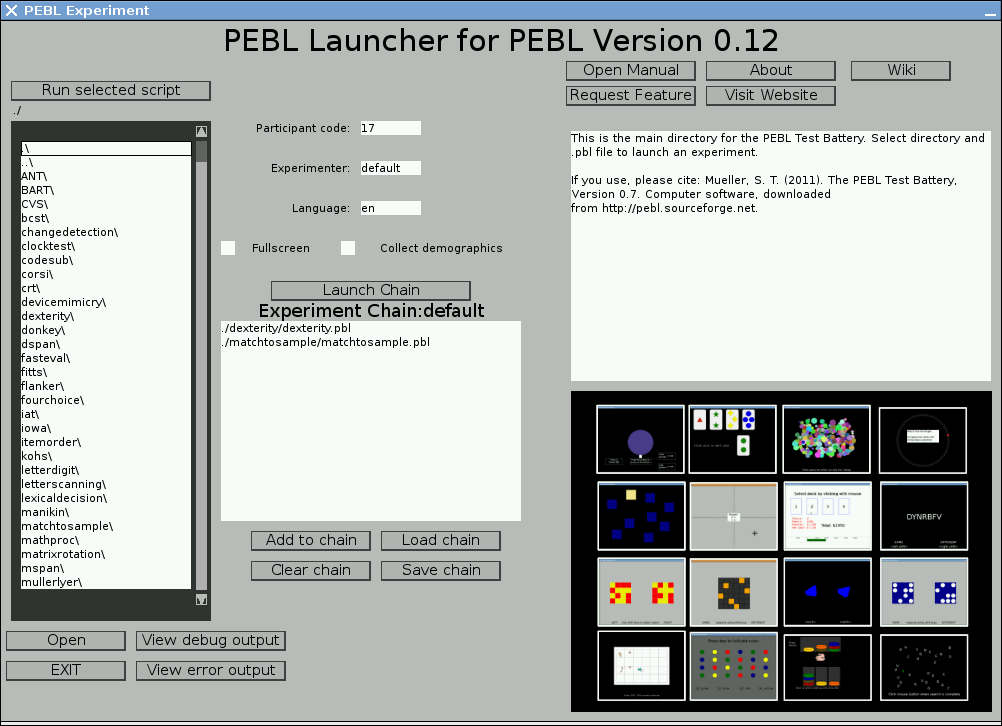
\includegraphics[scale=.35]{launcher.png} 
\end{figure}
\clearpage
\sect{History of the Launcher}
Prior to 2011, a front-end launcher was only available for PEBL on
Windows.  It was written in Visual Basic 6, which was old-fashioned,
single-platform, no longer supported by Microsoft, and created a
situation where a critical piece of PEBL infrastructure depended on a
non-free tool.  The main obstacle to a new launcher has always been:
PEBL needs a cross-platform launcher using a free software, and we
don't want to have to distribute a whole additional interpreter.  This
means that Python, wxBasic, TCL/TK, etc. were out of the
consideration.  Why couldn't there be an easy-to-use cross-platform
programming tool we could use?

As of PEBL Version 0.12, we found one: PEBL itself.  PEBL is not
really designed to create GUI applications, but it can be beat into
submission to do so.  For Version 0.12, enough filesystem access
functions and other features were available to make a reasonable
launcher.  Although the old-style launcher will probably still work,
it will no longer be supported.  The new launcher will not integrate
completely seamlessly into your operating system, but it is designed
to support the important functions of setting up and launching an
experiment.

\sect{How it works}
The simplest usage of the Launcher is that you use the file selector on
the left to choose a .pbl file, then click the button 'Run selected
script'' to run that experiment.  ONLY .pbl files and directories will
appear in the file window.
\clearpage
\sect{Features}

\begin{wrapfigure}{r}{0.5\textwidth}
 \vspace{-40pt}
  \begin{center}
    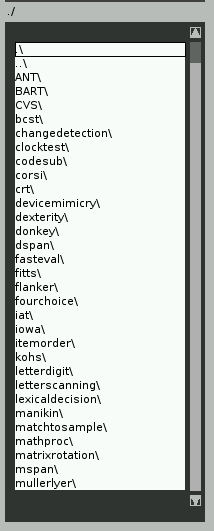
\includegraphics[scale=.5]{filebrowser.png} 
  \end{center}
  \caption{The PEBL Launcher File Browser.}
 \vspace{-50pt}
\end{wrapfigure}
\subsection{File browser}
On the left is a file browser.  It will only show .pbl files and
subdirectories.  To navigate to a subdirectory, simply click on the
directory to select it, then click on the selected directory.  To move
back up a directory, click on the '..\textbackslash' row.  When you have a .pbl file
selected, you can use the 'Run selected script' button to launch it.


\subsection{Participant code}
This will allow you to select the participant code you want sent to
any experiments you are about to run.  By default, PEBL saves the last
experiment code when you exit, and then reloads it the next time,
incrementing by one.  This makes it easier to avoid colliding
participant codes and overwriting data.  Participant code need not be
a number, but the launcher currently does not understand how to
increment non-numeric codes, and will probably restart at 1.  The plus button next to the 
code box will increment the current number by 1, which is useful if you are running multiple sessions in a row.

The automatic incrementation of participant code can be turned off by
opening the fileselect.pbl file and changing the variable gAutoSubcode
from 1 to 0.

When an experiment is launched, the specified code will be fed into
the experiment using the -s command-line option, and will be bound to
the gSubNum variable.  Some of the standard experiments will ask you
to enter a participant code regardless of whether you have one selected.
If that is the case, you should be able to edit the script to remove
the request to specify a participant code. However, most experiments in
the test battery should only ask the experimenter to specify a participant
code if the participant code is '0', which is what it will be when no -s
command is given.  So, if you are using code 0, many of the
experiments will ask you to enter a code after they launch.


\subsection{Experimenter code}
Many times, you may wish to keep track of the experimenter or research
assistant who collected the data.  Have them enter their name in the
'experimenter' window.  The name will be saved on exit.  The
experimenter code will be saved to the runlog file (see below). 

\subsection{Language}
Some experiments have instructions and stimuli that are translated
into different languages.  Enter your two-character language code in
the language box to tell the experiment what language to use. If your
chosen language is not available, the experiment will fall back to
English.  If you want to translate an experiment into your own
language, ask on the PEBL mailing list.

\subsection{Fullscreen Mode}
If you want to launch your experiment in full-screen mode to improve
video latency and to avoid distractions, check this box. The secret
escape key combo is ctrl-alt-shift-\textbackslash : hit these four to abort out of
an experiment before it is complete.

\subsection{Demographics Collection}
The U.S. NIMH requires a number of demographic variables for research
they fund. Checking this box will collect this data and save it to a
data log file called demographics-log.csv, prior to running your experiment or experiment chain.

\subsection{Experiment Chains}
The launcher allows you to set up a 'chain' of experiments that get run in sequence.  All the experiments will be run consecutively, with an identical subject code.  This is accomplished by running a separate instance of PEBL for each experiment.  The different experiments have no ability to communicate directly with one another.


\subsection{Saving Experiment Chains}
When you exit the launcher, the current experiment chain will get saved in the the current config file.  By default, this file is called default.config.  This same file is loaded when the launcher starts again, restoring your settings.  In addition, a chain can be saved with a different name, and loaded, either at start-up (by specifying the name of the config file with the -v command-line option), or by entering the name in the dialog that occurs when 'Load  Chain' is clicked.

\subsection{Loading Experiment Chains}
A previously saved experiment chain can be loaded using the 'load chain' button.  If a config file with that name exists, it will load the settings and the experiment chain in that file.  If no file exists with the specified name, it will change the name from 'default' (or whatever the current chain is called) to the specified name, and save the current configuration to the new configuration file on exit or when the 'save chain' button is clicked.

\subsection{Description and Screenshot}
On the right side of the launcher is a window that will show a screenshot and print a description of a script when it is highlighted.  These need to be created by hand for each script.

\subsection{Other buttons}
The launcher has a number of other buttons to help you use PEBL.
These include:
\begin{itemize}

\item \emph{Open} On the lower left, there is a button labeled ``Open''.  This
  will open a selected .pbl script in a text editor, and will open a
  directory in your system's file manager.  An easy way to look at or
  make changes to the script, or to locate data files after a script is run. 

\item \emph{View debug output} Whenever an experiment is run, any time
  you use the Print() function, it will print the resulting text to a
  file names stdout.txt the directory it was run in.  This button will
  open that file.

\item \emph{View error output} Whenever an experiment is run, the
  error and status messages are saved to a file called stderr.txt in
  the directory it was run in.  This button will open that file.

\item \emph{Exit} This will exit the launcher and save the current
  configuration options to the named experiment chain.

\item \emph{Open manual} This opens the PEBL .pdf manual.  The manual
  is located in different places on each platform, and will change
  names for each release.

\item \emph{About} This provides a short description of the launcher.

\item \emph{Visit Website}  This will take you to the main PEBL website.

\item \emph{Request Feature}  This takes you to the PEBL Fundry
  website, where you are able to request a feature (including new
  experiment scripts).  Fundry allows you to pledge a donation for
  your feature, allowing you to support PEBL and be a driver
  of its development.

\item \emph{Wiki} This button will take you to the PEBL wiki, and do
  its best to find a WIKI page related to the experiment you are
  looking at. They won't always exist, and if not, you can always sign
  in and make your own.

\end{itemize}

\sect{Launching an experiment}

To launch an experiment, navigate through the directories in the file listing box.  Only directories and files with the .pbl extension are shown in this box.  To open a directory, click once to move the highlight box onto the directory name, and a second time to open the directory.  When a new directory is opened, the first available .pbl file will be automatically selected.  To run that script, just press the 'Run Selected script' button above the file select box.  It will run with the specified parameter, including subject code, language, fullscreen mode.  In addition, if the 'collect demographics' button is selected, a demographic survey will happen prior to the study running.

\sect{Launching an experiment chain}
If you have a series of experiments you want to run, create an experiment chain and launch it using the 'Launch chain' button above the experiment chain selection box.  Tip: Use experiment chains even if you are are running just single experiment, with just a single experiment selected.  This give faster access and is less error-proned.

\sect{Translating the Launcher}
You can translate the launcher to your own language.  Open the launcher file (fileselect.pbl), and go to the end of the script, to a function named "GetStrings":
\begin{verbatim}
define GetStrings(lang)
{
   lang <- Uppercase(lang)
   if(lang == "EN")
   {
      gRunText <- "Run selected script"
      gOpenText <- "Open"
      gExitText <- "EXIT"
      gViewDebugText <- "View debug output"
      gViewErrorText <- "View error output"
      gAddToChainText <- "Add to Chain"
      gClearChainText <- "Clear Chain"
      gSaveChainText <- "Save Chain"
....
\end{verbatim}

The labels used in the launcher all appear here.  You should be able to just translate the text of each on into the language of your choice.  Send the translations back to the author so they can be incorporated into the next launcher version.  You can also make a section in the if statement for your particular language.  When you change the language in launcher, it will save that option and use your language of choice next time.

%%% Local Variables: 
%%% mode: latex
%%% TeX-master: "main"
%%% End: 

\include{testbattery}
\chapter{Detailed Function and Keyword Reference}
\label{sec:reference}

\setlength{\parindent}{0pt}

\newcommand{\rl}{\rule{\textwidth}{0.3mm}}

%% \newenvironment{desc}[1]
%%  {\begin{list}{}%
%%   {\renewcommand\makelabel[1]{{##1:}\hfil}%
%%    \settowidth\labelwidth{\makelabel{#1}}%
%%    \setlength\leftmargin{\labelwidth+\labelsep}}}%
%%  {\end{list}}

%\newenvironment{desc}[1]
%  {\begin{minipage}[b]{\linewidth}
%   \rl%
%   \vspace{3pt}%
%   \begin{list}{}%
%   {\renewcommand\makelabel[1]{{##1:}\hfil}%
%    \settowidth\labelwidth{\makelabel{#1}}%
%    \setlength\leftmargin{\labelwidth+\labelsep}}}%
%  {\end{list}%
%   \vspace{1pt}%
%   \end{minipage}%
%   }
\newenvironment{desc}[1]
  {
     \rl%
   \vspace{3pt}%
   \begin{list}{}%
   {\renewcommand\makelabel[1]{{##1:}\hfil}%
    \settowidth\labelwidth{\makelabel{#1}}%
    \setlength\leftmargin{\labelwidth+\labelsep}}}%
  {\end{list}%
   \vspace{1pt}%
   }


\vfill
\sect{Symbols}
\vfill


\begin{desc}{Name/Symbol}
\item[Name/Symbol] \verb!+!

\item[Description] Adds two expressions together.  Also,
concatenates strings together.

\item[Usage]
\begin{verbatim}
<num1> + <num2>
<string1> + <string2>
<string1> + <num1>
\end{verbatim}
 Using other types of variables will cause errors.

\item[Example]
\begin{verbatim}
33 + 322                   --> 355
"Hello" + " " + "World"    --> "Hello World"
"Hello" + 33 + 322.5       --> "Hello355.5"
33 + 322.5 + "Hello"       --> "33322.5Hello"
\end{verbatim}

\item[See Also]     \verb!-!, \texttt{ToString()}
\end{desc}


\begin{desc}{Name/Symbol}
\item[Name/Symbol] \verb+-+

\item[Description]  Subtracts one expression from another

\item[Usage]        \verb!<num1> - <num2>!

\item[Example]     

\item[See Also]

\end{desc}




\begin{desc}{Name/Symbol}

\item[Name/Symbol] \verb+/+ 

\item[Description]  Divides one expression by another

\item[Usage]        \verb+<expression> / <expression>+ 

\item[Example]
\begin{verbatim}
333 / 10    # == 33.3
\end{verbatim}

\item[See Also]

\end{desc} 



\begin{desc}{Name/Symbol}
   

\item[Name/Symbol] \verb+*+

\item[Description]        Multiplies two expressions together

\item[Usage]       \verb+<expression> * <expression>+

\item[Example]
\begin{verbatim}
32 * 2 # == 64
\end{verbatim}

\item[See Also]     

\end{desc}




\begin{desc}{Name/Symbol}

\item[Name/Symbol] \verb!^!

\item[Description]  Raises one expression to the power of  another expression

\item[Usage]       \verb!<expression> ^ <expression>!

\item[Example]
\begin{verbatim}
25 ^ 2  # == 625
\end{verbatim}

\item[See Also]    \texttt{Exp}, \texttt{NthRoot}

\end{desc}



\begin{desc}{Name/Symbol}

\item[Name/Symbol] \verb+;+ 

\item[Description]        Finishes a statement, can start new statement
                      on the same line (not needed at end of line)

\item[Usage]       

\item[Example]     

\item[See Also]

\end{desc}



\begin{desc}{Name/Symbol}     

\item[Name/Symbol] \verb!#!

\item[Description]   Comment indicator; anything until the next CR
	       following this character is ignored

\item[Usage]       

\item[Example]     

\item[See Also]

\end{desc} 



     
\begin{desc}{Name/Symbol}

\item[Name/Symbol] \verb!<-!                  

\item[Description]  The assignment operator.  Assigns a value to a variable\\
              N.B.: This two-character sequence takes the place of the
	      `\verb!=!' operator found in many programming languages.

\item[Usage]       

\item[Example]     

\item[See Also]  

\end{desc}   



\begin{desc}{Name/Symbol}

\item[Name/Symbol] \verb+( )+                  

\item[Description] Groups mathematical operations

\item[Usage]      \verb+(expression)+

\item[Example]
\begin{verbatim}
(3 + 22) * 4  # == 100
\end{verbatim}

\item[See Also]     

\end{desc}



\begin{desc}{Name/Symbol}

\item[Name/Symbol] \verb!{ }!                  

\item[Description] Groups a series of statements

\item[Usage]
\begin{verbatim}
{ statement1
  statement2
  statement3
}
\end{verbatim}
	     

\item[Example]     

\item[See Also]     
\end{desc}



\begin{desc}{Name/Symbol}

\item[Name/Symbol] \verb+[ ]+                 

\item[Description]  Creates a list. Closing \verb+]+ must be on
 	      same line as last element of list, even
	      for nested lists.

\item[Usage]       \verb+[<item1>, <item2>, ....]+
            

\item[Example]
\begin{verbatim}
[]                    #Creates an empty list
[1,2,3]               #Simple list
[[3,3,3],[2,2],0]     #creates a nested list structure
\end{verbatim}


\item[See Also]     \texttt{List()}
\end{desc}



\begin{desc}{Name/Symbol}

\item[Name/Symbol] 	\verb+<+ 

\item[Description] 	Less than.  Used to compare two numeric quantities.

\item[Usage]
\begin{verbatim}
3 < 5
3 < value
\end{verbatim}
             
\item[Example]
\begin{verbatim}
if(j < 33)
{
  Print ("j is less than 33.")
}
\end{verbatim}

See Also:     	\verb+>+, \verb+>=+, \verb+<=+, \verb+==+, \verb+~=+, \verb+!=+, \verb+<>+

\end{desc}





\begin{desc}{Name/Symbol}

\item[Name/Symbol] 	\verb!>!                    

\item[Description] 	Greater than. Used to compare two numeric quantities.

\item[Usage]
\begin{verbatim}
5 > 3
5 > value
\end{verbatim}

\item[Example]
\begin{verbatim}
if(j > 55)
{
 Print ("j is greater than 55.")
}
\end{verbatim}

\item[See Also]     	\verb+<+, \verb+>=+, \verb+<=+, \verb+==+, \verb+~=+, \verb+!=+, \verb+<>+
\end{desc}




\begin{desc}{Name/Symbol}

\item[Name/Symbol] 	\verb+<=+                   

\item[Description] 	Less than or equal to.

\item[Usage]
\begin{verbatim}
3<=5  
3<=value
\end{verbatim}

\item[Example]
\begin{verbatim}
if(j <= 33)
{
 Print ("j is less than or equal to 33.")
}
\end{verbatim}
	
\item[See Also]     	\verb+<, >, >=, ==, ~=, !=, <>+

\end{desc}



\begin{desc}{Name/Symbol}

\item[Name/Symbol] 	\verb+>=+                   

\item[Description] 	Greater than or equal to.

\item[Usage]
\begin{verbatim}
5>=3  
5>=value
\end{verbatim}

\item[Example]
\begin{verbatim}
if(j >= 55)
{
 Print ("j is greater than or equal to 55.")
}
\end{verbatim}

\item[See Also]     	\verb+<,+ \verb+>+, \verb+<=+, \verb+==+, \verb+~=+, \verb+!=+, \verb+<>+
\end{desc}



\begin{desc}{Name/Symbol}

\item[Name/Symbol] 	\verb+==+                   

\item[Description] 	Equal to.

\item[Usage]       	\verb+4 == 4+
		

\item[Example]
\begin{verbatim}
2 + 2 == 4
\end{verbatim}

\item[See Also]     	\verb+<,+ \verb+>+, \verb+>=+, \verb+<=+, \verb+~=+, \verb+!=+, \verb+<>+
\end{desc}



\begin{desc}{Name/Symbol}
\item[Name/Symbol]  	\verb+<>+, \verb+!=+, \verb+~=+

\item[Description]  	Not equal to.

\item[Usage]		

\item[Example]	

\item[See Also]     	\verb+<+, \verb+>+, \verb+>=+, \verb+<=+, \verb+==+

\end{desc}

\vfill
\newpage
\sect{A} 
\vfill

\begin{desc}{Name/Symbol}

\item[Name/Symbol] 	\verb+Abs()+

\item[Description]   	Returns the absolute value of the number.

\item[Usage]
\begin{verbatim}
Abs(<num>)
\end{verbatim}        

\item[Example]
\begin{verbatim}
Abs(-300)  	# ==300
Abs(23)    	# ==23
\end{verbatim}

\item[See Also]     	\verb+Round()+, \verb+Floor()+, \verb+AbsFloor()+, \verb+Sign()+, \verb+Ceiling()+
\end{desc}




\begin{desc}{Name/Symbol}

\item[Name/Symbol]  	\verb+AbsFloor()+

\item[Description]  	Rounds \verb+<num>+ toward 0 to an integer.

\item[Usage]       	
\begin{verbatim}
AbsFloor(<num>)
\end{verbatim}

\item[Example]
\begin{verbatim}
AbsFloor(-332.7)   	# == -332
AbsFloor(32.88)    	# == 32
\end{verbatim}

\item[See Also]     	\verb+Round()+, \verb+Floor()+, \verb+Abs()+, \verb+Sign()+, \verb+Ceiling()+
\end{desc}




\begin{desc}{Name/Symbol}

\item[Name/Symbol] 	\verb+ACos()+ 

\item[Description]  	Inverse cosine of \verb+<num>+, in degrees.

\item[Usage]
\begin{verbatim}
ACos(<num>)
\end{verbatim}

\item[Example]	

\item[See Also]    	\verb+Cos()+, \verb+Sin()+, \verb+Tan()+, \verb+ATan()+, \verb+ATan()+ 

\end{desc}


 


\begin{desc}{Name/Symbol}

\item[Name/Symbol]  	\verb+AddObject()+

\item[Description] 	Adds a widget to a parent window, at the top of the object stack.  Once added, the object will be drawn onto the parent last, meaning it will be on top of anything previously added. 

In general, objects can be added to other objects as well as windows.  For example, you can add drawing objects (circles, etc.) to an image to annotate the image and maintain its proper x,y coordinates.

Also, if you 're-add' an object that is already on a widget, it will get automatically removed from the window first.  This is an easy way to reorder elements on a screen.

\begin{verbatim}
AddObject(<obj>, <window>)
AddObject(<obj>, <canvas>)
AddObject(<obj>, <widget>)
\end{verbatim}

\item[Example]
\begin{verbatim}

define Start(p)
{
 win <- MakeWindow()
 img <- MakeImage("pebl.png")
 circ <- Circle(20,20,10,MakeColor("red"),1)
 AddObject(circ,img)
 AddObject(img,win)
 Move(img,100,100)
 Draw()
 WaitForAnyKeyPress()
}
\end{verbatim}



\item[See Also]    	\verb+RemoveObject()+
\end{desc}





\begin{desc}{Name/Symbol}
\item[Name/Symbol]  	\verb+and+
  
\item[Description]  	Logical and operator.

\item[Usage]       	
\begin{verbatim}
<expression> and <expression>
\end{verbatim}

\item[Example]	

\item[See Also]     	\verb+or+, \verb+not+

\end{desc}




\begin{desc}{Name/Symbol}

\item[Name/Symbol]  	\verb+Append+
  
\item[Description]  	Appends an item to a list.  Useful for constructing lists in conjunction with the loop statement.

Note: \texttt{Append()} is useful, but inefficent for large data structures, because it requires making a copy of the entire data list and then overwriting it, if you use
\texttt{list <- Append(list, item)}.  The overhead will be hardly noticeable unless you are building lists hundreds of elements long.  In that case you shuold either create the list upfront and use \texttt{SetElement}, or you \texttt{PushOnEnd} to modify the list directly.

\item[Usage] 
\begin{verbatim}
Append(<list>, <item>)
\end{verbatim}

\item[Example]
\begin{verbatim}
list <- Sequence(1,5,1)
double  <- []
loop(i, list)
{
 double <- Append(double, [i,i])
}
Print(double)
# Produces [[1,1],[2,2],[3,3],[4,4],[5,5]]
\end{verbatim}

\item[See Also]  \verb+SetElement()+ \verb+List()+, \verb+[ ]+, \verb+Merge()+, \verb+PushOnEnd+
\end{desc}



\begin{desc}{Name/Symbol}

\item[Name/Symbol]  	\verb+AppendFile+
  
\item[Description]  	Appends onto the end of \verb+<file1>+ the contents of \verb+<file2>+.  Useful for compiling pooled data at the end of an experiment.

\item[Usage] 
\begin{verbatim}
AppendFile(<file1>, <file2>)
\end{verbatim}

\item[Example]:

The following open ten consecutive files, writes 50 random numbers to each, then appends each to a master file:

\begin{verbatim}

 loop(j, Sequence(1,10,1))
   {
    file <- FileOpenWrite(j+".txt")
   loop(i,Sequence(1,50,1))
    {
       FilePrint(file,j+","+i+","+Random())
    }
    AppendFile("master.txt",j+".txt")
  }
\end{verbatim}

\item[See Also]     	\verb+FileOpenWrite()+
\end{desc}






\begin{desc}{Name/Symbol}

\item[Name/Symbol]  	\verb+ASin()+ 

\item[Description]  	Inverse Sine of \verb+<num>+, in degrees.

\item[Usage]
\begin{verbatim}
ASin(<num>)
\end{verbatim}

\item[Example]	

\item[See Also]    	 \verb+Cos()+, \verb+Sin()+, \verb+Tan()+, \verb+ATan()+, \verb+ACos()+, \verb+ATan()+ 
\end{desc}





\begin{desc}{Name/Symbol}

\item[Name/Symbol]  	\verb+ATan+ 

\item[Description]  	Inverse Tan of \verb+<num>+, in degrees.

\item[Usage]		

\item[Example]	

\item[See Also]    	\verb+Cos()+, \verb+Sin()+, \verb+Tan()+, \verb+ATan()+, \verb+ACos()+, \verb+ATan()+ 
\end{desc}

\vfill
\newpage
\sect{B} 
\vfill


\begin{desc}{Name/Symbol}
\item[Name/Symbol]  	\verb+Bezier+ 

\item[Description] Creates a smoothed line through the  points
specified by \verb+<xpoints>+, \verb+<ypoints>+. The lists \verb+<xpoints>+ and
\verb+<ypoints>+ are adjusted by  \verb+<x>+ and \verb+<y>+, so they
should be relative to 0, not the location you want the points to be at.

Like other drawn objects, the bezier must then be added to the window
to appear. <steps> denotes how smooth the approximation will be.

\item[Usage]		
\begin{verbatim}
  Bezier(<x>,<y>,<xpoints>,<ypoints>,
         <steps>,<color>)
\end{verbatim}

\item[Example]	
\begin{verbatim}
  win <- MakeWindow()
   #This makes a T
   xpoints <- [-10,10,10,20,20,-20,-20,-10]
   ypoints <- [-20,-20,40,40,50,50,40,40]
  p1 <-    Bezier(100,100,xpoints, ypoints,
           5, MakeColor("black"))
  AddObject(p1,win)
  Draw()
\end{verbatim}

\item[See Also]   
\verb+BlockE()+, \verb+Polygon()+, \verb+MakeStarPoints()+,
\verb+MakeNGonPoints()+
\end{desc}




\begin{desc}{Name/Symbol}

\item[Name/Symbol]  	\verb+BlockE+ 

\item[Description] Creates a polygon in the shape of a
 block E, pointing in one of four directions.
Arguments include position in window.
\begin{itemize}
\item \verb+<x>+ and \verb+<y>+ is the position of the center
\item \verb+<h>+ and \verb+<w>+ or the size of the E in pixels
\item \verb+<thickness>+ thickness of the E
\item \verb+<direction>+ specifies which way the E points:  1=right,
  2=down, 3=left, 4=up.
\item \verb+<color>+ is a color object (not just the name)
\end{itemize}

Like other drawn objects, the Block E must then be added to the window
to appear.

\item[Usage]		
\begin{verbatim}
 BlockE(x,y,h,w,thickness,direction,color)
\end{verbatim}

\item[Example]	
\begin{verbatim}
  win <- MakeWindow()
  e1 <- BlockE(100,100,40,80,10,1,MakeColor("black"))
  AddObject(e1,win)
  Draw()
\end{verbatim}

\item[See Also]   
\verb+Plus()+, \verb+Polygon()+, \verb+MakeStarPoints()+,
\verb+MakeNGonPoints()+
\end{desc}



\begin{desc}{Name/Symbol}
\item[Name/Symbol]  	\verb+break+

\item[Description]  	Breaks out of a loop immediately.

\item[Usage]        	break

\item[Example]
\begin{verbatim}
loop(i ,[1,3,5,9,2,7])
{
 Print(i)
 if(i == 3) 
        {
         break
        }
}
\end{verbatim}

\item[See Also]   	\verb+loop+, \verb+return+
\end{desc}

\vfill
\newpage
\sect{C}
\vfill

\begin{desc}{Name/Symbol}
\item[Name/Symbol]  	\verb+Ceiling()+

\item[Description] 	Rounds \verb+<num>+ up to the next integer.

\item[Usage]
\begin{verbatim}
Ceiling(<num>)
\end{verbatim}

\item[Example] 
\begin{verbatim}
Ceiling(33.23)  	# == 34
Ceiling(-33.02) 	# == -33
\end{verbatim}

\item[See Also]     	\verb+Round()+, \verb+Floor()+, \verb+AbsFloor()+, \verb+Ceiling()+
\end{desc}



\begin{desc}{Name/Symbol}
\item[Name/Symbol]  	\verb+ChooseN()+

\item[Description] Samples \verb+<number>+ items from list, returning
  a list in the original order. Items are sampled without replacement, so
  once an item is chosen it will not be chosen again. If
  \verb+<number>+ is larger than the length of the list, the entire
  list is returned in order.  It differs from \verb+SampleN+ in that
  \verb+ChooseN+ returns items in the order they appeared in the
  originial list, but \verb+SampleN+ is shuffled. 

\item[Usage]       	
\begin{verbatim}
ChooseN(<list>, <n>)
\end{verbatim}

\item[Example]   	
\begin{verbatim}

# Returns 5 numbers
ChooseN([1,1,1,2,2], 5)     

# Returns 3 numbers from 1 and 7:
ChooseN([1,2,3,4,5,6,7], 3) 

\end{verbatim}

\item[See Also]    	\verb+SampleN()+, \verb+SampleNWithReplacement()+, \verb+Subset()+
\end{desc}



\begin{desc}{Name/Symbol}
\item[Name/Symbol]	\verb+Circle()+

\item[Description] Creates a circle for graphing at x,y with radius r.
  Circles must be added to a parent widget before it can be drawn; it
  may be added to widgets other than a base window. The properties of
  circles may be changed by accessing their properties directly,
  including the FILLED property which makes the object an outline
  versus a filled shape.


\item[Usage]
\begin{verbatim}
Circle(<x>, <y>, <r>,<color>)
\end{verbatim}

\item[Example]	
\begin{verbatim}
  
  c <- Circle(30,30,20, MakeColor(green))
  AddObject(c, win)
  Draw()

\end{verbatim}
\item[See Also]	\verb+Square()+, \verb+Ellipse()+, \verb+Rectangle()+, \verb+Line()+
\end{desc}


\begin{desc}{Name/Symbol}
\item[Name/Symbol]	\verb+CheckForNetworkConnection()+

\item[Description] Checks to see if there is an incoming TCP/IP connection on a network that is opened using \verb+OpenNetworkListener+.  This is an alternative to the \verb+WaitForNetworkConnection+ function that allows more flexibility (and allows updating the during waiting for the connection).

\item[Usage]
\begin{verbatim}
net <- CheckForNetwokConnection(network)
\end{verbatim}

\item[Example]	
\begin{verbatim}
  network <-      OpenNetworkListener(4444) 
  time <- GetTime()
  while(not connected and (GetTime() < time + 5000))
   {
      connected <- CheckForNetwokConnection(network) 
   }

\end{verbatim}
\item[See Also]	\verb+OpenNetworkListener()+, \verb+Getdata()+, \verb+WaitForNetworkConnection()+, \verb+CloseNetwork()+
\end{desc}



\begin{desc}{Name/Symbol}
\item[Name/Symbol]  	\verb+ClearEventLoop()+ 

\item[Description]  Clears the event loop.  This function is currently experimental, and its usage may change in future versions of PEBL.

\item[Usage]       	
\begin{verbatim}
USAGE CURRENTLY UNDOCUMENTED
\end{verbatim}

\item[Example]	

\item[See Also] 
\verb+RegisterEvent()+, \verb+StartEventLoop()+
\end{desc}





\begin{desc}{Name/Symbol}
\item[Name/Symbol]	\verb+CloseNetworkConnection()+

\item[Description]	Closes network connection

\item[Usage]
\begin{verbatim}
   CloseNetwork(<network>)
\end{verbatim}

\item[Example]	

\begin{verbatim}
  net <- WaitForNetworkConnection("localhost",1234)
  SendData(net,"Watson, come here. I need you.")
  CloseNetworkConnection(net)
\end{verbatim}
Also see nim.pbl for example of two-way network connection.
\item[See Also]
  \verb+ConnectToIP+, \verb+ConnectToHost+,  \verb+WaitForNetworkConnection+, \\
  \verb+GetData+,  \verb+SendData+, \verb+ConvertIPString+
\end{desc}





\begin{desc}{Name/Symbol}
\item[Name/Symbol]	\verb+ConnectToHost()+

\item[Description]	Connects to a host computer waiting for a
  connection on <port>, returning a network object that can be used to
  communicate.  Host is a text hostname, like \verb+"myname.indiana.edu"+, or
  use \verb+"localhost"+ to specify your current computer.

\item[Usage]
\begin{verbatim}
   ConnectToHost(<hostname>,<port>)
\end{verbatim}

\item[Example]	

  See nim.pbl for example of two-way network connection.
\begin{verbatim}
  net <- ConnectToHost("localhost",1234)
  dat <- GetData(net,20)
  Print(dat)
  CloseNetworkConnection(net)
\end{verbatim}

\item[See Also]
  \verb+ConnectToIP+, \verb+GetData+, 
\verb+WaitForNetworkConnection+,\\
 \verb+SendData+, \verb+ConvertIPString+, \verb+CloseNetworkConnection+
\end{desc}



\begin{desc}{Name/Symbol}
\item[Name/Symbol]	\verb+ConnectToIP()+

\item[Description]	Connects to a host computer waiting for a
  connection on \verb+<port>+, returning a network object that can be used to
  communicate.  \verb+<ip>+ is a numeric ip address, which must be
  created with the \verb+ConvertIPString(ip)+ function. 

\item[Usage]
\begin{verbatim}
   ConnectToIP(<ip>,<port>)
\end{verbatim}

\item[Example]	

  See nim.pbl for example of two-way network connection.
\begin{verbatim}
  ip <- ConvertIPString("192.168.0.1")
  net <- ConnectToHost(ip,1234)
  dat <- GetData(net,20)
  Print(dat)
  CloseNetworkConnection(net)
\end{verbatim}

\item[See Also]
  \verb+ConnectToHost+, \verb+GetData+, \verb+WaitForNetworkConnection+,\\
   \verb+SendData+, \verb+ConvertIPString+, \verb+CloseNetworkConnection+
\end{desc}





\begin{desc}{Name/Symbol}
\item[Name/Symbol] \verb+ConvertIPString()+

\item[Description]	Converts an IP address specified as a string into
  an integer that can be used by ConnectToIP.

\item[Usage]
\begin{verbatim}
   ConvertIPString(<ip-as-string>)
\end{verbatim}

\item[Example]	

  See nim.pbl for example of two-way network connection.
\begin{verbatim}
  ip <- ConvertIPString("192.168.0.1")
  net <- ConnectToHost(ip,1234)
  dat <- GetData(net,20)
  Print(dat)
  CloseNetworkConnection(net)
\end{verbatim}

\item[See Also]
  \verb+ConnectToHost+, \verb+ConnectToIP+, \verb+GetData+, \\ \verb+WaitForNetworkConnection+,
   \verb+SendData+, \\\verb+CloseNetworkConnection+
\end{desc}





\begin{desc}{Name/Symbol}
\item[Name/Symbol] \verb+ConvexHull()+

\item[Description]	Computes the convex hull of a set of [x,y]
  points. It returns a set of points that forms the convex hull, with
  the first and last point identical.  A convex hull is the set of
  outermost points, such that a polygon connecting just those points
  will encompass all other points, and such that no angle is acute.
  It is used in MakeAttneave.

\item[Usage]
\begin{verbatim}
   ConvexHull(<list-of-x-y-points>)
\end{verbatim}

\item[Example]	
\begin{verbatim} 
pts <- [[0.579081, 0.0327737], 
         [0.0536094, 0.378258], 
         [0.239628, 0.187751], 
         [0.940625, 0.26526], 
         [0.508748, 0.840846],
         [0.352604, 0.200193], 
         [0.38684, 0.212413],
         [0.00114761, 0.768165],
         [0.432963, 0.629412]]
  Print(ConvexHull(pts))

\end{verbatim}

output:
\begin{verbatim}
[[0.940625, 0.26526]
, [0.508748, 0.840846]
, [0.00114761, 0.768165]
, [0.0536094, 0.378258]
, [0.239628, 0.187751]
, [0.579081, 0.0327737]
, [0.940625, 0.26526]

\end{verbatim}


\item[See Also]
  \verb+MakeAttneave+,

\end{desc}




\begin{desc}{Name/Symbol}
\item[Name/Symbol]  	\verb+Cos()+
			 
\item[Description] 	Cosine of \verb+<deg>+ degrees.

\item[Usage]		
\item[Example]	
\begin{verbatim}
  Cos(33.5)
  Cos(-32)
\end{verbatim}

\item[See Also]     	\verb+Sin()+, \verb+Tan()+, \verb+ATan()+, \verb+ACos()+, \verb+ATan()+
\end{desc}


\begin{desc}{Name/Symbol}
\item[Name/Symbol]  	\verb+Countdown()+
			 
\item[Description] 	Displays a 3-2-1 countdown on the screen in with 500 ms ISI.
\verb+CountDown+ temporarily hides whatever is on the screen. It is useful in orienting participants to
the first trial of a task.

\item[Usage]		
\begin{verbatim}
   CountDown(win)
\end{verbatim}

\item[Example]	
\begin{verbatim}
  win <- MakeWindow()
  MessageBox("Press any key to begin",win)
  CountDown(win)
  Trial()
\end{verbatim}

\item[See Also]   \verb+MessageBox+
\end{desc}



\begin{desc}{Name/Symbol}

\item[Name/Symbol] \verb+CR()+

\item[Description]  Produces \verb+<number>+ linefeeds which can be added to a
  string and printed or saved to a file.  CR is an abbreviation for ``Carriage Return''.

\item[Usage]\verb!CR(<number>)!

\item[Example]     
\begin{verbatim}
         Print("Number: "  Tab(1) + number  + CR(2))
         Print("We needed space before this line.")
\end{verbatim}
\item[See Also]
\verb+Format()+, \verb+Tab()+
\end{desc}






\begin{desc}{Name/Symbol}
\item[Name/Symbol]  	\verb+CrossFactorWithoutDuplicates()+

\item[Description] 	This function takes a single list, and returns a list of all 
			pairs, excluding the pairs that have two of the same item. 
			To achieve the same effect but include the duplicates, use: \\
			\verb+DesignFullCounterBalance(x,x)+.

\item[Usage]
\begin{verbatim}
CrossFactorWithoutDuplicates(<list>)
\end{verbatim}

\item[Example]
\begin{verbatim}
CrossFactorWithoutDuplicates([a,b,c]) 
# == [[a,b],[a,c],[b,a],[b,c],[c,a],[c,b]]
\end{verbatim}

\item[See Also] \verb+DesignFullCounterBalance()+, \verb+Repeat()+,\\ \verb+DesignBalancedSampling()+,
 \verb+DesignGrecoLatinSquare()+,\\
  \verb+DesignLatinSquare()+,  \verb+RepeatList()+, 
  \verb+LatinSquare()+,\\ \verb+Shuffle()+
\end{desc}


\begin{desc}{Name/Symbol}
\item[Name/Symbol]  	\verb+CumNormInv()+

\item[Description] 	This function takes a probability and returns the 
  corresponding z-score for the cumulative standard normal distribution.
  It uses an accurate numerical approximation from:\\
  \texttt{http://home.online.no/~pjacklam/notes/invnorm}
\item[Usage]
\begin{verbatim}
CumNormInv(<p>)
\end{verbatim}

\item[Example]
\begin{verbatim}

 Print(CumNormInv(0))    #= NA
  Print(CumNormInv(.01)) #= -2.32634
  Print(CumNormInv(.5))  #= 0
  Print(CumNormInv(.9))  #= 1.28
  Print(CumNormInv(1))   #= NA
\end{verbatim}

\item[See Also] \verb+NormalDensity()+, \verb+RandomNormal()+
\end{desc}


\vfill
\newpage
\sect{D}
\vfill

\begin{desc}{Name/Symbol}
\item[Name/Symbol]  	\verb+define+

\item[Description]  	Defines a user-specified function.

\item[Usage]
\begin{verbatim}
define functionname (parameters)
{
 statement1
 statement2
 statement3
       #Return statement is optional:
 return <value>
}
\end{verbatim}

\item[Example]    	See above.

\item[See Also]
\end{desc}   	



\begin{desc}{Name/Symbol}
\item[Name/Symbol]  	\verb+DegToRad()+

\item[Description]  	Converts degrees to radians.

\item[Usage]
\begin{verbatim}
DegToRad(<deg>)
\end{verbatim}

\item[Example]     	
\begin{verbatim}
DegToRad(180) # == 3.14159...
\end{verbatim}

\item[See Also]    	\verb+Cos()+, \verb+Sin()+, \verb+Tan()+, \verb+ATan()+, \verb+ACos()+, \verb+ATan()+ 
\end{desc}





\begin{desc}{Name/Symbol}
\item[Name/Symbol]  	\verb+DesignBalancedSampling()+

\item[Description] 	Samples elements ``roughly'' equally.
  		This function returns a list of repeated samples from
 		\verb+<treatment_list>+, such that each element in \verb+<treatment_list>+ 
		appears approximately equally.  Each element from 
		\verb+<treatment_list>+ is sampled once without replacement before 
		all elements are returned to the mix and sampling is repeated.  
		If there are no repeated items in \verb+<list>+, there will be no
 		consecutive repeats in the output.  The last repeat-sampling 
		will be truncated so that a \verb+<length>+-size list is returned.  
		If you don't want the repeated epochs this function provides, 
		Shuffle() the results.

\item[Usage]
\begin{verbatim}
DesignBalancedSampling(<list>, <length>)
\end{verbatim}

\item[Example]
\begin{verbatim}
DesignBalancedSampling([1,2,3,4,5],12)
## e.g., produces something like:
##    [5,3,1,4,2, 3,1,5,2,4, 3,1 ]
\end{verbatim}

\item[See Also]	\verb+CrossFactorWithoutDuplicates()+,
  \verb+Shuffle()+,\\ \verb+DesignFullCounterBalance()+,
  		\verb+DesignGrecoLatinSquare()+, \\
\verb+DesignLatinSquare()+, \verb+Repeat()+, 
		\verb+RepeatList()+,  \\\verb+LatinSquare()+

\end{desc}






\begin{desc}{Name/Symbol}

\item[Name/Symbol]	\verb+DesignFullCounterbalance()+

\item[Description]	This takes two lists as parameters, and returns a nested list 
		of lists that includes the full counterbalancing of both 
		parameter lists.  Use cautiously; this gets very large.

\item[Usage]
\begin{verbatim}
DesignFullCounterbalance(<lista>, <listb>)
\end{verbatim}

\item[Example]
\begin{verbatim}
a <- [1,2,3]
b <- [9,8,7]
DesignFullCounterbalance(a,b)	# == [[1,9],[1,8],[1,7],
				#     [2,9],[2,8],[2,7],
				#     [3,9],[3,8],[3,7]]
\end{verbatim}

\item[See Also] \verb+CrossFactorWithoutDuplicates()+,
  \verb+LatinSquare()+, \verb+Shuffle()+,
  \verb+DesignBalancedSampling()+, 
\\\verb+DesignGrecoLatinSquare()+, 
  \verb+DesignLatinSquare()+, \verb+Repeat()+, \verb+RepeatList()+,

\end{desc}






\begin{desc}{Name/Symbol}
\item[Name/Symbol]	\verb+DesignGrecoLatinSquare()+

\item[Description] This will return a list of lists formed by rotating
  through each element of the \verb+<treatment_list>+s, making a list
  containing all element of the list, according to a greco-latin
  square.  All lists must be of the same length.

\item[Usage]
\begin{verbatim}
DesignGrecoLatinSquare(<factor_list>, 
                       <treatment_list>, 
                       <treatment_list>)
\end{verbatim}

\item[Example]
\begin{verbatim}
x <- ["a","b","c"]
y <- ["p","q","r"]
z <- ["x","y","z"]
Print(DesignGrecoLatinSquare(x,y,z))
# produces:   	[[[a, p, x], [b, q, y], [c, r, z]], 
#               [[a, q, z], [b, r, x], [c, p, y]], 
#               [[a, r, y], [b, p, z], [c, q, x]]]
\end{verbatim}

\item[See Also] \verb+CrossFactorWithoutDuplicates()+, \verb+LatinSquare()+,\\
  \verb+DesignFullCounterBalance()+, \verb+DesignBalancedSampling()+,\\
  \verb+DesignLatinSquare()+, \verb+Repeat()+, \verb+RepeatList()+,
  \verb+Shuffle()+
\end{desc}




\begin{desc}{Name/Symbol}
\item[Name/Symbol]	\verb+DesignLatinSquare()+

\item[Description] This returns return a list of lists formed by
  rotating through each element of \verb+<treatment_list>+, making a
  list containing all element of the list. Has no side effect on input
  lists.  

\item[Usage]
\begin{verbatim}
DesignLatinSquare(<treatment1_list>, 
                  <treatment2_list>)
\end{verbatim}

\item[Example]
\begin{verbatim}
order <- [1,2,3]
treatment <- ["A","B","C"]
design <- DesignLatinSquare(order,treatment)
# produces: [[[1, A], [2, B], [3, C]],
#            [[1, B], [2, C], [3, A]],
#            [[1, C], [2, A], [3, B]]]
\end{verbatim}

\item[See Also] \verb+CrossFactorWithoutDuplicates()+,
  \verb+DesignFullCounterBalance()+, \verb+DesignBalancedSampling()+,
  \verb+DesignGrecoLatinSquare()+, \verb+Repeat()+, \verb+LatinSquare()+
  \verb+RepeatList()+, \verb+Shuffle()+, \verb+Rotate()+
\end{desc}




\begin{desc}{Name/Symbol}
\item[Name/Symbol]	\verb+Dist()+

\item[Description] Returns Euclidean distance between two points.
  Each point should be [x,y], and any additional items in the list are
  ignored.  


\item[Usage]
\begin{verbatim}
Dist(<xylist1>, <xylist2>)
\end{verbatim}

\item[Example]	
\begin{verbatim}
  p1 <- [0,0]
  p2 <- [3,4]
  d <- Dist(p1,p2)  #d is 5
\end{verbatim}
\item[See Also]	
\end{desc}





\begin{desc}{Name/Symbol}
\item[Name/Symbol]	\verb+Div()+

\item[Description]  	Returns round(\verb+<num>/<mod>+)

\item[Usage]
\begin{verbatim}
Div(<num>, <mod>)
\end{verbatim}

\item[Example]	

\item[See Also]	\verb+Mod()+
\end{desc}






\begin{desc}{Name/Symbol}
\item[Name/Symbol]	\verb+Draw()+

\item[Description]	Redraws the screen or a specific widget.

\item[Usage]
\begin{verbatim}
Draw()
Draw(<object>)
\end{verbatim}

\item[Example]	

\item[See Also]	\verb+DrawFor()+, \verb+Show()+, \verb+Hide()+
\end{desc}





\begin{desc}{Name/Symbol}
\item[Name/Symbol]	\verb+DrawFor()+

\item[Description] Draws a screen or widget, returning after
  \verb+<cycles>+ refreshes. This function currently does not work as
  intended in the SDL implementation, because of a lack of control
  over the refresh blank.  It may work in the future.

\item[Usage]
\begin{verbatim}
DrawFor( <object>, <cycles>)
\end{verbatim}

\item[Example]	

\item[See Also]	\verb+Draw()+, \verb+Show()+, \verb+Hide()+
\end{desc}


\vfill
\newpage
\sect{E}
\vfill

\begin{desc}{Name/Symbol}
\item[Name/Symbol]	\verb+EasyLabel()+

\item[Description] Creates and adds to the window location a label
  at specified location. Uses standard vera font with grey background.
   (May in the future get background color from window).
  Easy-to-use replacement for the \verb+MakeFont+,  ~\verb+MakeLabel+,
 ~ \verb+AddObject+, ~ \verb+Move+, steps you typically have to go through.

\item[Usage]
\begin{verbatim}
EasyLabel( <text>,<x>, <y>, <win>, <fontsize>)
\end{verbatim}

\item[Example]	
\begin{verbatim}
  win <- MakeWindow()
  lab <- EasyLabel("What?",200,100,win,12)
  Draw()
\end{verbatim}
\item[See Also]	
\verb+EasyTextBox()+, \verb+MakeLabel()+
\end{desc}




\begin{desc}{Name/Symbol}
\item[Name/Symbol]	\verb+EasyTextBox()+

\item[Description] Creates and adds to the window location a textbox
  at specified location. Uses standard vera font with white background.
  Easy-to-use replacement for the MakeFont,MakeTextBox,
  AddObject, Move, steps.

\item[Usage]
\begin{verbatim}
EasyTextBox( <text>,<x>, <y>, <win>,
             <fontsize>,<width>,<height>)
\end{verbatim}

\item[Example]	
\begin{verbatim}
  win <- MakeWindow()
  entry <- EasyTextBox("1 2 3 4 5",200,100,
                        win,12,200,50)
  Draw()
\end{verbatim}
\item[See Also]	
\verb+EasyLabel()+, \verb+MakeTextBox()+
\end{desc}



\begin{desc}{Name/Symbol}
\item[Name/Symbol]	\verb+Ellipse()+
  
\item[Description]	Creates a ellipse for graphing at x,y with radii
  rx and ry. Ellipses are only currently definable oriented in
  horizontal/vertical directions.  Ellipses  must be added
  to a parent widget before it can be drawn; it may be added to
  widgets other than a base window.  The properties of ellipses may be
  changed by accessing their properties directly, including the FILLED
  property which makes the object an outline versus a filled shape.

\item[Usage]
\begin{verbatim}
Ellipse(<x>, <y>, <rx>, <ry>,<color>)
\end{verbatim}

\item[Example]	
\begin{verbatim}
  
  e <- Ellipse(30,30,20,10, MakeColor(green))
  AddObject(e, win)
  Draw()

\end{verbatim}
\item[See Also]	\verb+Square()+, \verb+Circle()+, \verb+Rectangle()+, \verb+Line()+
\end{desc}


\begin{desc}{Name/Symbol}
\item[Name/Symbol]	\verb+EndOfFile()+

\item[Description]	Returns true if at the end of a file.

\item[Usage]
\begin{verbatim}
EndOfFile(<filestream>)
\end{verbatim}

\item[Example]
\begin{verbatim}
while(not EndOfFile(fstream))
{
 Print(FileReadLine(fstream))
}
\end{verbatim}

\item[See Also]	
\end{desc}


\begin{desc}{Name/Symbol}
\item[Name/Symbol]	\verb+EndOfLine()+

\item[Description]	Returns true if at end of line.

\item[Usage]
\begin{verbatim}
EndOfLine(<filestream>)
\end{verbatim}

\item[Example]	

\item[See Also]	
\end{desc}

\begin{desc}{Name/Symbol}
\item[Name/Symbol]	\verb+Enquote()+

\item[Description]	Surrounds the argument with quotes.  

\item[Usage]
\begin{verbatim}
Enquote("one two three")
\end{verbatim}

\item[Example]
\begin{verbatim}
 ##use to add quoted text to instructions.
 instructions <- "Respond whenever you see an "+ 
                  Enquote("X")

  ##Use it for saving data that may have spaces: 
  resp <-  GetInput(tb, "<enter>")
  FilePrint(fileout, Enquote(resp))

\end{verbatim}

\item[See Also]	
 gQuote 
\end{desc}





\begin{desc}{Name/Symbol}
\item[Name/Symbol]  	\verb+Exp()+

\item[Description]	$e$ to the power of \verb+<pow>+.

\item[Usage]
\begin{verbatim}
Exp(<pow>)
\end{verbatim}

\item[Example]
\begin{verbatim}
Exp(0) 		# == 1
Exp(3)		# == 20.0855
\end{verbatim}

\item[See Also]	\verb+Log()+
\end{desc}



\begin{desc}{Name/Symbol}
\item[Name/Symbol]	\verb+ExtractListItems()+

\item[Description]	Extracts items from a list, forming a new list. 
		The list \verb+<items>+ are the integers representing the
		indices that should be extracted.  
	     
\item[Usage]
\begin{verbatim}
ExtractListItems(<list>,<items>)
\end{verbatim}

\item[Example]
\begin{verbatim}
myList <- Sequence(101, 110, 1)
ExtractListItems(myList, [2,4,5,1,4])
# produces [102, 104, 105, 101, 104]
\end{verbatim}

\item[See Also]	\verb+Subset()+, \verb+SubList()+, \verb+SampleN()+
\end{desc}

\vfill
\newpage
\sect{F}
\vfill


\begin{desc}{Name/Symbol}
\item[Name/Symbol]	\verb+FileClose()+

\item[Description]	Closes a filestream  variable.  Be sure to 
		pass the variable name, not the filename.  

\item[Usage]
\begin{verbatim}
FileClose(<filestream>)
\end{verbatim}

\item[Example]
\begin{verbatim}
x <- FileOpenRead("file.txt")
# Do relevant stuff here.
FileClose(x)
\end{verbatim}

\item[See Also]	\verb+FileOpenAppend()+, \verb+FileOpenRead()+, \verb+FileOpenWrite()+

\end{desc}



\begin{desc}{Name/Symbol}
\item[Name/Symbol]	\verb+FileExists()+

\item[Description]	Checks whether a file exists.  Returns 1 if it exists, 0 otherwise.
\item[Usage]		
\begin{verbatim}
 FileExists(<path>)
\end{verbatim}

\item[Example]	
\begin{verbatim}
 filename <- "data-"+gSubNum+".csv"
 exists <-  FileExists(filename)
  if(exists)
   {
    MessageBox("Subject file already exists.  Please try a new one.",gWin) 
    SignalFatalError("filename already used")
   }
\end{verbatim}

\item[See Also]\verb+GetDirectoryListing()+, \verb+FileExists()+,       \verb+IsDirectory()+,        
   \verb+MakeDirectory()+      

\end{desc}




\begin{desc}{Name/Symbol}
\item[Name/Symbol]	\verb+FileOpenAppend()+

\item[Description] Opens a filename, returning a stream that can be
  used for writing information.  Appends if the file already exists.

\item[Usage]
\begin{verbatim}
FileOpenAppend(<filename>)
\end{verbatim}

\item[Example]	

\item[See Also]	\verb+FileClose()+, \verb+FileOpenRead()+, \verb+FileOpenWrite()+, 
\verb+FileOpenOverWrite()+
\end{desc}



\begin{desc}{Name/Symbol}
\item[Name/Symbol]	\verb+FileOpenOverwrite()+

\item[Description] Opens a filename, returning a stream that can be
  used for writing information.  Overwrites if file already exists.
  This function should not be used for opening data files; instead,
  use FileOpenWrite, which saves to a backup file if the specified
  file already exists.

\item[Usage]
\begin{verbatim}
FileOpenOverWrite(<filename>)
\end{verbatim}

\item[Example]	

\item[See Also]	\verb+FileClose()+, \verb+FileOpenAppend()+,
\verb+FileOpenRead()+  \verb+FileOpenWrite()+

\end{desc}


\begin{desc}{Name/Symbol}
\item[Name/Symbol]	\verb+FileOpenRead()+

\item[Description]  	Opens a filename, returning  a stream to be used 
		for reading information.

\item[Usage]
\begin{verbatim}
FileOpenRead(<filename>)
\end{verbatim}

\item[Example]	

\item[See Also]	\verb+FileClose()+, \verb+FileOpenAppend()+, \verb+FileOpenWrite()+, \verb+FileOpenOverWrite()+
\end{desc}


\begin{desc}{Name/Symbol}
\item[Name/Symbol]	\verb+FileOpenWrite()+

\item[Description] Opens a filename, returning a stream that can be
  used for writing information.  If the specified filename exists, it
  won't overwrite that file.  Instead, it will create a related
  filename, appending a -integer before the filename extension.


\item[Usage]
\begin{verbatim}
FileOpenWrite(<filename>)
\end{verbatim}

\item[Example]	

In the following example, test.txt gets created with the text
``testing 1'', and then a second file test-1.txt gets created with the
text ``testing 2''.

\begin{verbatim}
  f1 <- FileOpenWrite("test.txt")
  FilePrint(f1,"testing 1")
  FileClose(f1)
  f2 <- FileOpenWrite("test.txt")
  FilePrint(f2,"testing 2")
  FileClose(f2)
\end{verbatim}

\item[See Also]	\verb+FileClose()+, \verb+FileOpenAppend()+, \verb+FileOpenRead()+, \verb+FileOpenOverWrite()+
\end{desc}



\begin{desc}{Name/Symbol}
\item[Name/Symbol]	\verb+FilePrint()+

\item[Description]	Like \verb+Print+, but to a file.  Prints a string to a file, 
		with a carriage return at the end.  Returns a
  copy of the string it prints.
	
\item[Usage]
\begin{verbatim}
FilePrint(<filestream>, <value>)
\end{verbatim}

\item[Example]
\begin{verbatim}
FilePrint(fstream, "Another Line.")
\end{verbatim}

\item[See Also]	\verb+Print()+, \verb+FilePrint_()+
\end{desc}



\begin{desc}{Name/Symbol}
\item[Name/Symbol]	\verb+FilePrint_()+

\item[Description]	Like \verb+Print_+, but to a file.  Prints a
  string to a file,	without appending a newline character.  Returns a
  copy of the string it prints.
	
\item[Usage]
\begin{verbatim}
FilePrint_(<filestream>, <value>)
\end{verbatim}

\item[Example]
\begin{verbatim}
FilePrint_(fstream, "This line doesn't end.")
\end{verbatim}

\item[See Also]	\verb+Print_()+, \verb+FilePrint()+
\end{desc}


\begin{desc}{Name/Symbol}
\item[Name/Symbol]	\verb+FilePrintList()+

\item[Description]	Prints a list to a file, without the ','s or []
  characters. Puts a carriage return at the end.  Returns a string
  that was printed.  If a list contains other lists, the printing will
  wrap multiple lines and the internal lists will be printed as
  normal.  To avoid this, try FilePrintList(file,Flatten(list)).

\item[Usage]
\begin{verbatim}
FilePrintList(<filestream>, <list>)
\end{verbatim}

\item[Example]
\begin{verbatim}

FilePrintList(fstream, [1,2,3,4,5,5,5])
##
##  Produces:
##1 2 3 4 5 5 5
FilePrintList(fstream,[[1,2],[3,4],[5,6]])
#Produces:
# [1,2]
#,[3,4]
#,[5,6]

FilePrintList(fstream,Flatten([[1,2],[3,4],[5,6]]))
#Produces:
# 1 2 3 4 5 6


\end{verbatim}

\item[See Also]	\verb+Print()+, \verb+Print_()+, \verb+FilePrint()+, \verb+FilePrint_()+, \verb+PrintList()+,
\end{desc}



\begin{desc}{Name/Symbol}
\item[Name/Symbol]	\verb+FileReadCharacter()+

\item[Description]	Reads and returns a single character from a filestream.

\item[Usage]
\begin{verbatim}
FileReadCharacter(<filestream>)
\end{verbatim}

\item[Example]	

\item[See Also]	
   \verb+FileReadList()+, \verb+FileReadTable()+
   \verb+FileReadLine()+, 	\verb+FileReadText()+, 	\verb+FileReadWord()+,

\end{desc}



\begin{desc}{Name/Symbol}
\item[Name/Symbol]	\verb+FileReadLine()+

\item[Description]	Reads and returns a line from a file; all characters up
		until the next newline or the end of the file.

\item[Usage]
\begin{verbatim}
FileReadLine(<filestream>)
\end{verbatim}

\item[Example]	

\item[See Also]	

	\verb+FileReadCharacter()+,\verb+FileReadList()+, \verb+FileReadTable()+
	\verb+FileReadText()+, 	\verb+FileReadWord()+,

\end{desc}



\begin{desc}{Name/Symbol}
\item[Name/Symbol]  	\verb+FileReadList()+
 
\item[Description] Given a filename, will open it, read in all the
  items into a list (one item per line), and close the file afterward.
  Ignores blank lines or lines starting with \verb+#+.  Useful with a
  number of pre-defined data files stored in \verb+media/text/+.  See
  Section~\ref{sec:media}: Provided Media Files.

\item[Usage]
\begin{verbatim}
FileReadList(<filename>)
\end{verbatim}

\item[Example]
\begin{verbatim}
FileReadList("data.txt")
\end{verbatim}

\item[See Also]

	\verb+FileReadCharacter()+, \verb+FileReadTable()+
	\verb+FileReadLine()+, 	\verb+FileReadText()+, 	\verb+FileReadWord()+,

\end{desc}

\begin{desc}{Name/Symbol}
\item[Name/Symbol]	\verb+FileReadTable()+

\item[Description]	Reads a table directly from a file. Data in file should
		separated by spaces.  Reads each line onto a sublist,
		with space-separated tokens as items in sublist.  Ignores
		blank lines or lines beginning with \verb+#+. Optionally,
		specify a token separator other than space.

\item[Usage]
\begin{verbatim}
FileReadTable(<filename>, <optional-separator>)
\end{verbatim}

\item[Example]
\begin{verbatim}
a <- FileReadTable("data.txt")
\end{verbatim}

\item[See Also]	
	\verb+FileReadCharacter()+,\verb+FileReadList()+, 
	\verb+FileReadLine()+, 	\verb+FileReadText()+, 	\verb+FileReadWord()+,

\end{desc}



\begin{desc}{Name/Symbol}
\item[Name/Symbol]	\verb+FileReadText()+

\item[Description]	Returns all of the text from a file, ignoring any lines
		beginning with \verb+#+. Opens and closes the file transparently.

\item[Usage]
\begin{verbatim}
FileReadText(<filename>)
\end{verbatim}

\item[Example]
\begin{verbatim}
instructions <- FileReadText("instructions.txt")
\end{verbatim}

\item[See Also]	
	\verb+FileReadCharacter()+,\verb+FileReadList()+, \verb+FileReadTable()+
	\verb+FileReadLine()+, 	\verb+FileReadWord()+,

\end{desc}


\begin{desc}{Name/Symbol}
\item[Name/Symbol]	\verb+FileReadWord()+

\item[Description]	Reads and returns  a `word' from a file; the next
		connected stream of characters not including a \verb+' '+
		or a newline. Will not read newline characters.

\item[Usage]
\begin{verbatim}
FileReadWord(<filestream>)
\end{verbatim}

\item[Example]	

\item[See Also]	\verb+FileReadLine()+, \verb+FileReadTable()+, \verb+FileReadList()+
	\verb+FileReadCharacter()+,\verb+FileReadList()+, \verb+FileReadTable()+
	\verb+FileReadLine()+, 	\verb+FileReadText()+, 	\verb+FileReadWord()+,

\end{desc}

\begin{desc}{Name/Symbol}
\item[Name/Symbol]	\verb+Filter()+            

\item[Description] Returns a subset of \verb+<list>+, depending on whether the \verb+<filter>+ list is zero or nonzero.  Both arguments must be lists of the same length.

\item[Usage]		
\begin{verbatim}
Filter(<list>,<filter>)
\end{verbatim}

\item[Example]	
\begin{verbatim} 
  x <- [1,2,3,3,2,2,1]
  Print(Filter(x,[1,1,1,0,0,0,0])) ##==[1,2,3]
  Print(Filter(x,Match(x,1)))      ##== [1,1]
\end{verbatim}

\item[See Also]	\verb+Match()+, \verb+Subset()+, \verb+Lookup()+
\end{desc}


\begin{desc}{Name/Symbol}
\item[Name/Symbol]	\verb+FindInString()+

\item[Description]	Finds a token in a string, returning the position.

\item[Usage]
\begin{verbatim}
FindInString(<string>,<string>)
\end{verbatim}

\item[Example]
\begin{verbatim}
FindInString("about","bo") 	# == 2
\end{verbatim}

\item[See Also]	\verb+SplitString()+
\end{desc}



\begin{desc}{Name/Symbol}
\item[Name/Symbol]	\verb+First()+

\item[Description]	Returns the first item of a list.

\item[Usage]
\begin{verbatim}
First(<list>)
\end{verbatim}

\item[Example]
\begin{verbatim}
First([3,33,132])		# == 3
\end{verbatim}

\item[See Also]	\verb+Nth()+, \verb+Last()+
\end{desc}


\begin{desc}{Name/Symbol}
\item[Name/Symbol]	\verb+Flatten()+

\item[Description]
	Flattens nested list \verb+<list>+ to a single flat list.

\item[Usage]
\begin{verbatim}
Flatten(<list>)
\end{verbatim}

\item[Example]
\begin{verbatim}
Flatten([1,2,[3,4],[5,[6,7],8],[9]])	# == [1,2,3,4,5,6,7,8,9]
Flatten([1,2,[3,4],[5,[6,7],8],[9]])	# == [1,2,3,4,5,6,7,8,9]
\end{verbatim}

\item[See Also]	\verb+FlattenN()+, \verb+FoldList()+
\end{desc}



\begin{desc}{Name/Symbol}
\item[Name/Symbol]	\verb+FlattenN()+

\item[Description]	Flattens \verb+<n>+ levels of nested list \verb+<list>+. 

\item[Usage]
\begin{verbatim}
Flatten(<list>, <n>)
\end{verbatim}

\item[Example]
\begin{verbatim}
Flatten([1,2,[3,4],[5,[6,7],8],[9]],1) 
# == [1,2,3,4,5,[6,7],8,9]
\end{verbatim}

\item[See Also]	\verb+Flatten()+, \verb+FoldList()+
\end{desc}



\begin{desc}{Name/Symbol}
\item[Name/Symbol]	\verb+Floor()+

\item[Description]	Rounds \verb+<num>+ down to the next integer.

\item[Usage]
\begin{verbatim}
Floor(<num>)
\end{verbatim}

\item[Example]
\begin{verbatim}
Floor(33.23)	# == 33
Floor(3.999)  	# ==3
Floor(-32.23) 	# == -33
\end{verbatim}
 
\item[See Also]	\verb+AbsFloor()+, \verb+Round()+, \verb+Ceiling()+
\end{desc}

\begin{desc}{Name/Symbol}
\item[Name/Symbol]	\verb+FoldList()+

\item[Description]	Folds a list into equal-length sublists.

\item[Usage]
\begin{verbatim}
FoldList(<list>, <size>)
\end{verbatim}

\item[Example]
\begin{verbatim}
FoldList([1,2,3,4,5,6,7,8],2)	# == [[1,2],[3,4],[5,6],[7,8]]
\end{verbatim}
 
\item[See Also]	\verb+FlattenN()+, \verb+Flatten()+
\end{desc}


\begin{desc}{Name/Symbol}
\item[Name/Symbol]	\verb+Format()+            

\item[Description]	Formats the printing of values to ensure the
  proper spacing. It will either truncate or pad \verb+<value>+ with spaces
  so that it ends up exactly \verb+<length>+ characters long.  Character
  padding is at the end.
 
\item[Usage]
\begin{verbatim}
Format(<value>, <length>)
\end{verbatim}

\item[Example]	
\begin{verbatim}

  x <- 33.23425225
  y <- 23.3
  Print("["+Format(x,5)+"]")
  Print("["+Format(y,5)+"]")
  ## Output: 
  ## [33.23 ]
  ## [23.3  ]
\end{verbatim}
         

\item[See Also]	
\verb+CR()+ \verb+Tab()+
\end{desc}

\vfill
\newpage
\sect{G}
\vfill


\begin{desc}{Name/Symbol}
\item[Name/Symbol]	\verb+GetAngle()+

\item[Description]	Gets  an angle (in degrees) from (0,0) of an x,y coordinate


\item[Usage]
\begin{verbatim}
GetAngle(<x>,<y>)
\end{verbatim}

\item[Example]	
\begin{verbatim}
  ##point sprite in the direction of a click   
  sprite <- LoadImage("car.png")
  AddObject(sprite,gWin)
  Move(sprite,300,300)
  xy <- WaitForDownClick()
  newangle <- GetAngle(First(xy)-300,Second(xy)-300)
  sprite.rotation <- newangle
  Draw()
\end{verbatim}

\item[See Also]	\verb+DegtoRad+, \verb+RadToDeg+
\end{desc}


\begin{desc}{Name/Symbol}
\item[Name/Symbol]	\verb+GetAngle3()+

\item[Description]	Gets  an angle (in radians) of abc.


\item[Usage]
\begin{verbatim}
GetAngle3(<a>,<b>,<c>)
\end{verbatim}

\item[Example]	



\begin{verbatim}
   a <- [0.579081, 0.0327737]
   b <- [0.0536094, 0.378258]
   c <- [0.239628, 0.187751]

  Print(GetAngle3(a,b,c)) ## .2157

\end{verbatim}

\item[See Also]	\verb+DegtoRad+, \verb+RadToDeg+, \verb+GetAngle+, \verb+ToRight+
\end{desc}

\begin{desc}{Name/Symbol}
\item[Name/Symbol]	\verb+GetCurrentScreenResolution()+

\item[Description]	Returns an list of [width,height] specifying what the 
current computer screen resolution is.  This is used within the pebl launcher in order
to use the current resolution to run the experiment.

\item[Usage]
\begin{verbatim}
res <- GetCurrentScreenResolution()
\end{verbatim}

\item[Example]	

\begin{verbatim}
define Start(p)
{
   ## For testing, let's make the screen resolution a bit smaller than the 
   ## current one so that it doesn't get hidden by the bottom task bar
   ##
   res <- GetCurrentScreenResolution()
   gVideoWidth <- First(res)-100
   gVideoHeight <- Second(res)-100
   gWin <- MakeWindow()
   MessageBox("Window slightly smaller than screen",gWin)
}
\end{verbatim}


\item[See Also]	\verb+GetVideoModes()+
\end{desc}


\begin{desc}{Name/Symbol}
\item[Name/Symbol]	\verb+GetCursorPosition()+

\item[Description]	Returns an integer specifying where in a textbox the edit cursor is.  The value indicates which character it is on.

\item[Usage]
\begin{verbatim}
GetCursorPosition(<textbox>)
\end{verbatim}

\item[Example]	

\item[See Also]	\verb+SetCursorPosition()+, \verb+MakeTextBox()+, \verb+SetText()+
\end{desc}

\begin{desc}{Name/Symbol}
\item[Name/Symbol]	\verb+GetData()+

\item[Description]	Gets Data from network connection.  Example of
  usage in demo/nim.pbl.

\item[Usage]
\begin{verbatim}
val <- GetData(<network>,<size>)
\end{verbatim}

\item[Example]	

On 'server':
\begin{verbatim}
  net <- WaitForNetworkConnection("localhost",1234)
  SendData(net,"Watson, come here. I need you.")
  value <-  GetData(net,10)
  Print(value)

\end{verbatim}
On Client:
\begin{verbatim}
  net <- ConnectToHost("localhost",1234)
  value <-  GetData(net,20)
  Print(value)
##should print out "Watson, come here. I need you."
\end{verbatim}
\item[See Also]
  \verb+ConnectToIP+, \verb+ConnectToHost+, \verb+WaitForNetworkConnection+,
   \verb+SendData+, \verb+ConvertIPString+, \verb+CloseNetworkConnection+
\end{desc}




\begin{desc}{Name/Symbol}
\item[Name/Symbol]	\verb+GetDirectoryListing()+

\item[Description]	Returns a list of files and directories in a particular directory/folder.
\item[Usage]		
\begin{verbatim}
list <- GetDirectoryListing(<path>)
\end{verbatim}

\item[Example]	
\begin{verbatim}
 files <-  GetDirectoryListing("./")
\end{verbatim}

\item[See Also]\verb+GetDirectoryListing()+, \verb+FileExists()+,       \verb+IsDirectory()+,        
   \verb+MakeDirectory()+      

\end{desc}


  
\begin{desc}{Name/Symbol}
\item[Name/Symbol]	\verb+GetEasyChoice()+

\item[Description]	Hides what is on the screen and presents a textbox with
  specified message, and a series of options to select from. Returns element from corresponding position of the \verb+<output>+ list.  

\item[Usage]		
\begin{verbatim}
GetEasyChoice(<message>,<list-of-choices>,
             <output>,<window>)
\end{verbatim}

\item[Example]	
The code snippet below produces the following screen:\\
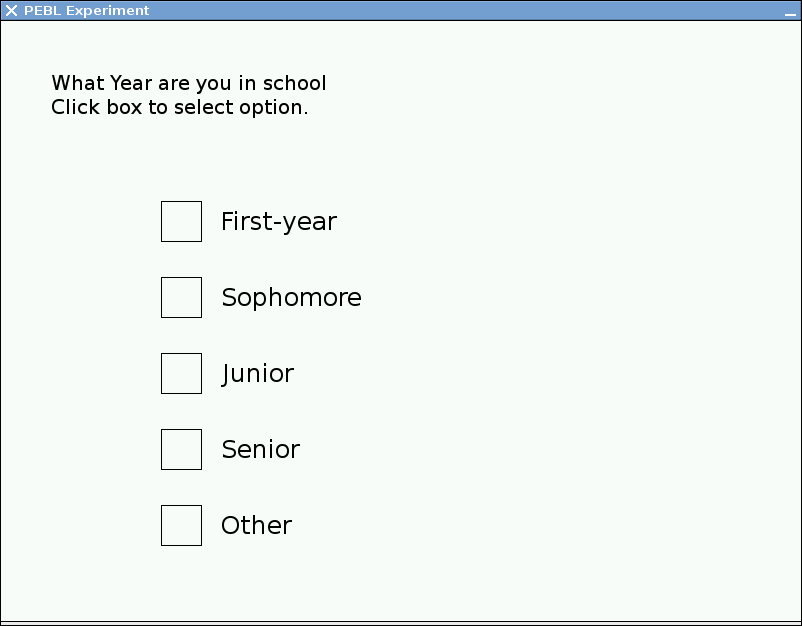
\includegraphics[scale=.25]{images/EasyChoice.png}
\begin{verbatim}
 gWin <- MakeWindow("white")
 inp <-  GetEasyChoice("What Year are you in school",
                        ["First-year","Sophomore",
                        "Junior","Senior","Other"],
                        [1,2,3,4,5],  gWin)
 

\end{verbatim}

\item[See Also]\verb+MessageBox+,\verb+GetEasyChoice+, \verb+EasyTextBox+
\end{desc}

  
  
  
\begin{desc}{Name/Symbol}
\item[Name/Symbol]	\verb+GetEasyInput()+

\item[Description]	Hides what is on the screen and presents a textbox with
  specified message, and a second text box to enter input.  Continues
  when 'enter' it hit at the end of text entry.

\item[Usage]		
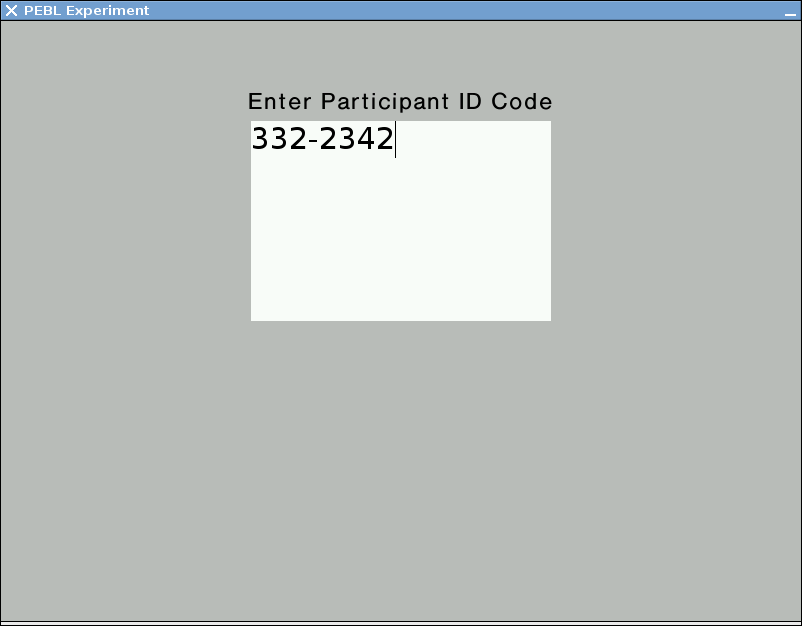
\includegraphics[scale=.25]{images/EasyInput.png}

\begin{verbatim}
GetEasyInput(<message>,<window>)
\end{verbatim}

\item[Example]	


\begin{verbatim}
 gWin <- MakeWindow()
 inp <-  GetEasyInput("Enter Participant ID Code",gWin)
\end{verbatim}

\item[See Also]\verb+MessageBox()+	\verb+GetEasyChoice()+, \verb+EasyTextBox()+
\end{desc}

\begin{desc}{Name/Symbol}
\item[Name/Symbol]	\verb+GetInput()+

\item[Description]	Allows user to type input into a textbox.

\item[Usage]
\begin{verbatim}
GetInput(<textbox>,<escape-key>)
\end{verbatim}

\item[Example]	

\item[See Also]	\verb+SetEditable()+, \verb+GetCursorPosition()+, \verb+MakeTextBox()+, \verb+SetText()+
\end{desc}


\begin{desc}{Name/Symbol}
\item[Name/Symbol] \verb+GetJoystickAxisState+ 

\item[Description]  
  This gets the state of a particular joystick axis.  You need to specify a joystick object, which is created with OpenJoystick().  You also need to specify the axis.  You can determine how many axes a joystick has with the GetNumJoystickAxes() function.  The function returns  a value between 1 and 32768.

\item[Usage]          \verb+GetJoystickAxisState(js,1)+ 

\item[Example]
See joysticktest.pbl in the demo\ directory

\item[See Also]
GetNumJoysticks(), OpenJoystick(), GetNumJoystickAxes()
GetNumJoystickBalls(), GetNumJoystickButtons(), GetNumJoystickHats()
GetJoystickAxisState(), GetJoystickHatState(), GetJoystickButtonState()
\end{desc} 

\begin{desc}{Name/Symbol}
\item[Name/Symbol] \verb+GetJoystickButtonState+ 

\item[Description]  
  This gets the state of a particular joystick button.  You need to specify a joystick object, which is created with OpenJoystick().  You also need to specify the button.  You can determine how many buttons a joystick has with the GetNumJoystickButtons() function.  The function returns either 0 (for unpressed) or 1 (for pressed).

\item[Usage]         \verb+GetJoystickButtonState(js,1)+ 

\item[Example]
See joysticktest.pbl in the demo\ directory
\item[See Also]
GetNumJoysticks(), OpenJoystick(), GetNumJoystickAxes()
GetNumJoystickBalls(), GetNumJoystickButtons(), GetNumJoystickHats()
GetJoystickAxisState(), GetJoystickHatState(), GetJoystickButtonState()
\end{desc} 

\begin{desc}{Name/Symbol}
\item[Name/Symbol] \verb+GetJoystickBallState+ 

\item[Description]  
	Not implemented.
\item[Usage]        \verb+GetJoystickBallState(js,1)+ 

\item[Example]
See joysticktest.pbl in the demo\ directory
\item[See Also]
GetNumJoysticks(), OpenJoystick(), GetNumJoystickAxes()
GetNumJoystickBalls(), GetNumJoystickButtons(), GetNumJoystickHats()
GetJoystickAxisState(), GetJoystickHatState(), GetJoystickButtonState()
\end{desc} 

\begin{desc}{Name/Symbol}
\item[Name/Symbol] \verb+GetJoystickHatState+ 

\item[Description]  

\item[Usage]        \verb+GetJoystickHatState(js,1)+ 
  This gets the state of a particular joystick hat.  You need to specify a joystick object, which is created with OpenJoystick().  You also need to specify the hat id.  You can determine how many hats a joystick has with the GetNumJoystickHats() function.  The function returns a value between 0 and 15, which is the sum of values specifying whether each primary NSEW direction is pressed.  The coding is: 0=no buttons; 1=N, 2=E, 4=S, 8=W.  Thus, if 1 is returned, the north hat button is pressed.  If 3 is returned, NorthEast.  If 12 is returned, SW, and so on.
  
\item[Example]
See joysticktest.pbl in the demo\ directory

\item[See Also]
GetNumJoysticks(), OpenJoystick(), GetNumJoystickAxes()
GetNumJoystickBalls(), GetNumJoystickButtons(), GetNumJoystickHats()
GetJoystickAxisState(), GetJoystickHatState(), GetJoystickButtonState()
\end{desc} 


\begin{desc}{Name/Symbol}
\item[Name/Symbol]	\verb+GetMouseCursorPosition()+

\item[Description] Gets the current x,y coordinates of the mouse
  pointer.

\item[Usage]
\begin{verbatim}
   GetMouseCursorPosition()
\end{verbatim}

\item[Example]	
\begin{verbatim}


 pos <- GetMouseCursorPosition()
\end{verbatim}


\item[See Also]
  \verb+ShowCursor+, \verb+WaitForMouseButton+,
  \verb+SetMouseCursorPosition+, \verb+GetMouseCursorPosition+
\end{desc}


\begin{desc}{Name/Symbol}
\item[Name/Symbol] \verb+GetMouseState()+

\item[Description] Gets the current x,y coordinates of the mouse
  pointer, plus the current state of the buttons.  Returns a 5-element list, with the first two indicating x,y position, the third is either 0 or 1 depending on if the left mouse is clicked, the fourth 0 or 2 depending on whether the middle mouse is clicked, and the fifth either 0 or 4 depending on whether the right mouse is clicked.

\item[Usage]
\verb+GetMouseState()+

\item[Example]	

\begin{verbatim}
define Start(p)
{
 
  win <- MakeWindow()
  i <- 1
  while(i < 100)
  {
    Draw()
    Print(GetMouseState())

    Wait(100)
    i <- i + 1

  }	
##Returns look like:
[417, 276, 0, 0, 0]
[495, 286, 0, 0, 0]
[460, 299, 0, 0, 0]
[428, 217, 0, 0, 0]
[446, 202, 0, 0, 4]
[446, 202, 1, 0, 0]
[446, 202, 1, 0, 0]
[446, 202, 0, 2, 0]

\end{verbatim}

\item[See Also]
  \verb+ShowCursor+ \verb+WaitForMouseButton+,
  \verb+SetMouseCursorPosition+, \verb+GetMouseCursorPosition+
\end{desc}


\begin{desc}{Name/Symbol}
\item[Name/Symbol]	\verb+GetNIMHDemographics()+

\item[Description]	Gets demographic information that are normally required for NIMH-related research.  Currently are gender (M/F/prefer not to say), ethnicity (Hispanic or not), and race (A.I./Alaskan, Asian/A.A., Hawaiian, black/A.A., white/Caucasian, other).  
		It then prints their responses in a single line in the demographics file, along with any special code you supply and a time/date stamp. This code might include a subject number, experiment number, or something else, but many informed consent forms assure the subject that this information cannot be tied back to them or their data, so be careful about what you record. The file output will look something like: 
\begin{verbatim}
---- 
31,Thu May 12 17:00:35 2011,F,hisp,asian,3331
32,Thu May 12 22:49:10 2011,M,nothisp,amind,3332
---- 
\end{verbatim}


	The first column is the user-specified code (in this 
	case, indicating the experiment number).  The middle columns 
	indicate date/time, and the last three columns indicate 
	gender (M, F, other), Hispanic (Y/N), and race.

\item[Usage]
\begin{verbatim}
GetNIMHDemographics(<code-to-print-out>,
                     <window>, <filename>)
\end{verbatim} 

\item[Example]
\begin{verbatim}
GetNIMHDemographics("x0413", gwindow, 
                    "x0413-demographics.txt")
\end{verbatim}

\item[See Also]	
\end{desc}


\begin{desc}{Name/Symbol}
\item[Name/Symbol] \verb+GetNumJoystickAxes+ 

\item[Description]  
  This gets the number of axes on a joystick.  You need to specify a joystick object, which is created with OpenJoystick(). 

\item[Usage]          \verb+GetNumJoystickAxes(js,1)+ 

\item[Example]
See joysticktest.pbl in the demo\ directory

\item[See Also]
GetNumJoysticks(), OpenJoystick(), GetNumJoystickAxes()
GetNumJoystickBalls(), GetNumJoystickButtons(), GetNumJoystickHats()
GetJoystickAxisState(), GetJoystickHatState(), GetJoystickButtonState()
\end{desc} 

\begin{desc}{Name/Symbol}
\item[Name/Symbol] \verb+GetNumJoystickBalls+ 

\item[Description]  
  This gets the number of joystick balls available on a particular joystick.  You need to specify a joystick object, which is created with OpenJoystick().  
  
\item[Usage]          \verb+GetNumJoystickBalls(js)+ 

\item[Example]
See joysticktest.pbl in the demo\ directory

\item[See Also]
GetNumJoysticks(), OpenJoystick(), GetNumJoystickAxes()
GetNumJoystickBalls(), GetNumJoystickButtons(), GetNumJoystickHats()
GetJoystickAxisState(), GetJoystickHatState(), GetJoystickButtonState()
\end{desc} 


\begin{desc}{Name/Symbol}
\item[Name/Symbol] \verb+GetNumJoystickButtons+ 

\item[Description]  
  This gets the number of joystick buttons available on a particular joystick.  You need to specify a joystick object, which is created with OpenJoystick(). 
\item[Usage]          \verb+GetNumJoystickButtons(js,1)+ 

\item[Example]
See joysticktest.pbl in the demo\ directory

\item[See Also]
GetNumJoysticks(), OpenJoystick(), GetNumJoystickAxes()
GetNumJoystickBalls(), GetNumJoystickButtons(), GetNumJoystickHats()
GetJoystickAxisState(), GetJoystickHatState(), GetJoystickButtonState()
\end{desc} 


\begin{desc}{Name/Symbol}
\item[Name/Symbol] \verb+GetNumJoystickHats+ 

\item[Description]  
  This gets the number of hats available on a particular joystick.  You need to specify a joystick object, which is created with OpenJoystick(). 
\item[Usage]          \verb+GetNumJoystickHats(js,1)+ 

\item[Example]
See joysticktest.pbl in the demo\ directory

\item[See Also]
GetNumJoysticks(), OpenJoystick(), GetNumJoystickAxes()
GetNumJoystickBalls(), GetNumJoystickButtons(), GetNumJoystickHats()
GetJoystickAxisState(), GetJoystickHatState(), GetJoystickButtonState()
\end{desc} 

\begin{desc}{Name/Symbol}
\item[Name/Symbol] \verb+GetNumJoysticks+ 

\item[Description]  
  This gets the number of joysticks available on a system. It returns an integer, which if greater than
  you can open a joystick using the OpenJoystick() function.. 
\item[Usage]          \verb+GetNumJoysticks()+ 

\item[Example]
See joysticktest.pbl in the demo\ directory

\item[See Also]
GetNumJoysticks(), OpenJoystick(), GetNumJoystickAxes()
GetNumJoystickBalls(), GetNumJoystickButtons(), GetNumJoystickHats()
GetJoystickAxisState(), GetJoystickHatState(), GetJoystickButtonState()
\end{desc} 



\begin{desc}{Name/Symbol}
\item[Name/Symbol]	\verb+GetPEBLVersion()+

\item[Description]	Returns a string describing which version of PEBL you are running.

\item[Usage]
\begin{verbatim}
GetPEBLVersion() 
\end{verbatim}

\item[Example]
\begin{verbatim}
Print(GetPEBLVersion())
\end{verbatim}

\item[See Also]	\verb+TimeStamp()+
\end{desc}


\begin{desc}{Name/Symbol}
\item[Name/Symbol]	\verb+GetPixelColor()+

\item[Description] Gets a color object specifying the color of a particular pixel on a widget.

\item[Usage]
\begin{verbatim}
color <- GetPixelColor(widget,x,y) 
\end{verbatim}

\item[Example]
\begin{verbatim}
  ##Judge brightness of a pixel
  img <- MakeImage("test.png")
  col <- GetPixelColor(img,20,20)
  hsv <- RGBtoHSV(col)
  Print(Third(hsv))

\end{verbatim}

\item[See Also]	\verb+SetPixel()+
\end{desc}


\begin{desc}{Name/Symbol}
\item[Name/Symbol] \verb+GetPPortState+ 

\item[Description]  
  Gets the parallel port state, as a list of 8 'bits' (1s or 0s).
  
\item[Usage]       
     \verb+out <- SetPPortState(pport)+ 
\item[Example]


\item[See Also]
\verb+COMPortGetByte+, \verb+COMPortSendByte+, \verb+OpenPPort+ \verb+OpenCOMPort+, \verb+SetPPortMode+, \verb+GetPPortState+ 
\end{desc} 



\begin{desc}{Name/Symbol}
\item[Name/Symbol]	\verb+GetSize()+

\item[Description] Returns a list of \verb+[height, width]+,
  specifying the size of the widget.
  The .width and .height properties can also be used instead of this function

\item[Usage]
\begin{verbatim}
GetSize(<widget>)
\end{verbatim}

\item[Example]
\begin{verbatim}
image <- MakeImage("stim1.bmp")
xy <- GetSize(image)
x <- Nth(xy, 1)
y <- Nth(xy, 2)
\end{verbatim}

\item[See Also]	
\end{desc}

\begin{desc}{Name/Symbol}
\item[Name/Symbol]	\verb+GetSubNum()+

\item[Description]	Creates dialog to ask user to input a subject code

\item[Usage]
\begin{verbatim}
GetSubNum(<win>)
\end{verbatim}

\item[Example]

\begin{verbatim}
## Put this at the beginning of an experiment, 
## after a window gWin has been defined.
##
 if(gSubNum == 0)
  {
    gSubNum <- GetSubNum(gWin)
  }
\end{verbatim}
Note: gSubNum can also be set from the command line.
\item[See Also]
\end{desc}

\begin{desc}{Name/Symbol}
\item[Name/Symbol]	\verb+GetSystemType()+

\item[Description]	Returns a string identify what type of computer system you are using. It will return either: OSX, LINUX, or WINDOWS.

\item[Usage]
\begin{verbatim}
GetSystemType()
\end{verbatim}

\item[Example]

\begin{verbatim}
## Put this at the beginning of an experiment, 
## after a window gWin has been defined.
   if(GetSystemType() == "WINDOWS")
    {
      SignalFatalError("Experiment untested on windows")
    }

\end{verbatim}

\item[See Also]
  \verb+SystemCall()+
\end{desc}



\begin{desc}{Name/Symbol}
\item[Name/Symbol]	\verb+GetText()+

\item[Description]	Returns the text stored in a text object 
		(either a textbox or a label).  The .text properties can also
  be used instead of this function.

\item[Usage]
\begin{verbatim}
GetText(<widget>)
\end{verbatim}

\item[Example]	

\item[See Also]	\verb+SetCursorPosition()+, \verb+GetCursorPosition()+, \verb+SetEditable()+, \verb+MakeTextBox()+
\end{desc}

\begin{desc}{Name/Symbol}
\item[Name/Symbol]	\verb+GetTextBoxCursorFromClick()+

\item[Description]	Returns the position (in characters) corresponding to a x,y click on a text box.  The X,Y position must be relative to the x,y position of the box, not absolute.  Once obtained, the cursor position can be set with SetCursorPosition().

\item[Usage]
\begin{verbatim}
GetTextBoxCursorFromClick(<widget>,<x>,<y>)
\end{verbatim}

\item[Example]	
\small
\begin{verbatim}
   win <- MakeWindow()
   tb <- EasyTextBox("Click here to set cursor position"
           ,100,100,win,200,200)
   Draw()
   WaitForClickOnTarget([tb],[1])
    #get the x and y cursor positions
   relx <- First(gClick) - (tb.x )
   rely <- Second(gClick) - (tb.y )
   tb.cursorpos <- GetTextBoxCursorFromClick(tb,
                                             relx,rely))
   Draw()
   WaitForAnyKeyPress()
\end{verbatim}
\normalsize
\item[See Also]	\verb+SetCursorPosition()+, \verb+GetCursorPosition()+, \verb+SetEditable()+, \verb+MakeTextBox()+
\end{desc}



\begin{desc}{Name/Symbol}
\item[Name/Symbol]	\verb+GetTime()+

\item[Description] Gets time, in milliseconds, from when PEBL was
  initialized.  Do not use as a seed for the RNG, because it will tend
  to be about the same on each run. Instead, use \verb+RandomizeTimer()+.

\item[Usage]
\begin{verbatim}
GetTime()
\end{verbatim}

\item[Example]
\begin{verbatim}
a <- GetTime()
WaitForKeyDown("A")
b <- GetTime()
Print("Response time is: " + (b - a))
\end{verbatim}

\item[See Also]	\verb+TimeStamp()+
\end{desc}


\begin{desc}{Name/Symbol}
\item[Name/Symbol]	\verb+GetVideoModes()+

\item[Description] Gets a list of useable video modes (in width/height pixel pairs), as supplied by the video driver.

\item[Usage]
\begin{verbatim}
  modes <- GetVideoModes()
\end{verbatim}

\item[Example]
\begin{verbatim}
Print(GetVideoModes)
##Might return:
[[1440, 900]
, [1360, 768]
, [1152, 864]
, [1024, 768]
, [960, 600]
, [960, 540]
, [840, 525]
, [832, 624]
, [800, 600]
, [800, 512]
, [720, 450]
, [720, 400]
, [700, 525]
]
\end{verbatim}

\item[See Also]	
\verb+GetCurrentScreenResolution+, \verb+gVideoWidth+,\verb+gVideoHeight+
\end{desc}


\begin{desc}{Name/Symbol}
\item[Name/Symbol]	\verb+GetVocalResponseTime+

\item[Description] This is a simple audio amplitude voice key controlled by two parameters  \emph{ONLY AVAILABLE ON WINDOWS AND LINUX}.

\item[Usage]
\begin{verbatim}
GetVocalResponseTime(buffer, 
                     timethreshold,
                     energythreshold)
\end{verbatim}
This is a simple function that fairly reliably gets an audio response time.  It works by recording audio to a buffer, and computing energy for 1-ms bins.  When enough bins (whose number/duration is set by timethreshald) in a row surpass an energy threshold (scaled from 0 to 1, set by energythreshold), recording will stop, and the voice key will return.  Reasonable values depend on the amount of noise in your microphone, and the types of vocal responses being made.  The return time will lag the detection time a bit, and so using the time it takes for the function to return is an unreliable measure of vocal response time.


It returns a list of three elements:

\begin{itemize}
\item Response time (in ms),
\item End time (using ms counter),
\item Responded flag: either 0 or 1, depending on whether the key was tripped,
\end{itemize}

If the responded flag is 0, the other two numbers will be as well.

See number-stroop.pbl in the stroop directory of the test battery and testaudioin.pbl in demo/ for examples.


\item[Example]	
\begin{verbatim}

  buffer <- MakeAudioInputBuffer(5000)
  resp0 <-  GetVocalResponseTime(buffer,.35, 200)
  SaveAudioToWaveFile("output.wav",buffer)
  
\end{verbatim}
\item[See Also] 	\verb+MakeAudioInputBuffer()+, \verb+SaveAudioToWaveFile()+,
\end{desc}




\vfill
\newpage
\sect{H}
\vfill


\begin{desc}{Name/Symbol}
\item[Name/Symbol]	\verb+Hide()+ 

\item[Description]	Makes an object invisible, so it will not be drawn.

\item[Usage]
\begin{verbatim}
Hide(<object>)
\end{verbatim}

\item[Example]
\begin{verbatim}
window <- MakeWindow()
image1  <- MakeImage("pebl.bmp")
image2  <- MakeImage("pebl.bmp")
AddObject(image1, window)
AddObject(image2, window)
Hide(image1)
Hide(image2)
Draw()		# empty screen will be drawn.
	
Wait(3000)
Show(image2)
Draw()		# image2 will appear.

Hide(image2)
Draw()		# image2 will disappear.

Wait(1000)
Show(image1)
Draw()		# image1 will appear.
\end{verbatim}
 
\item[See Also]	\verb+Show()+
\end{desc}

\vfill
\newpage
\sect{I}
\vfill


\begin{desc}{Name/Symbol}
\item[Name/Symbol]	\verb+if+ 

\item[Description]	Simple conditional test.

\item[Usage]
\begin{verbatim}
if(test)
{
 statements
 to
 be 
 executed
}
\end{verbatim}

\item[Example]	

\item[See Also]	
\end{desc}

\vfill

\begin{desc}{Name/Symbol}
\item[Name/Symbol]	\verb+if...elseif...else+            

\item[Description] Complex conditional test.  Be careful of spacing
  the else---if you put carriage returns on either side of it, you
  will get a syntax error. The \verb+elseif+ is optional, but
  multiple \verb+elseif+ statements can be strung together.  The
  \verb+else+ is also optional, although only one can appear.

\item[Usage]
\begin{verbatim}
if(test)
{
 statements if true
} elseif (newtest) {
 statements if newtest true; test false
} else {
 other statements
} 
\end{verbatim}

\item[Example]	
\begin{verbatim}
 if(3 == 1) {
             Print("ONE")
  }elseif(3==4){
             Print("TWO")
  }elseif(4==4){
             Print("THREE")
  }elseif(4==4){
             Print("FOUR")
  }else{Print("FIVE")}
\end{verbatim}
\item[See Also]	
if
\end{desc}


\begin{desc}{Name/Symbol}
\item[Name/Symbol]	\verb+Insert()+

\item[Description] Inserts an element into a list at a specified
  position, returning the new list. The original list in unchanged.

\item[Usage]	
\begin{verbatim}
Insert(<[list]>,<item>,<position>)	
\end{verbatim}
\item[Example]	

\begin{verbatim}
  x <- [1,2,3,5]
  y <- Insert(x,1,4)  
  ##y== [1,2,3,1,5]  
\end{verbatim}

\item[See Also]	
\verb+List()+, \verb+Merge+, \verb+Append+

\end{desc}



\begin{desc}{Name/Symbol}
\item[Name/Symbol]	\verb+Inside()+

\item[Description] Determines whether an \verb+[x,y]+ point is inside another
  object.  Will operate correctly for rectangles, squares, circles,
  textboxes, images, and labels. \verb+[xylist]+ can be a list containing
  [x,y], and if it is longer the other points will be ignored (such as
  the list returned by \verb+WaitForMouseButton()+.  Returns 1 if inside, 0
  if not inside.

\item[Usage]
\begin{verbatim}
Inside(<[xylist]>,<object>)	
\end{verbatim}

\item[Example]	

\begin{verbatim}
      button <- EasyLabel("Click me to continue", 100,100,gWin,12)

      continue <- 1
      while(continue)
      {
         xy <- WaitForMouseButton()
         continue <- Inside(xy,button)
      }
\end{verbatim}

\item[See Also]	
\verb+WaitForMouseButton()+, \verb+GetMouseCursorPosition+

\end{desc}

\begin{desc}{Name/Symbol}
\item[Name/Symbol]	\verb+IsAnyKeyDown()+

\item[Description]	

\item[Usage]		
\begin{verbatim}
  IsAnyKeyDown()
\end{verbatim}

\item[Example]	

\item[See Also]	
\end{desc}

\begin{desc}{Name/Symbol}
\item[Name/Symbol]	\verb+IsAudioOut()+

\item[Description]	Tests whether \verb+<variant>+ is a AudioOut stream.

\item[Usage]
\begin{verbatim}
IsAudioOut(<variant>)
\end{verbatim}

\item[Example]
\begin{verbatim}
if(IsAudioOut(x))
{
 Play(x)
}
\end{verbatim}

\item[See Also] \verb+IsColor()+, \verb+IsImage()+,
  \verb+IsInteger()+, \verb+IsFileStream()+, \verb+IsFloat()+,
  \verb+IsFont()+, \verb+IsLabel()+, \verb+IsList()+,
  \verb+IsNumber()+, \verb+IsString()+, \verb+IsTextBox()+,
  \verb+IsWidget()+
\end{desc}


\begin{desc}{Name/Symbol}
\item[Name/Symbol]	\verb+IsCanvas()+

\item[Description]	Tests whether \verb+<variant>+ is a Canvas widget.

\item[Usage]
\begin{verbatim}
IsCanvas(<variant>)
\end{verbatim}

\item[Example]
\begin{verbatim}
if(IsCanvas(x)
{
   SetPixel(x,10,10,MakeColor("red"))
}
\end{verbatim}

\item[See Also] \verb+IsAudioOut()+, \verb+IsImage()+,
  \verb+IsInteger()+, \verb+IsFileStream()+, \verb+IsFloat()+,
  \verb+IsFont()+, \verb+IsLabel()+, \verb+IsList()+,
  \verb+IsNumber()+, \verb+IsString()+, \verb+IsTextBox()+, \verb+IsText()+
  \verb+IsWidget()+, \verb+IsWindow()+
\end{desc}



\begin{desc}{Name/Symbol}
\item[Name/Symbol]	\verb+IsColor()+

\item[Description]	Tests whether \verb+<variant>+ is a Color.

\item[Usage]
\begin{verbatim}
IsColor(<variant>)
\end{verbatim}

\item[Example]
\begin{verbatim}
if(IsColor(x)
{
 gWin <- MakeWindow(x)
}
\end{verbatim}

\item[See Also] \verb+IsAudioOut()+, \verb+IsImage()+,
  \verb+IsInteger()+, \verb+IsFileStream()+, \verb+IsFloat()+,
  \verb+IsFont()+, \verb+IsLabel()+, \verb+IsList()+,
  \verb+IsNumber()+, \verb+IsString()+, \verb+IsTextBox()+,
  \verb+IsWidget()+, \verb+IsWindow()+
\end{desc}


\begin{desc}{Name/Symbol}
\item[Name/Symbol]	\verb+IsDirectory()+

\item[Description]	Determines whether a named path is a directory.  Returns 1 if it exists and is a directory, and 0 otherwise.
\item[Usage]		
\begin{verbatim}
 IsDirectory(<path>)
\end{verbatim}

\item[Example]	
\begin{verbatim}
 filename <- "data-"+gSubNum+".csv"
 exists <-  FileExists(filename)
  if(exists)
   {
    out <-    IsDirectory(filename)
    Print(out)
   }
\end{verbatim}

\item[See Also]\verb+GetDirectoryListing()+, \verb+FileExists()+,       \verb+IsDirectory()+,        
   \verb+MakeDirectory()+      

\end{desc}


\begin{desc}{Name/Symbol}
\item[Name/Symbol]	\verb+IsImage()+

\item[Description]	Tests whether \verb+<variant>+ is an Image.

\item[Usage]
\begin{verbatim}
IsImage(<variant>)
\end{verbatim}

\item[Example]	
\begin{verbatim}
if(IsImage(x))
{
 AddObject(gWin, x)
}
\end{verbatim}

\item[See Also] \verb+IsAudioOut()+, \verb+IsColor()+,
  \verb+IsInteger()+, \verb+IsFileStream()+, \verb+IsFloat()+,
  \verb+IsFont()+, \verb+IsLabel()+, \verb+IsList()+,
  \verb+IsNumber()+, \verb+IsString()+, \verb+IsTextBox()+,
  \verb+IsWidget()+
\end{desc}



\begin{desc}{Name/Symbol}
\item[Name/Symbol]	\verb+IsInteger()+

\item[Description] Tests whether \verb+<variant>+ is an integer type.
  Note: a number represented internally as a floating-point type whose
  is an integer will return false.  Floating-point numbers can be
  converted to internally- represented integers with the
  \verb+ToInteger()+ or \verb+Round()+ commands.
 
\item[Usage]		
\begin{verbatim}
IsInteger(<variant>)
\end{verbatim}

\item[Example]
\begin{verbatim}
x <- 44
y <- 23.5
z <- 6.5
test <- x + y + z 
	
IsInteger(x)		# true
IsInteger(y)		# false
IsInteger(z)		# false
IsInteger(test)		# false
\end{verbatim}

\item[See Also] \verb+IsAudioOut()+, \verb+IsColor()+,
  \verb+IsImage()+, \verb+IsFileStream()+, \verb+IsFloat()+,
  \verb+IsFont()+, \verb+IsLabel()+, \verb+IsList()+,
  \verb+IsNumber()+, \verb+IsString()+, \verb+IsTextBox()+,
  \verb+IsWidget()+
\end{desc}



\begin{desc}{Name/Symbol}
\item[Name/Symbol]	\verb+IsFileStream()+

\item[Description]	Tests whether \verb+<variant>+ is a FileStream object.

\item[Usage]		
\begin{verbatim}
IsFileStream(<variant>)
\end{verbatim}

\item[Example]
\begin{verbatim}
if(IsFileStream(x))
{
 Print(FileReadWord(x)
}
\end{verbatim}

\item[See Also] \verb+IsAudioOut()+, \verb+IsColor()+,
  \verb+IsImage()+, \verb+IsInteger()+, \verb+IsFloat()+,
  \verb+IsFont()+, \verb+IsLabel()+, \verb+IsList()+,
  \verb+IsNumber()+, \verb+IsString()+, \verb+IsTextBox()+,
  \verb+IsWidget()+
\end{desc}



\begin{desc}{Name/Symbol}
\item[Name/Symbol]	\verb+IsFloat()+

\item[Description] Tests whether \verb+<variant>+ is a floating-point
  value. Note that floating-point can represent integers with great
  precision, so that a number appearing as an integer can still be a
  float.

\item[Usage]
\begin{verbatim}
IsFloat(<variant>)
\end{verbatim}

\item[Example]
\begin{verbatim}
x <- 44
y <- 23.5
z <- 6.5
test <- x + y + z 

IsFloat(x)     	# false
IsFloat(y)     	# true
IsFloat(z)     	# true
IsFloat(test)  	# true
\end{verbatim}

\item[See Also] \verb+IsAudioOut()+, \verb+IsColor()+,
  \verb+IsImage()+, \verb+IsInteger()+, \verb+IsFileStream()+,
  \verb+IsFont()+, \verb+IsLabel()+, \verb+IsList()+,
  \verb+IsNumber()+, \verb+IsString()+, \verb+IsTextBox()+,
  \verb+IsWidget()+
\end{desc}



\begin{desc}{Name/Symbol}
\item[Name/Symbol]	\verb+IsFont()+

\item[Description]	Tests whether \verb+<variant>+ is a Font object.

\item[Usage]
\begin{verbatim}
IsFont(<variant>)
\end{verbatim}

\item[Example]	
\begin{verbatim}
if(IsFont(x))
{
 y <- MakeLabel("stimulus", x)
}
\end{verbatim}

\item[See Also] \verb+IsAudioOut()+, \verb+IsColor()+,
  \verb+IsImage()+, \verb+IsInteger()+, \verb+IsFileStream()+,
  \verb+IsFloat()+, \verb+IsLabel()+, \verb+IsList()+,
  \verb+IsNumber()+, \verb+IsString()+, \verb+IsTextBox()+,
  \verb+IsWidget()+
\end{desc}



\begin{desc}{Name/Symbol}
\item[Name/Symbol]	\verb+IsKeyDown()+

\item[Description]	

\item[Usage]		

\item[Example]	

\item[See Also]	\verb+IsKeyUp()+
\end{desc}

\begin{desc}{Name/Symbol}
\item[Name/Symbol]	\verb+IsKeyUp()+

\item[Description]	

\item[Usage]		

\item[Example]	

\item[See Also]	\verb+IsKeyDown()+
\end{desc}

\begin{desc}{Name/Symbol}
\item[Name/Symbol]	\verb+IsLabel()+

\item[Description]	Tests whether \verb+<variant>+ is a text Label object.

\item[Usage]		
\begin{verbatim}
IsLabel(<variant>)
\end{verbatim}

\item[Example]	
\begin{verbatim}
if(IsLabel(x)
{
 text <- GetText(x)
}
\end{verbatim}

\item[See Also] \verb+IsAudioOut()+, \verb+IsColor()+,
  \verb+IsImage()+, \verb+IsInteger()+, \verb+IsFileStream()+,
  \verb+IsFloat()+, \verb+IsFont()+, \verb+IsList()+,
  \verb+IsNumber()+, \verb+IsString()+, \verb+IsTextBox()+,
  \verb+IsWidget()+
\end{desc}

\begin{desc}{Name/Symbol}
\item[Name/Symbol]	\verb+IsList()+

\item[Description]	Tests whether \verb+<variant>+ is a PEBL list.

\item[Usage]
\begin{verbatim}
IsList(<variant>)
\end{verbatim}

\item[Example]	
\begin{verbatim}
if(IsList(x))
{
 loop(item, x)
 {
  Print(item)
 }
}
\end{verbatim}

\item[See Also] \verb+IsAudioOut()+, \verb+IsColor()+,
  I\verb+sImage()+, \verb+IsInteger()+, \verb+IsFileStream()+,
  \verb+IsFloat()+, \verb+IsFont()+, \verb+IsLabel()+,
  \verb+IsNumber()+, \verb+IsString()+, \verb+IsTextBox()+,
  \verb+IsWidget()+
\end{desc}

\begin{desc}{Name/Symbol}
\item[Name/Symbol]	\verb+IsMember()+

\item[Description]	Returns true if \verb+<element>+ is a member of \verb+<list>+.

\item[Usage]		
\begin{verbatim}
IsMember(<element>,<list>)
\end{verbatim}

\item[Example]	
\begin{verbatim}
IsMember(2,[1,4,6,7,7,7,7])		# false
IsMember(2,[1,4,6,7,2,7,7,7]) 		# true
\end{verbatim}

\item[See Also]	
\end{desc}

\begin{desc}{Name/Symbol}
\item[Name/Symbol]	\verb+IsNumber()+

\item[Description]	Tests whether \verb+<variant>+ is a number, either a
		floating-point or an integer.

\item[Usage]		
\begin{verbatim}
IsNumber(<variant>)
\end{verbatim}

\item[Example]	
\begin{verbatim}
if(IsNumber(x))
{
 Print(Sequence(x, x+10, 1))
}
\end{verbatim}

\item[See Also] \verb+IsAudioOut()+, \verb+IsColor()+,
  \verb+IsImage()+, \verb+IsInteger()+, \verb+IsFileStream()+,
  \verb+IsFloat()+, \verb+IsFont()+, \verb+IsLabel()+,
  \verb+IsList()+, \verb+IsString()+, \verb+IsTextBox()+,
  \verb+IsWidget()+
\end{desc}

\begin{desc}{Name/Symbol}
\item[Name/Symbol]	\verb+IsShape+

\item[Description]	Tests whether \verb+<variant>+ is a drawable
  shape, such as a circle, square rectangle, line, bezier curve, or
  polygon.


\item[Usage]		
\begin{verbatim}
IsShape(<variant>)
\end{verbatim}

\item[Example]	
\begin{verbatim}
if(IsShape(x))
{
  Move(x,300,300)
}
\end{verbatim}

\item[See Also]	\verb+Square()+, \verb+Circle()+,
  \verb+Rectangle()+, \verb+Line()+, \verb+Bezier()+, \verb+Polygon()+ 
 \verb+IsAudioOut()+, \verb+IsColor()+,
  \verb+IsImage()+, \verb+IsInteger()+, \verb+IsFileStream()+,
  \verb+IsFloat()+, \verb+IsFont()+, \verb+IsLabel()+,
  \verb+IsList()+, \verb+IsNumber()+, \verb+IsString()+,
  \verb+IsTextBox()+, \verb+IsWindow()+
\end{desc}

\begin{desc}{Name/Symbol}
\item[Name/Symbol]	\verb+IsString()+

\item[Description]	Tests whether \verb+<variant>+ is a text string.

\item[Usage]		
\begin{verbatim}
IsString(<variant>)
\end{verbatim}

\item[Example]	
\begin{verbatim}
if(IsString(x))
{
 tb <- MakeTextBox(x, 100, 100)
}
\end{verbatim}

\item[See Also] \verb+IsText()+	\verb+IsAudioOut()+, \verb+IsColor()+, \verb+IsImage()+, \verb+IsInteger()+, 
		\verb+IsFileStream()+, \verb+IsFloat()+, \verb+IsFont()+, \verb+IsLabel()+,
		\verb+IsList()+, \verb+IsNumber()+, \verb+IsTextBox()+, \verb+IsWidget()+
\end{desc}

\begin{desc}{Name/Symbol}
\item[Name/Symbol]	\verb+IsText()+

\item[Description]	Tests whether \verb+<variant>+ is a text string.
  Same as IsString().

\item[Usage]		
\begin{verbatim}
IsString(<variant>)
\end{verbatim}

\item[Example]	
\begin{verbatim}
if(IsText(x))
{
 tb <- MakeTextBox(x, 100, 100)
}
\end{verbatim}

\item[See Also] \verb+IsString()+	\verb+IsAudioOut()+, \verb+IsColor()+, \verb+IsImage()+, \verb+IsInteger()+, 
		\verb+IsFileStream()+, \verb+IsFloat()+, \verb+IsFont()+, \verb+IsLabel()+,
		\verb+IsList()+, \verb+IsNumber()+, \verb+IsTextBox()+, \verb+IsWidget()+
\end{desc}


\begin{desc}{Name/Symbol}
\item[Name/Symbol]	\verb+IsTextBox()+

\item[Description]	Tests whether \verb+<variant>+ is a TextBox Object

\item[Usage]
\begin{verbatim}
IsTextBox(<variant>)
\end{verbatim}

\item[Example]	
\begin{verbatim}
if(IsTextBox(x))
{
 Print(GetText(x))
}
\end{verbatim}

\item[See Also] \verb+IsAudioOut()+, \verb+IsColor()+,
  \verb+IsImage()+, \verb+IsInteger()+, \verb+IsFileStream()+,
  \verb+IsFloat()+, \verb+IsFont()+, \verb+ IsLabel()+,
  \verb+IsList()+, \verb+IsNumber()+, \verb+IsString()+,
  \verb+IsWidget()+
\end{desc}
\begin{desc}{Name/Symbol}
\item[Name/Symbol]	\verb+IsWidget+

\item[Description]	Tests whether \verb+<variant>+ is any kind of a widget object
		(image, label, or textbox).

\item[Usage]		
\begin{verbatim}
IsWidget(<variant>)
\end{verbatim}

\item[Example]	
\begin{verbatim}
if(IsWidget(x))
{
 Move(x, 200,300)
}
\end{verbatim}

\item[See Also] \verb+IsAudioOut()+, \verb+IsColor()+,
  \verb+IsImage()+, \verb+IsInteger()+, \verb+IsFileStream()+,
  \verb+IsFloat()+, \verb+IsFont()+, \verb+IsLabel()+,
  \verb+IsList()+, \verb+IsNumber()+, \verb+IsString()+,
  \verb+IsTextBox()+
\end{desc}


\begin{desc}{Name/Symbol}
\item[Name/Symbol]	\verb+IsWindow+

\item[Description]	Tests whether \verb+<variant>+ is a window.

\item[Usage]		
\begin{verbatim}
IsWindow(<variant>)
\end{verbatim}

\item[Example]	
\begin{verbatim}
if(IsWindow(x))
{
  AddObject(y,x)
}
\end{verbatim}

\item[See Also] \verb+IsAudioOut()+, \verb+IsColor()+,
  \verb+IsImage()+, \verb+IsInteger()+, \verb+IsFileStream()+,
  \verb+IsFloat()+, \verb+IsFont()+, \verb+IsLabel()+,
  \verb+IsList()+, \verb+IsNumber()+, \verb+IsString()+,
  \verb+IsTextBox()+
\end{desc}


\vfill
\newpage
\sect{K}
\vfill
\begin{desc}{Name/Symbol}
\item[Name/Symbol]	\verb+KaniszaPolygon+

\item[Description]	Creates generic polygon, defined only by with ``pac-man'' circles at specified vertices.  


\item[Usage]	
\begin{verbatim}
   KaniszaPolygon(<xypoints>, <vertices-to-show>,
                  <circle-size>, <fgcol>, <bgcol>, 
                  <show-edge>)
\end{verbatim}

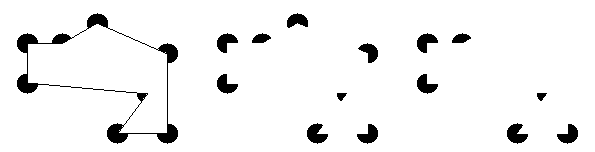
\includegraphics[scale=.5]{images/kaniszapoly.png}
\item[Example]	
For detailed usage example, see:\\ \verb+http://peblblog.blogspot.com/2010/11/kanizsa-shapes.html+
Part of a script using KaniszaPolygon:	
\begin{verbatim}
   #Specify the xy points
   xys <- [[10,10],[10,50],[130,60],[100,100],[150,100],
           [150,20],[80,-10],[45,10]]
    
    #Specify which vertices to show (do all)
    show <- [1,1,1,1,1,1,1,1]
     
    #Make one, showing the line
    x <-  KaniszaPolygon(xys,show,10,fg,bg,1)
    AddObject(x,gWin);   Move(x,200,200)

    #Make a second, not showing the line
    x2 <-  KaniszaPolygon(xys,show,10,fg,bg,0)
    AddObject(x2,gWin);   Move(x2,400,200)

    #Make a third, only showing some vertices:
    x3 <-  KaniszaPolygon(xys,[1,1,1,1,1,0,0,1],10,fg,bg,0)
    AddObject(x3,gWin);  Move(x3,600,200)
        
\end{verbatim}


\item[See Also] \verb+Polygon()+, \verb+KaneszaSquare()+
\end{desc}

\begin{desc}{Name/Symbol}
\item[Name/Symbol]	\verb+KaniszaSquare+

\item[Description]	Creates generic Kanesza Square, one defined only by with ``pac-man'' circles at its vertices:  

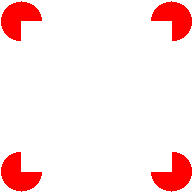
\includegraphics[scale=.5]{images/kaniszasquare.png} 
 

\item[Usage]	
\begin{verbatim}
   KaniszaSquare(<size>, <circ-rad>,<fgcol>, <bgcol>)
\end{verbatim}
KaniszaSquare creates a graphical object that can be added to a window, moved to the proper location, etc.  Parameters specify the size of the square, the size of the vertex circles, and the foreground and background colors.

\item[Example]	
For detailed usage example, see
\verb+http://peblblog.blogspot.com/2010/11/kanizsa-shapes.html+
	
\begin{verbatim}

   gWin <- MakeWindow()
   square <- KaniszaSquare(150,20,MakeColor("red"),
                                  MakeColor("green"))
   AddObject(square,gWin)
   Move(square,200,200)
   Draw()
   WaitForAnyKeyPress()

\end{verbatim}
  


\item[See Also] \verb+Polygon()+, \verb+KaneszaPolygon()+
\end{desc}

\vfill
\newpage
\sect{L}
\vfill


\begin{desc}{Name/Symbol}
\item[Name/Symbol]	\verb+Last()+

\item[Description]	Returns the last item in a list. Provides faster 
		access to the last item of a list than does Nth().

\item[Usage]
\begin{verbatim}
Last(<list>)
\end{verbatim}

\item[Example]
\begin{verbatim}
Last([1,2,3,444])	# == 444
\end{verbatim}

\item[See Also]	\verb+Nth()+, \verb+First()+
\end{desc}




\begin{desc}{Name/Symbol}
\item[Name/Symbol]	\verb+LatinSquare()+

\item[Description]	Quick and dirty latin square, taking on just one
  list argument.

\item[Usage]
\begin{verbatim}
LatinSquare(<list>)
\end{verbatim}

\item[Example]
\begin{verbatim}
Print(LatinSquare([11,12,13,14,15,16]))
# Output:
#[[11, 12, 13, 14, 15, 16]
#, [12, 13, 14, 15, 16, 11]
#, [13, 14, 15, 16, 11, 12]
#, [14, 15, 16, 11, 12, 13]
#, [15, 16, 11, 12, 13, 14]
#, [16, 11, 12, 13, 14, 15]
#]

\end{verbatim}

\item[See Also] \verb+DesignFullCounterBalance()+,
  \verb+DesignBalancedSampling()+, \verb+DesignGrecoLatinSquare()+,
  \verb+DesignLatinSquare()+, \verb+Repeat()+, \verb+RepeatList()+,
  \verb+Shuffle()+

\end{desc}


\begin{desc}{Name/Symbol}
\item[Name/Symbol]	\verb+LaunchFile()+

\item[Description]	Launch a specified file or URI with a platform-specific handler.

\item[Usage]
\begin{verbatim}
LaunchFile("filename")
\end{verbatim}

\item[Example]
Example uses:
\begin{verbatim}

#open google:
LaunchFile("http://google.com")    
#Open a .pbl file with text editor:
LaunchFile("test.pbl")             
#Open a data directory in file manager:
LaunchFile("data\")                
\end{verbatim}

\item[See Also] 
  \verb+SystemCall()+

\end{desc}



\begin{desc}{Name/Symbol}
   
\item[Name/Symbol] \verb+LayoutGrid+

\item[Description]      Creates a grid of x,y points in a range, that are 
spaced in a specified number of rows and columns.  Furthermore, you can specify
whether they are vertical or horizontally laid out.

\item[Usage]       
\verb+LayoutGrid(<xmin>,<xmax>,<ymin>,<ymax>,<culumns>,<rows>,<vertical>)+

\item[Example]

Example PEBL Program using NonoverlapLayout:
\begin{verbatim}
define Start(p)
{
   gWin <- MakeWindow()
   gVideoWidth <- 800
   gVideoHeight <- 300

   lab1 <- EasyLabel("LayoutGrid, horizontal",
                     200,25,gWin,24)
   lab2 <- EasyLabel("LayoutGrid, vertical",
                     600,25,gWin,24)
   nums <- Sequence(1,20,1)
   stim1 <- []
   stim2 <- []

   font <- MakeFont(gPeblBaseFont,0,25,
              MakeColor("black"),MakeColor("white"),0)
   loop(i,nums)
   {
     stim1 <- Append(stim1,MakeLabel(i+"",font))
     stim2 <- Append(stim2,MakeLabel(i+"",font))
    }

  layout1 <- LayoutGrid(50,gVideoWidth/2-50,
                       50,gVideoHeight-50,5,4,0)
  layout2 <- LayoutGrid(gVideoWidth/2+50,gVideoWidth-50,
                       50,gVideoHeight-50,5,4,1)


  ##Now, layout the stuff.

  loop(i,Transpose([stim1,layout1]))
   {	
      obj <- First(i)
      xy <- Second(i)
      AddObject(obj,gWin)
      Move(obj, First(xy),Second(xy))
   }

  loop(i,Transpose([stim2,layout2]))
   {	
      obj <- First(i)
      xy <- Second(i)
      AddObject(obj,gWin)
      Move(obj, First(xy),Second(xy))
   }

  Draw()
  WaitForAnyKeyPress()
}
\end{verbatim}

The output of the above program is shown below.  Even for the left configuration, which is too compact (and which takes a couple seconds to run), the targets are fairly well distributed.
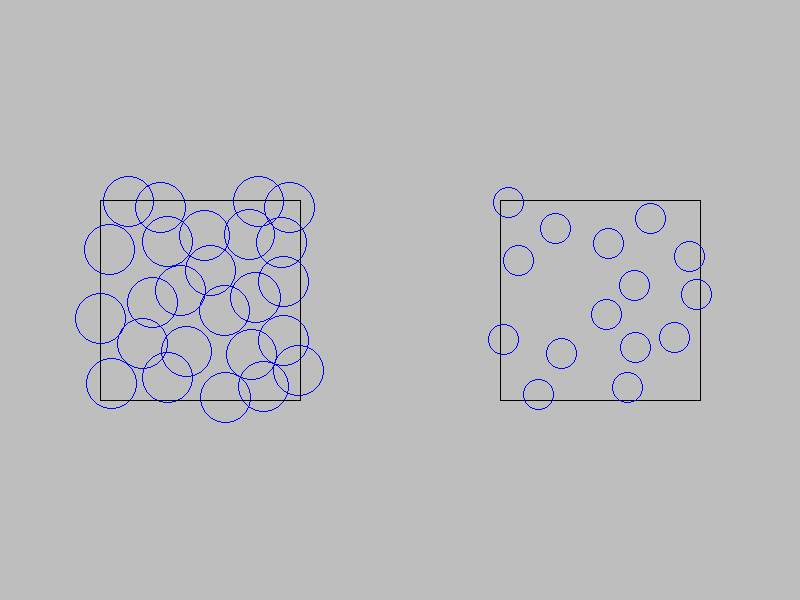
\includegraphics[scale=.35]{images/LayoutGrid.png} 

\item[See Also]     
\verb+NonOverlapLayout()+
\end{desc}



\begin{desc}{Name/Symbol}
\item[Name/Symbol]	\verb+Line()+

\item[Description] Creates a line for graphing at x,y ending at x+dx,
  y+dy.  dx and dy describe the size of the line.  Lines must be added
  to a parent widget before it can be drawn; it may be added to
  widgets other than a base window. Properties of lines may be
  accessed and set later.

\item[Usage]
\begin{verbatim}
Line(<x>, <y>, <dx>, <dy>, <color>)
\end{verbatim}

\item[Example]	
\begin{verbatim}
  l <- Line(30,30,20,20, MakeColor("green")
  AddObject(l, win)
  Draw()

\end{verbatim}
\item[See Also]	\verb+Square()+, \verb+Ellipse()+, \verb+Rectangle()+, \verb+Circle()+
\end{desc}
\begin{desc}{Name/Symbol}
\item[Name/Symbol]	\verb+List()+

\item[Description]	Creates a list of items. Functional version of \verb+[]+.

\item[Usage]
\begin{verbatim}
List(<item1>, <item2>, ....)
\end{verbatim}

\item[Example]
\begin{verbatim}
List(1,2,3,444)		# == [1,2,3,444]
\end{verbatim}

\item[See Also]	\verb+[ ]+, \verb+Merge()+, \verb+Append()+
\end{desc}

\begin{desc}{Name/Symbol}
\item[Name/Symbol]	\verb+ListBy()+

\item[Description]	organizes a list into sublists, based on the
  elements of a second list.  It returns a list of two entities: (1) a
  condition list, describing what values were aggregated across; (2)
  the nested list elements.  The length of each element should be the same.

Together with Match and Filter, ListBy is useful for aggregating data across blocks and conditions for immediate feedback.

\item[Usage]
\begin{verbatim}
ListBy(<list>, <conds>)
\end{verbatim}

\item[Example]
\begin{verbatim}

	a <- Sequence(1,10,1)
    b <- RepeatList([1,2],5)
    x <- ListBy(a,b)
    Print(x)
#[[1, 2],
#  [[1, 3, 5, 7, 9],
#   [2, 4, 6, 8, 10]]
#]

    Print(ListBy(b,a))
#[[1, 2, 3, 4, 5, 6, 7, 8, 9, 10],
# [[1], [2], [1], [2], [1], [2], [1], [2], [1], [2]]]

\end{verbatim}

\item[See Also]	\verb+List()+, \verb+[ ]+, \verb+Merge()+, \verb+Append()+
\end{desc}
 
\begin{desc}{Name/Symbol}
\item[Name/Symbol]	\verb+ListToString()+

\item[Description]	Converts a list of things to a single string

\item[Usage]
\begin{verbatim}
  ListToString(<list>)
\end{verbatim}

\item[Example]
\begin{verbatim}
ListToString([1,2,3,444])		# == "123444"
ListToString(["a","b","c","d","e"])		# == "abcde"

\end{verbatim}

\item[See Also] \verb+SubString+, \verb+StringLength+
\end{desc}

\begin{desc}{Name/Symbol}
\item[Name/Symbol]	\verb+Length()+

\item[Description]	Returns the number of items in a list.

\item[Usage]
\begin{verbatim}
Length(<list>)
\end{verbatim}

\item[Example]
\begin{verbatim}
Length([1,3,55,1515])	# == 4
\end{verbatim}

\item[See Also]	\verb+StringLength()+
\end{desc}

\begin{desc}{Name/Symbol}
\item[Name/Symbol]	\verb+Levels()+

\item[Description]	Returns sorted list of unique elements of a list.

\item[Usage]
\begin{verbatim}
Levels(<list>)
\end{verbatim}

\item[Example]
\begin{verbatim}
Levels([1,3,55,1,5,1,5])	# == [1,3,5,55]
\end{verbatim}

\item[See Also]	\verb+Match()+, \verb+Filter()+, \verb+Sort()+
\end{desc}


\begin{desc}{Name/Symbol}
\item[Name/Symbol]	\verb+LoadAudioFile()+
 
\item[Description] Loads an audio file supported by  the ffmpeg library.  It is nearly identical to
LoadMovie(), but only works for audio files (.ogg, .mp3, .wav, .aiff, .wma, et.).  It creates a movie
object, which can then be played using PlayMovie() or StartPlayback() functions.  Currently,
only supported on Windows and Linux.

The ffmpeg (\verb+http://ffmpeg.org+) library supports a wide range of audio formats,
including most .wav, .mp3, .ogg, .flac, .aiff, .wma, and others.   Currently, there appears to sometimes
be playback problems if the audio stream is not stereo, so be sure to convert your audio to stereo.
Also, there appears to be some problems with .flac data formats.

If you have problems with playback, 
you should verify that your media file loads with another ffmpeg media player.

\item[Usage]		
\begin{verbatim}
LoadAudioFile(audiofile)
\end{verbatim}

\item[Example]	
\begin{verbatim}
   movie <- LoadAudioFile("instuctions.mp3")
   PrintProperties(inst)
   PlayMovie(inst)
   PausePlayback(insnt)
\end{verbatim}

\item[See Also]  \verb+LoadMovie()+, \verb+tPlayMovie()+,\verb+StartPlayback()+ \verb+PausePlayback()+
\end{desc}


\begin{desc}{Name/Symbol}
\item[Name/Symbol]	\verb+LoadMovie()+
 
\item[Description] Loads a movie file using the ffmpeg library.  It creates a movie
object, which can then be played using PlayMovie() or StartPlayback() functions.  Currently,
only supported on Windows and Linux.

The ffmpeg (\verb+http://ffmpeg.org+) library supports a wide range of video and audio formats,
including most .mpg, .avi, .ogg and .mp3 type formats.  Audio-only formats should load
and play with LoadMovie, but another function, LoadAudioFile(), has been created for these,
as they do not need to be added to a window to work.

If you have problems with playback, 
you should verify that your media file loads with another ffmpeg media player.

For technical reasons, a movie MUST be loaded directly onto a window, and not another widget.

\item[Usage]		
\begin{verbatim}
LoadMovie(movie,window, width, height)
\end{verbatim}

\item[Example]	
\begin{verbatim}
   movie <- LoadMovie("movie.avi",gWin,640,480)
   PrintProperties(movie)
   Move(movie,20,20)
   Draw() 
   StartPlayback(movie)
   Wait(500) #Play 500 ms of the movie.
   PausePlayback(movie)
\end{verbatim}

\item[See Also] \verb+LoadAudioFile()+, \verb+LoadMovie()+, \verb+tPlayMovie()+,\verb+StartPlayback()+ \verb+PausePlayback()+
\end{desc}

\begin{desc}{Name/Symbol}
\item[Name/Symbol]	\verb+LoadSound()+

\item[Description]	Loads a soundfile from \verb+<filename>+, 
returning a variable that can be played using the PlayForeground or PlayBackground functions.
\texttt{LoadSound} only loads uncompressed .wav files, but uses a background mixer to play them with fairly low latency.  
In contrast, LoadAudioFile can load many different multimedia files other than .wav, and uses a different audio playback mechanism.  LoadSound
is appropriate for playing stimulus sounds and feedback, whereas LoadAudioFile may be more appropriate for instructions and longer feedback that should be 
encoded efficiently.

When the file gets loaded, it gets automatically transcoded into a stereo 44100-sampling rate audio stream, regardless of its original
playback rate.  We have reports that in some cases, this can cause some problems, especially if a mono file
gets loaded multiple times in an experiment. If you experience playback problems, try converting your audio to 
stereo 44100 hz and see if it helps.

\item[Usage]
\begin{verbatim}
LoadSound(<filename>)
\end{verbatim}

\item[Example]	
\begin{verbatim}
  woof   <- LoadSound("dog.wav")
  PlayBackground(woof)
  Wait(200)
  Stop(woof)
  PlayForeground(woof)
\end{verbatim}

\item[See Also]	
\verb+PlayForeground+, \verb+PlayBackground+, \verb+LoadAudioFile+, \verb+LoadMovie+
\end{desc}


\begin{desc}{Name/Symbol}
\item[Name/Symbol]	\verb+Log10()+

\item[Description]	Log base 10 of \verb+<num>+.

\item[Usage]
\begin{verbatim}
Log10(<num>)
\end{verbatim}

\item[Example]	

\item[See Also]	\verb+Log2()+, \verb+LogN()+, \verb+Ln()+, \verb+Exp()+
\end{desc}

\begin{desc}{Name/Symbol}
\item[Name/Symbol]	\verb+Log2()+

\item[Description]	Log base 2 of \verb+<num>+.

\item[Usage]
\begin{verbatim}
Log2(<num>)
\end{verbatim}

\item[Example]	

\item[See Also]	\verb+Log()+, \verb+LogN()+, \verb+Ln()+, \verb+Exp()+
\end{desc}

\begin{desc}{Name/Symbol}
\item[Name/Symbol]	\verb+LogN()+

\item[Description]	Log base \verb+<base>+ of \verb+<num>+.

\item[Usage]
\begin{verbatim}
LogN(<num>, <base>)
\end{verbatim}

\item[Example]
\begin{verbatim}
LogN(100,10)	# == 2
LogN(256,2)	# == 8
\end{verbatim}

\item[See Also]	\verb+Log()+, \verb+Log2()+, \verb+Ln()+, \verb+Exp()+
\end{desc}

\begin{desc}{Name/Symbol}
\item[Name/Symbol]	\verb+Lowercase()+

\item[Description]	Changes a string to lowercase.  Useful for testing user
		input against a stored value, to ensure case differences
		are not detected.

\item[Usage]
\begin{verbatim}
Lowercase(<string>)
\end{verbatim}

\item[Example]
\begin{verbatim}
Lowercase("POtaTo")	# == "potato"
\end{verbatim}

\item[See Also]	\verb+Uppercase()+
\end{desc}

\begin{desc}{Name/Symbol}
\item[Name/Symbol]	\verb+Ln()+

\item[Description]	Natural log of \verb+<num>+.

\item[Usage]		
\begin{verbatim}
Ln(<num>)
\end{verbatim}

\item[Example]	

\item[See Also]	\verb+Log()+, \verb+Log2()+, \verb+LogN()+, \verb+Exp()+     
\end{desc}





\begin{desc}{Name/Symbol}
\item[Name/Symbol]	\verb+Lookup()+

\item[Description] Returns
element in \verb+<database>+ corresponding to element of
\verb+<keylist>+ that matches \verb+<key>+.

If no match exists, Match returns an empty list.
\item[Usage]		
\begin{verbatim}
Lookup(<key>,<keylist>,<database>)
\end{verbatim}

\item[Example]	

\begin{verbatim}
 keys     <- [1,2,3,4,5]
 database <- ["market","home","roast beef",
              "none","wee wee wee"]
 Print(Lookup(3,keys,database))) 

## Or, do something like this:
  
data  <- [["punky","brewster"],
          ["arnold","jackson"],
          ["richie","cunningham"],
          ["alex","keaton"]]

d2 <- Transpose(data)
key <- First(data)

Print(Lookup("alex", key, data))
##Returns ["alex","keaton"]
\end{verbatim}
\item[See Also]	\verb+Match+
\end{desc}

\begin{desc}{Name/Symbol}
\item[Name/Symbol]	\verb+loop()+

\item[Description]	Loops over elements in a list.  During each iteration, \verb+<counter>+ is bound to each consecutive member of \verb+<list>+.

\item[Usage]		
\begin{verbatim}
loop(<counter>, <list>)
{
 statements
 to
 be	   
 executed
}
\end{verbatim}

\item[Example]	

\item[See Also]	\verb+while()+, \verb+{ }+
\end{desc}

\vfill
\newpage
\sect{M}
\vfill


\begin{desc}{Name/Symbol}
\item[Name/Symbol]	\verb+MakeAttneave()+

\item[Description] Makes a random 'Attneave' figure\footnote{(Collin, C. A., \& Mcmullen, P. A. (2002). Using Matlab to generate  families of similar Attneave shapes. Behavior Research Methods
 Instruments and Computers, 34(1), 55-68.).}. An Attneave figure is a complex polygon that can be used as a
stimulus in a number of situations.  It returns a sequence
of points for use in Polygon().

{\centering

\includegraphics[scale=.5]{images/attneave.png}
}
\\

MakeAttneave uses ConvexHull,  InsertAttneavePointRandom() and
ValidateAttneaveShape(), found in Graphics.pbl.  Override these
to change constraints such as  minimum/maximum side
lengths, angles, complexity, etc.

MakeAttneave uses a sampling-and-rejection scheme to create in-bounds
shapes.  Thus, if you specify impossible or nearly-impossible
constraints, the time necessary to create shapes may be very long or
infinite.

 The arguments to MakeAttneave are:
\begin{itemize}
\item size: size, in pixels, of a circle from which points are
  sampled in a uniform distribution. 
\item numpoints: number of points in the polygon.
\item minangle: smallest angle acceptable (in degrees).
\item maxangle: largest angle acceptable  (in degrees).
\end{itemize}

\item[Usage]
\begin{verbatim}
  MakeAttneave(size,numpoints,minangle,maxangle)
\end{verbatim}

\item[Example]	
\begin{verbatim}
  gWin <- MakeWindow()
  shape <- MakeAttneave(100,5+RandomDiscrete(5),5,170)
  pts <- Transpose(shape)
  poly <- Polygon(200,200,First(pts),Second(pts),
                  MakeColor("blue"),1)
  AddObject(poly,gWin)
  Draw()
  WaitForAnyKeyPress()
\end{verbatim}
\item[See Also]	\verb+MakeImage()+, \verb+Polygon()+, \verb+Square()+
\end{desc}






\begin{desc}{Name/Symbol}
\item[Name/Symbol]	\verb+MakeAudioInputBuffer(<time-in-ms>)+

\item[Description] Creates a sound buffer to use for audio recording or voicekey sound input.  It is currently very simple, allowing only to set the duration.  By default, it record mono at 44100 hz.

\item[Usage]
\begin{verbatim}
MakeAudioInputBuffer(<time-in-ms>)
\end{verbatim}

See number-stroop.pbl in the stroop directory of the test battery for examples.

Note: Version 0.12 seems to have some trouble specifying buffers of different lengths.  5000 seems to work, but others (3500?) may not.
\item[Example]	
\begin{verbatim}

  buffer <- MakeAudioInputBuffer(5000)
  resp0 <-  GetVocalResponseTime(buffer,.35, 200)
  SaveAudioToWaveFile("output.wav",buffer)
  
\end{verbatim}
\item[See Also] 	\verb+GetVocalResponseTime()+, \verb+SaveAudioToWaveFile()+,
\end{desc}


\begin{desc}{Name/Symbol}
\item[Name/Symbol]	\verb+MakeCanvas()+

\item[Description] Makes a canvas object  \verb+<x>+ pixels by
  \verb+y+ pixels, in color \verb+<color>+.

A canvas is an object that other objects can be attached to, and imprinted upon.
When the canvas gets moved, the attached objects move as well. The background of a canvas can be
made invisible by using a color with alpha channel == 0. The Setpixel
and SetPoint functions let you change individual pixels on a canvas,
to enable adding noise, drawing functional images, etc. A canvas gets
'cleared' by calling ResetCanvas(canvas). Any object added to a canvas creates an 'imprint' on the canvas that
remains if the object is moved.  This allows you to use another image
as a paintbrush on the canvas, and lets you to add noise to text.
Because a text label gets re-rendered when its drawn, if you want to
add pixel noise to a stimulus, you can create a label, add it to a
canvas, then add pixel noise to the canvas.

\item[Usage]
\begin{verbatim}
MakeCanvas(<x>, <y>, <color>)
\end{verbatim}

\item[Example]	
\begin{verbatim}
  gWin <- MakeWindow()
  clear <- MakeColor("white")
  clear.alpha <- 0
  #make a transparent canvas:
  x <- MakeCanvas(300,300,clear)  
  AddObject(x,gWin)
  Move(x,300,300)
  img <- MakeImage("pebl.png")
  AddObject(img,x)
  Move(img,100,100)
  Draw(x)          #imprint the image on the canvas
  Move(img,100,200)
  Draw(x)          #imprint the image on the canvas
  Hide(img)

  #draw a line on the canvas
   i <- 10
   red <- MakeColor("red")
  while(i < 200)
   {
     SetPixel(x,20,i,red)
     i <- i + 1
   }
  Draw()
  WaitForAnyKeyPress()
\end{verbatim}
\item[See Also]	\verb+MakeImage()+, \verb+SetPixel()+,
  \verb+MakeGabor()+, \verb+ResetCanvas()+
\end{desc}



\begin{desc}{Name/Symbol}
\item[Name/Symbol]	\verb+MakeColor()+

\item[Description] Makes a color from \verb+<colorname>+ such as
  ``red'', ``green'', and nearly 800 others.  Color names and
  corresponding RGB values can be found in \verb+doc/colors.txt+.

\item[Usage]
\begin{verbatim}
MakeColor(<colorname>)
\end{verbatim}

\item[Example]	

\item[See Also]	\verb+MakeColorRGB()+, \verb+RGBtoHSV()+
\end{desc}

\begin{desc}{Name/Symbol}
\item[Name/Symbol]	\verb+MakeColorRGB()+ 

\item[Description] Makes an RGB color by specifying \verb+<red>+,
  \verb+<green>+, and \verb+<blue>+ values (between 0 and 255).

\item[Usage]		
\begin{verbatim}
MakeColorRGB(<red>, <green>, <blue>)
\end{verbatim}

\item[Example]	

\item[See Also]	\verb+MakeColor()+, \verb+RGBtoHSV()+
\end{desc}


\begin{desc}{Name/Symbol}
\item[Name/Symbol]	\verb+MakeDirectory()+

\item[Description]	Creates a directory with a particular name. It will have no effect of the directory already exists.
\item[Usage]		
\begin{verbatim}
 FileExists(<path>)
\end{verbatim}

\item[Example]	
\begin{verbatim}
 #create data subdirectory + subject-specific directory
 MakeDirectory("data")
 MakeDirectory("data/"+gsubnum)
 filename <- "data/"+gsubnum+"/output.csv"
  
\end{verbatim}

\item[See Also]\verb+GetDirectoryListing()+, \verb+FileExists()+,       \verb+IsDirectory()+,        
   \verb+MakeDirectory()+      

\end{desc}



\begin{desc}{Name/Symbol}
\item[Name/Symbol]	\verb+MakeFont()+

\item[Description]	Makes a font.  The first argument must be a text
  name of a font.  The font can reside anywhere in PEBL's search path,
  which would primarily include the media/fonts directory, and the
  working directory (where the script is saved).
  \begin{itemize}
  \item  style changes from normal to bold/underline, italic.
  \item    fgcolor and bgcolor need to be colors, not just names of colors
  \item  if show-backing is 0, the font gets rendered with an invisible
  \item    background; otherwise with a bgcolor background. (Note: previous to PEBL 0.11, the final argument = 0 rendered the font  with non anti-aliased background, which I can see almost no use for.)
\end{itemize}
\item[Usage]
\begin{verbatim}
MakeFont(<ttf_filename>, <style>, <size>, 
         <fgcolor>, <bgcolor>, <show-backing>)
\end{verbatim}

\item[Example]	
\begin{verbatim}
  font <- MakeFont("Vera.ttf",0,22,MakeColor("black"),
                    MakeColor("white"),1)
\end{verbatim}

\item[See Also]	
\end{desc}


\begin{desc}{Name/Symbol}
\item[Name/Symbol]	\verb+MakeGabor()+

\item[Description]
Creates a greyscale gabor patch, with seven variables:
\begin{itemize}
\item size (in pixels) of square the patch is drawn on
\item freq: frequency of grating (number of wavelengths in size)
\item sd: standard deviation, in pixels, of gaussian window
\item angle: angle of rotation of grating, in radians
\item phase: phase offset of grating (in radians)
\item bglev: number between 0 and 255 indicating background color in greyscale.
\end{itemize}

{
\center
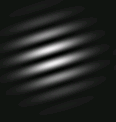
\includegraphics{images/gabor.png}
}
\item[Usage]

\begin{verbatim}
MakeGabor(<size>,<freq>,<sd>, <angle>,<phase>,<bglev>)
\end{verbatim}
MakeGabor creates a canvas that can be used like any image.  It must be added to the window, placed, and drawn to appear.  Typically, it can take several seconds to create a patch of any large size, so it is usually best to create the gabor patches when the test is initiatialized, or save and load images using WritePNG().

Typically, a sd roughly 1/4 to 1/10 the size of size is necessary to avoid vignetting.

\item[Example]	
\begin{verbatim}
   win <- MakeWindow()
   patch <- MakeGabor(80, 0,10,0,0,100)
   AddObject(patch,win)
   Move(patch,200,200)
   Draw()
   
\end{verbatim}

\item[See Also]	
\verb+MakeAttneave()+, \verb+SetPixel()>+, \verb+MakeCanvas()+ 
\end{desc}



\begin{desc}{Name/Symbol}
\item[Name/Symbol]	\verb+MakeImage()+

\item[Description]	Makes an image widget from an image file.
		\texttt{.bmp} formats should be supported; others may be as well.

\item[Usage]		
\begin{verbatim}

MakeImage(<filename>)
\end{verbatim}

\item[Example]	

\item[See Also]	
\end{desc}



\begin{desc}{Name/Symbol}
\item[Name/Symbol]	\verb+MakeLabel()+

\item[Description] Makes a text label for display on-screen. Text will
  be on a single line, and the \verb+Move()+ command centers
  \verb+<text>+ on the specified point.

\item[Usage]
\begin{verbatim}
MakeLabel(<text>, <font>)
\end{verbatim}

\item[Example]	

\item[See Also]	
\end{desc}
\begin{desc}{Name/Symbol}
\item[Name/Symbol]	\verb+MakeNGonPoints()+

\item[Description] 
Creates a set of points that form a regular n-gon.  It can be
transformed with functions like \verb+RotatePoints+, or it can be 
used to create a graphical object with \verb+Polygon+.

Note: \verb+MakeNGonPoints+ returns a list like:
\begin{verbatim}
  [[x1, x2, x3,...],[y1,y2,y3,...]],
\end{verbatim}
while Polygon() takes the X and Y lists independently.

\item[Usage]
\begin{verbatim}
MakeNGonPoints(<radius>, <num_peaks>)
\end{verbatim}

\item[Example]	
\begin{verbatim}
   window <- MakeWindow()
   ngonp <- MakeNGonPoints(50,10)
   ngon <- Polygon(200,200,First(ngonp),Nth(ngonp,2),
                   MakeColor("red"),1)
   AddObject(ngon,window)
   Draw()
\end{verbatim}

\item[See Also]	
\verb+MakeStarPoints+, \verb+Polygon+, \verb+RotatePoints+, \verb+ZoomPoints+
\end{desc}

\begin{desc}{Name/Symbol}
\item[Name/Symbol]	\verb+MakeSineWave()+

\item[Description] 
Creates a sine wave that can be played using the Play() or PlayBackground() functions.  It will create a single-channel sound at 44100 bitrate, 16 bit precision.

\item[Usage]
\begin{verbatim}
MakeSineWave(<duration_in_ms>, <hz>, <amplitude>)
\end{verbatim}
\begin{itemize}
 \item  The first argument specifies how long (in ms) the tone should be.
 \item The second argument specifies the frequency.  Good values range between 100 and 2000.
 \item The third argument specifies the volume.  It should be less than 1.0.
 \end{itemize}
 
\item[Example]	
\begin{verbatim}

   ##Make a sound that is 1000 ms, but just play 300 ms
   sound  <- MakeSineWave(200, 220, 1000)
   PlayBackground(sound)
   Wait(300)
   Stop(sound)

\end{verbatim}

\item[See Also]    	\verb+PlayForeground()+, \verb+PlayBackGround()+, \verb+Stop()+
\end{desc}






\begin{desc}{Name/Symbol}
\item[Name/Symbol]	\verb+MakeStarPoints()+

\item[Description] 
Creates a set of points that form a regular star.  It can be
transformed with functions like \verb+RotatePoints+, or it can be 
used to create a graphical object with \verb+Polygon+.

Note: \verb+MakeStarPoints+ returns a list:
\begin{verbatim}
[[x1, x2, x3,...],[y1,y2,y3,...]],
\end{verbatim}
while \verb+Polygon()+ takes the X and Y lists independently.

\item[Usage]
\begin{verbatim}
MakeStarPoints(<outer_radius>, <inner_radius>,
                <num_peaks>)
\end{verbatim}

\item[Example]	
\begin{verbatim}
   window <- MakeWindow()
   sp <- MakeStarPoints(50,20,10)
   star <- Polygon(200,200,First(sp),Nth(sp,2),
                   MakeColor("red"),1)
   AddObject(star,window)
   Draw()
\end{verbatim}

\item[See Also]	
\verb+MakeNGonPoints+, \verb+Polygon+, \verb+RotatePoints+, \verb+ZoomPoints+
\end{desc}


\begin{desc}{Name/Symbol}
\item[Name/Symbol]	\verb+MakeTextBox()+

\item[Description]	Creates a textbox in which to display text. 
		Textboxes allow multiple lines of text to be rendered;
		automatically breaking the text into lines. 

\item[Usage]
\begin{verbatim}
MakeWindow(<text>,<font>,<width>,<height>)
\end{verbatim}

\item[Example]	
\begin{verbatim}
font <-MakeFont("Vera.ttf", 1, 12, MakeColor("red"), 
MakeColor("green"), 1)
tb <- MakeTextBox("This is the text in the textbox", 
font, 100, 250)
\end{verbatim}

\item[See Also]	\verb+MakeLabel()+, \verb+GetText()+, \verb+SetText()+, \verb+SetCursorPosition()+,
		\verb+GetCursorPosition()+, \verb+SetEditable()+
\end{desc}

\begin{desc}{Name/Symbol}
\item[Name/Symbol]	\verb+MakeWindow()+ 

\item[Description]	Creates a window to display things in.
		Background is specified by \verb+<color>+.

\item[Usage]		
\begin{verbatim}
MakeWindow(<color>)
\end{verbatim}

\item[Example]
\begin{verbatim}	
  win <- MakeWindow()
  gWin <- MakeWindow("white")
\end{verbatim}
    
\item[See Also]	
\end{desc}



\begin{desc}{Name/Symbol}
\item[Name/Symbol]	\verb+Match()+            

\item[Description] Returns a list of 0/1, indicating which elements of  \verb+<list>+ match \verb+<target>+

\item[Usage]		
\begin{verbatim}
Match(<list>,target)
\end{verbatim}

\item[Example]	
\begin{verbatim} 
  x <- [1,2,3,3,2,2,1]
  Print(Match(x,1))  ##== [1,0,0,0,0,0,1]
  Print(Match(x,2))  ##== [0,1,0,0,1,1,0]
  Print( Match(x,3)  ##== [0,0,1,1,0,0,0]

\end{verbatim}

\item[See Also]	\verb+Filter()+, \verb+Subset()+, \verb+Lookup()+
\end{desc}



\begin{desc}{Name/Symbol}
\item[Name/Symbol]	\verb+Max()+            

\item[Description] Returns the largest of \verb+<list>+.

\item[Usage]		
\begin{verbatim}
Max(<list>)
\end{verbatim}

\item[Example]	
\begin{verbatim} 
  c <- [3,4,5,6]
  m <- Max(c) # m == 6
\end{verbatim}

\item[See Also]	\verb+Min()+, \verb+Mean()+, \verb+StDev()+
\end{desc}




\begin{desc}{Name/Symbol}
\item[Name/Symbol]	\verb+Mean()+

\item[Description] 	Returns the mean of the numbers in \verb+<list>+.

\item[Usage]	Mean(\verb+<list-of-numbers>+)	

\item[Example]	
\begin{verbatim} 
  c <- [3,4,5,6]
  m <- Mean(c) # m == 4.5
\end{verbatim}

\item[See Also]	\verb+Median()+, \verb+Quantile()+, \verb+StDev()+, \verb+Min()+, \verb+Max()+
\end{desc}


\begin{desc}{Name/Symbol}
\item[Name/Symbol]	\verb+Median()+

\item[Description]	Returns the median of the numbers in
  \verb+<list>+.  

\item[Usage]	Median(\verb+<list-of-numbers>+)

\item[Example]	
\begin{verbatim} 
  c <- [3,4,5,6,7]
  m <- Median(c) # m == 5
\end{verbatim}
\item[See Also]	\verb+Mean()+, \verb+Quantile()+, \verb+StDev()+, \verb+Min()+, \verb+Max()+
\end{desc}

\begin{desc}{Name/Symbol}
\item[Name/Symbol]	\verb+Merge()+

\item[Description]	Combines two lists, \verb+<lista>+ and \verb+<listb>+, into a single list.

\item[Usage]		
\begin{verbatim}
Merge(<lista>,<listb>)
\end{verbatim}

\item[Example]	
\begin{verbatim}
Merge([1,2,3],[8,9]) 	# == [1,2,3,8,9]
\end{verbatim}

\item[See Also]	\verb+[ ]+, \verb+Append()+, \verb+List()+
\end{desc}


\begin{desc}{Name/Symbol}
\item[Name/Symbol]	\verb+MessageBox()+

\item[Description]	Hides what is on the screen and presents a textbox with
  specified message, with a button to click at the bottom to continue.


\item[Usage]		
\begin{verbatim}
MessageBox(<message>,<window>)
\end{verbatim}

\item[Example]	
\begin{verbatim}
 gWin <- MakeWindow()
 MessageBox("Click below to begin.",gWin)


\end{verbatim}

\item[See Also]	\verb+GetEasyInput+, \verb+EasyTextBox+
\end{desc}



\begin{desc}{Name/Symbol}
\item[Name/Symbol]	\verb+Min()+

\item[Description]	Returns the `smallest' element of a list.

\item[Usage]	
\begin{verbatim}
Min(<list>)
\end{verbatim}

\item[Example]	
\begin{verbatim}
  c <- [3,4,5,6]
  m <-  Min(c) # == 3
\end{verbatim}

\item[See Also]	\verb+Max()+
\end{desc}

\begin{desc}{Name/Symbol}
\item[Name/Symbol]	\verb+Mod()+

\item[Description]	Returns \verb+<num>+, \verb+<mod>+, or remainder of \verb+<num>/<mod>+

\item[Usage]		
\begin{verbatim}
Mod( <num> <mod>)
\end{verbatim}

\item[Example]	
\begin{verbatim}
Mod(34, 10)	# == 4
Mod(3, 10)	# == 3
\end{verbatim}

\item[See Also]	\verb+Div()+
\end{desc}

\begin{desc}{Name/Symbol}
\item[Name/Symbol]	\verb+Move()+

\item[Description]	Moves an object to a specified location.  
		Images and Labels are moved according to their center; 
		TextBoxes are moved according to their upper left corner.

\item[Usage]
\begin{verbatim}
Move(<object>, <x>, <y>)
\end{verbatim}

\item[Example]	
\begin{verbatim}
Move(label, 33, 100)
\end{verbatim}

\item[See Also]	\verb+MoveCorner()+, \verb+MoveCenter()+, \verb+.X+ and \verb+.Y+ properties.
\end{desc}
\begin{desc}{Name/Symbol}
\item[Name/Symbol]	\verb+MoveCenter()+

\item[Description]	Moves a TextBox to a specified location
		according to its center, instead of its upper left corner.

\item[Usage]
\begin{verbatim}
MoveCenter(<object>, <x>, <y>)
\end{verbatim}

\item[Example]	
\begin{verbatim}
MoveCenter(TextBox, 33, 100)
\end{verbatim}

\item[See Also]	\verb+Move()+, \verb+MoveCenter()+, \verb+.X+ and \verb+.Y+ properties
\end{desc}

\begin{desc}{Name/Symbol}
\item[Name/Symbol]	\verb+MoveCorner()+

\item[Description]	Moves a label or image to a specified location
		according to its upper left corner, instead of its center. 

\item[Usage]
\begin{verbatim}
MoveCorner(<object>, <x>, <y>)
\end{verbatim}

\item[Example]	
\begin{verbatim}
MoveCorner(label, 33, 100)
\end{verbatim}

\item[See Also]	\verb+Move()+, \verb+MoveCenter()+, \verb+.X+ and \verb+.Y+ properties
\end{desc}



\begin{desc}{Name/Symbol}
   
\item[Name/Symbol] \verb+NonOverlapLayout+

\item[Description]        Creates a set of num points in a xy range, that have a (soft) minimum tolerance of 'tol' between points.  That is, to the extent possible, the returned points will have a minumum distance between them of \verb+<tol>+.  This may not be possible or be very difficult, and so after a limited number of attempts (by default, 100), the algorithm will return the current configuration, which may have some violations of the minimum tolerance rule, but it will usually be fairly good.  

The algorithm works by initializing with a random set of points, then computing a pairwise distance matrix between all points, finding the closest two points, and resampling one of them until its minumum distance is larger than the current.  Thus, each internal iteration uniformly improves (or keeps the configuration the same), and the worst points are reconfigured first, so that even if a configuration that does not satisfy the constraints, it will usually be very close.

Internally, the function (located in pebl-lib/Graphics.pbl) has a variable that controls how many steps are taken, called ``limit'', which is set to 100.  For very compacted or very large iterations, this limit can be increased by editing the file or making a copy of the function.  

The function usually returns fairly quickly, so it can often be used real-time between trials.  However, for complex enough configurations, it can take on the order of seconds; furthermore, more  complex configurations might take longer than less complex configurations, which could represent a potential confound (if more complex stimuli have longer ISIs).  Users should thus consider creating the configurations when the test is initialized, or created prior to the study and then saved out to a file for later use.


\newpage

\item[Usage]       
\verb+NonOverlapLayout(<xmin>,<xmax>,<ymin>,<ymax>,<tol>,<num>)+

\item[Example]

Example PEBL Program using NonoverlapLayout:
\begin{verbatim}
define Start(p)
 {
   win <- MakeWindow()  
   ## Make 25 points in a square in the middle 
   ## of the screen, a minimum of 50 pixels apart.  
   ## This is too compact, but it will be OK.

   points <- NonOverlapLayout(100,300,200,400,50,25)
   circs <- []
   ##This should non-overlapping circles of radius 25
   loop(i,points)
    {
       tmp <- Circle(First(i),Second(i),25,
                     MakeColor("blue"),0) 
       AddObject(tmp,win)
       circs <- Append(circs,tmp)
    }


   rect1 <- Square(200,300,200,MakeColor("black"),0)
   rect2 <- Square(600,300,200,MakeColor("black"),0)

   AddObject(rect1,win)
   AddObject(rect2,win)
   ##Reduce the tolerance: this one should be bettter
   points <- NonOverlapLayout(500,700,200,400,50,15)


   ##This should non-overlapping circles of radius 15
   loop(i,points)
    {
       tmp <- Circle(First(i),Second(i),
                     15,MakeColor("blue"),0) 
       AddObject(tmp,win)
	   circs <- Append(circs,tmp)
    }
   Draw()
   WaitForAnyKeyPress()

}
\end{verbatim}
\clearpage
The output of the above program is shown below.  Even for the left configuration, which is too compact (and which takes a couple seconds to run), the targets are fairly well distributed.
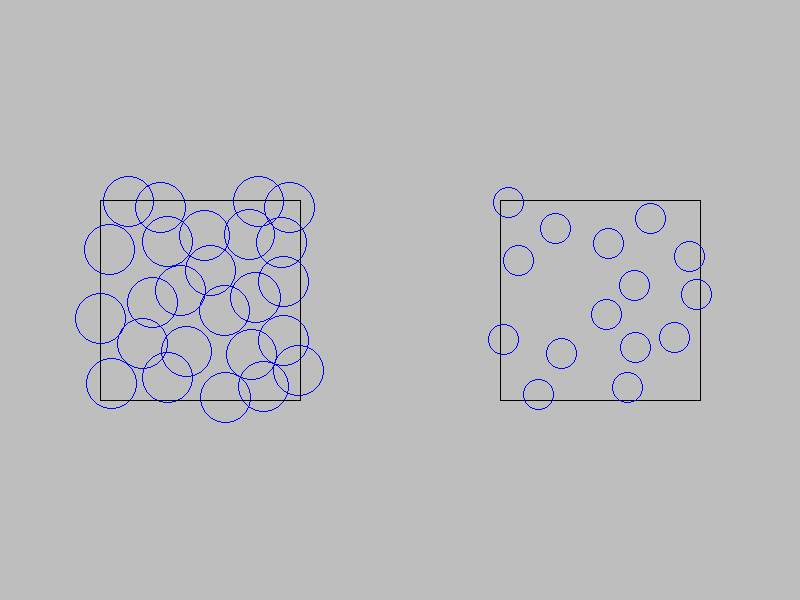
\includegraphics[scale=.35]{images/nonoverlap.png} 


\item[See Also]     
\verb+LayoutGrid()+
\end{desc}





\begin{desc}{Name/Symbol}
\item[Name/Symbol]	\verb+not+

\item[Description]	Logical not

\item[Usage]		

\item[Example]	

\item[See Also]	\verb+and+, \verb+or+
\end{desc}

\vfill
\newpage
\sect{N}
\vfill


\begin{desc}{Name/Symbol}
\item[Name/Symbol]	\verb+NormalDensity()+

\item[Description]	Computes density of normal standard distribution
\item[Usage]
\begin{verbatim}
NormalDensity(<x>)
\end{verbatim}

\item[Example]	
\begin{verbatim}


  Print(NormalDensity(-100))     # 1.8391e-2171
  Print(NormalDensity(-2.32635)) #5.97
  Print(NormalDensity(0))        #0.398942
  Print(NormalDensity(1.28155))  #.90687
  Print(NormalDensity(1000))     #inf

\end{verbatim}

\item[See Also]	\verb+RandomNormal()+, \verb+CumNormInv()+ 
\end{desc}



\begin{desc}{Name/Symbol}
\item[Name/Symbol]	\verb+Nth()+

\item[Description]	Extracts the Nth item from a list.  Indexes from 1 upwards.
		\verb+Last()+ provides faster access than \verb+Nth()+ to the end of a list, 
		which must walk along the list to the desired position.

\item[Usage]
\begin{verbatim}
Nth(<list>, <index>)
\end{verbatim}

\item[Example]	
\begin{verbatim}
a <- ["a","b","c","d"]
Print(Nth(a,3)) 		# == 'c'
\end{verbatim}

\item[See Also]	\verb+First()+, \verb+Last()+ 
\end{desc}

\begin{desc}{Name/Symbol}
\item[Name/Symbol]	\verb+NthRoot()+

\item[Description]	\verb+<num>+ to the power of  1/\verb+<root>+.

\item[Usage]		
\begin{verbatim}
NthRoot(<num>, <root>)
\end{verbatim}

\item[Example]	

\item[See Also]	
\end{desc}

\vfill
\newpage
\sect{O}
\vfill


\begin{desc}{Name/Symbol}
\item[Name/Symbol] \verb+OpenCOMPort+ 

\item[Description]  
  This opens a COM/Serial port
\item[Usage]       
     \verb+OpenCOMPort(<portnum>,<baud>)+ 

\item[Example]

\item[See Also]
\verb+COMPortGetByte+, \verb+COMPortSendByte+, \verb+OpenPPort+, \verb+SetPPortMode+, \verb+GetPPortMode+ 
\end{desc} 




\begin{desc}{Name/Symbol}
\item[Name/Symbol] \verb+OpenJoystick+ 

\item[Description]  
  This opens an available joystick, as specified by its index.  The returned object can then be used in to access the state of the joystick.  It takes an integer argument, and for the most part, if you have a single joystick attached to your system, you will use OpenJoystick(1).  If you want to use a second joystick, use OpenJoystick(2), and so on.
  
  \item[Usage]          \verb+OpenJoystick()+ 

\item[Example]
See joysticktest.pbl in the demo\ directory

\item[See Also]
GetNumJoysticks(), OpenJoystick(), GetNumJoystickAxes()
GetNumJoystickBalls(), GetNumJoystickButtons(), GetNumJoystickHats()
GetJoystickAxisState(), GetJoystickHatState(), GetJoystickButtonState()
\end{desc} 


\begin{desc}{Name/Symbol}
\item[Name/Symbol]	\verb+OpenNetworkListener()+

\item[Description] Creates a network object that listens on a particular port, and is able to accept incoming connections. You can the nuse \verb+CheckForNetworkConnections+ to accept incoming connections.  
This is an alternative to the \verb+WaitForNetworkConnection+ function that allows more flexibility (and allows updating the during waiting for the connection).

\item[Usage]
\begin{verbatim}
net <- OpennetworkListener(port)
\end{verbatim}

\item[Example]	
\begin{verbatim}
  network <-      OpenNetworkListener(4444) 
  time <- GetTime()
  while(not connected and (GetTime() < time + 5000))
   {
      connected <- CheckForNetwokConnection(network) 
   }

\end{verbatim}
\item[See Also]	\verb+CheckForNetworkConnection()+, \verb+Getdata()+, \verb+WaitForNetworkConnection()+, \verb+CloseNetwork()+
\end{desc}


\begin{desc}{Name/Symbol}
\item[Name/Symbol]	\verb+or+                   

\item[Description]	Logical or

\item[Usage]		

\item[Example]	

\item[See Also]	\verb+and+, \verb+not+
\end{desc}



\begin{desc}{Name/Symbol}
\item[Name/Symbol] \verb+OpenPPort+ 

\item[Description]  
  Opens a Parallel  port, returning an object that can be used for parallel port communications.
\item[Usage]       
     \verb+OpenPPort(<name>)+ 
 The <name> argument can be one of: "LPT1", "LPT2", and "LPTX".  Most likely, a parallel port will be configured to 
LPT1, but other configurations are sometimes possible. 
\item[Example]

\item[See Also]
\verb+COMPortGetByte+, \verb+COMPortSendByte+, \verb+OpenCOMPort+, \verb+SetPPortMode+, \verb+GetPPortMode+ 
\end{desc} 





\begin{desc}{Name/Symbol}
\item[Name/Symbol]	\verb+Order()+

\item[Description]	Returns a list of indices describing the order of values by position, from min to max. 

\item[Usage]
\begin{verbatim}
		Order(<list-of-numbers>)
\end{verbatim}

\item[Example]	
\begin{verbatim}
	n <- [33,12,1,5,9]
  	o <- Order(n)
    Print(o) #should print [3,4,5,2,1]
\end{verbatim}

\item[See Also]	\verb+Rank()+
\end{desc}

\vfill
\newpage
\sect{P}
\vfill

\begin{desc}{Name/Symbol}
\item[Name/Symbol]	\verb+PausePlayback()+
 
\item[Description] Pauses a playing movie or audio stream.  This is used for 
movies whose playback was initiated using STartPlayback, which then ran as
background threads during a Wait() function. 

\item[Usage]		
\begin{verbatim}
PausePlayBack(movie)
\end{verbatim}

\item[Example]	
\begin{verbatim}
   movie <- LoadMovie("movie.avi",gWin,640,480)
   PrintProperties(movie)
   Move(movie,20,20)
   Draw() 
   StartPlayback(movie)
   Wait(500) #Play 500 ms of the movie.
   PausePlayback(movie)
   Wait(500)
   
\end{verbatim}

\item[See Also] \verb+LoadAudioFile()+, \verb+LoadMovie()+, \verb+tPlayMovie()+, \verb+StartPlayback()+
\end{desc}




\begin{desc}{Name/Symbol}
\item[Name/Symbol]	\verb+PlayForeground()+  

\item[Description]	Plays the sound `in the foreground'; 
		does not return until the sound is complete.

\item[Usage]		
\begin{verbatim}
PlayForeground(<sound>)
\end{verbatim}

\item[Example]	
\begin{verbatim}
   sound  <- MakeSineWave(200, 220, 1000)
   PlayForeground(sound)
\end{verbatim}
\item[See Also]	\verb+PlayBackground()+, \verb+Stop()+
\end{desc}

\begin{desc}{Name/Symbol}
\item[Name/Symbol]	\verb+PlayBackground()+
 
\item[Description]	Plays the sound `in the background', returning immediately.

\item[Usage]		
\begin{verbatim}
PlayBackground(<sound>)
\end{verbatim}

\item[Example]	
\begin{verbatim}
   sound  <- MakeSineWave(200, 220, 1000)
   PlayBackground(sound)
   Wait(300)
   Stop(sound)
\end{verbatim}

\item[See Also]	\verb+PlayForeground()+, \verb+Stop()+
\end{desc}


\begin{desc}{Name/Symbol}
\item[Name/Symbol]	\verb+PlayMovie()+
 
\item[Description]	Plays the movie (or other multimedia file) loaded via
either the LoadMovie or LoadAudioFile function.  Note that this functionality uses a 
different underlying system than the sound playing functions PlayBackground and PlayForeground,
and they are not interchangeable.

\item[Usage]		
\begin{verbatim}
PlayMovie(movie)
\end{verbatim}

\item[Example]	
\begin{verbatim}
   movie <- LoadMovie("movie.avi",gWin,640,480)
   PrintProperties(movie)
   Move(movie,20,20)
   movie.volume <- .1
   status <- EasyLabel("Demo Movie Player",300,25,gWin,22)    
   Draw()
   PlayMovie(movie)
\end{verbatim}

\item[See Also] \verb+LoadAudioFile()+, \verb+LoadMovie()+, \verb+StartPlayback()+, \verb+PausePlayback()+
\end{desc}




\begin{desc}{Name/Symbol}
\item[Name/Symbol]  	\verb+Plus+ 

\item[Description] Creates a polygon in the shape of a
 plus sign. Arguments include position in window.
\begin{itemize}
\item \verb+<x>+ and \verb+<y>+ is the position of the center
\item \verb+<size>+ or the size of the plus sign in pixels
\item \verb+<width>+ thickness of the plus
\item \verb+<color>+ is a color object (not just the name)
\end{itemize}

Like other drawn objects, the plus must then be added to the window
to appear.

\item[Usage]		
\begin{verbatim}
 Plus(x,y,size,width,color)
\end{verbatim}

\item[Example]	
\begin{verbatim}
  win <- MakeWindow()
  p1 <- Plus(100,100,80,15,MakeColor("red"))
  AddObject(p1,win)
  Draw()
\end{verbatim}

\item[See Also]   
\verb+BlockE()+, \verb+Polygon()+, \verb+MakeStarPoints()+,
\verb+MakeNGonPoints()+
\end{desc}

\begin{desc}{Name/Symbol}
\item[Name/Symbol]  	\verb+Polygon+ 

\item[Description] Creates a polygon in the shape of the points
specified by \verb+<xpoints>+, \verb+<ypoints>+. The lists \verb+<xpoints>+ and
\verb+<ypoints>+ are adjusted by  \verb+<x>+ and \verb+<y>+, so they
should be relative to 0, not the location you want the points to be at.

Like other drawn objects, the polygon must then be added to the window
to appear.

\item[Usage]		
\begin{verbatim}
  Polygon(<x>,<y>,<xpoints>,<ypoints>,
          <color>,<filled>)
\end{verbatim}

\item[Example]	
\begin{verbatim}
  win <- MakeWindow()
   #This makes a T
   xpoints <- [-10,10,10,20,20,-20,-20,-10]
   ypoints <- [-20,-20,40,40,50,50,40,40]
  p1 <-    Polygon(100,100,xpoints, ypoints,
                   MakeColor("black"),1)
  AddObject(p1,win)
  Draw()
\end{verbatim}

\item[See Also]   
\verb+BlockE()+, \verb+Bezier()+, \verb+MakeStarPoints()+,
\verb+MakeNGonPoints()+
\end{desc}

\begin{desc}{Name/Symbol}
\item[Name/Symbol]	\verb+Pow()+ 

\item[Description]	Raises or lowers \verb+<num>+ to the power of \verb+<pow>+.

\item[Usage]		
\begin{verbatim}
Pow(<num>, <pow>)
\end{verbatim}

\item[Example]	
\begin{verbatim}
Pow(2,6)	# == 64
Pow(5,0)	# == 1
\end{verbatim}

\item[See Also]     
\end{desc}

\begin{desc}{Name/Symbol}
\item[Name/Symbol]	\verb+Print()+

\item[Description]	Prints \verb+<value>+ to stdout (the console [Linux] or the file \texttt{stdout.txt} [Windows]), and then appends a newline afterwards.

\item[Usage]		
\begin{verbatim}
Print(<value>)
\end{verbatim}

\item[Example]	
\begin{verbatim}
  Print("hello world")
  Print(33 + 43)
  x <-Print("Once")

\end{verbatim}
\item[See Also]	\verb+Print_()+, \verb+FilePrint()+
\end{desc}
\begin{desc}{Name/Symbol}
\item[Name/Symbol]	\verb+PrintProperties()+

\item[Description]	Prints .properties/values for any complex object.
  These include textboxes, fonts, colors, images, shapes, etc. Mostly
  useful as a debugging tool.

\item[Usage]		
\begin{verbatim}
PrintProperties(<object>)
\end{verbatim}

\item[Example]	
\begin{verbatim}


   win <- MakeWindow()
   tb <- EasyTextbox("one",20,20,win,22,400,80)
   PrintProperties(tb)

##Output:
----------
[CURSORPOS]: 0
[EDITABLE]: 0
[HEIGHT]: 80
[ROTATION]: 0
[TEXT]: one
[VISIBLE]: 1
[WIDTH]: 400
[X]: 20
[Y]: 20
[ZOOMX]: 1
[ZOOMY]: 1
----------

\end{verbatim}
\item[See Also]	\verb+Print()+
\end{desc}


\begin{desc}{Name/Symbol}
\item[Name/Symbol]	\verb+Print_()+

\item[Description]	Prints \verb+<value>+ to stdout; doesn't append a newline afterwards.

\item[Usage]		
\begin{verbatim}
Print_(<value>)
\end{verbatim}

\item[Example]	
\begin{verbatim}
Print_("This line")
Print_(" ")
Print_("and")
Print_(" ")
Print("Another line")
# prints out: 'This line and Another line'
\end{verbatim}

\item[See Also]	\verb+Print()+, \verb+FilePrint()+
\end{desc}


\begin{desc}{Name/Symbol}
\item[Name/Symbol]	\verb+PrintList()+

\item[Description]	Prints a list, without the ','s or []
  characters. Puts a carriage return at the end.  Returns a string
  that was printed.  If a list contains other lists, the printing will
  wrap multiple lines and the internal lists will be printed as
  normal.  To avoid this, try PrintList(Flatten(list)).

\item[Usage]
\begin{verbatim}
PrintList( <list>)
\end{verbatim}

\item[Example]
\begin{verbatim}
PrintList( [1,2,3,4,5,5,5])
##
##  Produces:
##1 2 3 4 5 5 5
PrintList([[1,2],[3,4],[5,6]])
#Produces:
# [1,2]
#,[3,4]
#,[5,6]

PrintList(Flatten([[1,2],[3,4],[5,6]]))
#Produces:
# 1 2 3 4 5 6

\end{verbatim}

\item[See Also]	\verb+Print()+, \verb+Print_()+, \verb+FilePrint()+, \verb+FilePrint_()+, \verb+FilePrintList()+,
\end{desc}

\begin{desc}{Name/Symbol}
\item[Name/Symbol]  	\verb+PushOnEnd+
  
\item[Description]  	Pushes an item onto the end of a list, modifying the list itself.

Note: \texttt{PushOnEnd} is a more efficient replacement for \texttt{Append()}. Unlike \texttt{Append}, it will modify the original list as a side effect, so the following works:

\begin{verbatim}
  PushOnEnd(list, item)
\end{verbatim}
There is no need to set the original list to the result of PushOnEnd, like you must do with Append.  However, it does in fact work, and incurs only a slight overhead, so that Append can often be replaced with PushOnEnd without worry.
\begin{verbatim}
 list <-  PushOnEnd(list, item)
\end{verbatim}

\item[Usage] 
\begin{verbatim}
PushOnEnd(<list>, <item>)
\end{verbatim}

\item[Example]
\begin{verbatim}
list <- Sequence(1,5,1)
double  <- []
loop(i, list)
{
  PushOnEnd(double, [i,i])
}
Print(double)
# Produces [[1,1],[2,2],[3,3],[4,4],[5,5]]

\end{verbatim}

\item[See Also]  \verb+SetElement()+ \verb+List()+, \verb+[ ]+, \verb+Merge()+, \verb+PushOnEnd+
\end{desc}


\vfill
\newpage
\sect{Q}
\vfill


\begin{desc}{Name/Symbol}
\item[Name/Symbol]	\verb+Quantile()+

\item[Description]	Returns the \verb+<num>+ quantile of
		the numbers in \verb+<list>+. \verb+<num>+ should be  between
        0 and 100

\item[Usage]		
\begin{verbatim}
Quantile(<list>, <num>)
\end{verbatim}

\item[Example]	
 \begin{verbatim}
      ##Find 75th percentile to use as a threshold.
      thresh <- Quantile(rts,75) 
 \end{verbatim}
\item[See Also]	\verb+StDev()+, \verb+Median()+, \verb+Mean()+, \verb+Max()+, \verb+Min()+
\end{desc}

\vfill
\newpage
\sect{R}
\vfill


\begin{desc}{Name/Symbol}
\item[Name/Symbol] 	\verb+RadToDeg()+ 

\item[Description] 	Converts \verb+<rad>+ radians to degrees.

\item[Usage]		
\begin{verbatim}
RadToDeg( <rad>)			 
\end{verbatim}

\item[Example]	

\item[See Also]     	\verb+DegToRad()+, \verb+Tan()+, \verb+Cos()+, \verb+Sin()+, \verb+ATan()+, \verb+ASin()+, \verb+ACos()+
\end{desc}


\begin{desc}{Name/Symbol}
\item[Name/Symbol]	\verb+Random()+

\item[Description]	Returns a random number between 0 and 1.

\item[Usage]
\begin{verbatim}
Random()
\end{verbatim}

\item[Example]
\begin{verbatim}
a <- Random()
\end{verbatim}

\item[See Also]		\verb+Random()+, \verb+RandomBernoulli()+, \verb+RandomBinomial()+, \verb+RandomDiscrete()+, \verb+RandomExponential()+, \verb+RandomLogistic()+, \verb+RandomLogNormal()+, \verb+RandomNormal()+, \verb+RandomUniform()+, \verb+RandomizeTimer()+, \verb+SeedRNG()+
\end{desc}

\begin{desc}{Name/Symbol}
\item[Name/Symbol]	\verb+RandomBernoulli()+

\item[Description]	Returns 0 with probability \verb+(1-<p>)+ and 1 with probability \verb+<p>+.

\item[Usage]		
\begin{verbatim}
RandomBernoulli(<p>)
\end{verbatim}

\item[Example]	
\begin{verbatim}
RandomBernoulli(.3)
\end{verbatim}

\item[See Also] \verb+Random()+, \verb+RandomBernoulli()+,
  \verb+RandomBinomial+, \verb+RandomDiscrete()+,
  \verb+RandomExponential()+, \verb+RandomLogistic()+,
  \verb+RandomLogNormal()+, \verb+RandomNormal()+,
  \verb+RandomUniform()+, \verb+RandomizeTimer()+, \verb+SeedRNG()+
\end{desc}

\begin{desc}{Name/Symbol}
\item[Name/Symbol]	\verb+RandomBinomial+

\item[Description] Returns a random number according to the Binomial
  distribution with probability \verb+<p>+ and repetitions \verb+<n>+,
  i.e., the number of \verb+<p>+ Bernoulli trials that succeed out of
  \verb+<n>+ attempts.

\item[Usage]		
\begin{verbatim}
RandomBinomial(<p> <n>)  
\end{verbatim}

\item[Example]	
\begin{verbatim}
RandomBinomial(.3, 10) # returns number from 0 to 10
\end{verbatim}

\item[See Also]	\verb+Random()+, \verb+RandomBernoulli()+, \verb+RandomBinomial+,
		\verb+RandomDiscrete()+, \verb+RandomExponential()+, \verb+RandomLogistic()+,
		\verb+RandomLogNormal()+, \verb+RandomNormal()+, \verb+RandomUniform()+,    
		\verb+RandomizeTimer()+, \verb+SeedRNG()+    
\end{desc}

\begin{desc}{Name/Symbol}
\item[Name/Symbol]	\verb+RandomDiscrete()+

\item[Description]	Returns a random integer between 1 and the argument 
		(inclusive), each with equal probability.  If the argument is 
		a floating-point value, it will be truncated down; if it is 
		less than 1, it will return 1, and possibly a warning message. 

\item[Usage]		
\begin{verbatim}
RandomDiscrete(<num>)
\end{verbatim}
         
\item[Example]	
\begin{verbatim}
 # Returns a random integer between 1 and 30:
RandomDiscrete(30)
\end{verbatim}

\item[See Also]	\verb+Random()+, \verb+RandomBernoulli()+, \verb+RandomBinomial+, 
		\verb+RandomDiscrete()+, \verb+RandomExponential()+, \verb+RandomLogistic()+,
		\verb+RandomLogNormal()+, \verb+RandomNormal()+, \verb+RandomUniform()+,
		\verb+RandomizeTimer()+, \verb+SeedRNG()+    
\end{desc}

\begin{desc}{Name/Symbol}
\item[Name/Symbol]	\verb+RandomExponential()+

\item[Description]	Returns a random number according to exponential 
		distribution with mean \verb+<mean>+ (or decay 1/mean).

\item[Usage]		
\begin{verbatim}
RandomExponential(<mean>)
\end{verbatim}

\item[Example]	
\begin{verbatim}
RandomExponential(100)
\end{verbatim}

\item[See Also]	\verb+Random()+, \verb+RandomBernoulli()+, \verb+RandomBinomial+,
		\verb+RandomDiscrete()+, \verb+RandomLogistic()+, \verb+RandomLogNormal()+, 
		\verb+RandomNormal()+, \verb+RandomUniform()+, \verb+RandomizeTimer+, \verb+SeedRNG()+
\end{desc}




\begin{desc}{Name/Symbol}
\item[Name/Symbol]	\verb+RandomizeTimer()+

\item[Description]	Seeds the RNG with the current time.

\item[Usage]
\begin{verbatim}
RandomizeTimer()
\end{verbatim}

\item[Example]	
\begin{verbatim}
RandomizeTimer()
x <- Random()
\end{verbatim}
	     
\item[See Also]	\verb+Random()+, \verb+RandomBernoulli()+, \verb+RandomBinomial+,
		\verb+RandomDiscrete()+, \verb+RandomExponential()+, \verb+RandomLogistic()+,
		\verb+RandomLogNormal()+, \verb+RandomNormal()+, \verb+RandomUniform()+, \verb+SeedRNG()+
\end{desc}

\begin{desc}{Name/Symbol}
\item[Name/Symbol]	\verb+RandomLogistic()+  

\item[Description]	Returns a random number according to the logistic distribution 
		with parameter \verb+<p>+: f(x) = exp(x)/(1+exp(x))

\item[Usage]		
\begin{verbatim}
RandomLogistic(<p>)
\end{verbatim}

\item[Example]	RandomLogistic(.3)

\item[See Also]	\verb+Random()+, \verb+RandomBernoulli()+, \verb+RandomBinomial+, 
		\verb+RandomDiscrete()+, \verb+RandomExponential()+, \verb+RandomLogNormal()+, 
		\verb+RandomNormal()+, \verb+RandomUniform()+, \verb+RandomizeTimer+, \verb+SeedRNG()+
\end{desc}

\begin{desc}{Name/Symbol}
\item[Name/Symbol] 	\verb+RandomLogNormal()+

\item[Description]  	Returns a random number according to the log-normal 
		distribution with parameters \verb+<median>+ and \verb+<spread>+. Generated 
		by calculating $median \verb!*! exp(spread \verb!*! RandomNormal(0,1))$. 
		\verb+<spread>+ is a shape parameter, and only affects the variance 
		as a function of the median; similar to the coefficient of 
		variation.  A value near 0 is a sharp distribution (.1-.3), 
		larger values are more spread out; values greater than 2 make 
		little difference in the shape.

\item[Usage]
\begin{verbatim}
RandomLogNormal(<median>, <spread>)
\end{verbatim}

\item[Example]      	
\begin{verbatim}
RandomLogNormal(5000, .1)
\end{verbatim}

\item[See Also]	\verb+Random()+, \verb+RandomBernoulli()+, \verb+RandomBinomial+, 
		\verb+RandomDiscrete()+, \verb+RandomExponential()+, \verb+RandomLogistic()+,
		\verb+RandomNormal()+, \verb+RandomUniform()+, \verb+RandomizeTimer+, \verb+SeedRNG()+
\end{desc}

\begin{desc}{Name/Symbol}
\item[Name/Symbol] 	\verb+RandomNormal()+

\item[Description] 	Returns a random number according to the standard
             	normal distribution with \verb+<mean>+ and \verb+<stdev>+.

\item[Usage]       	
\begin{verbatim}
RandomNormal(<mean>, <stdev>)
\end{verbatim}

\item[Example]	

\item[See Also]	\verb+Random()+, \verb+RandomBernoulli()+, \verb+RandomBinomial+,
		\verb+RandomDiscrete()+, \verb+RandomExponential()+, \verb+RandomLogistic()+, 
		\verb+RandomLogNormal()+, \verb+RandomUniform()+, \verb+RandomizeTimer+, \verb+SeedRNG()+
\end{desc}

\begin{desc}{Name/Symbol}
\item[Name/Symbol]	\verb+RandomUniform()+

\item[Description]	Returns a random floating-point number between 0 and \verb+<num>+.

\item[Usage]		
\begin{verbatim}
RandomUniform(<num>)
\end{verbatim}

\item[Example]	

\item[See Also] \verb+Random()+, \verb+RandomBernoulli()+,
  \verb+RandomBinomial+, \verb+RandomDiscrete()+,
  \verb+RandomExponential()+, \verb+RandomLogistic()+,
  \verb+RandomLogNormal()+, \verb+RandomNormal()+, \verb+RandomizeTimer()+,
  \verb+SeedRNG()+
\end{desc}


\begin{desc}{Name/Symbol}
\item[Name/Symbol]	\verb+Rank()+

\item[Description]	Returns a list of numbers describing the rank of
  each position, from min to max.  The same as calling \verb+Order(Order(x))+.

\item[Usage]
\begin{verbatim}
		Rank(<list-of-numbers>)
\end{verbatim}

\item[Example]	
\begin{verbatim}
	n <- [33,12,1,5,9]
  	o <- Rank(n)
    Print(o) #should print [5,4,1,2,3]
\end{verbatim}

\item[See Also]	\verb+Order()+
\end{desc}
\begin{desc}{Name/Symbol}
\item[Name/Symbol]	\verb+ReadCSV()+

\item[Description]	Reads a comma-separated  value file into a nested
  list.  Need not be named with a .csv extension.  It should properly
  strip quotes from cells, and not break entries on commas embedded
  within quoted text.


\item[Usage]
\begin{verbatim}
		ReadCSV(<filename>)
\end{verbatim}

\item[Example]	
\begin{verbatim}
	table <- ReadCSV("datafile.csv")
\end{verbatim}

\item[See Also]	\verb+FileReadTable()+, \verb+FileReadList+, \verb+StripQuotes+
\end{desc}



\begin{desc}{Name/Symbol}
\item[Name/Symbol]	\verb+Rectangle()+
  
\item[Description]	Creates a rectangle for graphing at x,y with size
  dx and dy. Rectangles are only currently definable oriented in
  horizontal/vertical directions.  A rectangle  must be added
  to a parent widget before it can be drawn; it may be added to
  widgets other than a base window.  The properties of rectangles may be
  changed by accessing their properties directly, including the FILLED
  property which makes the object an outline versus a filled shape.

\item[Usage]
\begin{verbatim}
Rectangle(<x>, <y>, <dx>, <dy>, <color>)
\end{verbatim}

\item[Example]	
\begin{verbatim}
  
  r <- Rectangle(30,30,20,10, MakeColor(green))
  AddObject(r, win)
  Draw()

\end{verbatim}
\item[See Also]	 \verb+Circle()+, \verb+Ellipse()+, \verb+Square()+, \verb+ Line()+
\end{desc}

\begin{desc}{Name/Symbol}
\item[Name/Symbol]	\verb+ReflectPoints+

\item[Description]  Takes a set of points (defined in a joined list 
[[x1,x2,x3,...],[y1,y2,y3,...]] and reflects them around the vertical
axis x=0, returning a similar [[x],[y]] list.  Identical to
\verb+ZoomPoints(pts,-1,1)+

\item[Usage]
\begin{verbatim}
  ReflectPoints(<points>)
\end{verbatim}

\item[Example] 
\begin{verbatim}
  points <- [[1,2,3,4],[20,21,22,23]]
  newpoints <- ReflectPoints(points)
\end{verbatim}

\item[See Also] \verb+ZoomPoints()+, \verb+RotatePoints+
\end{desc}



\begin{desc}{Name/Symbol}
\item[Name/Symbol]  	\verb+RegisterEvent()+ 

\item[Description]  Adds an event to the event loop.  This function is currently experimental, and its usage may change in future versions of PEBL.

\item[Usage]       	
\begin{verbatim}
USAGE CURRENTLY UNDOCUMENTED
\end{verbatim}

\item[Example]	

\item[See Also] 
\verb+ClearEventLoop()+, \verb+StartEventLoop()+
\end{desc}


\begin{desc}{Name/Symbol}
\item[Name/Symbol]	\verb+RemoveFile()+

\item[Description] Removes a file from the file system.
\item[Usage]
\begin{verbatim}
RemoveObject( <filename>)
\end{verbatim}

\item[Example]	

\begin{verbatim}
tmpfile <- FileOpenWrite("tmp.txt")
FilePrint(tmpfile,Random())
FileClose(tmpfile)
text <- FileReadText("tmp.txt")
RemoveFile("tmp.txt")
\end{verbatim}

\item[See Also]	
\item[See Also]\verb+GetDirectoryListing()+, \verb+FileExists()+,       \verb+IsDirectory()+,        
   \verb+MakeDirectory()+      
\end{desc}


\begin{desc}{Name/Symbol}
\item[Name/Symbol]	\verb+RemoveObject()+

\item[Description] Removes a child widget from a parent.  Useful if
  you are adding a local widget to a global window inside a loop.  If
  you do not remove the object and only \verb+Hide()+ it, drawing will
  be sluggish.  Objects that are local to a function are removed
  automatically when the function terminates, so you do not need to
  call \verb+RemoveObject()+ on them at the end of a function.

\item[Usage]
\begin{verbatim}
RemoveObject( <object>, <parent>)
\end{verbatim}

\item[Example]	

\item[See Also]	
\end{desc}


\begin{desc}{Name/Symbol}
\item[Name/Symbol]	\verb+RemoveSubset()+

\item[Description] Removes a subset of elements from a list. Creates
a new list, and does not affect the original

\item[Usage]
\begin{verbatim}
  RemoveSubset(<list1>,<list-of-element-indices>])
\end{verbatim}

\item[Example]	
\begin{verbatim}
 list1 <- [1,2,2,4,5]
 list2 <- RemoveSubset(list1,[2,3])
 Print(list1) #[1,2,2,4,5]
 Print(list2) #[1,4,5]
\end{verbatim}

\item[See Also]	
\verb+Merge()+, \verb+Insert()+, \verb+Rest()+
\end{desc}


\begin{desc}{Name/Symbol}
\item[Name/Symbol] 	\verb+Repeat()+

\item[Description] 	Makes and returns a list by repeating \verb+<object>+ \verb+<n>+ times. 
		Has no effect on the object. Repeat will not make new copies 
		of the object. If you later change the object, 
		you will change every object in the list.

\item[Usage]       	
\begin{verbatim}
Repeat(<object>, <n>)
\end{verbatim}
	    	
\item[Example]     	
\begin{verbatim}
x <- "potato"
y <- repeat(x, 10)
Print(y)
# produces ["potato","potato","potato",
            "potato","potato", "potato",
            "potato","potato","potato","potato"]
\end{verbatim}
	     	     
\item[See Also]    	\verb+RepeatList()+
\end{desc}

\begin{desc}{Name/Symbol}
\item[Name/Symbol] 	\verb+RepeatList()+

\item[Description]  	Makes a longer list by repeating a shorter list \verb+<n>+ times. 
	Has no effect on the list itself, but changes made to objects 
	in the new list will also affect the old list.

\item[Usage]       	
\begin{verbatim}
RepeatList(<list>, <n>)
\end{verbatim}

\item[Example]     	
\begin{verbatim}
RepeatList([1,2],3) # == [1,2,1,2,1,2]
\end{verbatim}

\item[See Also]    	\verb+Repeat()+, \verb+Merge()+, \verb+[ ]+
\end{desc}


\begin{desc}{Name/Symbol}
\item[Name/Symbol] \verb+Replace()+

\item[Description]  	Creates a copy of a (possibly nested) list in which
		items matching some list are replaced for other items.  
		\verb+<template>+ can be any data structure, and can be nested.  
		\verb+<replacementList>+ is a list containing two-item list pairs:
		the to-be-replaced item and to what it should be transformed.\\
		Note: replacement searches the entire \verb+<replacementList>+ for 
		matches.  If multiple keys are identical, the item will be 
		replaced with the last item that matches.

\item[Usage]        	
\begin{verbatim}
Replace(<template>,<replacementList>)
\end{verbatim}
			  
\item[Example]     	
\begin{verbatim}

x <- ["a","b","c","x"]
rep <- [["a","A"],["b","B"],["x","D"]]
Print(Replace(x,rep))
# Result:  [A, B, c, D] 
\end{verbatim}

\item[See Also]	
\verb+ReplaceChar()+
\end{desc}

\begin{desc}{Name/Symbol}
\item[Name/Symbol]  \verb+ReplaceChar()+

\item[Description]  	Substitutes  \verb+<char2>+ for \verb+<char>+
  in \verb+<string>+. Useful for saving subject entry data in a file;
  replacing spaces with some other character.

\item[Usage]        	
\begin{verbatim}
ReplaceChar(<string>,<char>,<char2>)
\end{verbatim}
			  
\item[Example]     	
\begin{verbatim}

x <- ["Sing a song of sixpence"]
rep <- ReplaceChar(x," ", "_")
Print(rep)
# Result:  Sing_a_song_of_sixpence
\end{verbatim}

\item[See Also]	
 for list items: \verb+Replace()+ 
\end{desc}

\begin{desc}{Name/Symbol}
\item[Name/Symbol]  \verb+ResetCanvas()+

\item[Description]  Resets a canvas, so that anything drawn onto it is
  erased and returned to its background color.  Implemented by
  resetting the background color to itself: 
\begin{verbatim}
  canvas.color <- canvas. 
\end{verbatim}
 The function does not return the canvas,
  but has the side effect of resetting it.


\item[Usage]        	
\begin{verbatim}
ResetCanvas(<list>)
\end{verbatim}
			  
\item[Example]     	
\begin{verbatim}

#create a canvas, add pixel noise, then reset and repeat.
define Start(p)
{
  gWin <- MakeWindow()
  canvas <- MakeCanvas(100,100,MakeColor("black"))
  AddObject(canvas,gWin); Move(canvas,300,300)
  Draw()
  white <- MakeColor("white")
  ##add pixel noise
  j <- 1
  while(j < 5)
   {
  i <- 1
  while(i < 200)
   {
     SetPixel(canvas,Round(Random()*100),
              Round(Random()*100),white)
     i <- i +1 
   }
  Draw()
  WaitForAnyKeyPress()
  ResetCanvas(canvas)
  Draw()
   j <- j + 1
  }
  WaitForAnyKeyPress()

}
\end{verbatim}

\item[See Also]	
\texttt+SetPixel()+, \texttt+MakeCanvas()+, \texttt+Draw()+
\end{desc}


\begin{desc}{Name/Symbol}
\item[Name/Symbol]  \verb+Rest()+

\item[Description]  Returns the 'rest' of a list; a list minus its
  first element.  If the list is empty or has a single member, it will
  return an empty list [].  This is a very common function in LISP.

\item[Usage]        	
\begin{verbatim}
Rest(<list>)
\end{verbatim}
			  
\item[Example]     	
\begin{verbatim}
x <- Sequence(1,5,1)
y <- Rest(x)
Print(rep)
# Result:  [2,3,4,5]
\end{verbatim}

\item[See Also]	
\verb+Insert()+
\end{desc}

\begin{desc}{Name/Symbol}
\item[Name/Symbol]  \verb+RGBtoHSV()+

\item[Description]  Converts a color object to HSV values.  May be useful for computing color-space
distances an so on.  No HSVtoRGB is currently implemented.

\item[Usage]        	
\begin{verbatim}
RGBtoHSV(<color>)
\end{verbatim}
			  
\item[Example]     	
\begin{verbatim}

x <- RGBtoHSV(MakeColor("red))

\end{verbatim}

\item[See Also]	
   \verb+MakeColor()+, \verb+MakeColorRGB+
\end{desc}

\begin{desc}{Name/Symbol}
\item[Name/Symbol] 	\verb+return+

\item[Description]  	Enables a function to return a value.

\item[Usage]
\begin{verbatim}
define funcname()
{
 return 0
}
\end{verbatim}

\item[Example]	

\item[See Also]	
\end{desc}

\begin{desc}{Name/Symbol}
\item[Name/Symbol]	\verb+Rotate()+

\item[Description] 	Returns a list created by rotating a list by \verb!<n>! items.  
		The new list will begin with the \verb!<n+1>!th item of the old 
		list (modulo its length), and contain all of its items in 
		order, jumping back to the beginning and ending with the \verb!<n>!th
		item. Rotate(\verb!<list>!,0) has no effect.  Rotate does not modify 
		the original list.

\item[Usage]
\begin{verbatim}
Rotate(<list-of-items>, <n>)
\end{verbatim}

\item[Example]     	
\begin{verbatim}
Rotate([1,11,111],1)  # == [11,111,1]
\end{verbatim}

\item[See Also]    	\verb+Transpose()+
\end{desc}


\begin{desc}{Name/Symbol}
\item[Name/Symbol]	\verb+RotatePoints+

\item[Description]  Takes a set of points (defined in a joined list 
\verb+[[x1,x2,x3,...],+ \verb+[y1,y2,y3,...]]+ and rotates them \verb+<angle>+ degrees
around the point \verb+[0,0]+,  returning a similar \verb+[[x],[y]]+ list.

\item[Usage]
\begin{verbatim}
  ZoomPoints(<points>,<angle>)
\end{verbatim}

\item[Example] 
\begin{verbatim}
  points <- [[1,2,3,4],[20,21,22,23]]
  newpoints <- RotatePoints(points,10)
\end{verbatim}

\item[See Also] \verb+ZoomPoints()+, \verb+ReflectPoints+
\end{desc}


\begin{desc}{Name/Symbol}
\item[Name/Symbol] 	\verb+Round()+

\item[Description] 	Rounds \verb+<num>+ to nearest integer, or if optional \verb+<precision>+ argument is included, to nearest $10^{-precision}$.

\item[Usage]        	
\begin{verbatim}
Round(<num>)
Round(<num>,<precision>)
\end{verbatim}

\item[Example]
\begin{verbatim}
Round(33.23)       # == 33
Round(56.65)       # == 57
Round(33.12234,2)  # == 33.12
Round(43134.23,-2) # == 43100
\end{verbatim}

\item[See Also]     	\verb+Ceiling()+, \verb+Floor()+, \verb+AbsFloor()+, \verb+ToInt()+
\end{desc}

\vfill
\newpage
\sect{S}
\vfill


\begin{desc}{Name/Symbol}
\item[Name/Symbol]  	\verb+Sample()+

\item[Description] Samples a single item from a list, returning it.
  It is a bit more convenient at times than ShuffleN(list,1), which
  returns a list of length 1.  Implemented as First(ShuffleN(list,1))


\item[Usage]       	
\begin{verbatim}
Sample(<list>)
\end{verbatim}

\item[Example]   	
\begin{verbatim}
Sample([1,1,1,2,2])     # Returns a single number
Sample([1,2,3,4,5,6,7]) # Returns a single number
\end{verbatim}

\item[See Also]    	\verb+SeedRNG()+, \verb+Sample()+ \verb+ChooseN()+, \verb+SampleNWithReplacement()+, \verb+Subset()+
\end{desc}

\begin{desc}{Name/Symbol}
\item[Name/Symbol]  	\verb+SampleN()+

\item[Description] Samples \verb+<number>+ items from list, returning
  a randomly- ordered list. Items are sampled without replacement, so
  once an item is chosen it will not be chosen again. If
  \verb+<number>+ is larger than the length of the list, the entire
  list is returned shuffled.  It differs from \verb+ChooseN+ in that
  \verb+ChooseN+ returns items in the order they appeared in the
  originial list.  It is implemented as \verb+Shuffle(ChooseN())+.

\item[Usage]       	
\begin{verbatim}
SampleN(<list>, <n>)
\end{verbatim}

\item[Example]   	
\begin{verbatim}
SampleN([1,1,1,2,2], 5)     # Returns 5 numbers
SampleN([1,2,3,4,5,6,7], 3) # Returns 3 numbers 
\end{verbatim}

\item[See Also]    	\verb+ChooseN()+, \verb+SampleNWithReplacement()+, \verb+Subset()+
\end{desc}

\begin{desc}{Name/Symbol}
\item[Name/Symbol] 	\verb+SampleNWithReplacement()+

\item[Description] \verb+SampleNWithReplacement+ samples
  \verb+<number>+ items from \verb+<list>+, replacing after each draw
  so that items can be sampled again.  \verb+<number>+ can be larger
  than the length of the list. It has no side effects on its
  arguments.  
\item[Usage]        	
\begin{verbatim}
SampleNWithReplacement(<list>, <number>)
\end{verbatim}

\item[Example] 	
\begin{verbatim}
x <- Sequence(1:100,1)
SampleNWithReplacement(x, 10)
# Produces 10 numbers between 1 and 100, possibly 
# repeating some.
\end{verbatim}

\item[See Also]     	\verb+SampleN()+, \verb+ChooseN()+, \verb+Subset()+
\end{desc}

\begin{desc}{Name/Symbol}
\item[Name/Symbol] 	\verb+SDTBeta()+

\item[Description] \verb+SDTBeta+ computes beta, as defined by signal detection theory.  

\item[Usage]        	
\begin{verbatim}
SDTBeta(<hr>, <far>)
\end{verbatim}

\item[Example] 	
\begin{verbatim}

  Print(SDTBeta(.1,.9))  #.67032
  Print(SDTBeta(.1,.5))  #.88692
  Print(SDTBeta(.5,.5))  #1
  Print(SDTBeta(.8,.9))  #0.918612
  Print(SDTBeta(.9,.95)) #0.954803
\end{verbatim}


\begin{desc}{Name/Symbol}
\item[Name/Symbol]	\verb+SaveAudioToWaveFile+

\item[Description] Saves a buffer, recorded using the GetAudioInputBuffer, to a .wav file for later analysis or archive.


\item[Usage]
\begin{verbatim}
SaveAudioToWaveFile(filename, buffer)
\end{verbatim}

This will save a .wav file of a buffer that was recorded (e.g., using GetVocalResponseTime).

See number-stroop.pbl in the stroop directory of the test battery and testaudioin.pbl in demo/ for examples.


\item[Example]	
\begin{verbatim}

      gResponseBuffer <- MakeAudioInputBuffer(5000)
	  resp0 <-  GetVocalResponseTime(gResponseBuffer,.35, 200)
      SaveAudioToWaveFile("output.wav",gResponseBuffer)		

\end{verbatim}
\item[See Also] 	\verb+GetVocalResponseTime()+, \verb+MakeAudioInputBuffer()+
\end{desc}




\item[See Also]\verb+SDTDPrime()+,
\end{desc}
\begin{desc}{Name/Symbol}
\item[Name/Symbol] 	\verb+SDTDPrime()+

\item[Description] \verb+SDTDPrime+ computes d-prime, as defined by
signal detection theory.  This is a measure of sensitivy based jointly
on hit rate and false alarm rate.

\item[Usage]        	
\begin{verbatim}
SDTDPrime(<hr>, <far>)
\end{verbatim}

\item[Example] 	
\begin{verbatim}

  Print(SDTDPrime(.1,.9))  #2.56431
  Print(SDTDPrime(.1,.5))  #1.28155
  Print(SDTDPrime(.5,.5))  #0
  Print(SDTDPrime(.8,.9))  #.43993
  Print(SDTDPrime(.9,.95)) #.363302

\end{verbatim}

\item[See Also]\verb+SDTBeta()+,
\end{desc}



\begin{desc}{Name/Symbol}
\item[Name/Symbol]   \verb+SeedRNG()+

\item[Description] Seeds the random number generator with \verb+<num>+
  to reproduce a random sequence.  This function can be used cleverly
  to create a multi-session experiment: Start by seeding the RNG with
  a single number for each subject; generate the stimulus sequence,
  then extract the appropriate stimuli for the current block. Remember
  to \verb+RandomizeTimer()+ afterward if necessary.

\item[Usage] 
\begin{verbatim}
SeedRNG(<num>) 
\end{verbatim}

\item[Example]	

\begin{verbatim}
    ##This makes sure you get the same random order 
    ## across sessions for individual subjects.
     SeedRNG(gSubNum)
     stimTmp <- Sequence(1:100,1)
     stim <- Shuffle(stimTmp)
     RandomizeTimer()
\end{verbatim}

\item[See Also]	
     \verb+RandomizeTimer()+
\end{desc}
\begin{desc}{Name/Symbol}
\item[Name/Symbol]	\verb+SendData()+

\item[Description]	Sends data on network connection.  Example of
  usage in demo/nim.pbl. You can only send text data.

\item[Usage]
\begin{verbatim}
 SendData(<network>,<data_as_string>)
\end{verbatim}

\item[Example]	

On 'server':
\begin{verbatim}
  net <- WaitForNetworkConnection("localhost",1234)
  SendData(net,"Watson, come here. I need you.")
  CloseNetworkConnection(net)
\end{verbatim}
On Client:
\begin{verbatim}
  net <- ConnectToHost("localhost",1234)
  value <-  GetData(net,20)
  Print(value)
  CloseNetworkConnection(net)
##should print out "Watson, come here. I need you."
\end{verbatim}
\item[See Also]
  \verb+ConnectToIP+, \verb+ConnectToHost+, \verb+WaitForNetworkConnection+, \verb+GetData+, \verb+ConvertIPString+, \verb+CloseNetworkConnection+
\end{desc}

\begin{desc}{Name/Symbol}
\item[Name/Symbol]   	\verb+SegmentsIntersect()+

\item[Description] Determines whether two line segments, defined by
  four xy point pairs, intersect. Two line segments that share a
  corner return 0, although they could be considered to intersect.

This function is defined in pebl-lib/Graphics.pbl

\item[Usage] 
\begin{verbatim}
 SegmentsIntersect(x1,y1,x2,y2, 
                   a1,b1,a2,b2)
\end{verbatim}

\item[Example]
\begin{verbatim}
 SegmentsIntersect(1,0,2,0, 
                   1,2,2,2)  #0

 #returns 0, though they share (1,0)
 SegmentsIntersect(1,0,2,0,
                    1,0,2,2)  
 SegmentsIntersect(1,1,3,1,
                   2,2,2,0)  #1


\end{verbatim}

\item[See Also]    	\verb+GetAngle3+, \verb+ToRight+
\end{desc}


\begin{desc}{Name/Symbol}
\item[Name/Symbol]   	\verb+Sequence()+

\item[Description] Makes a sequence of numbers from \verb+<start>+ to
  \verb+<end>+ at \verb+<step>+-sized increments. If \verb+<step>+ is
  positive, \verb+<end>+ must be larger than \verb+<start>+, and if
  \verb+<step>+ is negative, \verb+<end>+ must be smaller than
  \verb+<start>+. If \verb!<start> + n*<step>! does not exactly equal
  \verb+<end>+, the last item in the sequence will be the number
  closest number to \verb+<end>+ in the direction of \verb+<start>+
  (and thus \verb+<step>+).

\item[Usage] 
\begin{verbatim}
Sequence(<start>, <end>, <step>)
\end{verbatim}

\item[Example]
\begin{verbatim}
Sequence(0,10,3)    # == [0,3,6,9]
Sequence(0,10,1.5)  # == [0,1.5,3,4.5, 6, 7.5, 9]
Sequence(10,1,3)    # error
Sequence(10,0,-1)   # == [10,9,8,7,6,5,4,3,2,1]
\end{verbatim}

\item[See Also]    	\verb+Repeat()+, \verb+RepeatList()+
\end{desc}

\begin{desc}{Name/Symbol}
\item[Name/Symbol] 	\verb+SetCursorPosition()+

\item[Description] 	Moves the editing cursor to a specified character
		position in a textbox.

\item[Usage]
\begin{verbatim}
SetCursorPosition(<textbox>, <integer>)
\end{verbatim}

\item[Example]
\begin{verbatim}
SetCursorPosition(tb, 23)
\end{verbatim}

\item[See Also]   	\verb+SetEditable()+, \verb+GetCursorPosition()+, \verb+SetText()+, \verb+GetText()+
\end{desc}



\begin{desc}{Name/Symbol}
\item[Name/Symbol] 	\verb+SetEditable()+

\item[Description] Sets the ``editable'' status of the textbox.  All
  this really does is turns on or off the cursor; editing must be done
  with the (currently unsupported) device function \verb+GetInput()+.

\item[Usage] 
\begin{verbatim}
SetEditable()
\end{verbatim}

\item[Example]
\begin{verbatim}

SetEditable(tb, 0)
SetEditable(tb, 1)
\end{verbatim}

\item[See Also]    	\verb+GetEditable()+
\end{desc}


\begin{desc}{Name/Symbol}
\item[Name/Symbol] 	\verb+SetElement()+

\item[Description] Efficiently alter a specific item from a list.  \verb+SetElement+ has 
length-constant access time, and so it can be efficient to pre-create a list structure
and then populate it one-by-one.
	

\item[Usage]
\begin{verbatim}
SetElement(<list>, <index>, <value>)
\end{verbatim}

\item[Example]
\begin{verbatim}
 
 ##Set a random subset of elements to their index:
 list <- Repeat(0,10)
  index <- 1
  while(index <= 10)
  {
    if(Random()<.2)
     {
        SetElement(list,index,index)
      }
    index <- index + 1
   }

\end{verbatim}

\item[See Also]   	\verb+Nth()+, \verb+Append()+, \verb+PushOnEnd()+
\end{desc}


\begin{desc}{Name/Symbol}
\item[Name/Symbol] 	\verb+SetFont()+

\item[Description] Resets the font of a textbox or label.  Change will
  not appear until the next \verb+Draw()+ function is called.  Can be
  used, for example, to change the color of a label to give richer
  feedback about correctness on a trial (see example below).  Font can
alse be set by assigning to the object.font property of an object.

\item[Usage]
\begin{verbatim}
SetFont(<text-widget>, <font>)
\end{verbatim}

\item[Example]   	
\begin{verbatim}
fontGreen <- MakeFont("vera.ttf",1,22, 
                      MakeColor("green"),
                      MakeColor("black"), 1)
fontRed   <- MakeFont("vera.ttf",1,22,
                      MakeColor("red"),
                      MakeColor("black"), 1)
label <- MakeLabel(fontGreen, "Correct")

#Do trial here.       	

if(response == 1)
{
SetText(label, "CORRECT")
SetFont(label, fontGreen)
} else {
SetText(label, "INCORRECT")
SetFont(label, "fontRed)
}
Draw()
\end{verbatim}

\item[See Also]    	\verb+SetText()+
\end{desc}

\begin{desc}{Name/Symbol}
\item[Name/Symbol]	\verb+SetMouseCursorPosition()+

\item[Description] Sets the current x,y coordinates of the mouse
  pointer, 'warping' the mouse to that location immediately

\item[Usage]
\begin{verbatim}
   SetMouseCursorPosition(<x>,<y>)
\end{verbatim}

\item[Example]	
\begin{verbatim}

  ##Set mouse to center of screen:
  SetMouseCursorPosition(gVideoWidth/2,
                         gVideoHeight/2)
\end{verbatim}


\item[See Also]
  \verb+ShowCursor+, \verb+WaitForMouseButton+,
  \verb+SetMouseCursorPosition+, \verb+GetMouseCursorPosition+
\end{desc}

\begin{desc}{Name/Symbol}
\item[Name/Symbol]	\verb+SetPixel()+, \verb+SetPoint()+

\item[Description] Sets the pixel at x,y to a particular color.  It
  can also be called using SetPoint().  SetPoint is primarily useful
  for images and canvases--labels and textboxes get re-rendered upon
  draw so any use of SetPixel will get overwritten when it gets
  drawn.  It won't work on windows or shapes.

\item[Usage]
\begin{verbatim}
   SetPixel(<x>,<y>,<color>)
   SetPoint(<x>,<y>,<color>)
\end{verbatim}

\item[Example]	
\begin{verbatim}

  back <- MakeCanvas(50,50)
  AddObject(back,gWin)
  col <- MakeColor("green")
  xy <- [[10,10],[10,11],[10,12],[10,13]]
   loop(i,xy)
   {
    SetPixel(First(i),Second(i),col)
   }
  Draw()
\end{verbatim}


\item[See Also]
  \verb+SetPoint+, \verb+MakeGabor+
\end{desc}


\begin{desc}{Name/Symbol}
\item[Name/Symbol] \verb+SetPPortMode+ 

\item[Description]  
  Sets a parallel port mode, either "<input>" or "<output>".
  
\item[Usage]       
     \verb+SetPPortMode("<input>")+ 
\item[Example]

\item[See Also]
\verb+COMPortGetByte+, \verb+COMPortSendByte+, \verb+OpenPPort+ \verb+OpenCOMPort+, \verb+SetPPortMode+, \verb+GetPPortState+ 
\end{desc} 

\begin{desc}{Name/Symbol}
\item[Name/Symbol] \verb+SetPPortState+ 

\item[Description]  
  Sets a parallel port state, using a list of 8 'bits' (1s or 0s).
  
\item[Usage]       
     \verb+SetPPortState([0,0,0,0,0,0,0,0])+ 
\item[Example]


\item[See Also]
\verb+COMPortGetByte+, \verb+COMPortSendByte+, \verb+OpenPPort+ \verb+OpenCOMPort+, \verb+SetPPortMode+, \verb+GetPPortState+ 
\end{desc} 



\begin{desc}{Name/Symbol}

\item[Name/Symbol] 	\verb+SetText()+

\item[Description] 	Resets the text of a textbox or label.  Change will not
		appear until the next \verb+Draw()+ function is called.  The
object.text property can also be used to change text of an object, by
doing: \verb+object.text <- "new text"+

\item[Usage]
\begin{verbatim}
SetText(<text-widget>, <text>)
\end{verbatim}

\item[Example]
\begin{verbatim}
# Fixation Cross:
label <- MakeLabel(font, "+")
Draw()

SetText(label, "X")
Wait(100)
Draw()
\end{verbatim}

\item[See Also]    	\verb+GetText()+, \verb+SetFont()+
\end{desc}

\begin{desc}{Name/Symbol}
\item[Name/Symbol]  	\verb+Show()+

\item[Description] Sets a widget to visible, once it has been added to
  a parent widget.  This just changes the visibility property, it does
  not make the widget appear.  The widget will not be displayed until
  the \verb+Draw()+ function is called.  The .visible property of
objects can also be used to hide or show the object.

\item[Usage]
\begin{verbatim}
Show(<object>)
\end{verbatim}

\item[Example]
\begin{verbatim}
window <- MakeWindow()
image1  <- MakeImage("pebl.bmp")
image2  <- MakeImage("pebl.bmp")
AddObject(image1, window)
AddObject(image2, window)
Hide(image2)
Draw()
Wait(300)
Show(image2)
Draw()
\end{verbatim}

\item[See Also]     	\verb+Hide()+
\end{desc}



\begin{desc}{Name/Symbol}
\item[Name/Symbol]  	\verb+ShowCursor()+

\item[Description] Hides or shows the mouse cursor.  Currently, the
  mouse is not used, but on some systems in some configurations, the
  mouse cursor shows up.  Calling \verb+ShowCursor(0)+ will turn off the
  cursor, and \verb+ShowCursor(1)+ will turn it back on.  Be sure to turn it
  on at the end of the experiment, or you may actually lose the cursor
  for good.

\item[Usage]
\begin{verbatim}
ShowCursor(<value>)
\end{verbatim}

\item[Example]
\begin{verbatim}
window <- MakeWindow()
ShowCursor(0)
## Do experiment here
##

## Turn mouse back on.
ShowCursor(1)
\end{verbatim}
\item[See Also] 
\end{desc}



\begin{desc}{Name/Symbol}
\item[Name/Symbol] 	\verb+Shuffle()+

\item[Description] 	Randomly shuffles a list.

\item[Usage]    
\begin{verbatim}
Shuffle(list)
\end{verbatim}

\item[Example]
\begin{verbatim}
Print(Shuffle([1,2,3,4,5]))
# Results might be anything, like [5,3,2,1,4]
\end{verbatim}

\item[See Also]    	\verb+Sort()+, \verb+SortBy()+, \verb+ShuffleRepeat()+,
                    \verb+ShuffleWithoutAdjacents()+
\end{desc}



\begin{desc}{Name/Symbol}
\item[Name/Symbol] 	\verb+ShuffleRepeat()+

\item[Description] 	Randomly shuffles  \verb+<list>+, repeating \verb+<n>+ times.  Shuffles
  each iteration of the list separately, so you are guaranteed to go
  through all elements of the list before you get another.

\item[Usage]    
\begin{verbatim}
ShuffleRepeat(<list>, <n>)
\end{verbatim}

\item[Example]
\begin{verbatim}
Print(ShuffleRepeat([1,2,3,4,5]),3)
##  Results might be anything, like:
## [5,3,2,1,4, 3,2,5,1,4, 1,4,5,3,2]
\end{verbatim}

\item[See Also]    	\verb+Sort()+, \verb+SortBy()+, \verb+ShuffleRepeat()+,
                    \verb+ShuffleWithoutAdjacents()+
\end{desc}


\begin{desc}{Name/Symbol}
\item[Name/Symbol] 	\verb+ShuffleWithoutAdjacents()+

\item[Description] 	Randomly shuffles  \verb+<nested-list>+, attempting to
  create a list where the nested elements do not appear adjacently in
  the new list. Returns a list that is flattened one level. It will
  always return a shuffled list, but it is not guaranteed to return
  one that has the non-adjecent structure specified, because this is
  sometimes impossible or very difficult to do randomly.  Given small
  enough non-adjacent constraints with enough fillers, it should be
  able to find something satisfactory.

\item[Usage]    
\begin{verbatim}
ShuffleWithoutAdjacents(<nested-list>)
\end{verbatim}

\item[Example]

\begin{verbatim}
Print(ShuffleWithoutAdjacents([[1,2,3],
                               [4,5,6],
                               [7,8,9]])
## Example Output: 
## [8, 5, 2, 7, 4, 1, 6, 9, 3]
## [7, 4, 8, 1, 9, 2, 5, 3, 6]

## Non-nested items are shuffled without constraint
Print(ShuffleWithoutAdjacents([[1,2,3], 
                              11,12,13,14,15,16]))
## output: [13, 11, 2, 14, 3, 15, 1, 16, 12]
##         [13, 12, 2, 16, 15, 11, 1, 14, 3]
##         [11, 1, 15, 2, 12, 16, 14, 13, 3]

## Sometimes the constraints cannot be satisfied.  
## 9 will always appear in position 2
Print(ShuffleWithoutAdjacents([[1,2,3], 9])
## output: [3, 9, 1, 2]
##         [2, 9, 3, 1]
##         [3, 9, 2, 1]
\end{verbatim}

\item[See Also]    	\verb+Shuffle()+, \verb+Sort()+, \verb+SortBy()+,
        \verb+ShuffleRepeat()+, \verb+ShuffleWithoutAdjacents()+
\end{desc}

\begin{desc}{Name/Symbol}
\item[Name/Symbol] 	\verb+Sign()+

\item[Description] 	Returns +1 or -1, depending on sign of argument.

\item[Usage]
\begin{verbatim}
Sign(<num>)
\end{verbatim}

\item[Example]
\begin{verbatim}
Sign(-332.1)  # == -1
Sign(65)      # == 1

\end{verbatim}

\item[See Also]     	\verb+Abs()+
\end{desc}

\begin{desc}{Name/Symbol}
\item[Name/Symbol] 	\verb+SignalFatalError()+

\item[Description] Stops PEBL and prints \verb+<message>+ to stderr.
  Useful for type-checking in user-defined functions.

\item[Usage]
\begin{verbatim}
SignalFatalError(<message>)
\end{verbatim}
\item[Example]
\begin{verbatim}

If(not IsList(x))
{
 SignalFatalError("Tried to frobnicate a List.")
}
##Prints out error message and 
##line/filename of function
\end{verbatim}

\item[See Also]     	\verb+Print()+
\end{desc}

\begin{desc}{Name/Symbol}
\item[Name/Symbol]  	\verb+Sin()+

\item[Description]  	Sine of \verb+<deg>+ degrees.

\item[Usage]        	
\begin{verbatim}
Sin(<deg>)
\end{verbatim}
\item[Example]
\begin{verbatim}
 Sin(180)
 Sin(0)
\end{verbatim}
\item[See Also]    	\verb+Cos()+, \verb+Tan()+, \verb+ATan()+, \verb+ACos()+, \verb+ATan()+ 
\end{desc}

\begin{desc}{Name/Symbol}
\item[Name/Symbol] 	\verb+Sort()+

\item[Description] 	Sorts a list by its values from smallest to largest.

\item[Usage]       	
\begin{verbatim}
Sort(<list>)
\end{verbatim}

\item[Example]
\begin{verbatim}
Sort([3,4,2,1,5]) # == [1,2,3,4,5]
\end{verbatim}

\item[See Also]    	\verb+SortBy()+, \verb+Shuffle()+
\end{desc}

\begin{desc}{Name/Symbol}
\item[Name/Symbol] 	\verb+SortBy()+

\item[Description] 	Sorts a list by the values in another list, in ascending
		order.

\item[Usage]
\begin{verbatim}
SortBy(<value-list>, <key-list>)
\end{verbatim}

\item[Example]
\begin{verbatim}
SortBy(["Bobby","Greg","Peter"], [3,1,2]) 
# == ["Greg","Peter","Bobby"]
\end{verbatim}

\item[See Also]    	\verb+Shuffle()+, \verb+Sort()+
\end{desc}

\begin{desc}{Name/Symbol}
\item[Name/Symbol]  	\verb+SplitString()+

\item[Description]	Splits a string into tokens. \verb+<split>+ must be a string. If 
		\verb+<split>+ is not found in \verb+<string>+, a list containing the entire 
		string is returned; if split is equal to \verb+""+, the each letter 
		in the string is placed into a different item in the list.  
		Multiple delimiters, as well as delimiters at the beginning 
		and end of a list, will produce empty list items. 


\item[Usage]
\begin{verbatim}
SplitString(<string>, <split>)
\end{verbatim}

\item[Example]      	
\begin{verbatim}
SplitString("Everybody Loves a Clown", " ") 
# Produces ["Everybody", "Loves", "a", "Clown"]
\end{verbatim}

\item[See Also]     	\verb+FindInString()+
\end{desc}



\begin{desc}{Name/Symbol}
\item[Name/Symbol]	\verb+Square()+
  
\item[Description]	Creates a square for graphing at x,y with size
  \verb+<size>+. Squares are only currently definable oriented in
  horizontal/vertical directions.  A square  must be added
  to a parent widget before it can be drawn; it may be added to
  widgets other than a base window.  The properties of squares may be
  changed by accessing their properties directly, including the FILLED
  property which makes the object an outline versus a filled shape.

\item[Usage]
\begin{verbatim}
Ellipse(<x>, <y>, <size>, <color>)
\end{verbatim}

\item[Example]	
\begin{verbatim}
  
  s <- Square(30,30,20, MakeColor(green))
  AddObject(s, win)
  Draw()

\end{verbatim}
\item[See Also]	 \verb+Circle()+, \verb+Ellipse()+, \verb+Rectangle()+, \verb+Line()+
\end{desc}


\begin{desc}{Name/Symbol}
\item[Name/Symbol]  	\verb+Sqrt()+ 

\item[Description]  	Square root of \verb+<num>+.

\item[Usage]        	
\begin{verbatim}
Sqrt(<num>)
\end{verbatim}

\item[Example]
\begin{verbatim}
Sqrt(100)  # == 10
\end{verbatim}

\item[See Also]	
\end{desc}


\begin{desc}{Name/Symbol}
\item[Name/Symbol]  	\verb+StartEventLoop()+ 

\item[Description]  Starts the event loop with currently-registered events.  This function is currently experimental, and its usage may change in future versions of PEBL.

\item[Usage]       	
\begin{verbatim}
StartEventLoop()        
\end{verbatim}

\item[Example]	

\item[See Also] 
\verb+RegisterEvent()+, \verb+ClearEventLoop()+
\end{desc}


\begin{desc}{Name/Symbol}
\item[Name/Symbol]	\verb+StartPlayback()+
 
\item[Description] Initiates playback of a movie so that it will play in the background
when a Wait() or WaitFor() function is called.  This allows one to collect a response while 
playing a movie.  The movie will not actually play until the event loop is started, typically
with something like Wait().

\item[Usage]		
\begin{verbatim}
StartPlayBack(movie)
\end{verbatim}

\item[Example]	
\begin{verbatim}
   movie <- LoadMovie("movie.avi",gWin,640,480)
   PrintProperties(movie)
   Move(movie,20,20)
   Draw() 
   StartPlayback(movie)
   Wait(500) #Play 500 ms of the movie.
   PausePlayback(movie)
\end{verbatim}

\item[See Also] \verb+LoadAudioFile()+, \verb+LoadMovie()+, \verb+tPlayMovie()+, \verb+PausePlayback()+
\end{desc}




\begin{desc}{Name/Symbol}
\item[Name/Symbol]  	\verb+StDev()+ 

\item[Description]  Returns the standard deviation of \verb+<list>+.

\item[Usage]       	
\begin{verbatim}
StDev(<list>)        
\end{verbatim}

\item[Example]	
\begin{verbatim}
   sd <- StDev([3,5,99,12,1.3,15])        
\end{verbatim}

\item[See Also]     	\verb+Min()+, \verb+Max()+, \verb+Mean()+, \verb+Median()+, \verb+Quantile()+, \verb+Sum()+
\end{desc}






\begin{desc}{Name/Symbol}
\item[Name/Symbol]  	\verb+Stop()+	

\item[Description] Stops a sound playing in the background from
  playing.  Calling \verb+Stop()+ on a sound object that is not
  playing should have no effect, but if an object is aliased,
  \verb+Stop()+ will stop the file.  Note that sounds play in a
  separate thread, so interrupting the thread has a granularity up to
  the duration of the thread-switching quantum on your computer; this
  may be tens of milliseconds.

\item[Usage]
\begin{verbatim}
Stop(<sound-object>)
\end{verbatim}

\item[Example]     	
\begin{verbatim}
buzz <- LoadSound("buzz.wav")
PlayBackground(buzz)
Wait(50)
Stop(buzz)
\end{verbatim}

\item[See Also]    	\verb+PlayForeground()+, \verb+PlayBackGround()+
\end{desc}




\begin{desc}{Name/Symbol}
\item[Name/Symbol]  	\verb+StringLength()+

\item[Description] 	Determines the length of a string, in characters.

\item[Usage]
\begin{verbatim}
StringLength(<string>)
\end{verbatim}

\item[Example]     	
\begin{verbatim}
StringLength("absolute")     # == 8
StringLength("   spaces   ") # == 12
StringLength("")             # == 0
\end{verbatim}

\item[See Also]    	\verb+Length()+, \verb+SubString()+
\end{desc}




\begin{desc}{Name/Symbol}
\item[Name/Symbol]  	\verb+StripQuotes()+

\item[Description] 	Strips quotation marks from the outside of a
  string.  Useful if you are reading in data that is quoted.


\item[Usage]
\begin{verbatim}
StripQuotes(<text>)
\end{verbatim}

\item[Example]     	
\begin{verbatim}
 text <- gQuote + "abcd" + gQuote
 Print(StripQuotes(text))  ## abcd
 Print(StripQuotes("aaa")) ##aaa
\end{verbatim}

\item[See Also]    	\verb+StripSpace()+
\end{desc}



\begin{desc}{Name/Symbol}
\item[Name/Symbol]  	\verb+StripSpace()+

\item[Description] 	Strips spaces from the start and end of a
  string.  Useful for cleaning up input and such.


\item[Usage]
\begin{verbatim}
StripSpaces(<text>)
\end{verbatim}

\item[Example]     	
\begin{verbatim}
 text <-  " abcd  "
 Print(StripSpace(text))  ## 'abcd'
 Print(StripSpace("aaa")) ## 'aaa'
\end{verbatim}

\item[See Also]    	\verb+StripQuotes()+
\end{desc}




\begin{desc}{Name/Symbol}
\item[Name/Symbol]  	\verb+SubList()+

\item[Description] 	Extracts a list from another list, by specifying 
	     	beginning and end points of new sublist.

\item[Usage]
\begin{verbatim}
SubList(<list>, <begin>, <end>)
\end{verbatim}

\item[Example]     	
\begin{verbatim}
SubList([1,2,3,4,5,6],3,5)	# == [3,4,5]
\end{verbatim}

\item[See Also]    	\verb+SubSet()+, \verb+ExtractListItems()+
\end{desc}




\begin{desc}{Name/Symbol}
\item[Name/Symbol]  	\verb+Subset()+

\item[Description] Extracts a subset of items from another list,
  returning a new list that includes items from the original list only
  once and in their original orders.  Item indices in the second
  argument that do not exist in the first argument are ignored.  It
  has no side effects on its arguments.  

\item[Usage]       	
\begin{verbatim}
Subset(<list>, <list-of-indices>)
\end{verbatim}

\item[Example]     	
\begin{verbatim}
Subset([1,2,3,4,5,6],[5,3,1,1])	# == [1,3,5]
Subset([1,2,3,4,5], [23,4,2])		# == [2,4]
\end{verbatim}

\item[See Also]   	\verb+SubList()+, \verb+ExtractItems()+, \verb+SampleN()+
\end{desc}




\begin{desc}{Name/Symbol}
\item[Name/Symbol]  	\verb+SubString()+

\item[Description]  	Extracts a substring from a longer string.

\item[Usage]
\begin{verbatim}
SubString(<string>,<position>,<length>)
\end{verbatim}
  If position is larger than the length of the string, an empty string
  is returned.  If position + length exceeds the length of the string,
  a string from \verb+<position>+ to the last character of the string
  is returned.

\item[Example]
\begin{verbatim}
SubString("abcdefghijklmnop",3,5)	# == "cdefg"
\end{verbatim}

\item[See Also]	
\end{desc}







\begin{desc}{Name/Symbol}
\item[Name/Symbol]  	\verb+Sum()+ 

\item[Description]  Returns the sum  of \verb+<list>+.

\item[Usage]       	
\begin{verbatim}
Sum(<list>)        
\end{verbatim}

\item[Example]	
\begin{verbatim}
   sum <- StDev([3,5,99,12,1.3,15])      # == 135.3
\end{verbatim}

\item[See Also]     	\verb+Min()+, \verb+Max()+, \verb+Mean()+, \verb+Median()+, \verb+Quantile()+, \verb+StDev()+
\end{desc}





\begin{desc}{Name/Symbol}
\item[Name/Symbol]  	\verb+SummaryStats()+

\item[Description] Computes summary statistics for a data list,
  aggregated by labels in a condition list.
For each condition (distinct label in the \verb+<cond>+ list), it will 
return a list with the following entries:
\verb+<cond>+ \verb+<N>+ \verb+<median>+ \verb+<mean>+ \verb+<sd>+

\item[Usage]		
\begin{verbatim}
SummaryStats(<data>,<cond>)        
\end{verbatim}

\item[Example]	
\begin{verbatim}
  dat <- [1.1,1.2,1.3,2.1,2.2,2.3]
  cond <- [1,1,1,2,2,2]
  Print(SummaryStats(dat,cond))
\end{verbatim}
Result:
\begin{verbatim}
[[1, 3, 1.1, 1.2, 0.0816497]
, [2, 3, 2.1, 2.2, 0.0816497]
]
\end{verbatim}
\item[See Also]	
  	\verb+StDev()+, \verb+Min()+, \verb+Max()+, \verb+Mean()+, \verb+Median()+, \verb+Quantile()+, \verb+Sum()+
\end{desc}




\begin{desc}{Name/Symbol}
\item[Name/Symbol]  	\verb+SystemCall()+

\item[Description] Calls/runs another operating system command.  Can also be used to 
launch another PEBL program.  Useful to check GetSystemType() before running.

 Note that the output of a
   command-line argument is generally not passed back into PEBL; just
   the function's return code, which is usually 0 on success or some
   other number on failure (depending upon the type of failure).  Some
   uses might include:

\item[Usage]		
\begin{verbatim}
SystemCall("text-of-command")
SystemCall("text-of-command","command-line-options")
\end{verbatim}

\item[Example]	
\begin{verbatim}
   if(GetSystemType() == "WINDOWS")
     {
       x <- SystemCall("dir input.txt") 
     } else {
       x <- SystemCall("ls input.txt") 
     }
      if(x <> 0)
      {
         SignalFatalError("Expected file ["+
               "input.txt] does not exist")
      }


\end{verbatim}

\item[See Also]	
  \verb+GetSystemType()+
\end{desc}

\vfill
\newpage
\sect{T}
\vfill



\begin{desc}{Name/Symbol}

\item[Name/Symbol] \verb+Tab()+

\item[Description]  Produces a tab character which can be added to a
  string. If displayed in a text box, it will use a 4-item tab stop.

\item[Usage]        \verb!Tab(3)!


\item[Example]     
\begin{verbatim}
         Print("Number: "  Tab(1) + number )
         Print("Value: "  Tab(1) + value )
         Print("Size: "  Tab(1) + size )
\end{verbatim}
\item[See Also]
\verb+Format()+, \verb+CR()+
\end{desc}



\begin{desc}{Name/Symbol}
\item[Name/Symbol]  	\verb+Tan()+	

\item[Description] 	Tangent of \verb+<deg>+ degrees.

\item[Usage]       	
\begin{verbatim}
Tan(<deg>)
\end{verbatim}

\item[Example]
\begin{verbatim}
Tan(180)
\end{verbatim}

\item[See Also]    	\verb+Cos()+, \verb+Sin()+, \verb+ATan()+, \verb+ACos()+, \verb+ATan()+ 
\end{desc}



\begin{desc}{Name/Symbol}
\item[Name/Symbol]  	\verb+ThickLine()+	

\item[Description] 	Makes a thick line between two coordinates. This just creates
  a polygon object to serve as the line.

\item[Usage]       	
\begin{verbatim}
ThickLine(<x1>,<y1>,<x2>,<y2>,
          <size-in-pixels>,<color>)
\end{verbatim}

\item[Example]
\begin{verbatim}
   

   a <- ThickLine(10,10,300,400,20,
                MakeColor("red"))
   AddObject(a,gWin)
   Draw()

\end{verbatim}

\item[See Also]  \verb+Line()+, \verb+Polygon()+
\end{desc}



\begin{desc}{Name/Symbol}
\item[Name/Symbol]  	\verb+TimeStamp()+

\item[Description] Returns a string containing the date-and-time,
  formatted according to local conventions. Should be used for
  documenting the time-of-day and date an experiment was run, but not
  for keeping track of timing accuracy.  For that, use
  \verb+GetTime()+.
	     
\item[Usage]
\begin{verbatim}
TimeStamp()
\end{verbatim}

\item[Example]
\begin{verbatim}
a <- TimeStamp()
Print(a)
\end{verbatim}

\item[See Also]     	\verb+GetTime()+
\end{desc}




\begin{desc}{Name/Symbol}
\item[Name/Symbol]  	\verb+ToInteger()+
              
\item[Description]  	Rounds a number to an integer, changing internal 
		representation.

\item[Usage]
\begin{verbatim}
ToInteger(<number>)
ToInteger(<floating-point>)
ToInteger(<string-as-number>)
\end{verbatim}

\item[Example]
\begin{verbatim}
ToInteger(33.332)  # == 33
ToInteger("3213")  # == 3213
\end{verbatim}

\item[See Also]    	\verb+Round()+, \verb+Ceiling()+, \verb+AbsCeiling()+, \verb+Floor()+, \verb+AbsFloor()+
\end{desc}




\begin{desc}{Name/Symbol}
\item[Name/Symbol]  	\verb+ToFloat()+

\item[Description] 	Converts number to internal floating-point representation.

\item[Usage]
\begin{verbatim}
ToFloat(<number>)
\end{verbatim}

\item[Example]	

\item[See Also]	
\end{desc}




\begin{desc}{Name/Symbol}
\item[Name/Symbol]  	\verb+ToNumber()+

\item[Description] Converts a variant to a number. Most useful for
  character strings that are interpretable as a number, but may also
  work for other subtypes.

\item[Usage]     
\begin{verbatim}
ToNumber(<string)
ToNumber(<number>)
\end{verbatim}

\item[Example]
\begin{verbatim}
a <- ToNumber("3232")
Print(a + 1)		# produces the output 3233. 
\end{verbatim}

\item[See Also]     	\verb+ToString()+, \verb+ToFloat()+, \verb+Round()+
\end{desc}




\begin{desc}{Name/Symbol}
\item[Name/Symbol]  	\verb+ToRight()+
              
\item[Description]  	Determines whether a point p3 is 'to the right'
  of a line segment defined by p1  to p2.  Works essentially by
  computing the determinant.

\item[Usage]
\begin{verbatim}
  ToRight(<p1>,<p2>,<p3>)
\end{verbatim}

\item[Example]
\begin{verbatim}
  a <- [100,0]
  b <- [100,100]
  c <- [150,50]
  ToRight(a,b,c) # returns 1; true
  ToRight(b,a,c) # returns 0; false

\end{verbatim}

\item[See Also]  
\verb+GetAngle()+ \verb+GetAngle3+, \verb+SegmentsIntersect+
\end{desc}






\begin{desc}{Name/Symbol}
\item[Name/Symbol]  	\verb+ToString()+

\item[Description] Converts value to a string representation. Most
  useful for numerical values.  This conversion is done automatically
  when strings are combined with numbers.

\item[Usage]     
\begin{verbatim}
ToString(<number>)
ToString(<string>)
\end{verbatim}

\item[Example]
\begin{verbatim}
a <- ToString(333.232)
Print(a + "111")
# produces the output '333.232111'.
\end{verbatim}
		

\item[See Also] \verb+ToString()+, \verb|+|.
\end{desc}




\begin{desc}{Name/Symbol}
\item[Name/Symbol]  	\verb+TranslateKeyCode()+

\item[Description] Translates a code corresponding to a keyboard key
  into a keyboard value.  This code is returned by some event/device
  polling functions.

\item[Usage]		

\item[Example]	

\item[See Also]	
\end{desc}




\begin{desc}{Name/Symbol}
\item[Name/Symbol]  	\verb+Transpose()+

\item[Description] Transposes or ``rotates'' a list of lists.  Each
  sublist must be of the same length.

\item[Usage]       	
\begin{verbatim}
Transpose(<list-of-lists>)
\end{verbatim}

\item[Example]     	
\begin{verbatim}
Transpose([[1,11,111],[2,22,222],
           [3,33,333], [4,44,444]])
# == [[1,2,3,4],[11,22,33,44],
#      [111,222,333,444]]
\end{verbatim}

\item[See Also]    	\verb+Rotate()+
\end{desc}

\vfill
\newpage
\sect{U}
\vfill



\begin{desc}{Name/Symbol}
\item[Name/Symbol]  	\verb+Uppercase()+

\item[Description]  	Changes a string to uppercase.  Useful for testing user
	      	input against a stored value, to ensure case differences
	      	are not detected.

\item[Usage]
\begin{verbatim}
Uppercase(<string>)
\end{verbatim}

\item[Example]     
\begin{verbatim}
Uppercase("POtaTo")  # == "POTATO"
\end{verbatim}

\item[See Also]     	\verb+Lowercase()+
\end{desc}

\vfill
\newpage
\sect{W}
\vfill



\begin{desc}{Name/Symbol}
\item[Name/Symbol]  	\verb+Wait()+ 

\item[Description] 	Waits the specified number of milliseconds, then returns. 

\item[Usage]
\begin{verbatim}
Wait(<time>)
\end{verbatim}

\item[Example]
\begin{verbatim}
Wait(100)
Wait(15)
\end{verbatim}

\item[See Also]	
\end{desc}




\begin{desc}{Name/Symbol}
\item[Name/Symbol]  	\verb+WaitForAllKeysUp()+

\item[Description]	
               Wait until all keyboard keys are in the up
               position. This includes numlock, capslock, etc.
\item[Usage]		

\item[Example]	

\item[See Also]	

\end{desc}




\begin{desc}{Name/Symbol}
\item[Name/Symbol]  	\verb+WaitForAnyKeyDown()+

\item[Description]	
             Waits for any key to be detected in the down position.
             This includes numlock, capslock, etc, which can be locked
             in the down position even if they are not being held
             down.  Will return immediately if a key is being held
             down before the function is called. 

\item[Usage]		

\item[Example]	

\item[See Also]	
            \verb+WaitForAnyKeyPress()+
\end{desc}




\begin{desc}{Name/Symbol}
\item[Name/Symbol]  	\verb+WaitForAnyKeyDownWithTimeout()+

\item[Description] Waits until any key is detected in the down position, but will return
  after a specified number of milliseconds.

\item[Usage]
\begin{verbatim}
WaitForAnyKeyDownWithTimeout(<time>)
\end{verbatim}

\item[Example]	

\item[See Also]	
\end{desc}



\begin{desc}{Name/Symbol}
\item[Name/Symbol]  	\verb+WaitForClickOnTarget()+

\item[Description]	
  Allows you to specify a list of graphical objects in \verb+<objectlist>+ and awaits a click
  on any one of them, returning the corresponding key in <keylist>.  Also, sets the 
  global variable gClick which saves the location of the click, if 
  you need it for something else.
\item[Usage]		
\begin{verbatim}
  x <- WaitForClickOnTarget(<objectlist>,<keylist>)
\end{verbatim}

\item[Example]	

\begin{verbatim}
  resp <- Sequence(1,5,1)
  objs <- []
  loop(i,resp)
  {
    tmp <- EasyLabel(i +". ",
             100+50*i,100,gWin,25)
    objs <- Append(objs, tmp)
  }
  Draw()
  click  <- WaitForClickOnTarget(objs,resp)
  Print("You clicked on " + click)
  Print("Click location: [" + First(gClick) + 
        ", " + Second(gClick) + "]")
\end{verbatim}
\item[See Also]	
\end{desc}




\begin{desc}{Name/Symbol}
\item[Name/Symbol]  	\verb+WaitForClickOnTargetWithTimeout()+

\item[Description]	
  Allows you to specify a list of graphical objects in \verb+<objectlist>+ and awaits a click
  on any one of them, returning the corresponding key in \verb+<keylist>+.  Also, sets the 
  global variable gClick which saves the location of the click, if 
  you need it for something else.  The function will return after the specified time limit.

  If no response is made by timeout, the text <timeout> will be returned (instead of the correspnoding keylist element),
and gClick will be set to [-1, -1].

This function can also be useful to dynamically update some visual object while waiting for
a response.  Give timeout some small number (below 50 ms, as low as 1-5), and loop over this
repeatedly until a 'proper' response is given, redrawing a timer or other dynamic visual element
each time.

\item[Usage]		
\begin{verbatim}
  x <- WaitForClickOnTarget(<objectlist>,<keylist>,<timeout-in-ms>)
\end{verbatim}

\item[Example]	

\begin{verbatim}
  resp <- Sequence(1,5,1)
  objs <- []
  loop(i,resp)
  {
    tmp <- EasyLabel(i +". ",
             100+50*i,100,gWin,25)
    objs <- Append(objs, tmp)
  }
  Draw()
  click  <- WaitForClickOnTargetWithTimeout(objs,resp,3000)
  Print("You clicked on " + click)
  Print("Click location: [" + First(gClick) + 
        ", " + Second(gClick) + "]")
\end{verbatim}
\item[See Also]	
  \verb+WaitForDownClick()+, \verb+WaitForMouseButton()+
\end{desc}





\begin{desc}{Name/Symbol}
\item[Name/Symbol]  	\verb+WaitForDownClick()+

\item[Description]	Will wait until the mouse button is clicked down.  Returns
  the same 4-tuple as \verb+WaitForMouseButton:+
\begin{verbatim}
 [xpos,
   ypos, 
   button id [1-3], 
   "<pressed>" or "<released>"]
\end{verbatim}
 but the last element will always be \verb+<pressed>+.
 Useful as a 'click mouse to continue' probe.

\item[Usage]		
 \verb+ WaitForDownClick()+

\item[Example]	
\begin{verbatim}
  x <- WaitForDownClick()
  Print("Click location: [" + First(x) + 
        ", " + Second(x) + "]")  
\end{verbatim}

\item[See Also]	
  \verb+WaitForClickOnTarget()+, \verb+WaitForMouseButton()+
\end{desc}




\begin{desc}{Name/Symbol}
\item[Name/Symbol]  	\verb+WaitForKeyListDown()+

\item[Description] Returns when any one of the keys specified in the
  argument is down. If a key is down when called, it will return immediately.

\item[Usage]
\begin{verbatim}
WaitForKeyListDown(<list-of-keys>)
\end{verbatim}

\item[Example]     	
\begin{verbatim}
WaitForKeyListDown(["a","z"])
\end{verbatim}

\item[See Also]	
 \end{desc}







\begin{desc}{Name/Symbol}
\item[Name/Symbol]  	\verb+WaitForListKeyPressWithTimeout()+

\item[Description] Returns when any one of the keys specified in the
  argument is pressed, or when the timeout has elapsed; whichever
  comes first. Will only return on a new keyboard/timeout events, and
  so a previously pressed key will not trip this function, unlike
  \verb+WaitForKeyListDown()+.  The \verb+<style>+ parameter is currently
  unused, but may be deployed in the future for differences in how
  or when things should be returned.  Returns the value of the pressed
  key.  If the function terminates by exceeding the \verb+<timeout>+,
  it will return the string \verb+["<timeout>"]+.

\item[Usage]
\begin{verbatim}
 WaitForListKeyPressWithTimeout(<list-of-keys>,
                                <timeout>,<style>)
\end{verbatim}

\verb+<list-of-keys>+ can include text versions of many keys.  See Chapter 4,
section ``Keyboard Entry'' for complete list of keynames.

\item[Example]     	
\begin{verbatim}
  x <- WaitForListKeyPressWithTimeout(["a","z"],
                                       2000,1)
  if(IsList(x))
  {
     Print("Did Not Respond.")
  }
\end{verbatim}

\item[See Also]	
   \verb+WaitForKeyListDown+, \verb+WaitForListKeyPress+, \verb+WaitForKeyPressWithTimeout+
 \end{desc}







\begin{desc}{Name/Symbol}
\item[Name/Symbol]  	\verb+WaitForListKeyPress()+

\item[Description] Returns when any one of the keys specified in the
  argument is pressed. Will only return on a new keyboard event, and
  so a previously pressed key will not trip this function, unlike
  \verb+WaitForKeyListDown()+  Returns a string indicating the value
  of the keypress.

\item[Usage]
\begin{verbatim}
WaitForListKeyPress(<list-of-keys>)
\end{verbatim}

\item[Example]     	
\begin{verbatim}
WaitForListKeyPress(["a","z"])
\end{verbatim}

\item[See Also]	
   \verb+WaitForKeyListDown+, \verb+WaitForListKeyPressWithTimeout+
 \end{desc}




\begin{desc}{Name/Symbol}
\item[Name/Symbol]  	\verb+WaitForKeyPress()+

\item[Description] Waits for a keypress event that matches the
  specified key.  Usage of this function is preferred over
  \verb+WaitForKeyDown()+, which tests the state of the key. Returns the
  value of the key pressed.

\item[Usage]
\begin{verbatim}
WaitForKeyPress(<key>)
\end{verbatim}

\item[Example]	

\item[See Also]     	\verb+WaitForAnyKeyPress()+, \verb+WaitForKeyRelease()+, \verb+WaitForListKeyPress()+
\end{desc}


\begin{desc}{Name/Symbol}
\item[Name/Symbol] 	\verb+WaitForKeyUp()+

\item[Description]	

\item[Usage]		

\item[Example]	

\item[See Also]	
\end{desc}



\begin{desc}{Name/Symbol}
\item[Name/Symbol]	\verb+WaitForMouseButton()+

\item[Description] Waits for a mouse click event to occur.
  This takes no arguments, and returns a 4-tuple list, indicating:

\begin{verbatim}
[xpos, 
 ypos, 
 button id [1-3], 
 "<pressed>" or "<released>"]
\end{verbatim}

\item[Usage]
\begin{verbatim}
   WaitForMouseButton()
\end{verbatim}

\item[Example]	
\begin{verbatim}
## Here is how to wait for a mouse down-click

 continue <- 1
 while(continue)
 {
     x <- WaitForMouseButton()
     if(Nth(x,4)=="<pressed>")
      {
          continue <- 0
      }
 }
 Print("Clicked")
\end{verbatim}


\item[See Also]
  \verb+ShowCursor+, \verb+WaitForMouseButtonWithTimeout+
  \verb+SetMouseCursorPosition+, \verb+GetMouseCursorPosition+
\end{desc}



\begin{desc}{Name/Symbol}
\item[Name/Symbol]	\verb+WaitForMouseButtonWithTimeout()+

\item[Description] Waits for a mouse click event to occur, or a
  timeout to be reached.
  This takes a single argument: timeout delay in ms. When clicked, it returns a
  4-tuple list, indicating:
\begin{verbatim}
[xpos,
 ypos, 
 button id [1-3], 
 "<pressed>" or "<released>"]
\end{verbatim}
  when not click and timeout is reached, it returns a list:
   \verb+[timeout]+

\item[Usage]

\begin{verbatim}
   WaitForMouseButtonWithTimeOut()
\end{verbatim}

\item[Example]	
\begin{verbatim}
## Here is how to wait for a mouse down-click

 continue <- 1
 while(continue)
 {
     x <- WaitForMouseButtonWithTimeout()
     if(First(x)=="<timeout>")
      {
         Print("time is "+GetTime())
          continue <- 1
      } else {
          continue <- 0
      }
 }
 Print("Clicked")
\end{verbatim}


\item[See Also]
  \verb+ShowCursor+,
  \verb+SetMouseCursorPosition+, \verb+GetMouseCursorPosition+
\end{desc}







\begin{desc}{Name/Symbol}
\item[Name/Symbol]	\verb+WaitForNetworkConnection()+

\item[Description]	Listens on a port, waiting until another computer or process
  connects. Return a network object that can be used for communication.

\item[Usage]
\begin{verbatim}
   WaitForNetworkConnection(<port>)
\end{verbatim}

\item[Example]	

  See nim.pbl for example of two-way network connection.
\begin{verbatim}

  net <- WaitForNetworkConnection(1234)
  dat <- GetData(net,20)
  Print(dat)
  CloseNetworkConnection(net)
\end{verbatim}

\item[See Also]
  \verb+ConnectToHost+, \verb+ConnectToIP+, \verb+GetData+, \verb+WaitForNetworkConnection+,
   \verb+SendData+, \verb+ConvertIPString+, \verb+CloseNetworkConnection+
\end{desc}




\begin{desc}{Name/Symbol}
\item[Name/Symbol]	\verb+while+

\item[Description] `while' is a keyword, and so is part of the syntax,
  not a function per se.  It executes the code inside the \verb+{}+
  brackets until the test inside the \verb+()+ executes as false.
  This can easily lead to an infinite loop if conditions are not met.
  Also, there is currently no break statement to allow execution to
  halt early.  Unlike some other languages, PEBL requires that the
  \verb+{}+ be present.

\item[Usage]
\begin{verbatim}

while(<test expression>)
{
 code line 1
 code line 2
}
\end{verbatim}

\item[Example] 
\begin{verbatim}
i <- 1
while(i <= 10)
{
 Print(i)
 i <- i + 1
}		# prints out the numbers 1 through 10
\end{verbatim}

\item[See Also] 	\verb+loop()+, \verb+{ }+


\end{desc}




\begin{desc}{Name/Symbol}
\item[Name/Symbol]	\verb+WritePNG()+

\item[Description] WritePNG() creates a graphic file of the screen or
  a widget on the screen.  It can also be given an arbitrary widget.
  For the most part, widgets added to other widgets will be captured
  fine, but sometimes polygons and shapes added to other widgets may
  not appear in the output png.

\item[Usage]

\begin{verbatim}
  x <-  WritePNG("screen1.png",gWin)

  ## Use like this to create an animated screencast
   define DrawMe()
    {
      pname <- "fileout"+ZeroPad(gid,5)+".png"
      Draw()
      WritePNG(pname,gWin)
    }
  
   define Start(p)  
   {
     gid <- 1
     gWin <- MakeWindow()
     img <- MakeImage("pebl.png")
     AddObject(img,gWin)
     while(gid < 100)
      {
         Move(img,RandomDiscrete(800),
                  RandomDiscrete(600))
 
         DrawMe()
         gid <- gid + 1
      }

   }   
  
\end{verbatim}
\item[See Also]	\verb+FileWriteTable+
\end{desc}

\vfill
\newpage

\sect{Z}
\vfill


\begin{desc}{Name/Symbol}
\item[Name/Symbol]	\verb+ZeroPad+

\item[Description]  Takes a number and pads it with zeroes left of the
  decimal point so that its length is equal to <size>. Argument must
  be a positive integer and less than ten digits.  Returns a string.


\item[Usage]
\begin{verbatim}
  ZeroPad(<number>, <length>)
\end{verbatim}

\item[Example] 
\begin{verbatim}
  Print(ZeroPad(33,5))     # "00033"
  Print(ZeroPad(123456,6)) #"123456"
  Print(ZeroPad(1,8))      #"00000001"
\end{verbatim}

\item[See Also] \verb+Format()+
\end{desc}



\begin{desc}{Name/Symbol}
\item[Name/Symbol]	\verb+ZoomPoints+

\item[Description]  Takes a set of points (defined in a joined list 
[[x1,x2,x3,...],[y1,y2,y3,...]] and adjusts them in the x and y
direction independently, returning a similar [[x],[y]] list.

Note: The original points should be centered at zero, because the get
adjusted relative to zero, not relative to their center.

\item[Usage]
\begin{verbatim}
  ZoomPoints(points,<xzoom>,<yzoom>)
\end{verbatim}

\item[Example] 
\begin{verbatim}
  points <- [[1,2,3,4],[20,21,22,23]]
  newpoints <- ZoomPoints(points,2,.5)
  ##Produces [[2,4,6,8],[10,11.5,11,11.5]]
\end{verbatim}

\item[See Also] \verb+RotatePoints()+, \verb+ReflectPoints+
\end{desc} 
%%% Local Variables: 
%%% mode: latex
%%% TeX-master: "main"
%%% End: 

\chapter{Color Name Reference} 
\label{sec:six} 

In PEBL, around 750 colors can be accessed by name, using the MakeColor() function.  Each name or corresponds to a specific RGB value. The following table provides examples of the particular color names, RGB values, and the obtained shade produced by PEBL.

\definecolor{pcnameR240G248B255}{RGB}{240,248,255}
\definecolor{pcnameR240G248B255}{RGB}{240,248,255}
\definecolor{pcnameR250G235B215}{RGB}{250,235,215}
\definecolor{pcnameR250G235B215}{RGB}{250,235,215}
\definecolor{pcnameR255G239B219}{RGB}{255,239,219}
\definecolor{pcnameR238G223B204}{RGB}{238,223,204}
\definecolor{pcnameR205G192B176}{RGB}{205,192,176}
\definecolor{pcnameR139G131B120}{RGB}{139,131,120}
\definecolor{pcnameR127G255B212}{RGB}{127,255,212}
\definecolor{pcnameR127G255B212}{RGB}{127,255,212}
\definecolor{pcnameR118G238B198}{RGB}{118,238,198}
\definecolor{pcnameR102G205B170}{RGB}{102,205,170}
\definecolor{pcnameR69G139B116}{RGB}{69,139,116}
\definecolor{pcnameR240G255B255}{RGB}{240,255,255}
\definecolor{pcnameR240G255B255}{RGB}{240,255,255}
\definecolor{pcnameR224G238B238}{RGB}{224,238,238}
\definecolor{pcnameR193G205B205}{RGB}{193,205,205}
\definecolor{pcnameR131G139B139}{RGB}{131,139,139}
\definecolor{pcnameR245G245B220}{RGB}{245,245,220}
\definecolor{pcnameR255G228B196}{RGB}{255,228,196}
\definecolor{pcnameR255G228B196}{RGB}{255,228,196}
\definecolor{pcnameR238G213B183}{RGB}{238,213,183}
\definecolor{pcnameR205G183B158}{RGB}{205,183,158}
\definecolor{pcnameR139G125B107}{RGB}{139,125,107}
\definecolor{pcnameR0G0B0}{RGB}{0,0,0}
\definecolor{pcnameR255G235B205}{RGB}{255,235,205}
\definecolor{pcnameR255G235B205}{RGB}{255,235,205}
\definecolor{pcnameR0G0B255}{RGB}{0,0,255}
\definecolor{pcnameR138G43B226}{RGB}{138,43,226}
\definecolor{pcnameR0G0B255}{RGB}{0,0,255}
\definecolor{pcnameR0G0B238}{RGB}{0,0,238}
\definecolor{pcnameR0G0B205}{RGB}{0,0,205}
\definecolor{pcnameR0G0B139}{RGB}{0,0,139}
\definecolor{pcnameR138G43B226}{RGB}{138,43,226}
\definecolor{pcnameR165G42B42}{RGB}{165,42,42}
\definecolor{pcnameR255G64B64}{RGB}{255,64,64}
\definecolor{pcnameR238G59B59}{RGB}{238,59,59}
\definecolor{pcnameR205G51B51}{RGB}{205,51,51}
\definecolor{pcnameR139G35B35}{RGB}{139,35,35}
\definecolor{pcnameR222G184B135}{RGB}{222,184,135}
\definecolor{pcnameR255G211B155}{RGB}{255,211,155}
\definecolor{pcnameR238G197B145}{RGB}{238,197,145}
\definecolor{pcnameR205G170B125}{RGB}{205,170,125}
\definecolor{pcnameR139G115B85}{RGB}{139,115,85}
\definecolor{pcnameR95G158B160}{RGB}{95,158,160}
\definecolor{pcnameR95G158B160}{RGB}{95,158,160}
\definecolor{pcnameR152G245B255}{RGB}{152,245,255}
\definecolor{pcnameR142G229B238}{RGB}{142,229,238}
\definecolor{pcnameR122G197B205}{RGB}{122,197,205}
\definecolor{pcnameR83G134B139}{RGB}{83,134,139}
\definecolor{pcnameR127G255B0}{RGB}{127,255,0}
\definecolor{pcnameR127G255B0}{RGB}{127,255,0}
\definecolor{pcnameR118G238B0}{RGB}{118,238,0}
\definecolor{pcnameR102G205B0}{RGB}{102,205,0}
\definecolor{pcnameR69G139B0}{RGB}{69,139,0}
\definecolor{pcnameR210G105B30}{RGB}{210,105,30}
\definecolor{pcnameR255G127B36}{RGB}{255,127,36}
\definecolor{pcnameR238G118B33}{RGB}{238,118,33}
\definecolor{pcnameR205G102B29}{RGB}{205,102,29}
\definecolor{pcnameR139G69B19}{RGB}{139,69,19}
\definecolor{pcnameR255G127B80}{RGB}{255,127,80}
\definecolor{pcnameR255G114B86}{RGB}{255,114,86}
\definecolor{pcnameR238G106B80}{RGB}{238,106,80}
\definecolor{pcnameR205G91B69}{RGB}{205,91,69}
\definecolor{pcnameR139G62B47}{RGB}{139,62,47}
\definecolor{pcnameR100G149B237}{RGB}{100,149,237}
\definecolor{pcnameR100G149B237}{RGB}{100,149,237}
\definecolor{pcnameR255G248B220}{RGB}{255,248,220}
\definecolor{pcnameR255G248B220}{RGB}{255,248,220}
\definecolor{pcnameR238G232B205}{RGB}{238,232,205}
\definecolor{pcnameR205G200B177}{RGB}{205,200,177}
\definecolor{pcnameR139G136B120}{RGB}{139,136,120}
\definecolor{pcnameR0G255B255}{RGB}{0,255,255}
\definecolor{pcnameR0G255B255}{RGB}{0,255,255}
\definecolor{pcnameR0G238B238}{RGB}{0,238,238}
\definecolor{pcnameR0G205B205}{RGB}{0,205,205}
\definecolor{pcnameR0G139B139}{RGB}{0,139,139}
\definecolor{pcnameR0G0B139}{RGB}{0,0,139}
\definecolor{pcnameR0G139B139}{RGB}{0,139,139}
\definecolor{pcnameR184G134B11}{RGB}{184,134,11}
\definecolor{pcnameR169G169B169}{RGB}{169,169,169}
\definecolor{pcnameR0G100B0}{RGB}{0,100,0}
\definecolor{pcnameR169G169B169}{RGB}{169,169,169}
\definecolor{pcnameR189G183B107}{RGB}{189,183,107}
\definecolor{pcnameR139G0B139}{RGB}{139,0,139}
\definecolor{pcnameR85G107B47}{RGB}{85,107,47}
\definecolor{pcnameR255G140B0}{RGB}{255,140,0}
\definecolor{pcnameR153G50B204}{RGB}{153,50,204}
\definecolor{pcnameR139G0B0}{RGB}{139,0,0}
\definecolor{pcnameR233G150B122}{RGB}{233,150,122}
\definecolor{pcnameR143G188B143}{RGB}{143,188,143}
\definecolor{pcnameR72G61B139}{RGB}{72,61,139}
\definecolor{pcnameR47G79B79}{RGB}{47,79,79}
\definecolor{pcnameR47G79B79}{RGB}{47,79,79}
\definecolor{pcnameR0G206B209}{RGB}{0,206,209}
\definecolor{pcnameR148G0B211}{RGB}{148,0,211}
\definecolor{pcnameR0G0B139}{RGB}{0,0,139}
\definecolor{pcnameR0G139B139}{RGB}{0,139,139}
\definecolor{pcnameR184G134B11}{RGB}{184,134,11}
\definecolor{pcnameR255G185B15}{RGB}{255,185,15}
\definecolor{pcnameR238G173B14}{RGB}{238,173,14}
\definecolor{pcnameR205G149B12}{RGB}{205,149,12}
\definecolor{pcnameR139G101B8}{RGB}{139,101,8}
\definecolor{pcnameR169G169B169}{RGB}{169,169,169}
\definecolor{pcnameR0G100B0}{RGB}{0,100,0}
\definecolor{pcnameR169G169B169}{RGB}{169,169,169}
\definecolor{pcnameR189G183B107}{RGB}{189,183,107}
\definecolor{pcnameR139G0B139}{RGB}{139,0,139}
\definecolor{pcnameR85G107B47}{RGB}{85,107,47}
\definecolor{pcnameR202G255B112}{RGB}{202,255,112}
\definecolor{pcnameR188G238B104}{RGB}{188,238,104}
\definecolor{pcnameR162G205B90}{RGB}{162,205,90}
\definecolor{pcnameR110G139B61}{RGB}{110,139,61}
\definecolor{pcnameR255G140B0}{RGB}{255,140,0}
\definecolor{pcnameR255G127B0}{RGB}{255,127,0}
\definecolor{pcnameR238G118B0}{RGB}{238,118,0}
\definecolor{pcnameR205G102B0}{RGB}{205,102,0}
\definecolor{pcnameR139G69B0}{RGB}{139,69,0}
\definecolor{pcnameR153G50B204}{RGB}{153,50,204}
\definecolor{pcnameR191G62B255}{RGB}{191,62,255}
\definecolor{pcnameR178G58B238}{RGB}{178,58,238}
\definecolor{pcnameR154G50B205}{RGB}{154,50,205}
\definecolor{pcnameR104G34B139}{RGB}{104,34,139}
\definecolor{pcnameR139G0B0}{RGB}{139,0,0}
\definecolor{pcnameR233G150B122}{RGB}{233,150,122}
\definecolor{pcnameR143G188B143}{RGB}{143,188,143}
\definecolor{pcnameR193G255B193}{RGB}{193,255,193}
\definecolor{pcnameR180G238B180}{RGB}{180,238,180}
\definecolor{pcnameR155G205B155}{RGB}{155,205,155}
\definecolor{pcnameR105G139B105}{RGB}{105,139,105}
\definecolor{pcnameR72G61B139}{RGB}{72,61,139}
\definecolor{pcnameR47G79B79}{RGB}{47,79,79}
\definecolor{pcnameR151G255B255}{RGB}{151,255,255}
\definecolor{pcnameR141G238B238}{RGB}{141,238,238}
\definecolor{pcnameR121G205B205}{RGB}{121,205,205}
\definecolor{pcnameR82G139B139}{RGB}{82,139,139}
\definecolor{pcnameR47G79B79}{RGB}{47,79,79}
\definecolor{pcnameR0G206B209}{RGB}{0,206,209}
\definecolor{pcnameR148G0B211}{RGB}{148,0,211}
\definecolor{pcnameR255G20B147}{RGB}{255,20,147}
\definecolor{pcnameR0G191B255}{RGB}{0,191,255}
\definecolor{pcnameR255G20B147}{RGB}{255,20,147}
\definecolor{pcnameR255G20B147}{RGB}{255,20,147}
\definecolor{pcnameR238G18B137}{RGB}{238,18,137}
\definecolor{pcnameR205G16B118}{RGB}{205,16,118}
\definecolor{pcnameR139G10B80}{RGB}{139,10,80}
\definecolor{pcnameR0G191B255}{RGB}{0,191,255}
\definecolor{pcnameR0G191B255}{RGB}{0,191,255}
\definecolor{pcnameR0G178B238}{RGB}{0,178,238}
\definecolor{pcnameR0G154B205}{RGB}{0,154,205}
\definecolor{pcnameR0G104B139}{RGB}{0,104,139}
\definecolor{pcnameR105G105B105}{RGB}{105,105,105}
\definecolor{pcnameR105G105B105}{RGB}{105,105,105}
\definecolor{pcnameR105G105B105}{RGB}{105,105,105}
\definecolor{pcnameR105G105B105}{RGB}{105,105,105}
\definecolor{pcnameR30G144B255}{RGB}{30,144,255}
\definecolor{pcnameR30G144B255}{RGB}{30,144,255}
\definecolor{pcnameR30G144B255}{RGB}{30,144,255}
\definecolor{pcnameR28G134B238}{RGB}{28,134,238}
\definecolor{pcnameR24G116B205}{RGB}{24,116,205}
\definecolor{pcnameR16G78B139}{RGB}{16,78,139}
\definecolor{pcnameR178G34B34}{RGB}{178,34,34}
\definecolor{pcnameR255G48B48}{RGB}{255,48,48}
\definecolor{pcnameR238G44B44}{RGB}{238,44,44}
\definecolor{pcnameR205G38B38}{RGB}{205,38,38}
\definecolor{pcnameR139G26B26}{RGB}{139,26,26}
\definecolor{pcnameR255G250B240}{RGB}{255,250,240}
\definecolor{pcnameR255G250B240}{RGB}{255,250,240}
\definecolor{pcnameR34G139B34}{RGB}{34,139,34}
\definecolor{pcnameR34G139B34}{RGB}{34,139,34}
\definecolor{pcnameR220G220B220}{RGB}{220,220,220}
\definecolor{pcnameR248G248B255}{RGB}{248,248,255}
\definecolor{pcnameR248G248B255}{RGB}{248,248,255}
\definecolor{pcnameR255G215B0}{RGB}{255,215,0}
\definecolor{pcnameR255G215B0}{RGB}{255,215,0}
\definecolor{pcnameR238G201B0}{RGB}{238,201,0}
\definecolor{pcnameR205G173B0}{RGB}{205,173,0}
\definecolor{pcnameR139G117B0}{RGB}{139,117,0}
\definecolor{pcnameR218G165B32}{RGB}{218,165,32}
\definecolor{pcnameR255G193B37}{RGB}{255,193,37}
\definecolor{pcnameR238G180B34}{RGB}{238,180,34}
\definecolor{pcnameR205G155B29}{RGB}{205,155,29}
\definecolor{pcnameR139G105B20}{RGB}{139,105,20}
\definecolor{pcnameR190G190B190}{RGB}{190,190,190}
\definecolor{pcnameR0G0B0}{RGB}{0,0,0}
\definecolor{pcnameR3G3B3}{RGB}{3,3,3}
\definecolor{pcnameR26G26B26}{RGB}{26,26,26}
\definecolor{pcnameR255G255B255}{RGB}{255,255,255}
\definecolor{pcnameR28G28B28}{RGB}{28,28,28}
\definecolor{pcnameR31G31B31}{RGB}{31,31,31}
\definecolor{pcnameR33G33B33}{RGB}{33,33,33}
\definecolor{pcnameR36G36B36}{RGB}{36,36,36}
\definecolor{pcnameR38G38B38}{RGB}{38,38,38}
\definecolor{pcnameR41G41B41}{RGB}{41,41,41}
\definecolor{pcnameR43G43B43}{RGB}{43,43,43}
\definecolor{pcnameR46G46B46}{RGB}{46,46,46}
\definecolor{pcnameR48G48B48}{RGB}{48,48,48}
\definecolor{pcnameR5G5B5}{RGB}{5,5,5}
\definecolor{pcnameR51G51B51}{RGB}{51,51,51}
\definecolor{pcnameR54G54B54}{RGB}{54,54,54}
\definecolor{pcnameR56G56B56}{RGB}{56,56,56}
\definecolor{pcnameR59G59B59}{RGB}{59,59,59}
\definecolor{pcnameR61G61B61}{RGB}{61,61,61}
\definecolor{pcnameR64G64B64}{RGB}{64,64,64}
\definecolor{pcnameR66G66B66}{RGB}{66,66,66}
\definecolor{pcnameR69G69B69}{RGB}{69,69,69}
\definecolor{pcnameR71G71B71}{RGB}{71,71,71}
\definecolor{pcnameR74G74B74}{RGB}{74,74,74}
\definecolor{pcnameR8G8B8}{RGB}{8,8,8}
\definecolor{pcnameR77G77B77}{RGB}{77,77,77}
\definecolor{pcnameR79G79B79}{RGB}{79,79,79}
\definecolor{pcnameR82G82B82}{RGB}{82,82,82}
\definecolor{pcnameR84G84B84}{RGB}{84,84,84}
\definecolor{pcnameR87G87B87}{RGB}{87,87,87}
\definecolor{pcnameR89G89B89}{RGB}{89,89,89}
\definecolor{pcnameR92G92B92}{RGB}{92,92,92}
\definecolor{pcnameR94G94B94}{RGB}{94,94,94}
\definecolor{pcnameR97G97B97}{RGB}{97,97,97}
\definecolor{pcnameR99G99B99}{RGB}{99,99,99}
\definecolor{pcnameR10G10B10}{RGB}{10,10,10}
\definecolor{pcnameR102G102B102}{RGB}{102,102,102}
\definecolor{pcnameR105G105B105}{RGB}{105,105,105}
\definecolor{pcnameR107G107B107}{RGB}{107,107,107}
\definecolor{pcnameR110G110B110}{RGB}{110,110,110}
\definecolor{pcnameR112G112B112}{RGB}{112,112,112}
\definecolor{pcnameR115G115B115}{RGB}{115,115,115}
\definecolor{pcnameR117G117B117}{RGB}{117,117,117}
\definecolor{pcnameR120G120B120}{RGB}{120,120,120}
\definecolor{pcnameR122G122B122}{RGB}{122,122,122}
\definecolor{pcnameR125G125B125}{RGB}{125,125,125}
\definecolor{pcnameR13G13B13}{RGB}{13,13,13}
\definecolor{pcnameR127G127B127}{RGB}{127,127,127}
\definecolor{pcnameR130G130B130}{RGB}{130,130,130}
\definecolor{pcnameR133G133B133}{RGB}{133,133,133}
\definecolor{pcnameR135G135B135}{RGB}{135,135,135}
\definecolor{pcnameR138G138B138}{RGB}{138,138,138}
\definecolor{pcnameR140G140B140}{RGB}{140,140,140}
\definecolor{pcnameR143G143B143}{RGB}{143,143,143}
\definecolor{pcnameR145G145B145}{RGB}{145,145,145}
\definecolor{pcnameR148G148B148}{RGB}{148,148,148}
\definecolor{pcnameR150G150B150}{RGB}{150,150,150}
\definecolor{pcnameR15G15B15}{RGB}{15,15,15}
\definecolor{pcnameR153G153B153}{RGB}{153,153,153}
\definecolor{pcnameR156G156B156}{RGB}{156,156,156}
\definecolor{pcnameR158G158B158}{RGB}{158,158,158}
\definecolor{pcnameR161G161B161}{RGB}{161,161,161}
\definecolor{pcnameR163G163B163}{RGB}{163,163,163}
\definecolor{pcnameR166G166B166}{RGB}{166,166,166}
\definecolor{pcnameR168G168B168}{RGB}{168,168,168}
\definecolor{pcnameR171G171B171}{RGB}{171,171,171}
\definecolor{pcnameR173G173B173}{RGB}{173,173,173}
\definecolor{pcnameR176G176B176}{RGB}{176,176,176}
\definecolor{pcnameR18G18B18}{RGB}{18,18,18}
\definecolor{pcnameR179G179B179}{RGB}{179,179,179}
\definecolor{pcnameR181G181B181}{RGB}{181,181,181}
\definecolor{pcnameR184G184B184}{RGB}{184,184,184}
\definecolor{pcnameR186G186B186}{RGB}{186,186,186}
\definecolor{pcnameR189G189B189}{RGB}{189,189,189}
\definecolor{pcnameR191G191B191}{RGB}{191,191,191}
\definecolor{pcnameR194G194B194}{RGB}{194,194,194}
\definecolor{pcnameR196G196B196}{RGB}{196,196,196}
\definecolor{pcnameR199G199B199}{RGB}{199,199,199}
\definecolor{pcnameR201G201B201}{RGB}{201,201,201}
\definecolor{pcnameR20G20B20}{RGB}{20,20,20}
\definecolor{pcnameR204G204B204}{RGB}{204,204,204}
\definecolor{pcnameR207G207B207}{RGB}{207,207,207}
\definecolor{pcnameR209G209B209}{RGB}{209,209,209}
\definecolor{pcnameR212G212B212}{RGB}{212,212,212}
\definecolor{pcnameR214G214B214}{RGB}{214,214,214}
\definecolor{pcnameR217G217B217}{RGB}{217,217,217}
\definecolor{pcnameR219G219B219}{RGB}{219,219,219}
\definecolor{pcnameR222G222B222}{RGB}{222,222,222}
\definecolor{pcnameR224G224B224}{RGB}{224,224,224}
\definecolor{pcnameR227G227B227}{RGB}{227,227,227}
\definecolor{pcnameR23G23B23}{RGB}{23,23,23}
\definecolor{pcnameR229G229B229}{RGB}{229,229,229}
\definecolor{pcnameR232G232B232}{RGB}{232,232,232}
\definecolor{pcnameR235G235B235}{RGB}{235,235,235}
\definecolor{pcnameR237G237B237}{RGB}{237,237,237}
\definecolor{pcnameR240G240B240}{RGB}{240,240,240}
\definecolor{pcnameR242G242B242}{RGB}{242,242,242}
\definecolor{pcnameR245G245B245}{RGB}{245,245,245}
\definecolor{pcnameR247G247B247}{RGB}{247,247,247}
\definecolor{pcnameR250G250B250}{RGB}{250,250,250}
\definecolor{pcnameR252G252B252}{RGB}{252,252,252}
\definecolor{pcnameR0G255B0}{RGB}{0,255,0}
\definecolor{pcnameR173G255B47}{RGB}{173,255,47}
\definecolor{pcnameR0G255B0}{RGB}{0,255,0}
\definecolor{pcnameR0G238B0}{RGB}{0,238,0}
\definecolor{pcnameR0G205B0}{RGB}{0,205,0}
\definecolor{pcnameR0G139B0}{RGB}{0,139,0}
\definecolor{pcnameR173G255B47}{RGB}{173,255,47}
\definecolor{pcnameR190G190B190}{RGB}{190,190,190}
\definecolor{pcnameR0G0B0}{RGB}{0,0,0}
\definecolor{pcnameR3G3B3}{RGB}{3,3,3}
\definecolor{pcnameR26G26B26}{RGB}{26,26,26}
\definecolor{pcnameR255G255B255}{RGB}{255,255,255}
\definecolor{pcnameR28G28B28}{RGB}{28,28,28}
\definecolor{pcnameR31G31B31}{RGB}{31,31,31}
\definecolor{pcnameR33G33B33}{RGB}{33,33,33}
\definecolor{pcnameR36G36B36}{RGB}{36,36,36}
\definecolor{pcnameR38G38B38}{RGB}{38,38,38}
\definecolor{pcnameR41G41B41}{RGB}{41,41,41}
\definecolor{pcnameR43G43B43}{RGB}{43,43,43}
\definecolor{pcnameR46G46B46}{RGB}{46,46,46}
\definecolor{pcnameR48G48B48}{RGB}{48,48,48}
\definecolor{pcnameR5G5B5}{RGB}{5,5,5}
\definecolor{pcnameR51G51B51}{RGB}{51,51,51}
\definecolor{pcnameR54G54B54}{RGB}{54,54,54}
\definecolor{pcnameR56G56B56}{RGB}{56,56,56}
\definecolor{pcnameR59G59B59}{RGB}{59,59,59}
\definecolor{pcnameR61G61B61}{RGB}{61,61,61}
\definecolor{pcnameR64G64B64}{RGB}{64,64,64}
\definecolor{pcnameR66G66B66}{RGB}{66,66,66}
\definecolor{pcnameR69G69B69}{RGB}{69,69,69}
\definecolor{pcnameR71G71B71}{RGB}{71,71,71}
\definecolor{pcnameR74G74B74}{RGB}{74,74,74}
\definecolor{pcnameR8G8B8}{RGB}{8,8,8}
\definecolor{pcnameR77G77B77}{RGB}{77,77,77}
\definecolor{pcnameR79G79B79}{RGB}{79,79,79}
\definecolor{pcnameR82G82B82}{RGB}{82,82,82}
\definecolor{pcnameR84G84B84}{RGB}{84,84,84}
\definecolor{pcnameR87G87B87}{RGB}{87,87,87}
\definecolor{pcnameR89G89B89}{RGB}{89,89,89}
\definecolor{pcnameR92G92B92}{RGB}{92,92,92}
\definecolor{pcnameR94G94B94}{RGB}{94,94,94}
\definecolor{pcnameR97G97B97}{RGB}{97,97,97}
\definecolor{pcnameR99G99B99}{RGB}{99,99,99}
\definecolor{pcnameR10G10B10}{RGB}{10,10,10}
\definecolor{pcnameR102G102B102}{RGB}{102,102,102}
\definecolor{pcnameR105G105B105}{RGB}{105,105,105}
\definecolor{pcnameR107G107B107}{RGB}{107,107,107}
\definecolor{pcnameR110G110B110}{RGB}{110,110,110}
\definecolor{pcnameR112G112B112}{RGB}{112,112,112}
\definecolor{pcnameR115G115B115}{RGB}{115,115,115}
\definecolor{pcnameR117G117B117}{RGB}{117,117,117}
\definecolor{pcnameR120G120B120}{RGB}{120,120,120}
\definecolor{pcnameR122G122B122}{RGB}{122,122,122}
\definecolor{pcnameR125G125B125}{RGB}{125,125,125}
\definecolor{pcnameR13G13B13}{RGB}{13,13,13}
\definecolor{pcnameR127G127B127}{RGB}{127,127,127}
\definecolor{pcnameR130G130B130}{RGB}{130,130,130}
\definecolor{pcnameR133G133B133}{RGB}{133,133,133}
\definecolor{pcnameR135G135B135}{RGB}{135,135,135}
\definecolor{pcnameR138G138B138}{RGB}{138,138,138}
\definecolor{pcnameR140G140B140}{RGB}{140,140,140}
\definecolor{pcnameR143G143B143}{RGB}{143,143,143}
\definecolor{pcnameR145G145B145}{RGB}{145,145,145}
\definecolor{pcnameR148G148B148}{RGB}{148,148,148}
\definecolor{pcnameR150G150B150}{RGB}{150,150,150}
\definecolor{pcnameR15G15B15}{RGB}{15,15,15}
\definecolor{pcnameR153G153B153}{RGB}{153,153,153}
\definecolor{pcnameR156G156B156}{RGB}{156,156,156}
\definecolor{pcnameR158G158B158}{RGB}{158,158,158}
\definecolor{pcnameR161G161B161}{RGB}{161,161,161}
\definecolor{pcnameR163G163B163}{RGB}{163,163,163}
\definecolor{pcnameR166G166B166}{RGB}{166,166,166}
\definecolor{pcnameR168G168B168}{RGB}{168,168,168}
\definecolor{pcnameR171G171B171}{RGB}{171,171,171}
\definecolor{pcnameR173G173B173}{RGB}{173,173,173}
\definecolor{pcnameR176G176B176}{RGB}{176,176,176}
\definecolor{pcnameR18G18B18}{RGB}{18,18,18}
\definecolor{pcnameR179G179B179}{RGB}{179,179,179}
\definecolor{pcnameR181G181B181}{RGB}{181,181,181}
\definecolor{pcnameR184G184B184}{RGB}{184,184,184}
\definecolor{pcnameR186G186B186}{RGB}{186,186,186}
\definecolor{pcnameR189G189B189}{RGB}{189,189,189}
\definecolor{pcnameR191G191B191}{RGB}{191,191,191}
\definecolor{pcnameR194G194B194}{RGB}{194,194,194}
\definecolor{pcnameR196G196B196}{RGB}{196,196,196}
\definecolor{pcnameR199G199B199}{RGB}{199,199,199}
\definecolor{pcnameR201G201B201}{RGB}{201,201,201}
\definecolor{pcnameR20G20B20}{RGB}{20,20,20}
\definecolor{pcnameR204G204B204}{RGB}{204,204,204}
\definecolor{pcnameR207G207B207}{RGB}{207,207,207}
\definecolor{pcnameR209G209B209}{RGB}{209,209,209}
\definecolor{pcnameR212G212B212}{RGB}{212,212,212}
\definecolor{pcnameR214G214B214}{RGB}{214,214,214}
\definecolor{pcnameR217G217B217}{RGB}{217,217,217}
\definecolor{pcnameR219G219B219}{RGB}{219,219,219}
\definecolor{pcnameR222G222B222}{RGB}{222,222,222}
\definecolor{pcnameR224G224B224}{RGB}{224,224,224}
\definecolor{pcnameR227G227B227}{RGB}{227,227,227}
\definecolor{pcnameR23G23B23}{RGB}{23,23,23}
\definecolor{pcnameR229G229B229}{RGB}{229,229,229}
\definecolor{pcnameR232G232B232}{RGB}{232,232,232}
\definecolor{pcnameR235G235B235}{RGB}{235,235,235}
\definecolor{pcnameR237G237B237}{RGB}{237,237,237}
\definecolor{pcnameR240G240B240}{RGB}{240,240,240}
\definecolor{pcnameR242G242B242}{RGB}{242,242,242}
\definecolor{pcnameR245G245B245}{RGB}{245,245,245}
\definecolor{pcnameR247G247B247}{RGB}{247,247,247}
\definecolor{pcnameR250G250B250}{RGB}{250,250,250}
\definecolor{pcnameR252G252B252}{RGB}{252,252,252}
\definecolor{pcnameR240G255B240}{RGB}{240,255,240}
\definecolor{pcnameR240G255B240}{RGB}{240,255,240}
\definecolor{pcnameR224G238B224}{RGB}{224,238,224}
\definecolor{pcnameR193G205B193}{RGB}{193,205,193}
\definecolor{pcnameR131G139B131}{RGB}{131,139,131}
\definecolor{pcnameR255G105B180}{RGB}{255,105,180}
\definecolor{pcnameR255G105B180}{RGB}{255,105,180}
\definecolor{pcnameR255G110B180}{RGB}{255,110,180}
\definecolor{pcnameR238G106B167}{RGB}{238,106,167}
\definecolor{pcnameR205G96B144}{RGB}{205,96,144}
\definecolor{pcnameR139G58B98}{RGB}{139,58,98}
\definecolor{pcnameR205G92B92}{RGB}{205,92,92}
\definecolor{pcnameR205G92B92}{RGB}{205,92,92}
\definecolor{pcnameR255G106B106}{RGB}{255,106,106}
\definecolor{pcnameR238G99B99}{RGB}{238,99,99}
\definecolor{pcnameR205G85B85}{RGB}{205,85,85}
\definecolor{pcnameR139G58B58}{RGB}{139,58,58}
\definecolor{pcnameR255G255B240}{RGB}{255,255,240}
\definecolor{pcnameR255G255B240}{RGB}{255,255,240}
\definecolor{pcnameR238G238B224}{RGB}{238,238,224}
\definecolor{pcnameR205G205B193}{RGB}{205,205,193}
\definecolor{pcnameR139G139B131}{RGB}{139,139,131}
\definecolor{pcnameR240G230B140}{RGB}{240,230,140}
\definecolor{pcnameR255G246B143}{RGB}{255,246,143}
\definecolor{pcnameR238G230B133}{RGB}{238,230,133}
\definecolor{pcnameR205G198B115}{RGB}{205,198,115}
\definecolor{pcnameR139G134B78}{RGB}{139,134,78}
\definecolor{pcnameR230G230B250}{RGB}{230,230,250}
\definecolor{pcnameR255G240B245}{RGB}{255,240,245}
\definecolor{pcnameR255G240B245}{RGB}{255,240,245}
\definecolor{pcnameR255G240B245}{RGB}{255,240,245}
\definecolor{pcnameR238G224B229}{RGB}{238,224,229}
\definecolor{pcnameR205G193B197}{RGB}{205,193,197}
\definecolor{pcnameR139G131B134}{RGB}{139,131,134}
\definecolor{pcnameR124G252B0}{RGB}{124,252,0}
\definecolor{pcnameR124G252B0}{RGB}{124,252,0}
\definecolor{pcnameR255G250B205}{RGB}{255,250,205}
\definecolor{pcnameR255G250B205}{RGB}{255,250,205}
\definecolor{pcnameR255G250B205}{RGB}{255,250,205}
\definecolor{pcnameR238G233B191}{RGB}{238,233,191}
\definecolor{pcnameR205G201B165}{RGB}{205,201,165}
\definecolor{pcnameR139G137B112}{RGB}{139,137,112}
\definecolor{pcnameR173G216B230}{RGB}{173,216,230}
\definecolor{pcnameR240G128B128}{RGB}{240,128,128}
\definecolor{pcnameR224G255B255}{RGB}{224,255,255}
\definecolor{pcnameR238G221B130}{RGB}{238,221,130}
\definecolor{pcnameR211G211B211}{RGB}{211,211,211}
\definecolor{pcnameR144G238B144}{RGB}{144,238,144}
\definecolor{pcnameR211G211B211}{RGB}{211,211,211}
\definecolor{pcnameR255G182B193}{RGB}{255,182,193}
\definecolor{pcnameR255G160B122}{RGB}{255,160,122}
\definecolor{pcnameR32G178B170}{RGB}{32,178,170}
\definecolor{pcnameR135G206B250}{RGB}{135,206,250}
\definecolor{pcnameR132G112B255}{RGB}{132,112,255}
\definecolor{pcnameR119G136B153}{RGB}{119,136,153}
\definecolor{pcnameR119G136B153}{RGB}{119,136,153}
\definecolor{pcnameR176G196B222}{RGB}{176,196,222}
\definecolor{pcnameR255G255B224}{RGB}{255,255,224}
\definecolor{pcnameR173G216B230}{RGB}{173,216,230}
\definecolor{pcnameR191G239B255}{RGB}{191,239,255}
\definecolor{pcnameR178G223B238}{RGB}{178,223,238}
\definecolor{pcnameR154G192B205}{RGB}{154,192,205}
\definecolor{pcnameR104G131B139}{RGB}{104,131,139}
\definecolor{pcnameR240G128B128}{RGB}{240,128,128}
\definecolor{pcnameR224G255B255}{RGB}{224,255,255}
\definecolor{pcnameR224G255B255}{RGB}{224,255,255}
\definecolor{pcnameR209G238B238}{RGB}{209,238,238}
\definecolor{pcnameR180G205B205}{RGB}{180,205,205}
\definecolor{pcnameR122G139B139}{RGB}{122,139,139}
\definecolor{pcnameR238G221B130}{RGB}{238,221,130}
\definecolor{pcnameR255G236B139}{RGB}{255,236,139}
\definecolor{pcnameR238G220B130}{RGB}{238,220,130}
\definecolor{pcnameR205G190B112}{RGB}{205,190,112}
\definecolor{pcnameR139G129B76}{RGB}{139,129,76}
\definecolor{pcnameR250G250B210}{RGB}{250,250,210}
\definecolor{pcnameR211G211B211}{RGB}{211,211,211}
\definecolor{pcnameR144G238B144}{RGB}{144,238,144}
\definecolor{pcnameR211G211B211}{RGB}{211,211,211}
\definecolor{pcnameR255G182B193}{RGB}{255,182,193}
\definecolor{pcnameR255G174B185}{RGB}{255,174,185}
\definecolor{pcnameR238G162B173}{RGB}{238,162,173}
\definecolor{pcnameR205G140B149}{RGB}{205,140,149}
\definecolor{pcnameR139G95B101}{RGB}{139,95,101}
\definecolor{pcnameR255G160B122}{RGB}{255,160,122}
\definecolor{pcnameR255G160B122}{RGB}{255,160,122}
\definecolor{pcnameR238G149B114}{RGB}{238,149,114}
\definecolor{pcnameR205G129B98}{RGB}{205,129,98}
\definecolor{pcnameR139G87B66}{RGB}{139,87,66}
\definecolor{pcnameR32G178B170}{RGB}{32,178,170}
\definecolor{pcnameR135G206B250}{RGB}{135,206,250}
\definecolor{pcnameR176G226B255}{RGB}{176,226,255}
\definecolor{pcnameR164G211B238}{RGB}{164,211,238}
\definecolor{pcnameR141G182B205}{RGB}{141,182,205}
\definecolor{pcnameR96G123B139}{RGB}{96,123,139}
\definecolor{pcnameR132G112B255}{RGB}{132,112,255}
\definecolor{pcnameR119G136B153}{RGB}{119,136,153}
\definecolor{pcnameR119G136B153}{RGB}{119,136,153}
\definecolor{pcnameR176G196B222}{RGB}{176,196,222}
\definecolor{pcnameR202G225B255}{RGB}{202,225,255}
\definecolor{pcnameR188G210B238}{RGB}{188,210,238}
\definecolor{pcnameR162G181B205}{RGB}{162,181,205}
\definecolor{pcnameR110G123B139}{RGB}{110,123,139}
\definecolor{pcnameR255G255B224}{RGB}{255,255,224}
\definecolor{pcnameR255G255B224}{RGB}{255,255,224}
\definecolor{pcnameR238G238B209}{RGB}{238,238,209}
\definecolor{pcnameR205G205B180}{RGB}{205,205,180}
\definecolor{pcnameR139G139B122}{RGB}{139,139,122}
\definecolor{pcnameR50G205B50}{RGB}{50,205,50}
\definecolor{pcnameR50G205B50}{RGB}{50,205,50}
\definecolor{pcnameR250G240B230}{RGB}{250,240,230}
\definecolor{pcnameR255G0B255}{RGB}{255,0,255}
\definecolor{pcnameR255G0B255}{RGB}{255,0,255}
\definecolor{pcnameR238G0B238}{RGB}{238,0,238}
\definecolor{pcnameR205G0B205}{RGB}{205,0,205}
\definecolor{pcnameR139G0B139}{RGB}{139,0,139}
\definecolor{pcnameR176G48B96}{RGB}{176,48,96}
\definecolor{pcnameR255G52B179}{RGB}{255,52,179}
\definecolor{pcnameR238G48B167}{RGB}{238,48,167}
\definecolor{pcnameR205G41B144}{RGB}{205,41,144}
\definecolor{pcnameR139G28B98}{RGB}{139,28,98}
\definecolor{pcnameR102G205B170}{RGB}{102,205,170}
\definecolor{pcnameR0G0B205}{RGB}{0,0,205}
\definecolor{pcnameR186G85B211}{RGB}{186,85,211}
\definecolor{pcnameR147G112B219}{RGB}{147,112,219}
\definecolor{pcnameR60G179B113}{RGB}{60,179,113}
\definecolor{pcnameR123G104B238}{RGB}{123,104,238}
\definecolor{pcnameR0G250B154}{RGB}{0,250,154}
\definecolor{pcnameR72G209B204}{RGB}{72,209,204}
\definecolor{pcnameR199G21B133}{RGB}{199,21,133}
\definecolor{pcnameR102G205B170}{RGB}{102,205,170}
\definecolor{pcnameR0G0B205}{RGB}{0,0,205}
\definecolor{pcnameR186G85B211}{RGB}{186,85,211}
\definecolor{pcnameR224G102B255}{RGB}{224,102,255}
\definecolor{pcnameR209G95B238}{RGB}{209,95,238}
\definecolor{pcnameR180G82B205}{RGB}{180,82,205}
\definecolor{pcnameR122G55B139}{RGB}{122,55,139}
\definecolor{pcnameR147G112B219}{RGB}{147,112,219}
\definecolor{pcnameR171G130B255}{RGB}{171,130,255}
\definecolor{pcnameR159G121B238}{RGB}{159,121,238}
\definecolor{pcnameR137G104B205}{RGB}{137,104,205}
\definecolor{pcnameR93G71B139}{RGB}{93,71,139}
\definecolor{pcnameR60G179B113}{RGB}{60,179,113}
\definecolor{pcnameR123G104B238}{RGB}{123,104,238}
\definecolor{pcnameR0G250B154}{RGB}{0,250,154}
\definecolor{pcnameR72G209B204}{RGB}{72,209,204}
\definecolor{pcnameR199G21B133}{RGB}{199,21,133}
\definecolor{pcnameR25G25B112}{RGB}{25,25,112}
\definecolor{pcnameR25G25B112}{RGB}{25,25,112}
\definecolor{pcnameR245G255B250}{RGB}{245,255,250}
\definecolor{pcnameR245G255B250}{RGB}{245,255,250}
\definecolor{pcnameR255G228B225}{RGB}{255,228,225}
\definecolor{pcnameR255G228B225}{RGB}{255,228,225}
\definecolor{pcnameR255G228B225}{RGB}{255,228,225}
\definecolor{pcnameR238G213B210}{RGB}{238,213,210}
\definecolor{pcnameR205G183B181}{RGB}{205,183,181}
\definecolor{pcnameR139G125B123}{RGB}{139,125,123}
\definecolor{pcnameR255G228B181}{RGB}{255,228,181}
\definecolor{pcnameR255G222B173}{RGB}{255,222,173}
\definecolor{pcnameR255G222B173}{RGB}{255,222,173}
\definecolor{pcnameR255G222B173}{RGB}{255,222,173}
\definecolor{pcnameR238G207B161}{RGB}{238,207,161}
\definecolor{pcnameR205G179B139}{RGB}{205,179,139}
\definecolor{pcnameR139G121B94}{RGB}{139,121,94}
\definecolor{pcnameR0G0B128}{RGB}{0,0,128}
\definecolor{pcnameR0G0B128}{RGB}{0,0,128}
\definecolor{pcnameR0G0B128}{RGB}{0,0,128}
\definecolor{pcnameR253G245B230}{RGB}{253,245,230}
\definecolor{pcnameR253G245B230}{RGB}{253,245,230}
\definecolor{pcnameR107G142B35}{RGB}{107,142,35}
\definecolor{pcnameR107G142B35}{RGB}{107,142,35}
\definecolor{pcnameR192G255B62}{RGB}{192,255,62}
\definecolor{pcnameR179G238B58}{RGB}{179,238,58}
\definecolor{pcnameR154G205B50}{RGB}{154,205,50}
\definecolor{pcnameR105G139B34}{RGB}{105,139,34}
\definecolor{pcnameR255G165B0}{RGB}{255,165,0}
\definecolor{pcnameR255G69B0}{RGB}{255,69,0}
\definecolor{pcnameR255G165B0}{RGB}{255,165,0}
\definecolor{pcnameR238G154B0}{RGB}{238,154,0}
\definecolor{pcnameR205G133B0}{RGB}{205,133,0}
\definecolor{pcnameR139G90B0}{RGB}{139,90,0}
\definecolor{pcnameR255G69B0}{RGB}{255,69,0}
\definecolor{pcnameR255G69B0}{RGB}{255,69,0}
\definecolor{pcnameR238G64B0}{RGB}{238,64,0}
\definecolor{pcnameR205G55B0}{RGB}{205,55,0}
\definecolor{pcnameR139G37B0}{RGB}{139,37,0}
\definecolor{pcnameR218G112B214}{RGB}{218,112,214}
\definecolor{pcnameR255G131B250}{RGB}{255,131,250}
\definecolor{pcnameR238G122B233}{RGB}{238,122,233}
\definecolor{pcnameR205G105B201}{RGB}{205,105,201}
\definecolor{pcnameR139G71B137}{RGB}{139,71,137}
\definecolor{pcnameR238G232B170}{RGB}{238,232,170}
\definecolor{pcnameR152G251B152}{RGB}{152,251,152}
\definecolor{pcnameR175G238B238}{RGB}{175,238,238}
\definecolor{pcnameR219G112B147}{RGB}{219,112,147}
\definecolor{pcnameR238G232B170}{RGB}{238,232,170}
\definecolor{pcnameR152G251B152}{RGB}{152,251,152}
\definecolor{pcnameR154G255B154}{RGB}{154,255,154}
\definecolor{pcnameR144G238B144}{RGB}{144,238,144}
\definecolor{pcnameR124G205B124}{RGB}{124,205,124}
\definecolor{pcnameR84G139B84}{RGB}{84,139,84}
\definecolor{pcnameR175G238B238}{RGB}{175,238,238}
\definecolor{pcnameR187G255B255}{RGB}{187,255,255}
\definecolor{pcnameR174G238B238}{RGB}{174,238,238}
\definecolor{pcnameR150G205B205}{RGB}{150,205,205}
\definecolor{pcnameR102G139B139}{RGB}{102,139,139}
\definecolor{pcnameR219G112B147}{RGB}{219,112,147}
\definecolor{pcnameR255G130B171}{RGB}{255,130,171}
\definecolor{pcnameR238G121B159}{RGB}{238,121,159}
\definecolor{pcnameR205G104B137}{RGB}{205,104,137}
\definecolor{pcnameR139G71B93}{RGB}{139,71,93}
\definecolor{pcnameR255G239B213}{RGB}{255,239,213}
\definecolor{pcnameR255G239B213}{RGB}{255,239,213}
\definecolor{pcnameR255G218B185}{RGB}{255,218,185}
\definecolor{pcnameR255G218B185}{RGB}{255,218,185}
\definecolor{pcnameR255G218B185}{RGB}{255,218,185}
\definecolor{pcnameR238G203B173}{RGB}{238,203,173}
\definecolor{pcnameR205G175B149}{RGB}{205,175,149}
\definecolor{pcnameR139G119B101}{RGB}{139,119,101}
\definecolor{pcnameR205G133B63}{RGB}{205,133,63}
\definecolor{pcnameR255G192B203}{RGB}{255,192,203}
\definecolor{pcnameR255G181B197}{RGB}{255,181,197}
\definecolor{pcnameR238G169B184}{RGB}{238,169,184}
\definecolor{pcnameR205G145B158}{RGB}{205,145,158}
\definecolor{pcnameR139G99B108}{RGB}{139,99,108}
\definecolor{pcnameR221G160B221}{RGB}{221,160,221}
\definecolor{pcnameR255G187B255}{RGB}{255,187,255}
\definecolor{pcnameR238G174B238}{RGB}{238,174,238}
\definecolor{pcnameR205G150B205}{RGB}{205,150,205}
\definecolor{pcnameR139G102B139}{RGB}{139,102,139}
\definecolor{pcnameR176G224B230}{RGB}{176,224,230}
\definecolor{pcnameR176G224B230}{RGB}{176,224,230}
\definecolor{pcnameR160G32B240}{RGB}{160,32,240}
\definecolor{pcnameR155G48B255}{RGB}{155,48,255}
\definecolor{pcnameR145G44B238}{RGB}{145,44,238}
\definecolor{pcnameR125G38B205}{RGB}{125,38,205}
\definecolor{pcnameR85G26B139}{RGB}{85,26,139}
\definecolor{pcnameR255G0B0}{RGB}{255,0,0}
\definecolor{pcnameR255G0B0}{RGB}{255,0,0}
\definecolor{pcnameR238G0B0}{RGB}{238,0,0}
\definecolor{pcnameR205G0B0}{RGB}{205,0,0}
\definecolor{pcnameR139G0B0}{RGB}{139,0,0}
\definecolor{pcnameR188G143B143}{RGB}{188,143,143}
\definecolor{pcnameR188G143B143}{RGB}{188,143,143}
\definecolor{pcnameR255G193B193}{RGB}{255,193,193}
\definecolor{pcnameR238G180B180}{RGB}{238,180,180}
\definecolor{pcnameR205G155B155}{RGB}{205,155,155}
\definecolor{pcnameR139G105B105}{RGB}{139,105,105}
\definecolor{pcnameR65G105B225}{RGB}{65,105,225}
\definecolor{pcnameR65G105B225}{RGB}{65,105,225}
\definecolor{pcnameR72G118B255}{RGB}{72,118,255}
\definecolor{pcnameR67G110B238}{RGB}{67,110,238}
\definecolor{pcnameR58G95B205}{RGB}{58,95,205}
\definecolor{pcnameR39G64B139}{RGB}{39,64,139}
\definecolor{pcnameR139G69B19}{RGB}{139,69,19}
\definecolor{pcnameR139G69B19}{RGB}{139,69,19}
\definecolor{pcnameR250G128B114}{RGB}{250,128,114}
\definecolor{pcnameR255G140B105}{RGB}{255,140,105}
\definecolor{pcnameR238G130B98}{RGB}{238,130,98}
\definecolor{pcnameR205G112B84}{RGB}{205,112,84}
\definecolor{pcnameR139G76B57}{RGB}{139,76,57}
\definecolor{pcnameR244G164B96}{RGB}{244,164,96}
\definecolor{pcnameR244G164B96}{RGB}{244,164,96}
\definecolor{pcnameR46G139B87}{RGB}{46,139,87}
\definecolor{pcnameR46G139B87}{RGB}{46,139,87}
\definecolor{pcnameR84G255B159}{RGB}{84,255,159}
\definecolor{pcnameR78G238B148}{RGB}{78,238,148}
\definecolor{pcnameR67G205B128}{RGB}{67,205,128}
\definecolor{pcnameR46G139B87}{RGB}{46,139,87}
\definecolor{pcnameR255G245B238}{RGB}{255,245,238}
\definecolor{pcnameR255G245B238}{RGB}{255,245,238}
\definecolor{pcnameR238G229B222}{RGB}{238,229,222}
\definecolor{pcnameR205G197B191}{RGB}{205,197,191}
\definecolor{pcnameR139G134B130}{RGB}{139,134,130}
\definecolor{pcnameR160G82B45}{RGB}{160,82,45}
\definecolor{pcnameR255G130B71}{RGB}{255,130,71}
\definecolor{pcnameR238G121B66}{RGB}{238,121,66}
\definecolor{pcnameR205G104B57}{RGB}{205,104,57}
\definecolor{pcnameR139G71B38}{RGB}{139,71,38}
\definecolor{pcnameR135G206B235}{RGB}{135,206,235}
\definecolor{pcnameR135G206B235}{RGB}{135,206,235}
\definecolor{pcnameR135G206B255}{RGB}{135,206,255}
\definecolor{pcnameR126G192B238}{RGB}{126,192,238}
\definecolor{pcnameR108G166B205}{RGB}{108,166,205}
\definecolor{pcnameR74G112B139}{RGB}{74,112,139}
\definecolor{pcnameR106G90B205}{RGB}{106,90,205}
\definecolor{pcnameR112G128B144}{RGB}{112,128,144}
\definecolor{pcnameR112G128B144}{RGB}{112,128,144}
\definecolor{pcnameR106G90B205}{RGB}{106,90,205}
\definecolor{pcnameR131G111B255}{RGB}{131,111,255}
\definecolor{pcnameR122G103B238}{RGB}{122,103,238}
\definecolor{pcnameR105G89B205}{RGB}{105,89,205}
\definecolor{pcnameR71G60B139}{RGB}{71,60,139}
\definecolor{pcnameR112G128B144}{RGB}{112,128,144}
\definecolor{pcnameR198G226B255}{RGB}{198,226,255}
\definecolor{pcnameR185G211B238}{RGB}{185,211,238}
\definecolor{pcnameR159G182B205}{RGB}{159,182,205}
\definecolor{pcnameR108G123B139}{RGB}{108,123,139}
\definecolor{pcnameR112G128B144}{RGB}{112,128,144}
\definecolor{pcnameR255G250B250}{RGB}{255,250,250}
\definecolor{pcnameR255G250B250}{RGB}{255,250,250}
\definecolor{pcnameR238G233B233}{RGB}{238,233,233}
\definecolor{pcnameR205G201B201}{RGB}{205,201,201}
\definecolor{pcnameR139G137B137}{RGB}{139,137,137}
\definecolor{pcnameR0G255B127}{RGB}{0,255,127}
\definecolor{pcnameR0G255B127}{RGB}{0,255,127}
\definecolor{pcnameR0G255B127}{RGB}{0,255,127}
\definecolor{pcnameR0G238B118}{RGB}{0,238,118}
\definecolor{pcnameR0G205B102}{RGB}{0,205,102}
\definecolor{pcnameR0G139B69}{RGB}{0,139,69}
\definecolor{pcnameR70G130B180}{RGB}{70,130,180}
\definecolor{pcnameR70G130B180}{RGB}{70,130,180}
\definecolor{pcnameR99G184B255}{RGB}{99,184,255}
\definecolor{pcnameR92G172B238}{RGB}{92,172,238}
\definecolor{pcnameR79G148B205}{RGB}{79,148,205}
\definecolor{pcnameR54G100B139}{RGB}{54,100,139}
\definecolor{pcnameR210G180B140}{RGB}{210,180,140}
\definecolor{pcnameR255G165B79}{RGB}{255,165,79}
\definecolor{pcnameR238G154B73}{RGB}{238,154,73}
\definecolor{pcnameR205G133B63}{RGB}{205,133,63}
\definecolor{pcnameR139G90B43}{RGB}{139,90,43}
\definecolor{pcnameR216G191B216}{RGB}{216,191,216}
\definecolor{pcnameR255G225B255}{RGB}{255,225,255}
\definecolor{pcnameR238G210B238}{RGB}{238,210,238}
\definecolor{pcnameR205G181B205}{RGB}{205,181,205}
\definecolor{pcnameR139G123B139}{RGB}{139,123,139}
\definecolor{pcnameR255G99B71}{RGB}{255,99,71}
\definecolor{pcnameR255G99B71}{RGB}{255,99,71}
\definecolor{pcnameR238G92B66}{RGB}{238,92,66}
\definecolor{pcnameR205G79B57}{RGB}{205,79,57}
\definecolor{pcnameR139G54B38}{RGB}{139,54,38}
\definecolor{pcnameR64G224B208}{RGB}{64,224,208}
\definecolor{pcnameR0G245B255}{RGB}{0,245,255}
\definecolor{pcnameR0G229B238}{RGB}{0,229,238}
\definecolor{pcnameR0G197B205}{RGB}{0,197,205}
\definecolor{pcnameR0G134B139}{RGB}{0,134,139}
\definecolor{pcnameR238G130B238}{RGB}{238,130,238}
\definecolor{pcnameR208G32B144}{RGB}{208,32,144}
\definecolor{pcnameR208G32B144}{RGB}{208,32,144}
\definecolor{pcnameR255G62B150}{RGB}{255,62,150}
\definecolor{pcnameR238G58B140}{RGB}{238,58,140}
\definecolor{pcnameR205G50B120}{RGB}{205,50,120}
\definecolor{pcnameR139G34B82}{RGB}{139,34,82}
\definecolor{pcnameR245G222B179}{RGB}{245,222,179}
\definecolor{pcnameR255G231B186}{RGB}{255,231,186}
\definecolor{pcnameR238G216B174}{RGB}{238,216,174}
\definecolor{pcnameR205G186B150}{RGB}{205,186,150}
\definecolor{pcnameR139G126B102}{RGB}{139,126,102}
\definecolor{pcnameR255G255B255}{RGB}{255,255,255}
\definecolor{pcnameR245G245B245}{RGB}{245,245,245}
\definecolor{pcnameR245G245B245}{RGB}{245,245,245}
\definecolor{pcnameR255G255B0}{RGB}{255,255,0}
\definecolor{pcnameR154G205B50}{RGB}{154,205,50}
\definecolor{pcnameR255G255B0}{RGB}{255,255,0}
\definecolor{pcnameR238G238B0}{RGB}{238,238,0}
\definecolor{pcnameR205G205B0}{RGB}{205,205,0}
\definecolor{pcnameR139G139B0}{RGB}{139,139,0}
\definecolor{pcnameR154G205B50}{RGB}{154,205,50}


\begin{longtable}{lllll}
\caption{Color Reference} \label{tab:color} \\ 
\toprule 
\textbf{Color Name} & \textbf{Red} &  \textbf{Green} & \textbf{Blue} & \textbf{Example}\\ 
\midrule 
\addlinespace[0.2cm] 
\endfirsthead 

\midrule 
\textbf{Color Name} & \textbf{Red} &  \textbf{Green} & \textbf{Blue} & \textbf{Example}\\ 
\midrule 
\addlinespace[0.2cm] 
\endhead 

\midrule 
\endfoot 

\bottomrule 
\endlastfoot 
								
  ALICE BLUE           	&	240	&	248	&	255	&	\fcolorbox{black}{pcnameR240G248B255}{~~~~~~~~~~}	\\
  ALICEBLUE            	&	240	&	248	&	255	&	\fcolorbox{black}{pcnameR240G248B255}{~~~~~~~~~~}	\\
  ANTIQUE WHITE        	&	250	&	235	&	215	&	\fcolorbox{black}{pcnameR250G235B215}{~~~~~~~~~~}	\\
  ANTIQUEWHITE         	&	250	&	235	&	215	&	\fcolorbox{black}{pcnameR250G235B215}{~~~~~~~~~~}	\\
  ANTIQUEWHITE1        	&	255	&	239	&	219	&	\fcolorbox{black}{pcnameR255G239B219}{~~~~~~~~~~}	\\
  ANTIQUEWHITE2        	&	238	&	223	&	204	&	\fcolorbox{black}{pcnameR238G223B204}{~~~~~~~~~~}	\\
  ANTIQUEWHITE3        	&	205	&	192	&	176	&	\fcolorbox{black}{pcnameR205G192B176}{~~~~~~~~~~}	\\
  ANTIQUEWHITE4        	&	139	&	131	&	120	&	\fcolorbox{black}{pcnameR139G131B120}{~~~~~~~~~~}	\\
  AQUAMARINE           	&	127	&	255	&	212	&	\fcolorbox{black}{pcnameR127G255B212}{~~~~~~~~~~}	\\
  AQUAMARINE1          	&	127	&	255	&	212	&	\fcolorbox{black}{pcnameR127G255B212}{~~~~~~~~~~}	\\
  AQUAMARINE2          	&	118	&	238	&	198	&	\fcolorbox{black}{pcnameR118G238B198}{~~~~~~~~~~}	\\
  AQUAMARINE3          	&	102	&	205	&	170	&	\fcolorbox{black}{pcnameR102G205B170}{~~~~~~~~~~}	\\
  AQUAMARINE4          	&	69	&	139	&	116	&	\fcolorbox{black}{pcnameR69G139B116}{~~~~~~~~~~}	\\
  AZURE                	&	240	&	255	&	255	&	\fcolorbox{black}{pcnameR240G255B255}{~~~~~~~~~~}	\\
  AZURE1               	&	240	&	255	&	255	&	\fcolorbox{black}{pcnameR240G255B255}{~~~~~~~~~~}	\\
  AZURE2               	&	224	&	238	&	238	&	\fcolorbox{black}{pcnameR224G238B238}{~~~~~~~~~~}	\\
  AZURE3               	&	193	&	205	&	205	&	\fcolorbox{black}{pcnameR193G205B205}{~~~~~~~~~~}	\\
  AZURE4               	&	131	&	139	&	139	&	\fcolorbox{black}{pcnameR131G139B139}{~~~~~~~~~~}	\\
  BEIGE                	&	245	&	245	&	220	&	\fcolorbox{black}{pcnameR245G245B220}{~~~~~~~~~~}	\\
  BISQUE                &	255	&	228	&	196	&	\fcolorbox{black}{pcnameR255G228B196}{~~~~~~~~~~}	\\
  BISQUE1              	&	255	&	228	&	196	&	\fcolorbox{black}{pcnameR255G228B196}{~~~~~~~~~~}	\\
  BISQUE2              	&	238	&	213	&	183	&	\fcolorbox{black}{pcnameR238G213B183}{~~~~~~~~~~}	\\
  BISQUE3              	&	205	&	183	&	158	&	\fcolorbox{black}{pcnameR205G183B158}{~~~~~~~~~~}	\\
  BISQUE4              	&	139	&	125	&	107	&	\fcolorbox{black}{pcnameR139G125B107}{~~~~~~~~~~}	\\
  BLACK                	&	0	&	0	&	0	&	\fcolorbox{black}{pcnameR0G0B0}{~~~~~~~~~~}	\\
  BLANCHED ALMOND      	&	255	&	235	&	205	&	\fcolorbox{black}{pcnameR255G235B205}{~~~~~~~~~~}	\\
  BLANCHEDALMOND       	&	255	&	235	&	205	&	\fcolorbox{black}{pcnameR255G235B205}{~~~~~~~~~~}	\\
  BLUE                 	&	0	&	0	&	255	&	\fcolorbox{black}{pcnameR0G0B255}{~~~~~~~~~~}	\\
  BLUE VIOLET          	&	138	&	43	&	226	&	\fcolorbox{black}{pcnameR138G43B226}{~~~~~~~~~~}	\\
  BLUE1                	&	0	&	0	&	255	&	\fcolorbox{black}{pcnameR0G0B255}{~~~~~~~~~~}	\\
  BLUE2                	&	0	&	0	&	238	&	\fcolorbox{black}{pcnameR0G0B238}{~~~~~~~~~~}	\\
  BLUE3                	&	0	&	0	&	205	&	\fcolorbox{black}{pcnameR0G0B205}{~~~~~~~~~~}	\\
  BLUE4                	&	0	&	0	&	139	&	\fcolorbox{black}{pcnameR0G0B139}{~~~~~~~~~~}	\\
  BLUEVIOLET           	&	138	&	43	&	226	&	\fcolorbox{black}{pcnameR138G43B226}{~~~~~~~~~~}	\\
  BROWN                	&	165	&	42	&	42	&	\fcolorbox{black}{pcnameR165G42B42}{~~~~~~~~~~}	\\
  BROWN1               	&	255	&	64	&	64	&	\fcolorbox{black}{pcnameR255G64B64}{~~~~~~~~~~}	\\
  BROWN2               	&	238	&	59	&	59	&	\fcolorbox{black}{pcnameR238G59B59}{~~~~~~~~~~}	\\
  BROWN3               	&	205	&	51	&	51	&	\fcolorbox{black}{pcnameR205G51B51}{~~~~~~~~~~}	\\
  BROWN4               	&	139	&	35	&	35	&	\fcolorbox{black}{pcnameR139G35B35}{~~~~~~~~~~}	\\
  BURLYWOOD            	&	222	&	184	&	135	&	\fcolorbox{black}{pcnameR222G184B135}{~~~~~~~~~~}	\\
  BURLYWOOD1           	&	255	&	211	&	155	&	\fcolorbox{black}{pcnameR255G211B155}{~~~~~~~~~~}	\\
  BURLYWOOD2           	&	238	&	197	&	145	&	\fcolorbox{black}{pcnameR238G197B145}{~~~~~~~~~~}	\\
  BURLYWOOD3           	&	205	&	170	&	125	&	\fcolorbox{black}{pcnameR205G170B125}{~~~~~~~~~~}	\\
  BURLYWOOD4           	&	139	&	115	&	85	&	\fcolorbox{black}{pcnameR139G115B85}{~~~~~~~~~~}	\\
  CADET BLUE           	&	95	&	158	&	160	&	\fcolorbox{black}{pcnameR95G158B160}{~~~~~~~~~~}	\\
  CADETBLUE            	&	95	&	158	&	160	&	\fcolorbox{black}{pcnameR95G158B160}{~~~~~~~~~~}	\\
  CADETBLUE1           	&	152	&	245	&	255	&	\fcolorbox{black}{pcnameR152G245B255}{~~~~~~~~~~}	\\
  CADETBLUE2           	&	142	&	229	&	238	&	\fcolorbox{black}{pcnameR142G229B238}{~~~~~~~~~~}	\\
  CADETBLUE3           	&	122	&	197	&	205	&	\fcolorbox{black}{pcnameR122G197B205}{~~~~~~~~~~}	\\
  CADETBLUE4           	&	83	&	134	&	139	&	\fcolorbox{black}{pcnameR83G134B139}{~~~~~~~~~~}	\\
  CHARTREUSE           	&	127	&	255	&	0	&	\fcolorbox{black}{pcnameR127G255B0}{~~~~~~~~~~}	\\
  CHARTREUSE1          	&	127	&	255	&	0	&	\fcolorbox{black}{pcnameR127G255B0}{~~~~~~~~~~}	\\
  CHARTREUSE2          	&	118	&	238	&	0	&	\fcolorbox{black}{pcnameR118G238B0}{~~~~~~~~~~}	\\
  CHARTREUSE3          	&	102	&	205	&	0	&	\fcolorbox{black}{pcnameR102G205B0}{~~~~~~~~~~}	\\
  CHARTREUSE4          	&	69	&	139	&	0	&	\fcolorbox{black}{pcnameR69G139B0}{~~~~~~~~~~}	\\
  CHOCOLATE            	&	210	&	105	&	30	&	\fcolorbox{black}{pcnameR210G105B30}{~~~~~~~~~~}	\\
  CHOCOLATE1           	&	255	&	127	&	36	&	\fcolorbox{black}{pcnameR255G127B36}{~~~~~~~~~~}	\\
  CHOCOLATE2           	&	238	&	118	&	33	&	\fcolorbox{black}{pcnameR238G118B33}{~~~~~~~~~~}	\\
  CHOCOLATE3           	&	205	&	102	&	29	&	\fcolorbox{black}{pcnameR205G102B29}{~~~~~~~~~~}	\\
  CHOCOLATE4           	&	139	&	69	&	19	&	\fcolorbox{black}{pcnameR139G69B19}{~~~~~~~~~~}	\\
  CORAL                	&	255	&	127	&	80	&	\fcolorbox{black}{pcnameR255G127B80}{~~~~~~~~~~}	\\
  CORAL1               	&	255	&	114	&	86	&	\fcolorbox{black}{pcnameR255G114B86}{~~~~~~~~~~}	\\
  CORAL2               	&	238	&	106	&	80	&	\fcolorbox{black}{pcnameR238G106B80}{~~~~~~~~~~}	\\
  CORAL3               	&	205	&	91	&	69	&	\fcolorbox{black}{pcnameR205G91B69}{~~~~~~~~~~}	\\
  CORAL4               	&	139	&	62	&	47	&	\fcolorbox{black}{pcnameR139G62B47}{~~~~~~~~~~}	\\
  CORNFLOWER BLUE      	&	100	&	149	&	237	&	\fcolorbox{black}{pcnameR100G149B237}{~~~~~~~~~~}	\\
  CORNFLOWERBLUE       	&	100	&	149	&	237	&	\fcolorbox{black}{pcnameR100G149B237}{~~~~~~~~~~}	\\
  CORNSILK             	&	255	&	248	&	220	&	\fcolorbox{black}{pcnameR255G248B220}{~~~~~~~~~~}	\\
  CORNSILK1            	&	255	&	248	&	220	&	\fcolorbox{black}{pcnameR255G248B220}{~~~~~~~~~~}	\\
  CORNSILK2            	&	238	&	232	&	205	&	\fcolorbox{black}{pcnameR238G232B205}{~~~~~~~~~~}	\\
  CORNSILK3            	&	205	&	200	&	177	&	\fcolorbox{black}{pcnameR205G200B177}{~~~~~~~~~~}	\\
  CORNSILK4            	&	139	&	136	&	120	&	\fcolorbox{black}{pcnameR139G136B120}{~~~~~~~~~~}	\\
  CYAN                 	&	0	&	255	&	255	&	\fcolorbox{black}{pcnameR0G255B255}{~~~~~~~~~~}	\\
  CYAN1                	&	0	&	255	&	255	&	\fcolorbox{black}{pcnameR0G255B255}{~~~~~~~~~~}	\\
  CYAN2                	&	0	&	238	&	238	&	\fcolorbox{black}{pcnameR0G238B238}{~~~~~~~~~~}	\\
  CYAN3                	&	0	&	205	&	205	&	\fcolorbox{black}{pcnameR0G205B205}{~~~~~~~~~~}	\\
  CYAN4                	&	0	&	139	&	139	&	\fcolorbox{black}{pcnameR0G139B139}{~~~~~~~~~~}	\\
  DARK BLUE            	&	0	&	0	&	139	&	\fcolorbox{black}{pcnameR0G0B139}{~~~~~~~~~~}	\\
  DARK CYAN            	&	0	&	139	&	139	&	\fcolorbox{black}{pcnameR0G139B139}{~~~~~~~~~~}	\\
  DARK GOLDENROD       	&	184	&	134	&	11	&	\fcolorbox{black}{pcnameR184G134B11}{~~~~~~~~~~}	\\
  DARK GRAY            	&	169	&	169	&	169	&	\fcolorbox{black}{pcnameR169G169B169}{~~~~~~~~~~}	\\
  DARK GREEN           	&	0	&	100	&	0	&	\fcolorbox{black}{pcnameR0G100B0}{~~~~~~~~~~}	\\
  DARK GREY            	&	169	&	169	&	169	&	\fcolorbox{black}{pcnameR169G169B169}{~~~~~~~~~~}	\\
  DARK KHAKI           	&	189	&	183	&	107	&	\fcolorbox{black}{pcnameR189G183B107}{~~~~~~~~~~}	\\
  DARK MAGENTA         	&	139	&	0	&	139	&	\fcolorbox{black}{pcnameR139G0B139}{~~~~~~~~~~}	\\
  DARK OLIVE GREEN     	&	85	&	107	&	47	&	\fcolorbox{black}{pcnameR85G107B47}{~~~~~~~~~~}	\\
  DARK ORANGE          	&	255	&	140	&	0	&	\fcolorbox{black}{pcnameR255G140B0}{~~~~~~~~~~}	\\
  DARK ORCHID          	&	153	&	50	&	204	&	\fcolorbox{black}{pcnameR153G50B204}{~~~~~~~~~~}	\\
  DARK RED             	&	139	&	0	&	0	&	\fcolorbox{black}{pcnameR139G0B0}{~~~~~~~~~~}	\\
  DARK SALMON          	&	233	&	150	&	122	&	\fcolorbox{black}{pcnameR233G150B122}{~~~~~~~~~~}	\\
  DARK SEA GREEN       	&	143	&	188	&	143	&	\fcolorbox{black}{pcnameR143G188B143}{~~~~~~~~~~}	\\
  DARK SLATE BLUE      	&	72	&	61	&	139	&	\fcolorbox{black}{pcnameR72G61B139}{~~~~~~~~~~}	\\
  DARK SLATE GRAY      	&	47	&	79	&	79	&	\fcolorbox{black}{pcnameR47G79B79}{~~~~~~~~~~}	\\
  DARK SLATE GREY      	&	47	&	79	&	79	&	\fcolorbox{black}{pcnameR47G79B79}{~~~~~~~~~~}	\\
  DARK TURQUOISE       	&	0	&	206	&	209	&	\fcolorbox{black}{pcnameR0G206B209}{~~~~~~~~~~}	\\
  DARK VIOLET          	&	148	&	0	&	211	&	\fcolorbox{black}{pcnameR148G0B211}{~~~~~~~~~~}	\\
  DARKBLUE             	&	0	&	0	&	139	&	\fcolorbox{black}{pcnameR0G0B139}{~~~~~~~~~~}	\\
  DARKCYAN             	&	0	&	139	&	139	&	\fcolorbox{black}{pcnameR0G139B139}{~~~~~~~~~~}	\\
  DARKGOLDENROD        	&	184	&	134	&	11	&	\fcolorbox{black}{pcnameR184G134B11}{~~~~~~~~~~}	\\
  DARKGOLDENROD1       	&	255	&	185	&	15	&	\fcolorbox{black}{pcnameR255G185B15}{~~~~~~~~~~}	\\
  DARKGOLDENROD2       	&	238	&	173	&	14	&	\fcolorbox{black}{pcnameR238G173B14}{~~~~~~~~~~}	\\
  DARKGOLDENROD3       	&	205	&	149	&	12	&	\fcolorbox{black}{pcnameR205G149B12}{~~~~~~~~~~}	\\
  DARKGOLDENROD4       	&	139	&	101	&	8	&	\fcolorbox{black}{pcnameR139G101B8}{~~~~~~~~~~}	\\
  DARKGRAY             	&	169	&	169	&	169	&	\fcolorbox{black}{pcnameR169G169B169}{~~~~~~~~~~}	\\
  DARKGREEN            	&	0	&	100	&	0	&	\fcolorbox{black}{pcnameR0G100B0}{~~~~~~~~~~}	\\
  DARKGREY             	&	169	&	169	&	169	&	\fcolorbox{black}{pcnameR169G169B169}{~~~~~~~~~~}	\\
  DARKKHAKI            	&	189	&	183	&	107	&	\fcolorbox{black}{pcnameR189G183B107}{~~~~~~~~~~}	\\
  DARKMAGENTA          	&	139	&	0	&	139	&	\fcolorbox{black}{pcnameR139G0B139}{~~~~~~~~~~}	\\
  DARKOLIVEGREEN       	&	85	&	107	&	47	&	\fcolorbox{black}{pcnameR85G107B47}{~~~~~~~~~~}	\\
  DARKOLIVEGREEN1      	&	202	&	255	&	112	&	\fcolorbox{black}{pcnameR202G255B112}{~~~~~~~~~~}	\\
  DARKOLIVEGREEN2      	&	188	&	238	&	104	&	\fcolorbox{black}{pcnameR188G238B104}{~~~~~~~~~~}	\\
  DARKOLIVEGREEN3      	&	162	&	205	&	90	&	\fcolorbox{black}{pcnameR162G205B90}{~~~~~~~~~~}	\\
  DARKOLIVEGREEN4      	&	110	&	139	&	61	&	\fcolorbox{black}{pcnameR110G139B61}{~~~~~~~~~~}	\\
  DARKORANGE           	&	255	&	140	&	0	&	\fcolorbox{black}{pcnameR255G140B0}{~~~~~~~~~~}	\\
  DARKORANGE1          	&	255	&	127	&	0	&	\fcolorbox{black}{pcnameR255G127B0}{~~~~~~~~~~}	\\
  DARKORANGE2          	&	238	&	118	&	0	&	\fcolorbox{black}{pcnameR238G118B0}{~~~~~~~~~~}	\\
  DARKORANGE3          	&	205	&	102	&	0	&	\fcolorbox{black}{pcnameR205G102B0}{~~~~~~~~~~}	\\
  DARKORANGE4          	&	139	&	69	&	0	&	\fcolorbox{black}{pcnameR139G69B0}{~~~~~~~~~~}	\\
  DARKORCHID           	&	153	&	50	&	204	&	\fcolorbox{black}{pcnameR153G50B204}{~~~~~~~~~~}	\\
  DARKORCHID1          	&	191	&	62	&	255	&	\fcolorbox{black}{pcnameR191G62B255}{~~~~~~~~~~}	\\
  DARKORCHID2          	&	178	&	58	&	238	&	\fcolorbox{black}{pcnameR178G58B238}{~~~~~~~~~~}	\\
  DARKORCHID3          	&	154	&	50	&	205	&	\fcolorbox{black}{pcnameR154G50B205}{~~~~~~~~~~}	\\
  DARKORCHID4          	&	104	&	34	&	139	&	\fcolorbox{black}{pcnameR104G34B139}{~~~~~~~~~~}	\\
  DARKRED              	&	139	&	0	&	0	&	\fcolorbox{black}{pcnameR139G0B0}{~~~~~~~~~~}	\\
  DARKSALMON           	&	233	&	150	&	122	&	\fcolorbox{black}{pcnameR233G150B122}{~~~~~~~~~~}	\\
  DARKSEAGREEN         	&	143	&	188	&	143	&	\fcolorbox{black}{pcnameR143G188B143}{~~~~~~~~~~}	\\
  DARKSEAGREEN1        	&	193	&	255	&	193	&	\fcolorbox{black}{pcnameR193G255B193}{~~~~~~~~~~}	\\
  DARKSEAGREEN2        	&	180	&	238	&	180	&	\fcolorbox{black}{pcnameR180G238B180}{~~~~~~~~~~}	\\
  DARKSEAGREEN3        	&	155	&	205	&	155	&	\fcolorbox{black}{pcnameR155G205B155}{~~~~~~~~~~}	\\
  DARKSEAGREEN4        	&	105	&	139	&	105	&	\fcolorbox{black}{pcnameR105G139B105}{~~~~~~~~~~}	\\
  DARKSLATEBLUE        	&	72	&	61	&	139	&	\fcolorbox{black}{pcnameR72G61B139}{~~~~~~~~~~}	\\
  DARKSLATEGRAY        	&	47	&	79	&	79	&	\fcolorbox{black}{pcnameR47G79B79}{~~~~~~~~~~}	\\
  DARKSLATEGRAY1       	&	151	&	255	&	255	&	\fcolorbox{black}{pcnameR151G255B255}{~~~~~~~~~~}	\\
  DARKSLATEGRAY2       	&	141	&	238	&	238	&	\fcolorbox{black}{pcnameR141G238B238}{~~~~~~~~~~}	\\
  DARKSLATEGRAY3       	&	121	&	205	&	205	&	\fcolorbox{black}{pcnameR121G205B205}{~~~~~~~~~~}	\\
  DARKSLATEGRAY4       	&	82	&	139	&	139	&	\fcolorbox{black}{pcnameR82G139B139}{~~~~~~~~~~}	\\
  DARKSLATEGREY        	&	47	&	79	&	79	&	\fcolorbox{black}{pcnameR47G79B79}{~~~~~~~~~~}	\\
  DARKTURQUOISE        	&	0	&	206	&	209	&	\fcolorbox{black}{pcnameR0G206B209}{~~~~~~~~~~}	\\
  DARKVIOLET           	&	148	&	0	&	211	&	\fcolorbox{black}{pcnameR148G0B211}{~~~~~~~~~~}	\\
  DEEP PINK            	&	255	&	20	&	147	&	\fcolorbox{black}{pcnameR255G20B147}{~~~~~~~~~~}	\\
  DEEP SKY BLUE        	&	0	&	191	&	255	&	\fcolorbox{black}{pcnameR0G191B255}{~~~~~~~~~~}	\\
  DEEPPINK             	&	255	&	20	&	147	&	\fcolorbox{black}{pcnameR255G20B147}{~~~~~~~~~~}	\\
  DEEPPINK1            	&	255	&	20	&	147	&	\fcolorbox{black}{pcnameR255G20B147}{~~~~~~~~~~}	\\
  DEEPPINK2            	&	238	&	18	&	137	&	\fcolorbox{black}{pcnameR238G18B137}{~~~~~~~~~~}	\\
  DEEPPINK3            	&	205	&	16	&	118	&	\fcolorbox{black}{pcnameR205G16B118}{~~~~~~~~~~}	\\
  DEEPPINK4            	&	139	&	10	&	80	&	\fcolorbox{black}{pcnameR139G10B80}{~~~~~~~~~~}	\\
  DEEPSKYBLUE          	&	0	&	191	&	255	&	\fcolorbox{black}{pcnameR0G191B255}{~~~~~~~~~~}	\\
  DEEPSKYBLUE1         	&	0	&	191	&	255	&	\fcolorbox{black}{pcnameR0G191B255}{~~~~~~~~~~}	\\
  DEEPSKYBLUE2         	&	0	&	178	&	238	&	\fcolorbox{black}{pcnameR0G178B238}{~~~~~~~~~~}	\\
  DEEPSKYBLUE3         	&	0	&	154	&	205	&	\fcolorbox{black}{pcnameR0G154B205}{~~~~~~~~~~}	\\
  DEEPSKYBLUE4         	&	0	&	104	&	139	&	\fcolorbox{black}{pcnameR0G104B139}{~~~~~~~~~~}	\\
  DIM GRAY             	&	105	&	105	&	105	&	\fcolorbox{black}{pcnameR105G105B105}{~~~~~~~~~~}	\\
  DIM GREY             	&	105	&	105	&	105	&	\fcolorbox{black}{pcnameR105G105B105}{~~~~~~~~~~}	\\
  DIMGRAY              	&	105	&	105	&	105	&	\fcolorbox{black}{pcnameR105G105B105}{~~~~~~~~~~}	\\
  DIMGREY              	&	105	&	105	&	105	&	\fcolorbox{black}{pcnameR105G105B105}{~~~~~~~~~~}	\\
  DODGER BLUE          	&	30	&	144	&	255	&	\fcolorbox{black}{pcnameR30G144B255}{~~~~~~~~~~}	\\
  DODGERBLUE           	&	30	&	144	&	255	&	\fcolorbox{black}{pcnameR30G144B255}{~~~~~~~~~~}	\\
  DODGERBLUE1          	&	30	&	144	&	255	&	\fcolorbox{black}{pcnameR30G144B255}{~~~~~~~~~~}	\\
  DODGERBLUE2          	&	28	&	134	&	238	&	\fcolorbox{black}{pcnameR28G134B238}{~~~~~~~~~~}	\\
  DODGERBLUE3          	&	24	&	116	&	205	&	\fcolorbox{black}{pcnameR24G116B205}{~~~~~~~~~~}	\\
  DODGERBLUE4          	&	16	&	78	&	139	&	\fcolorbox{black}{pcnameR16G78B139}{~~~~~~~~~~}	\\
  FIREBRICK            	&	178	&	34	&	34	&	\fcolorbox{black}{pcnameR178G34B34}{~~~~~~~~~~}	\\
  FIREBRICK1           	&	255	&	48	&	48	&	\fcolorbox{black}{pcnameR255G48B48}{~~~~~~~~~~}	\\
  FIREBRICK2           	&	238	&	44	&	44	&	\fcolorbox{black}{pcnameR238G44B44}{~~~~~~~~~~}	\\
  FIREBRICK3           	&	205	&	38	&	38	&	\fcolorbox{black}{pcnameR205G38B38}{~~~~~~~~~~}	\\
  FIREBRICK4           	&	139	&	26	&	26	&	\fcolorbox{black}{pcnameR139G26B26}{~~~~~~~~~~}	\\
  FLORAL WHITE         	&	255	&	250	&	240	&	\fcolorbox{black}{pcnameR255G250B240}{~~~~~~~~~~}	\\
  FLORALWHITE          	&	255	&	250	&	240	&	\fcolorbox{black}{pcnameR255G250B240}{~~~~~~~~~~}	\\
  FOREST GREEN         	&	34	&	139	&	34	&	\fcolorbox{black}{pcnameR34G139B34}{~~~~~~~~~~}	\\
  FORESTGREEN          	&	34	&	139	&	34	&	\fcolorbox{black}{pcnameR34G139B34}{~~~~~~~~~~}	\\
  GAINSBORO            	&	220	&	220	&	220	&	\fcolorbox{black}{pcnameR220G220B220}{~~~~~~~~~~}	\\
  GHOST WHITE          	&	248	&	248	&	255	&	\fcolorbox{black}{pcnameR248G248B255}{~~~~~~~~~~}	\\
  GHOSTWHITE           	&	248	&	248	&	255	&	\fcolorbox{black}{pcnameR248G248B255}{~~~~~~~~~~}	\\
  GOLD                 	&	255	&	215	&	0	&	\fcolorbox{black}{pcnameR255G215B0}{~~~~~~~~~~}	\\
  GOLD1                	&	255	&	215	&	0	&	\fcolorbox{black}{pcnameR255G215B0}{~~~~~~~~~~}	\\
  GOLD2                	&	238	&	201	&	0	&	\fcolorbox{black}{pcnameR238G201B0}{~~~~~~~~~~}	\\
  GOLD3                	&	205	&	173	&	0	&	\fcolorbox{black}{pcnameR205G173B0}{~~~~~~~~~~}	\\
  GOLD4                	&	139	&	117	&	0	&	\fcolorbox{black}{pcnameR139G117B0}{~~~~~~~~~~}	\\
  GOLDENROD            	&	218	&	165	&	32	&	\fcolorbox{black}{pcnameR218G165B32}{~~~~~~~~~~}	\\
  GOLDENROD1           	&	255	&	193	&	37	&	\fcolorbox{black}{pcnameR255G193B37}{~~~~~~~~~~}	\\
  GOLDENROD2           	&	238	&	180	&	34	&	\fcolorbox{black}{pcnameR238G180B34}{~~~~~~~~~~}	\\
  GOLDENROD3           	&	205	&	155	&	29	&	\fcolorbox{black}{pcnameR205G155B29}{~~~~~~~~~~}	\\
  GOLDENROD4           	&	139	&	105	&	20	&	\fcolorbox{black}{pcnameR139G105B20}{~~~~~~~~~~}	\\
  GRAY                 	&	190	&	190	&	190	&	\fcolorbox{black}{pcnameR190G190B190}{~~~~~~~~~~}	\\
  GRAY0                	&	0	&	0	&	0	&	\fcolorbox{black}{pcnameR0G0B0}{~~~~~~~~~~}	\\
  GRAY1                	&	3	&	3	&	3	&	\fcolorbox{black}{pcnameR3G3B3}{~~~~~~~~~~}	\\
  GRAY2                	&	5	&	5	&	5	&	\fcolorbox{black}{pcnameR5G5B5}{~~~~~~~~~~}	\\
  GRAY3                	&	8	&	8	&	8	&	\fcolorbox{black}{pcnameR8G8B8}{~~~~~~~~~~}	\\
  GRAY4                	&	10	&	10	&	10	&	\fcolorbox{black}{pcnameR10G10B10}{~~~~~~~~~~}	\\
  GRAY5                	&	13	&	13	&	13	&	\fcolorbox{black}{pcnameR13G13B13}{~~~~~~~~~~}	\\
  GRAY6                	&	15	&	15	&	15	&	\fcolorbox{black}{pcnameR15G15B15}{~~~~~~~~~~}	\\
  GRAY7                	&	18	&	18	&	18	&	\fcolorbox{black}{pcnameR18G18B18}{~~~~~~~~~~}	\\
  GRAY8                	&	20	&	20	&	20	&	\fcolorbox{black}{pcnameR20G20B20}{~~~~~~~~~~}	\\
  GRAY9                	&	23	&	23	&	23	&	\fcolorbox{black}{pcnameR23G23B23}{~~~~~~~~~~}	\\
  GRAY10               	&	26	&	26	&	26	&	\fcolorbox{black}{pcnameR26G26B26}{~~~~~~~~~~}	\\
  GRAY11               	&	28	&	28	&	28	&	\fcolorbox{black}{pcnameR28G28B28}{~~~~~~~~~~}	\\
  GRAY12               	&	31	&	31	&	31	&	\fcolorbox{black}{pcnameR31G31B31}{~~~~~~~~~~}	\\
  GRAY13               	&	33	&	33	&	33	&	\fcolorbox{black}{pcnameR33G33B33}{~~~~~~~~~~}	\\
  GRAY14               	&	36	&	36	&	36	&	\fcolorbox{black}{pcnameR36G36B36}{~~~~~~~~~~}	\\
  GRAY15               	&	38	&	38	&	38	&	\fcolorbox{black}{pcnameR38G38B38}{~~~~~~~~~~}	\\
  GRAY16               	&	41	&	41	&	41	&	\fcolorbox{black}{pcnameR41G41B41}{~~~~~~~~~~}	\\
  GRAY17               	&	43	&	43	&	43	&	\fcolorbox{black}{pcnameR43G43B43}{~~~~~~~~~~}	\\
  GRAY18               	&	46	&	46	&	46	&	\fcolorbox{black}{pcnameR46G46B46}{~~~~~~~~~~}	\\
  GRAY19               	&	48	&	48	&	48	&	\fcolorbox{black}{pcnameR48G48B48}{~~~~~~~~~~}	\\
  GRAY20               	&	51	&	51	&	51	&	\fcolorbox{black}{pcnameR51G51B51}{~~~~~~~~~~}	\\
  GRAY21               	&	54	&	54	&	54	&	\fcolorbox{black}{pcnameR54G54B54}{~~~~~~~~~~}	\\
  GRAY22               	&	56	&	56	&	56	&	\fcolorbox{black}{pcnameR56G56B56}{~~~~~~~~~~}	\\
  GRAY23               	&	59	&	59	&	59	&	\fcolorbox{black}{pcnameR59G59B59}{~~~~~~~~~~}	\\
  GRAY24               	&	61	&	61	&	61	&	\fcolorbox{black}{pcnameR61G61B61}{~~~~~~~~~~}	\\
  GRAY25               	&	64	&	64	&	64	&	\fcolorbox{black}{pcnameR64G64B64}{~~~~~~~~~~}	\\
  GRAY26               	&	66	&	66	&	66	&	\fcolorbox{black}{pcnameR66G66B66}{~~~~~~~~~~}	\\
  GRAY27               	&	69	&	69	&	69	&	\fcolorbox{black}{pcnameR69G69B69}{~~~~~~~~~~}	\\
  GRAY28               	&	71	&	71	&	71	&	\fcolorbox{black}{pcnameR71G71B71}{~~~~~~~~~~}	\\
  GRAY29               	&	74	&	74	&	74	&	\fcolorbox{black}{pcnameR74G74B74}{~~~~~~~~~~}	\\
  GRAY30               	&	77	&	77	&	77	&	\fcolorbox{black}{pcnameR77G77B77}{~~~~~~~~~~}	\\
  GRAY31               	&	79	&	79	&	79	&	\fcolorbox{black}{pcnameR79G79B79}{~~~~~~~~~~}	\\
  GRAY32               	&	82	&	82	&	82	&	\fcolorbox{black}{pcnameR82G82B82}{~~~~~~~~~~}	\\
  GRAY33               	&	84	&	84	&	84	&	\fcolorbox{black}{pcnameR84G84B84}{~~~~~~~~~~}	\\
  GRAY34               	&	87	&	87	&	87	&	\fcolorbox{black}{pcnameR87G87B87}{~~~~~~~~~~}	\\
  GRAY35               	&	89	&	89	&	89	&	\fcolorbox{black}{pcnameR89G89B89}{~~~~~~~~~~}	\\
  GRAY36               	&	92	&	92	&	92	&	\fcolorbox{black}{pcnameR92G92B92}{~~~~~~~~~~}	\\
  GRAY37               	&	94	&	94	&	94	&	\fcolorbox{black}{pcnameR94G94B94}{~~~~~~~~~~}	\\
  GRAY38               	&	97	&	97	&	97	&	\fcolorbox{black}{pcnameR97G97B97}{~~~~~~~~~~}	\\
  GRAY39               	&	99	&	99	&	99	&	\fcolorbox{black}{pcnameR99G99B99}{~~~~~~~~~~}	\\
  GRAY40               	&	102	&	102	&	102	&	\fcolorbox{black}{pcnameR102G102B102}{~~~~~~~~~~}	\\
  GRAY41               	&	105	&	105	&	105	&	\fcolorbox{black}{pcnameR105G105B105}{~~~~~~~~~~}	\\
  GRAY42               	&	107	&	107	&	107	&	\fcolorbox{black}{pcnameR107G107B107}{~~~~~~~~~~}	\\
  GRAY43               	&	110	&	110	&	110	&	\fcolorbox{black}{pcnameR110G110B110}{~~~~~~~~~~}	\\
  GRAY44               	&	112	&	112	&	112	&	\fcolorbox{black}{pcnameR112G112B112}{~~~~~~~~~~}	\\
  GRAY45               	&	115	&	115	&	115	&	\fcolorbox{black}{pcnameR115G115B115}{~~~~~~~~~~}	\\
  GRAY46               	&	117	&	117	&	117	&	\fcolorbox{black}{pcnameR117G117B117}{~~~~~~~~~~}	\\
  GRAY47               	&	120	&	120	&	120	&	\fcolorbox{black}{pcnameR120G120B120}{~~~~~~~~~~}	\\
  GRAY48               	&	122	&	122	&	122	&	\fcolorbox{black}{pcnameR122G122B122}{~~~~~~~~~~}	\\
  GRAY49               	&	125	&	125	&	125	&	\fcolorbox{black}{pcnameR125G125B125}{~~~~~~~~~~}	\\
  GRAY50               	&	127	&	127	&	127	&	\fcolorbox{black}{pcnameR127G127B127}{~~~~~~~~~~}	\\
  GRAY51               	&	130	&	130	&	130	&	\fcolorbox{black}{pcnameR130G130B130}{~~~~~~~~~~}	\\
  GRAY52               	&	133	&	133	&	133	&	\fcolorbox{black}{pcnameR133G133B133}{~~~~~~~~~~}	\\
  GRAY53               	&	135	&	135	&	135	&	\fcolorbox{black}{pcnameR135G135B135}{~~~~~~~~~~}	\\
  GRAY54               	&	138	&	138	&	138	&	\fcolorbox{black}{pcnameR138G138B138}{~~~~~~~~~~}	\\
  GRAY55               	&	140	&	140	&	140	&	\fcolorbox{black}{pcnameR140G140B140}{~~~~~~~~~~}	\\
  GRAY56               	&	143	&	143	&	143	&	\fcolorbox{black}{pcnameR143G143B143}{~~~~~~~~~~}	\\
  GRAY57               	&	145	&	145	&	145	&	\fcolorbox{black}{pcnameR145G145B145}{~~~~~~~~~~}	\\
  GRAY58               	&	148	&	148	&	148	&	\fcolorbox{black}{pcnameR148G148B148}{~~~~~~~~~~}	\\
  GRAY59               	&	150	&	150	&	150	&	\fcolorbox{black}{pcnameR150G150B150}{~~~~~~~~~~}	\\
  GRAY60               	&	153	&	153	&	153	&	\fcolorbox{black}{pcnameR153G153B153}{~~~~~~~~~~}	\\
  GRAY61               	&	156	&	156	&	156	&	\fcolorbox{black}{pcnameR156G156B156}{~~~~~~~~~~}	\\
  GRAY62               	&	158	&	158	&	158	&	\fcolorbox{black}{pcnameR158G158B158}{~~~~~~~~~~}	\\
  GRAY63               	&	161	&	161	&	161	&	\fcolorbox{black}{pcnameR161G161B161}{~~~~~~~~~~}	\\
  GRAY64               	&	163	&	163	&	163	&	\fcolorbox{black}{pcnameR163G163B163}{~~~~~~~~~~}	\\
  GRAY65               	&	166	&	166	&	166	&	\fcolorbox{black}{pcnameR166G166B166}{~~~~~~~~~~}	\\
  GRAY66               	&	168	&	168	&	168	&	\fcolorbox{black}{pcnameR168G168B168}{~~~~~~~~~~}	\\
  GRAY67               	&	171	&	171	&	171	&	\fcolorbox{black}{pcnameR171G171B171}{~~~~~~~~~~}	\\
  GRAY68               	&	173	&	173	&	173	&	\fcolorbox{black}{pcnameR173G173B173}{~~~~~~~~~~}	\\
  GRAY69               	&	176	&	176	&	176	&	\fcolorbox{black}{pcnameR176G176B176}{~~~~~~~~~~}	\\
  GRAY70               	&	179	&	179	&	179	&	\fcolorbox{black}{pcnameR179G179B179}{~~~~~~~~~~}	\\
  GRAY71               	&	181	&	181	&	181	&	\fcolorbox{black}{pcnameR181G181B181}{~~~~~~~~~~}	\\
  GRAY72               	&	184	&	184	&	184	&	\fcolorbox{black}{pcnameR184G184B184}{~~~~~~~~~~}	\\
  GRAY73               	&	186	&	186	&	186	&	\fcolorbox{black}{pcnameR186G186B186}{~~~~~~~~~~}	\\
  GRAY74               	&	189	&	189	&	189	&	\fcolorbox{black}{pcnameR189G189B189}{~~~~~~~~~~}	\\
  GRAY75               	&	191	&	191	&	191	&	\fcolorbox{black}{pcnameR191G191B191}{~~~~~~~~~~}	\\
  GRAY76               	&	194	&	194	&	194	&	\fcolorbox{black}{pcnameR194G194B194}{~~~~~~~~~~}	\\
  GRAY77               	&	196	&	196	&	196	&	\fcolorbox{black}{pcnameR196G196B196}{~~~~~~~~~~}	\\
  GRAY78               	&	199	&	199	&	199	&	\fcolorbox{black}{pcnameR199G199B199}{~~~~~~~~~~}	\\
  GRAY79               	&	201	&	201	&	201	&	\fcolorbox{black}{pcnameR201G201B201}{~~~~~~~~~~}	\\
  GRAY80               	&	204	&	204	&	204	&	\fcolorbox{black}{pcnameR204G204B204}{~~~~~~~~~~}	\\
  GRAY81               	&	207	&	207	&	207	&	\fcolorbox{black}{pcnameR207G207B207}{~~~~~~~~~~}	\\
  GRAY82               	&	209	&	209	&	209	&	\fcolorbox{black}{pcnameR209G209B209}{~~~~~~~~~~}	\\
  GRAY83               	&	212	&	212	&	212	&	\fcolorbox{black}{pcnameR212G212B212}{~~~~~~~~~~}	\\
  GRAY84               	&	214	&	214	&	214	&	\fcolorbox{black}{pcnameR214G214B214}{~~~~~~~~~~}	\\
  GRAY85               	&	217	&	217	&	217	&	\fcolorbox{black}{pcnameR217G217B217}{~~~~~~~~~~}	\\
  GRAY86               	&	219	&	219	&	219	&	\fcolorbox{black}{pcnameR219G219B219}{~~~~~~~~~~}	\\
  GRAY87               	&	222	&	222	&	222	&	\fcolorbox{black}{pcnameR222G222B222}{~~~~~~~~~~}	\\
  GRAY88               	&	224	&	224	&	224	&	\fcolorbox{black}{pcnameR224G224B224}{~~~~~~~~~~}	\\
  GRAY89               	&	227	&	227	&	227	&	\fcolorbox{black}{pcnameR227G227B227}{~~~~~~~~~~}	\\
  GRAY90               	&	229	&	229	&	229	&	\fcolorbox{black}{pcnameR229G229B229}{~~~~~~~~~~}	\\
  GRAY91               	&	232	&	232	&	232	&	\fcolorbox{black}{pcnameR232G232B232}{~~~~~~~~~~}	\\
  GRAY92               	&	235	&	235	&	235	&	\fcolorbox{black}{pcnameR235G235B235}{~~~~~~~~~~}	\\
  GRAY93               	&	237	&	237	&	237	&	\fcolorbox{black}{pcnameR237G237B237}{~~~~~~~~~~}	\\
  GRAY94               	&	240	&	240	&	240	&	\fcolorbox{black}{pcnameR240G240B240}{~~~~~~~~~~}	\\
  GRAY95               	&	242	&	242	&	242	&	\fcolorbox{black}{pcnameR242G242B242}{~~~~~~~~~~}	\\
  GRAY96               	&	245	&	245	&	245	&	\fcolorbox{black}{pcnameR245G245B245}{~~~~~~~~~~}	\\
  GRAY97               	&	247	&	247	&	247	&	\fcolorbox{black}{pcnameR247G247B247}{~~~~~~~~~~}	\\
  GRAY98               	&	250	&	250	&	250	&	\fcolorbox{black}{pcnameR250G250B250}{~~~~~~~~~~}	\\
  GRAY99               	&	252	&	252	&	252	&	\fcolorbox{black}{pcnameR252G252B252}{~~~~~~~~~~}	\\
  GRAY100              	&	255	&	255	&	255	&	\fcolorbox{black}{pcnameR255G255B255}{~~~~~~~~~~}	\\
  GREEN                	&	0	&	255	&	0	&	\fcolorbox{black}{pcnameR0G255B0}{~~~~~~~~~~}	\\
  GREEN YELLOW         	&	173	&	255	&	47	&	\fcolorbox{black}{pcnameR173G255B47}{~~~~~~~~~~}	\\
  GREEN1               	&	0	&	255	&	0	&	\fcolorbox{black}{pcnameR0G255B0}{~~~~~~~~~~}	\\
  GREEN2               	&	0	&	238	&	0	&	\fcolorbox{black}{pcnameR0G238B0}{~~~~~~~~~~}	\\
  GREEN3               	&	0	&	205	&	0	&	\fcolorbox{black}{pcnameR0G205B0}{~~~~~~~~~~}	\\
  GREEN4               	&	0	&	139	&	0	&	\fcolorbox{black}{pcnameR0G139B0}{~~~~~~~~~~}	\\
  GREENYELLOW          	&	173	&	255	&	47	&	\fcolorbox{black}{pcnameR173G255B47}{~~~~~~~~~~}	\\
  GREY                 	&	190	&	190	&	190	&	\fcolorbox{black}{pcnameR190G190B190}{~~~~~~~~~~}	\\
  GREY0                	&	0	&	0	&	0	&	\fcolorbox{black}{pcnameR0G0B0}{~~~~~~~~~~}	\\
  GREY1                	&	3	&	3	&	3	&	\fcolorbox{black}{pcnameR3G3B3}{~~~~~~~~~~}	\\
  GREY2                	&	5	&	5	&	5	&	\fcolorbox{black}{pcnameR5G5B5}{~~~~~~~~~~}	\\
  GREY3                	&	8	&	8	&	8	&	\fcolorbox{black}{pcnameR8G8B8}{~~~~~~~~~~}	\\
  GREY4                	&	10	&	10	&	10	&	\fcolorbox{black}{pcnameR10G10B10}{~~~~~~~~~~}	\\
  GREY5                	&	13	&	13	&	13	&	\fcolorbox{black}{pcnameR13G13B13}{~~~~~~~~~~}	\\
  GREY6                	&	15	&	15	&	15	&	\fcolorbox{black}{pcnameR15G15B15}{~~~~~~~~~~}	\\
  GREY7                	&	18	&	18	&	18	&	\fcolorbox{black}{pcnameR18G18B18}{~~~~~~~~~~}	\\
  GREY8                	&	20	&	20	&	20	&	\fcolorbox{black}{pcnameR20G20B20}{~~~~~~~~~~}	\\
  GREY9                	&	23	&	23	&	23	&	\fcolorbox{black}{pcnameR23G23B23}{~~~~~~~~~~}	\\
  GREY10               	&	26	&	26	&	26	&	\fcolorbox{black}{pcnameR26G26B26}{~~~~~~~~~~}	\\
  GREY11               	&	28	&	28	&	28	&	\fcolorbox{black}{pcnameR28G28B28}{~~~~~~~~~~}	\\
  GREY12               	&	31	&	31	&	31	&	\fcolorbox{black}{pcnameR31G31B31}{~~~~~~~~~~}	\\
  GREY13               	&	33	&	33	&	33	&	\fcolorbox{black}{pcnameR33G33B33}{~~~~~~~~~~}	\\
  GREY14               	&	36	&	36	&	36	&	\fcolorbox{black}{pcnameR36G36B36}{~~~~~~~~~~}	\\
  GREY15               	&	38	&	38	&	38	&	\fcolorbox{black}{pcnameR38G38B38}{~~~~~~~~~~}	\\
  GREY16               	&	41	&	41	&	41	&	\fcolorbox{black}{pcnameR41G41B41}{~~~~~~~~~~}	\\
  GREY17               	&	43	&	43	&	43	&	\fcolorbox{black}{pcnameR43G43B43}{~~~~~~~~~~}	\\
  GREY18               	&	46	&	46	&	46	&	\fcolorbox{black}{pcnameR46G46B46}{~~~~~~~~~~}	\\
  GREY19               	&	48	&	48	&	48	&	\fcolorbox{black}{pcnameR48G48B48}{~~~~~~~~~~}	\\
  GREY20               	&	51	&	51	&	51	&	\fcolorbox{black}{pcnameR51G51B51}{~~~~~~~~~~}	\\
  GREY21               	&	54	&	54	&	54	&	\fcolorbox{black}{pcnameR54G54B54}{~~~~~~~~~~}	\\
  GREY22               	&	56	&	56	&	56	&	\fcolorbox{black}{pcnameR56G56B56}{~~~~~~~~~~}	\\
  GREY23               	&	59	&	59	&	59	&	\fcolorbox{black}{pcnameR59G59B59}{~~~~~~~~~~}	\\
  GREY24               	&	61	&	61	&	61	&	\fcolorbox{black}{pcnameR61G61B61}{~~~~~~~~~~}	\\
  GREY25               	&	64	&	64	&	64	&	\fcolorbox{black}{pcnameR64G64B64}{~~~~~~~~~~}	\\
  GREY26               	&	66	&	66	&	66	&	\fcolorbox{black}{pcnameR66G66B66}{~~~~~~~~~~}	\\
  GREY27               	&	69	&	69	&	69	&	\fcolorbox{black}{pcnameR69G69B69}{~~~~~~~~~~}	\\
  GREY28               	&	71	&	71	&	71	&	\fcolorbox{black}{pcnameR71G71B71}{~~~~~~~~~~}	\\
  GREY29               	&	74	&	74	&	74	&	\fcolorbox{black}{pcnameR74G74B74}{~~~~~~~~~~}	\\
  GREY30               	&	77	&	77	&	77	&	\fcolorbox{black}{pcnameR77G77B77}{~~~~~~~~~~}	\\
  GREY31               	&	79	&	79	&	79	&	\fcolorbox{black}{pcnameR79G79B79}{~~~~~~~~~~}	\\
  GREY32               	&	82	&	82	&	82	&	\fcolorbox{black}{pcnameR82G82B82}{~~~~~~~~~~}	\\
  GREY33               	&	84	&	84	&	84	&	\fcolorbox{black}{pcnameR84G84B84}{~~~~~~~~~~}	\\
  GREY34               	&	87	&	87	&	87	&	\fcolorbox{black}{pcnameR87G87B87}{~~~~~~~~~~}	\\
  GREY35               	&	89	&	89	&	89	&	\fcolorbox{black}{pcnameR89G89B89}{~~~~~~~~~~}	\\
  GREY36               	&	92	&	92	&	92	&	\fcolorbox{black}{pcnameR92G92B92}{~~~~~~~~~~}	\\
  GREY37               	&	94	&	94	&	94	&	\fcolorbox{black}{pcnameR94G94B94}{~~~~~~~~~~}	\\
  GREY38               	&	97	&	97	&	97	&	\fcolorbox{black}{pcnameR97G97B97}{~~~~~~~~~~}	\\
  GREY39               	&	99	&	99	&	99	&	\fcolorbox{black}{pcnameR99G99B99}{~~~~~~~~~~}	\\
  GREY40               	&	102	&	102	&	102	&	\fcolorbox{black}{pcnameR102G102B102}{~~~~~~~~~~}	\\
  GREY41               	&	105	&	105	&	105	&	\fcolorbox{black}{pcnameR105G105B105}{~~~~~~~~~~}	\\
  GREY42               	&	107	&	107	&	107	&	\fcolorbox{black}{pcnameR107G107B107}{~~~~~~~~~~}	\\
  GREY43               	&	110	&	110	&	110	&	\fcolorbox{black}{pcnameR110G110B110}{~~~~~~~~~~}	\\
  GREY44               	&	112	&	112	&	112	&	\fcolorbox{black}{pcnameR112G112B112}{~~~~~~~~~~}	\\
  GREY45               	&	115	&	115	&	115	&	\fcolorbox{black}{pcnameR115G115B115}{~~~~~~~~~~}	\\
  GREY46               	&	117	&	117	&	117	&	\fcolorbox{black}{pcnameR117G117B117}{~~~~~~~~~~}	\\
  GREY47               	&	120	&	120	&	120	&	\fcolorbox{black}{pcnameR120G120B120}{~~~~~~~~~~}	\\
  GREY48               	&	122	&	122	&	122	&	\fcolorbox{black}{pcnameR122G122B122}{~~~~~~~~~~}	\\
  GREY49               	&	125	&	125	&	125	&	\fcolorbox{black}{pcnameR125G125B125}{~~~~~~~~~~}	\\
  GREY50               	&	127	&	127	&	127	&	\fcolorbox{black}{pcnameR127G127B127}{~~~~~~~~~~}	\\
  GREY51               	&	130	&	130	&	130	&	\fcolorbox{black}{pcnameR130G130B130}{~~~~~~~~~~}	\\
  GREY52               	&	133	&	133	&	133	&	\fcolorbox{black}{pcnameR133G133B133}{~~~~~~~~~~}	\\
  GREY53               	&	135	&	135	&	135	&	\fcolorbox{black}{pcnameR135G135B135}{~~~~~~~~~~}	\\
  GREY54               	&	138	&	138	&	138	&	\fcolorbox{black}{pcnameR138G138B138}{~~~~~~~~~~}	\\
  GREY55               	&	140	&	140	&	140	&	\fcolorbox{black}{pcnameR140G140B140}{~~~~~~~~~~}	\\
  GREY56               	&	143	&	143	&	143	&	\fcolorbox{black}{pcnameR143G143B143}{~~~~~~~~~~}	\\
  GREY57               	&	145	&	145	&	145	&	\fcolorbox{black}{pcnameR145G145B145}{~~~~~~~~~~}	\\
  GREY58               	&	148	&	148	&	148	&	\fcolorbox{black}{pcnameR148G148B148}{~~~~~~~~~~}	\\
  GREY59               	&	150	&	150	&	150	&	\fcolorbox{black}{pcnameR150G150B150}{~~~~~~~~~~}	\\
  GREY60               	&	153	&	153	&	153	&	\fcolorbox{black}{pcnameR153G153B153}{~~~~~~~~~~}	\\
  GREY61               	&	156	&	156	&	156	&	\fcolorbox{black}{pcnameR156G156B156}{~~~~~~~~~~}	\\
  GREY62               	&	158	&	158	&	158	&	\fcolorbox{black}{pcnameR158G158B158}{~~~~~~~~~~}	\\
  GREY63               	&	161	&	161	&	161	&	\fcolorbox{black}{pcnameR161G161B161}{~~~~~~~~~~}	\\
  GREY64               	&	163	&	163	&	163	&	\fcolorbox{black}{pcnameR163G163B163}{~~~~~~~~~~}	\\
  GREY65               	&	166	&	166	&	166	&	\fcolorbox{black}{pcnameR166G166B166}{~~~~~~~~~~}	\\
  GREY66               	&	168	&	168	&	168	&	\fcolorbox{black}{pcnameR168G168B168}{~~~~~~~~~~}	\\
  GREY67               	&	171	&	171	&	171	&	\fcolorbox{black}{pcnameR171G171B171}{~~~~~~~~~~}	\\
  GREY68               	&	173	&	173	&	173	&	\fcolorbox{black}{pcnameR173G173B173}{~~~~~~~~~~}	\\
  GREY69               	&	176	&	176	&	176	&	\fcolorbox{black}{pcnameR176G176B176}{~~~~~~~~~~}	\\
  GREY70               	&	179	&	179	&	179	&	\fcolorbox{black}{pcnameR179G179B179}{~~~~~~~~~~}	\\
  GREY71               	&	181	&	181	&	181	&	\fcolorbox{black}{pcnameR181G181B181}{~~~~~~~~~~}	\\
  GREY72               	&	184	&	184	&	184	&	\fcolorbox{black}{pcnameR184G184B184}{~~~~~~~~~~}	\\
  GREY73               	&	186	&	186	&	186	&	\fcolorbox{black}{pcnameR186G186B186}{~~~~~~~~~~}	\\
  GREY74               	&	189	&	189	&	189	&	\fcolorbox{black}{pcnameR189G189B189}{~~~~~~~~~~}	\\
  GREY75               	&	191	&	191	&	191	&	\fcolorbox{black}{pcnameR191G191B191}{~~~~~~~~~~}	\\
  GREY76               	&	194	&	194	&	194	&	\fcolorbox{black}{pcnameR194G194B194}{~~~~~~~~~~}	\\
  GREY77               	&	196	&	196	&	196	&	\fcolorbox{black}{pcnameR196G196B196}{~~~~~~~~~~}	\\
  GREY78               	&	199	&	199	&	199	&	\fcolorbox{black}{pcnameR199G199B199}{~~~~~~~~~~}	\\
  GREY79               	&	201	&	201	&	201	&	\fcolorbox{black}{pcnameR201G201B201}{~~~~~~~~~~}	\\
  GREY80               	&	204	&	204	&	204	&	\fcolorbox{black}{pcnameR204G204B204}{~~~~~~~~~~}	\\
  GREY81               	&	207	&	207	&	207	&	\fcolorbox{black}{pcnameR207G207B207}{~~~~~~~~~~}	\\
  GREY82               	&	209	&	209	&	209	&	\fcolorbox{black}{pcnameR209G209B209}{~~~~~~~~~~}	\\
  GREY83               	&	212	&	212	&	212	&	\fcolorbox{black}{pcnameR212G212B212}{~~~~~~~~~~}	\\
  GREY84               	&	214	&	214	&	214	&	\fcolorbox{black}{pcnameR214G214B214}{~~~~~~~~~~}	\\
  GREY85               	&	217	&	217	&	217	&	\fcolorbox{black}{pcnameR217G217B217}{~~~~~~~~~~}	\\
  GREY86               	&	219	&	219	&	219	&	\fcolorbox{black}{pcnameR219G219B219}{~~~~~~~~~~}	\\
  GREY87               	&	222	&	222	&	222	&	\fcolorbox{black}{pcnameR222G222B222}{~~~~~~~~~~}	\\
  GREY88               	&	224	&	224	&	224	&	\fcolorbox{black}{pcnameR224G224B224}{~~~~~~~~~~}	\\
  GREY89               	&	227	&	227	&	227	&	\fcolorbox{black}{pcnameR227G227B227}{~~~~~~~~~~}	\\
  GREY90               	&	229	&	229	&	229	&	\fcolorbox{black}{pcnameR229G229B229}{~~~~~~~~~~}	\\
  GREY91               	&	232	&	232	&	232	&	\fcolorbox{black}{pcnameR232G232B232}{~~~~~~~~~~}	\\
  GREY92               	&	235	&	235	&	235	&	\fcolorbox{black}{pcnameR235G235B235}{~~~~~~~~~~}	\\
  GREY93               	&	237	&	237	&	237	&	\fcolorbox{black}{pcnameR237G237B237}{~~~~~~~~~~}	\\
  GREY94               	&	240	&	240	&	240	&	\fcolorbox{black}{pcnameR240G240B240}{~~~~~~~~~~}	\\
  GREY95               	&	242	&	242	&	242	&	\fcolorbox{black}{pcnameR242G242B242}{~~~~~~~~~~}	\\
  GREY96               	&	245	&	245	&	245	&	\fcolorbox{black}{pcnameR245G245B245}{~~~~~~~~~~}	\\
  GREY97               	&	247	&	247	&	247	&	\fcolorbox{black}{pcnameR247G247B247}{~~~~~~~~~~}	\\
  GREY98               	&	250	&	250	&	250	&	\fcolorbox{black}{pcnameR250G250B250}{~~~~~~~~~~}	\\
  GREY99               	&	252	&	252	&	252	&	\fcolorbox{black}{pcnameR252G252B252}{~~~~~~~~~~}	\\
  GREY100              	&	255	&	255	&	255	&	\fcolorbox{black}{pcnameR255G255B255}{~~~~~~~~~~}	\\
  HONEYDEW             	&	240	&	255	&	240	&	\fcolorbox{black}{pcnameR240G255B240}{~~~~~~~~~~}	\\
  HONEYDEW1            	&	240	&	255	&	240	&	\fcolorbox{black}{pcnameR240G255B240}{~~~~~~~~~~}	\\
  HONEYDEW2            	&	224	&	238	&	224	&	\fcolorbox{black}{pcnameR224G238B224}{~~~~~~~~~~}	\\
  HONEYDEW3            	&	193	&	205	&	193	&	\fcolorbox{black}{pcnameR193G205B193}{~~~~~~~~~~}	\\
  HONEYDEW4            	&	131	&	139	&	131	&	\fcolorbox{black}{pcnameR131G139B131}{~~~~~~~~~~}	\\
  HOT PINK             	&	255	&	105	&	180	&	\fcolorbox{black}{pcnameR255G105B180}{~~~~~~~~~~}	\\
  HOTPINK              	&	255	&	105	&	180	&	\fcolorbox{black}{pcnameR255G105B180}{~~~~~~~~~~}	\\
  HOTPINK1             	&	255	&	110	&	180	&	\fcolorbox{black}{pcnameR255G110B180}{~~~~~~~~~~}	\\
  HOTPINK2             	&	238	&	106	&	167	&	\fcolorbox{black}{pcnameR238G106B167}{~~~~~~~~~~}	\\
  HOTPINK3             	&	205	&	96	&	144	&	\fcolorbox{black}{pcnameR205G96B144}{~~~~~~~~~~}	\\
  HOTPINK4             	&	139	&	58	&	98	&	\fcolorbox{black}{pcnameR139G58B98}{~~~~~~~~~~}	\\
  INDIAN RED           	&	205	&	92	&	92	&	\fcolorbox{black}{pcnameR205G92B92}{~~~~~~~~~~}	\\
  INDIANRED            	&	205	&	92	&	92	&	\fcolorbox{black}{pcnameR205G92B92}{~~~~~~~~~~}	\\
  INDIANRED1           	&	255	&	106	&	106	&	\fcolorbox{black}{pcnameR255G106B106}{~~~~~~~~~~}	\\
  INDIANRED2           	&	238	&	99	&	99	&	\fcolorbox{black}{pcnameR238G99B99}{~~~~~~~~~~}	\\
  INDIANRED3           	&	205	&	85	&	85	&	\fcolorbox{black}{pcnameR205G85B85}{~~~~~~~~~~}	\\
  INDIANRED4           	&	139	&	58	&	58	&	\fcolorbox{black}{pcnameR139G58B58}{~~~~~~~~~~}	\\
  IVORY                	&	255	&	255	&	240	&	\fcolorbox{black}{pcnameR255G255B240}{~~~~~~~~~~}	\\
  IVORY1               	&	255	&	255	&	240	&	\fcolorbox{black}{pcnameR255G255B240}{~~~~~~~~~~}	\\
  IVORY2               	&	238	&	238	&	224	&	\fcolorbox{black}{pcnameR238G238B224}{~~~~~~~~~~}	\\
  IVORY3               	&	205	&	205	&	193	&	\fcolorbox{black}{pcnameR205G205B193}{~~~~~~~~~~}	\\
  IVORY4               	&	139	&	139	&	131	&	\fcolorbox{black}{pcnameR139G139B131}{~~~~~~~~~~}	\\
  KHAKI                	&	240	&	230	&	140	&	\fcolorbox{black}{pcnameR240G230B140}{~~~~~~~~~~}	\\
  KHAKI1               	&	255	&	246	&	143	&	\fcolorbox{black}{pcnameR255G246B143}{~~~~~~~~~~}	\\
  KHAKI2               	&	238	&	230	&	133	&	\fcolorbox{black}{pcnameR238G230B133}{~~~~~~~~~~}	\\
  KHAKI3         &	205	&	198	&	115	&	\fcolorbox{black}{pcnameR205G198B115}{~~~~~~~~~~}	\\
  KHAKI4         	&	139	&	134	&	78	&	\fcolorbox{black}{pcnameR139G134B78}{~~~~~~~~~~}	\\
  LAVENDER             	&	230	&	230	&	250	&	\fcolorbox{black}{pcnameR230G230B250}{~~~~~~~~~~}	\\
  LAVENDER BLUSH       	&	255	&	240	&	245	&	\fcolorbox{black}{pcnameR255G240B245}{~~~~~~~~~~}	\\
  LAVENDERBLUSH        	&	255	&	240	&	245	&	\fcolorbox{black}{pcnameR255G240B245}{~~~~~~~~~~}	\\
  LAVENDERBLUSH1       	&	255	&	240	&	245	&	\fcolorbox{black}{pcnameR255G240B245}{~~~~~~~~~~}	\\
  LAVENDERBLUSH2       	&	238	&	224	&	229	&	\fcolorbox{black}{pcnameR238G224B229}{~~~~~~~~~~}	\\
  LAVENDERBLUSH3       	&	205	&	193	&	197	&	\fcolorbox{black}{pcnameR205G193B197}{~~~~~~~~~~}	\\
  LAVENDERBLUSH4       	&	139	&	131	&	134	&	\fcolorbox{black}{pcnameR139G131B134}{~~~~~~~~~~}	\\
  LAWN GREEN           	&	124	&	252	&	0	&	\fcolorbox{black}{pcnameR124G252B0}{~~~~~~~~~~}	\\
  LAWNGREEN            	&	124	&	252	&	0	&	\fcolorbox{black}{pcnameR124G252B0}{~~~~~~~~~~}	\\
  LEMON CHIFFON        	&	255	&	250	&	205	&	\fcolorbox{black}{pcnameR255G250B205}{~~~~~~~~~~}	\\
  LEMONCHIFFON         	&	255	&	250	&	205	&	\fcolorbox{black}{pcnameR255G250B205}{~~~~~~~~~~}	\\
  LEMONCHIFFON1        	&	255	&	250	&	205	&	\fcolorbox{black}{pcnameR255G250B205}{~~~~~~~~~~}	\\
  LEMONCHIFFON2        	&	238	&	233	&	191	&	\fcolorbox{black}{pcnameR238G233B191}{~~~~~~~~~~}	\\
  LEMONCHIFFON3        	&	205	&	201	&	165	&	\fcolorbox{black}{pcnameR205G201B165}{~~~~~~~~~~}	\\
  LEMONCHIFFON4        	&	139	&	137	&	112	&	\fcolorbox{black}{pcnameR139G137B112}{~~~~~~~~~~}	\\
  LIGHT BLUE           	&	173	&	216	&	230	&	\fcolorbox{black}{pcnameR173G216B230}{~~~~~~~~~~}	\\
  LIGHT CORAL          	&	240	&	128	&	128	&	\fcolorbox{black}{pcnameR240G128B128}{~~~~~~~~~~}	\\
  LIGHT CYAN  &	224	&	255	&	255	&	\fcolorbox{black}{pcnameR224G255B255}{~~~~~~~~~~}	\\
  LIGHT GOLDENROD YELLOW & 250	&	250	&	210	&	\fcolorbox{black}{pcnameR250G250B210}{~~~~~~~~~~}	\\
  LIGHT GOLDENROD  	&	238	&	221	&	130	&	\fcolorbox{black}{pcnameR238G221B130}{~~~~~~~~~~}	\\
  LIGHT GRAY           	&	211	&	211	&	211	&	\fcolorbox{black}{pcnameR211G211B211}{~~~~~~~~~~}	\\
  LIGHT GREEN          	&	144	&	238	&	144	&	\fcolorbox{black}{pcnameR144G238B144}{~~~~~~~~~~}	\\
  LIGHT GREY           	&	211	&	211	&	211	&	\fcolorbox{black}{pcnameR211G211B211}{~~~~~~~~~~}	\\
  LIGHT PINK           	&	255	&	182	&	193	&	\fcolorbox{black}{pcnameR255G182B193}{~~~~~~~~~~}	\\
  LIGHT SALMON         	&	255	&	160	&	122	&	\fcolorbox{black}{pcnameR255G160B122}{~~~~~~~~~~}	\\
  LIGHT SEA GREEN      	&	32	&	178	&	170	&	\fcolorbox{black}{pcnameR32G178B170}{~~~~~~~~~~}	\\
  LIGHT SKY BLUE       	&	135	&	206	&	250	&	\fcolorbox{black}{pcnameR135G206B250}{~~~~~~~~~~}	\\
  LIGHT SLATE BLUE     	&	132	&	112	&	255	&	\fcolorbox{black}{pcnameR132G112B255}{~~~~~~~~~~}	\\
  LIGHT SLATE GRAY     	&	119	&	136	&	153	&	\fcolorbox{black}{pcnameR119G136B153}{~~~~~~~~~~}	\\
  LIGHT SLATE GREY     	&	119	&	136	&	153	&	\fcolorbox{black}{pcnameR119G136B153}{~~~~~~~~~~}	\\
  LIGHT STEEL BLUE     	&	176	&	196	&	222	&	\fcolorbox{black}{pcnameR176G196B222}{~~~~~~~~~~}	\\
  LIGHT YELLOW         	&	255	&	255	&	224	&	\fcolorbox{black}{pcnameR255G255B224}{~~~~~~~~~~}	\\
  LIGHTBLUE            	&	173	&	216	&	230	&	\fcolorbox{black}{pcnameR173G216B230}{~~~~~~~~~~}	\\
  LIGHTBLUE1           	&	191	&	239	&	255	&	\fcolorbox{black}{pcnameR191G239B255}{~~~~~~~~~~}	\\
  LIGHTBLUE2           	&	178	&	223	&	238	&	\fcolorbox{black}{pcnameR178G223B238}{~~~~~~~~~~}	\\
  LIGHTBLUE3           	&	154	&	192	&	205	&	\fcolorbox{black}{pcnameR154G192B205}{~~~~~~~~~~}	\\
  LIGHTBLUE4           	&	104	&	131	&	139	&	\fcolorbox{black}{pcnameR104G131B139}{~~~~~~~~~~}	\\
  LIGHTCORAL           	&	240	&	128	&	128	&	\fcolorbox{black}{pcnameR240G128B128}{~~~~~~~~~~}	\\
  LIGHTCYAN            	&	224	&	255	&	255	&	\fcolorbox{black}{pcnameR224G255B255}{~~~~~~~~~~}	\\
  LIGHTCYAN1           	&	224	&	255	&	255	&	\fcolorbox{black}{pcnameR224G255B255}{~~~~~~~~~~}	\\
  LIGHTCYAN2           	&	209	&	238	&	238	&	\fcolorbox{black}{pcnameR209G238B238}{~~~~~~~~~~}	\\
  LIGHTCYAN3           	&	180	&	205	&	205	&	\fcolorbox{black}{pcnameR180G205B205}{~~~~~~~~~~}	\\
  LIGHTCYAN4           	&	122	&	139	&	139	&	\fcolorbox{black}{pcnameR122G139B139}{~~~~~~~~~~}	\\
  LIGHTGOLDENROD       	&	238	&	221	&	130	&	\fcolorbox{black}{pcnameR238G221B130}{~~~~~~~~~~}	\\
  LIGHTGOLDENROD1      	&	255	&	236	&	139	&	\fcolorbox{black}{pcnameR255G236B139}{~~~~~~~~~~}	\\
  LIGHTGOLDENROD2      	&	238	&	220	&	130	&	\fcolorbox{black}{pcnameR238G220B130}{~~~~~~~~~~}	\\
  LIGHTGOLDENROD3      	&	205	&	190	&	112	&	\fcolorbox{black}{pcnameR205G190B112}{~~~~~~~~~~}	\\
  LIGHTGOLDENROD4      	&	139	&	129	&	76	&	\fcolorbox{black}{pcnameR139G129B76}{~~~~~~~~~~}	\\
  LIGHTGOLDENRODYELLOW	&	250	&	250	&	210	&	\fcolorbox{black}{pcnameR250G250B210}{~~~~~~~~~~}	\\
  LIGHTGRAY            	&	211	&	211	&	211	&	\fcolorbox{black}{pcnameR211G211B211}{~~~~~~~~~~}	\\
  LIGHTGREEN           	&	144	&	238	&	144	&	\fcolorbox{black}{pcnameR144G238B144}{~~~~~~~~~~}	\\
  LIGHTGREY            	&	211	&	211	&	211	&	\fcolorbox{black}{pcnameR211G211B211}{~~~~~~~~~~}	\\
  LIGHTPINK            	&	255	&	182	&	193	&	\fcolorbox{black}{pcnameR255G182B193}{~~~~~~~~~~}	\\
  LIGHTPINK1           	&	255	&	174	&	185	&	\fcolorbox{black}{pcnameR255G174B185}{~~~~~~~~~~}	\\
  LIGHTPINK2           	&	238	&	162	&	173	&	\fcolorbox{black}{pcnameR238G162B173}{~~~~~~~~~~}	\\
  LIGHTPINK3           	&	205	&	140	&	149	&	\fcolorbox{black}{pcnameR205G140B149}{~~~~~~~~~~}	\\
  LIGHTPINK4           	&	139	&	95	&	101	&	\fcolorbox{black}{pcnameR139G95B101}{~~~~~~~~~~}	\\
  LIGHTSALMON          	&	255	&	160	&	122	&	\fcolorbox{black}{pcnameR255G160B122}{~~~~~~~~~~}	\\
  LIGHTSALMON1         	&	255	&	160	&	122	&	\fcolorbox{black}{pcnameR255G160B122}{~~~~~~~~~~}	\\
  LIGHTSALMON2         	&	238	&	149	&	114	&	\fcolorbox{black}{pcnameR238G149B114}{~~~~~~~~~~}	\\
  LIGHTSALMON3         	&	205	&	129	&	98	&	\fcolorbox{black}{pcnameR205G129B98}{~~~~~~~~~~}	\\
  LIGHTSALMON4         	&	139	&	87	&	66	&	\fcolorbox{black}{pcnameR139G87B66}{~~~~~~~~~~}	\\
  LIGHTSEAGREEN        	&	32	&	178	&	170	&	\fcolorbox{black}{pcnameR32G178B170}{~~~~~~~~~~}	\\
  LIGHTSKYBLUE         	&	135	&	206	&	250	&	\fcolorbox{black}{pcnameR135G206B250}{~~~~~~~~~~}	\\
  LIGHTSKYBLUE1        	&	176	&	226	&	255	&	\fcolorbox{black}{pcnameR176G226B255}{~~~~~~~~~~}	\\
  LIGHTSKYBLUE2        	&	164	&	211	&	238	&	\fcolorbox{black}{pcnameR164G211B238}{~~~~~~~~~~}	\\
  LIGHTSKYBLUE3        	&	141	&	182	&	205	&	\fcolorbox{black}{pcnameR141G182B205}{~~~~~~~~~~}	\\
  LIGHTSKYBLUE4        	&	96	&	123	&	139	&	\fcolorbox{black}{pcnameR96G123B139}{~~~~~~~~~~}	\\
  LIGHTSLATEBLUE       	&	132	&	112	&	255	&	\fcolorbox{black}{pcnameR132G112B255}{~~~~~~~~~~}	\\
  LIGHTSLATEGRAY       	&	119	&	136	&	153	&	\fcolorbox{black}{pcnameR119G136B153}{~~~~~~~~~~}	\\
  LIGHTSLATEGREY       	&	119	&	136	&	153	&	\fcolorbox{black}{pcnameR119G136B153}{~~~~~~~~~~}	\\
  LIGHTSTEELBLUE       	&	176	&	196	&	222	&	\fcolorbox{black}{pcnameR176G196B222}{~~~~~~~~~~}	\\
  LIGHTSTEELBLUE1      	&	202	&	225	&	255	&	\fcolorbox{black}{pcnameR202G225B255}{~~~~~~~~~~}	\\
  LIGHTSTEELBLUE2      	&	188	&	210	&	238	&	\fcolorbox{black}{pcnameR188G210B238}{~~~~~~~~~~}	\\
  LIGHTSTEELBLUE3      	&	162	&	181	&	205	&	\fcolorbox{black}{pcnameR162G181B205}{~~~~~~~~~~}	\\
  LIGHTSTEELBLUE4      	&	110	&	123	&	139	&	\fcolorbox{black}{pcnameR110G123B139}{~~~~~~~~~~}	\\
  LIGHTYELLOW          	&	255	&	255	&	224	&	\fcolorbox{black}{pcnameR255G255B224}{~~~~~~~~~~}	\\
  LIGHTYELLOW1         	&	255	&	255	&	224	&	\fcolorbox{black}{pcnameR255G255B224}{~~~~~~~~~~}	\\
  LIGHTYELLOW2         	&	238	&	238	&	209	&	\fcolorbox{black}{pcnameR238G238B209}{~~~~~~~~~~}	\\
  LIGHTYELLOW3         	&	205	&	205	&	180	&	\fcolorbox{black}{pcnameR205G205B180}{~~~~~~~~~~}	\\
  LIGHTYELLOW4         	&	139	&	139	&	122	&	\fcolorbox{black}{pcnameR139G139B122}{~~~~~~~~~~}	\\
  LIME GREEN           	&	50	&	205	&	50	&	\fcolorbox{black}{pcnameR50G205B50}{~~~~~~~~~~}	\\
  LIMEGREEN            	&	50	&	205	&	50	&	\fcolorbox{black}{pcnameR50G205B50}{~~~~~~~~~~}	\\
  LINEN                	&	250	&	240	&	230	&	\fcolorbox{black}{pcnameR250G240B230}{~~~~~~~~~~}	\\
  MAGENTA              	&	255	&	0	&	255	&	\fcolorbox{black}{pcnameR255G0B255}{~~~~~~~~~~}	\\
  MAGENTA1             	&	255	&	0	&	255	&	\fcolorbox{black}{pcnameR255G0B255}{~~~~~~~~~~}	\\
  MAGENTA2             	&	238	&	0	&	238	&	\fcolorbox{black}{pcnameR238G0B238}{~~~~~~~~~~}	\\
  MAGENTA3             	&	205	&	0	&	205	&	\fcolorbox{black}{pcnameR205G0B205}{~~~~~~~~~~}	\\
  MAGENTA4             	&	139	&	0	&	139	&	\fcolorbox{black}{pcnameR139G0B139}{~~~~~~~~~~}	\\
  MAROON               	&	176	&	48	&	96	&	\fcolorbox{black}{pcnameR176G48B96}{~~~~~~~~~~}	\\
  MAROON1              	&	255	&	52	&	179	&	\fcolorbox{black}{pcnameR255G52B179}{~~~~~~~~~~}	\\
  MAROON2              	&	238	&	48	&	167	&	\fcolorbox{black}{pcnameR238G48B167}{~~~~~~~~~~}	\\
  MAROON3              	&	205	&	41	&	144	&	\fcolorbox{black}{pcnameR205G41B144}{~~~~~~~~~~}	\\
  MAROON4              	&	139	&	28	&	98	&	\fcolorbox{black}{pcnameR139G28B98}{~~~~~~~~~~}	\\
  MEDIUM AQUAMARINE    	&	102	&	205	&	170	&	\fcolorbox{black}{pcnameR102G205B170}{~~~~~~~~~~}	\\
  MEDIUM BLUE          	&	0	&	0	&	205	&	\fcolorbox{black}{pcnameR0G0B205}{~~~~~~~~~~}	\\
  MEDIUM ORCHID        	&	186	&	85	&	211	&	\fcolorbox{black}{pcnameR186G85B211}{~~~~~~~~~~}	\\
  MEDIUM PURPLE        	&	147	&	112	&	219	&	\fcolorbox{black}{pcnameR147G112B219}{~~~~~~~~~~}	\\
  MEDIUM SEA GREEN     	&	60	&	179	&	113	&	\fcolorbox{black}{pcnameR60G179B113}{~~~~~~~~~~}	\\
  MEDIUM SLATE BLUE    	&	123	&	104	&	238	&	\fcolorbox{black}{pcnameR123G104B238}{~~~~~~~~~~}	\\
  MEDIUM SPRING GREEN  	&	0	&	250	&	154	&	\fcolorbox{black}{pcnameR0G250B154}{~~~~~~~~~~}	\\
  MEDIUM TURQUOISE     	&	72	&	209	&	204	&	\fcolorbox{black}{pcnameR72G209B204}{~~~~~~~~~~}	\\
  MEDIUM VIOLET RED    	&	199	&	21	&	133	&	\fcolorbox{black}{pcnameR199G21B133}{~~~~~~~~~~}	\\
  MEDIUMAQUAMARINE     	&	102	&	205	&	170	&	\fcolorbox{black}{pcnameR102G205B170}{~~~~~~~~~~}	\\
  MEDIUMBLUE           	&	0	&	0	&	205	&	\fcolorbox{black}{pcnameR0G0B205}{~~~~~~~~~~}	\\
  MEDIUMORCHID         	&	186	&	85	&	211	&	\fcolorbox{black}{pcnameR186G85B211}{~~~~~~~~~~}	\\
  MEDIUMORCHID1        	&	224	&	102	&	255	&	\fcolorbox{black}{pcnameR224G102B255}{~~~~~~~~~~}	\\
  MEDIUMORCHID2        	&	209	&	95	&	238	&	\fcolorbox{black}{pcnameR209G95B238}{~~~~~~~~~~}	\\
  MEDIUMORCHID3        	&	180	&	82	&	205	&	\fcolorbox{black}{pcnameR180G82B205}{~~~~~~~~~~}	\\
  MEDIUMORCHID4        	&	122	&	55	&	139	&	\fcolorbox{black}{pcnameR122G55B139}{~~~~~~~~~~}	\\
  MEDIUMPURPLE         	&	147	&	112	&	219	&	\fcolorbox{black}{pcnameR147G112B219}{~~~~~~~~~~}	\\
  MEDIUMPURPLE1        	&	171	&	130	&	255	&	\fcolorbox{black}{pcnameR171G130B255}{~~~~~~~~~~}	\\
  MEDIUMPURPLE2        	&	159	&	121	&	238	&	\fcolorbox{black}{pcnameR159G121B238}{~~~~~~~~~~}	\\
  MEDIUMPURPLE3        	&	137	&	104	&	205	&	\fcolorbox{black}{pcnameR137G104B205}{~~~~~~~~~~}	\\
  MEDIUMPURPLE4        	&	93	&	71	&	139	&	\fcolorbox{black}{pcnameR93G71B139}{~~~~~~~~~~}	\\
  MEDIUMSEAGREEN       	&	60	&	179	&	113	&	\fcolorbox{black}{pcnameR60G179B113}{~~~~~~~~~~}	\\
  MEDIUMSLATEBLUE      	&	123	&	104	&	238	&	\fcolorbox{black}{pcnameR123G104B238}{~~~~~~~~~~}	\\
  MEDIUMSPRINGGREEN    	&	0	&	250	&	154	&	\fcolorbox{black}{pcnameR0G250B154}{~~~~~~~~~~}	\\
  MEDIUMTURQUOISE      	&	72	&	209	&	204	&	\fcolorbox{black}{pcnameR72G209B204}{~~~~~~~~~~}	\\
  MEDIUMVIOLETRED      	&	199	&	21	&	133	&	\fcolorbox{black}{pcnameR199G21B133}{~~~~~~~~~~}	\\
  MIDNIGHT BLUE        	&	25	&	25	&	112	&	\fcolorbox{black}{pcnameR25G25B112}{~~~~~~~~~~}	\\
  MIDNIGHTBLUE         	&	25	&	25	&	112	&	\fcolorbox{black}{pcnameR25G25B112}{~~~~~~~~~~}	\\
  MINT CREAM           	&	245	&	255	&	250	&	\fcolorbox{black}{pcnameR245G255B250}{~~~~~~~~~~}	\\
  MINTCREAM            	&	245	&	255	&	250	&	\fcolorbox{black}{pcnameR245G255B250}{~~~~~~~~~~}	\\
  MISTY ROSE           	&	255	&	228	&	225	&	\fcolorbox{black}{pcnameR255G228B225}{~~~~~~~~~~}	\\
  MISTYROSE            	&	255	&	228	&	225	&	\fcolorbox{black}{pcnameR255G228B225}{~~~~~~~~~~}	\\
  MISTYROSE1           	&	255	&	228	&	225	&	\fcolorbox{black}{pcnameR255G228B225}{~~~~~~~~~~}	\\
  MISTYROSE2           	&	238	&	213	&	210	&	\fcolorbox{black}{pcnameR238G213B210}{~~~~~~~~~~}	\\
  MISTYROSE3           	&	205	&	183	&	181	&	\fcolorbox{black}{pcnameR205G183B181}{~~~~~~~~~~}	\\
  MISTYROSE4           	&	139	&	125	&	123	&	\fcolorbox{black}{pcnameR139G125B123}{~~~~~~~~~~}	\\
  MOCCASIN             	&	255	&	228	&	181	&	\fcolorbox{black}{pcnameR255G228B181}{~~~~~~~~~~}	\\
  NAVAJO WHITE         	&	255	&	222	&	173	&	\fcolorbox{black}{pcnameR255G222B173}{~~~~~~~~~~}	\\
  NAVAJOWHITE          	&	255	&	222	&	173	&	\fcolorbox{black}{pcnameR255G222B173}{~~~~~~~~~~}	\\
  NAVAJOWHITE1         	&	255	&	222	&	173	&	\fcolorbox{black}{pcnameR255G222B173}{~~~~~~~~~~}	\\
  NAVAJOWHITE2         	&	238	&	207	&	161	&	\fcolorbox{black}{pcnameR238G207B161}{~~~~~~~~~~}	\\
  NAVAJOWHITE3         	&	205	&	179	&	139	&	\fcolorbox{black}{pcnameR205G179B139}{~~~~~~~~~~}	\\
  NAVAJOWHITE4         	&	139	&	121	&	94	&	\fcolorbox{black}{pcnameR139G121B94}{~~~~~~~~~~}	\\
  NAVY                 	&	0	&	0	&	128	&	\fcolorbox{black}{pcnameR0G0B128}{~~~~~~~~~~}	\\
  NAVY BLUE            	&	0	&	0	&	128	&	\fcolorbox{black}{pcnameR0G0B128}{~~~~~~~~~~}	\\
  NAVYBLUE             	&	0	&	0	&	128	&	\fcolorbox{black}{pcnameR0G0B128}{~~~~~~~~~~}	\\
  OLD LACE             	&	253	&	245	&	230	&	\fcolorbox{black}{pcnameR253G245B230}{~~~~~~~~~~}	\\
  OLDLACE              	&	253	&	245	&	230	&	\fcolorbox{black}{pcnameR253G245B230}{~~~~~~~~~~}	\\
  OLIVE DRAB           	&	107	&	142	&	35	&	\fcolorbox{black}{pcnameR107G142B35}{~~~~~~~~~~}	\\
  OLIVEDRAB            	&	107	&	142	&	35	&	\fcolorbox{black}{pcnameR107G142B35}{~~~~~~~~~~}	\\
  OLIVEDRAB1           	&	192	&	255	&	62	&	\fcolorbox{black}{pcnameR192G255B62}{~~~~~~~~~~}	\\
  OLIVEDRAB2           	&	179	&	238	&	58	&	\fcolorbox{black}{pcnameR179G238B58}{~~~~~~~~~~}	\\
  OLIVEDRAB3           	&	154	&	205	&	50	&	\fcolorbox{black}{pcnameR154G205B50}{~~~~~~~~~~}	\\
  OLIVEDRAB4           	&	105	&	139	&	34	&	\fcolorbox{black}{pcnameR105G139B34}{~~~~~~~~~~}	\\
  ORANGE               	&	255	&	165	&	0	&	\fcolorbox{black}{pcnameR255G165B0}{~~~~~~~~~~}	\\
  ORANGE RED           	&	255	&	69	&	0	&	\fcolorbox{black}{pcnameR255G69B0}{~~~~~~~~~~}	\\
  ORANGE1              	&	255	&	165	&	0	&	\fcolorbox{black}{pcnameR255G165B0}{~~~~~~~~~~}	\\
  ORANGE2              	&	238	&	154	&	0	&	\fcolorbox{black}{pcnameR238G154B0}{~~~~~~~~~~}	\\
  ORANGE3              	&	205	&	133	&	0	&	\fcolorbox{black}{pcnameR205G133B0}{~~~~~~~~~~}	\\
  ORANGE4              	&	139	&	90	&	0	&	\fcolorbox{black}{pcnameR139G90B0}{~~~~~~~~~~}	\\
  ORANGERED            	&	255	&	69	&	0	&	\fcolorbox{black}{pcnameR255G69B0}{~~~~~~~~~~}	\\
  ORANGERED1           	&	255	&	69	&	0	&	\fcolorbox{black}{pcnameR255G69B0}{~~~~~~~~~~}	\\
  ORANGERED2           	&	238	&	64	&	0	&	\fcolorbox{black}{pcnameR238G64B0}{~~~~~~~~~~}	\\
  ORANGERED3           	&	205	&	55	&	0	&	\fcolorbox{black}{pcnameR205G55B0}{~~~~~~~~~~}	\\
  ORANGERED4           	&	139	&	37	&	0	&	\fcolorbox{black}{pcnameR139G37B0}{~~~~~~~~~~}	\\
  ORCHID               	&	218	&	112	&	214	&	\fcolorbox{black}{pcnameR218G112B214}{~~~~~~~~~~}	\\
  ORCHID1              	&	255	&	131	&	250	&	\fcolorbox{black}{pcnameR255G131B250}{~~~~~~~~~~}	\\
  ORCHID2              	&	238	&	122	&	233	&	\fcolorbox{black}{pcnameR238G122B233}{~~~~~~~~~~}	\\
  ORCHID3              	&	205	&	105	&	201	&	\fcolorbox{black}{pcnameR205G105B201}{~~~~~~~~~~}	\\
  ORCHID4              	&	139	&	71	&	137	&	\fcolorbox{black}{pcnameR139G71B137}{~~~~~~~~~~}	\\
  PALE GOLDENROD       	&	238	&	232	&	170	&	\fcolorbox{black}{pcnameR238G232B170}{~~~~~~~~~~}	\\
  PALE GREEN           	&	152	&	251	&	152	&	\fcolorbox{black}{pcnameR152G251B152}{~~~~~~~~~~}	\\
  PALE TURQUOISE       	&	175	&	238	&	238	&	\fcolorbox{black}{pcnameR175G238B238}{~~~~~~~~~~}	\\
  PALE VIOLET RED      	&	219	&	112	&	147	&	\fcolorbox{black}{pcnameR219G112B147}{~~~~~~~~~~}	\\
  PALEGOLDENROD        	&	238	&	232	&	170	&	\fcolorbox{black}{pcnameR238G232B170}{~~~~~~~~~~}	\\
  PALEGREEN            	&	152	&	251	&	152	&	\fcolorbox{black}{pcnameR152G251B152}{~~~~~~~~~~}	\\
  PALEGREEN1           	&	154	&	255	&	154	&	\fcolorbox{black}{pcnameR154G255B154}{~~~~~~~~~~}	\\
  PALEGREEN2           	&	144	&	238	&	144	&	\fcolorbox{black}{pcnameR144G238B144}{~~~~~~~~~~}	\\
  PALEGREEN3           	&	124	&	205	&	124	&	\fcolorbox{black}{pcnameR124G205B124}{~~~~~~~~~~}	\\
  PALEGREEN4           	&	84	&	139	&	84	&	\fcolorbox{black}{pcnameR84G139B84}{~~~~~~~~~~}	\\
  PALETURQUOISE        	&	175	&	238	&	238	&	\fcolorbox{black}{pcnameR175G238B238}{~~~~~~~~~~}	\\
  PALETURQUOISE1       	&	187	&	255	&	255	&	\fcolorbox{black}{pcnameR187G255B255}{~~~~~~~~~~}	\\
  PALETURQUOISE2       	&	174	&	238	&	238	&	\fcolorbox{black}{pcnameR174G238B238}{~~~~~~~~~~}	\\
  PALETURQUOISE3       	&	150	&	205	&	205	&	\fcolorbox{black}{pcnameR150G205B205}{~~~~~~~~~~}	\\
  PALETURQUOISE4       	&	102	&	139	&	139	&	\fcolorbox{black}{pcnameR102G139B139}{~~~~~~~~~~}	\\
  PALEVIOLETRED        	&	219	&	112	&	147	&	\fcolorbox{black}{pcnameR219G112B147}{~~~~~~~~~~}	\\
  PALEVIOLETRED1       	&	255	&	130	&	171	&	\fcolorbox{black}{pcnameR255G130B171}{~~~~~~~~~~}	\\
  PALEVIOLETRED2       	&	238	&	121	&	159	&	\fcolorbox{black}{pcnameR238G121B159}{~~~~~~~~~~}	\\
  PALEVIOLETRED3       	&	205	&	104	&	137	&	\fcolorbox{black}{pcnameR205G104B137}{~~~~~~~~~~}	\\
  PALEVIOLETRED4       	&	139	&	71	&	93	&	\fcolorbox{black}{pcnameR139G71B93}{~~~~~~~~~~}	\\
  PAPAYA WHIP          	&	255	&	239	&	213	&	\fcolorbox{black}{pcnameR255G239B213}{~~~~~~~~~~}	\\
  PAPAYAWHIP           	&	255	&	239	&	213	&	\fcolorbox{black}{pcnameR255G239B213}{~~~~~~~~~~}	\\
  PEACH PUFF           	&	255	&	218	&	185	&	\fcolorbox{black}{pcnameR255G218B185}{~~~~~~~~~~}	\\
  PEACHPUFF            	&	255	&	218	&	185	&	\fcolorbox{black}{pcnameR255G218B185}{~~~~~~~~~~}	\\
  PEACHPUFF1           	&	255	&	218	&	185	&	\fcolorbox{black}{pcnameR255G218B185}{~~~~~~~~~~}	\\
  PEACHPUFF2           	&	238	&	203	&	173	&	\fcolorbox{black}{pcnameR238G203B173}{~~~~~~~~~~}	\\
  PEACHPUFF3           	&	205	&	175	&	149	&	\fcolorbox{black}{pcnameR205G175B149}{~~~~~~~~~~}	\\
  PEACHPUFF4           	&	139	&	119	&	101	&	\fcolorbox{black}{pcnameR139G119B101}{~~~~~~~~~~}	\\
  PERU                 	&	205	&	133	&	63	&	\fcolorbox{black}{pcnameR205G133B63}{~~~~~~~~~~}	\\
  PINK                 	&	255	&	192	&	203	&	\fcolorbox{black}{pcnameR255G192B203}{~~~~~~~~~~}	\\
  PINK1                	&	255	&	181	&	197	&	\fcolorbox{black}{pcnameR255G181B197}{~~~~~~~~~~}	\\
  PINK2                	&	238	&	169	&	184	&	\fcolorbox{black}{pcnameR238G169B184}{~~~~~~~~~~}	\\
  PINK3                	&	205	&	145	&	158	&	\fcolorbox{black}{pcnameR205G145B158}{~~~~~~~~~~}	\\
  PINK4                	&	139	&	99	&	108	&	\fcolorbox{black}{pcnameR139G99B108}{~~~~~~~~~~}	\\
  PLUM                 	&	221	&	160	&	221	&	\fcolorbox{black}{pcnameR221G160B221}{~~~~~~~~~~}	\\
  PLUM1                	&	255	&	187	&	255	&	\fcolorbox{black}{pcnameR255G187B255}{~~~~~~~~~~}	\\
  PLUM2                	&	238	&	174	&	238	&	\fcolorbox{black}{pcnameR238G174B238}{~~~~~~~~~~}	\\
  PLUM3                	&	205	&	150	&	205	&	\fcolorbox{black}{pcnameR205G150B205}{~~~~~~~~~~}	\\
  PLUM4                	&	139	&	102	&	139	&	\fcolorbox{black}{pcnameR139G102B139}{~~~~~~~~~~}	\\
  POWDER BLUE          	&	176	&	224	&	230	&	\fcolorbox{black}{pcnameR176G224B230}{~~~~~~~~~~}	\\
  POWDERBLUE           	&	176	&	224	&	230	&	\fcolorbox{black}{pcnameR176G224B230}{~~~~~~~~~~}	\\
  PURPLE               	&	160	&	32	&	240	&	\fcolorbox{black}{pcnameR160G32B240}{~~~~~~~~~~}	\\
  PURPLE1              	&	155	&	48	&	255	&	\fcolorbox{black}{pcnameR155G48B255}{~~~~~~~~~~}	\\
  PURPLE2              	&	145	&	44	&	238	&	\fcolorbox{black}{pcnameR145G44B238}{~~~~~~~~~~}	\\
  PURPLE3              	&	125	&	38	&	205	&	\fcolorbox{black}{pcnameR125G38B205}{~~~~~~~~~~}	\\
  PURPLE4              	&	85	&	26	&	139	&	\fcolorbox{black}{pcnameR85G26B139}{~~~~~~~~~~}	\\
  RED                  	&	255	&	0	&	0	&	\fcolorbox{black}{pcnameR255G0B0}{~~~~~~~~~~}	\\
  RED1                 	&	255	&	0	&	0	&	\fcolorbox{black}{pcnameR255G0B0}{~~~~~~~~~~}	\\
  RED2                 	&	238	&	0	&	0	&	\fcolorbox{black}{pcnameR238G0B0}{~~~~~~~~~~}	\\
  RED3                 	&	205	&	0	&	0	&	\fcolorbox{black}{pcnameR205G0B0}{~~~~~~~~~~}	\\
  RED4                 	&	139	&	0	&	0	&	\fcolorbox{black}{pcnameR139G0B0}{~~~~~~~~~~}	\\
  ROSY BROWN           	&	188	&	143	&	143	&	\fcolorbox{black}{pcnameR188G143B143}{~~~~~~~~~~}	\\
  ROSYBROWN            	&	188	&	143	&	143	&	\fcolorbox{black}{pcnameR188G143B143}{~~~~~~~~~~}	\\
  ROSYBROWN1           	&	255	&	193	&	193	&	\fcolorbox{black}{pcnameR255G193B193}{~~~~~~~~~~}	\\
  ROSYBROWN2           	&	238	&	180	&	180	&	\fcolorbox{black}{pcnameR238G180B180}{~~~~~~~~~~}	\\
  ROSYBROWN3           	&	205	&	155	&	155	&	\fcolorbox{black}{pcnameR205G155B155}{~~~~~~~~~~}	\\
  ROSYBROWN4           	&	139	&	105	&	105	&	\fcolorbox{black}{pcnameR139G105B105}{~~~~~~~~~~}	\\
  ROYAL BLUE           	&	65	&	105	&	225	&	\fcolorbox{black}{pcnameR65G105B225}{~~~~~~~~~~}	\\
  ROYALBLUE            	&	65	&	105	&	225	&	\fcolorbox{black}{pcnameR65G105B225}{~~~~~~~~~~}	\\
  ROYALBLUE1           	&	72	&	118	&	255	&	\fcolorbox{black}{pcnameR72G118B255}{~~~~~~~~~~}	\\
  ROYALBLUE2           	&	67	&	110	&	238	&	\fcolorbox{black}{pcnameR67G110B238}{~~~~~~~~~~}	\\
  ROYALBLUE3           	&	58	&	95	&	205	&	\fcolorbox{black}{pcnameR58G95B205}{~~~~~~~~~~}	\\
  ROYALBLUE4           	&	39	&	64	&	139	&	\fcolorbox{black}{pcnameR39G64B139}{~~~~~~~~~~}	\\
  SADDLE BROWN         	&	139	&	69	&	19	&	\fcolorbox{black}{pcnameR139G69B19}{~~~~~~~~~~}	\\
  SADDLEBROWN          	&	139	&	69	&	19	&	\fcolorbox{black}{pcnameR139G69B19}{~~~~~~~~~~}	\\
  SALMON               	&	250	&	128	&	114	&	\fcolorbox{black}{pcnameR250G128B114}{~~~~~~~~~~}	\\
  SALMON1              	&	255	&	140	&	105	&	\fcolorbox{black}{pcnameR255G140B105}{~~~~~~~~~~}	\\
  SALMON2              	&	238	&	130	&	98	&	\fcolorbox{black}{pcnameR238G130B98}{~~~~~~~~~~}	\\
  SALMON3              	&	205	&	112	&	84	&	\fcolorbox{black}{pcnameR205G112B84}{~~~~~~~~~~}	\\
  SALMON4              	&	139	&	76	&	57	&	\fcolorbox{black}{pcnameR139G76B57}{~~~~~~~~~~}	\\
  SANDY BROWN          	&	244	&	164	&	96	&	\fcolorbox{black}{pcnameR244G164B96}{~~~~~~~~~~}	\\
  SANDYBROWN           	&	244	&	164	&	96	&	\fcolorbox{black}{pcnameR244G164B96}{~~~~~~~~~~}	\\
  SEA GREEN            	&	46	&	139	&	87	&	\fcolorbox{black}{pcnameR46G139B87}{~~~~~~~~~~}	\\
  SEAGREEN             	&	46	&	139	&	87	&	\fcolorbox{black}{pcnameR46G139B87}{~~~~~~~~~~}	\\
  SEAGREEN1            	&	84	&	255	&	159	&	\fcolorbox{black}{pcnameR84G255B159}{~~~~~~~~~~}	\\
  SEAGREEN2            	&	78	&	238	&	148	&	\fcolorbox{black}{pcnameR78G238B148}{~~~~~~~~~~}	\\
  SEAGREEN3            	&	67	&	205	&	128	&	\fcolorbox{black}{pcnameR67G205B128}{~~~~~~~~~~}	\\
  SEAGREEN4            	&	46	&	139	&	87	&	\fcolorbox{black}{pcnameR46G139B87}{~~~~~~~~~~}	\\
  SEASHELL             	&	255	&	245	&	238	&	\fcolorbox{black}{pcnameR255G245B238}{~~~~~~~~~~}	\\
  SEASHELL1            	&	255	&	245	&	238	&	\fcolorbox{black}{pcnameR255G245B238}{~~~~~~~~~~}	\\
  SEASHELL2            	&	238	&	229	&	222	&	\fcolorbox{black}{pcnameR238G229B222}{~~~~~~~~~~}	\\
  SEASHELL3            	&	205	&	197	&	191	&	\fcolorbox{black}{pcnameR205G197B191}{~~~~~~~~~~}	\\
  SEASHELL4            	&	139	&	134	&	130	&	\fcolorbox{black}{pcnameR139G134B130}{~~~~~~~~~~}	\\
  SIENNA               	&	160	&	82	&	45	&	\fcolorbox{black}{pcnameR160G82B45}{~~~~~~~~~~}	\\
  SIENNA1              	&	255	&	130	&	71	&	\fcolorbox{black}{pcnameR255G130B71}{~~~~~~~~~~}	\\
  SIENNA2              	&	238	&	121	&	66	&	\fcolorbox{black}{pcnameR238G121B66}{~~~~~~~~~~}	\\
  SIENNA3              	&	205	&	104	&	57	&	\fcolorbox{black}{pcnameR205G104B57}{~~~~~~~~~~}	\\
  SIENNA4              	&	139	&	71	&	38	&	\fcolorbox{black}{pcnameR139G71B38}{~~~~~~~~~~}	\\
  SKY BLUE             	&	135	&	206	&	235	&	\fcolorbox{black}{pcnameR135G206B235}{~~~~~~~~~~}	\\
  SKYBLUE              	&	135	&	206	&	235	&	\fcolorbox{black}{pcnameR135G206B235}{~~~~~~~~~~}	\\
  SKYBLUE1             	&	135	&	206	&	255	&	\fcolorbox{black}{pcnameR135G206B255}{~~~~~~~~~~}	\\
  SKYBLUE2             	&	126	&	192	&	238	&	\fcolorbox{black}{pcnameR126G192B238}{~~~~~~~~~~}	\\
  SKYBLUE3             	&	108	&	166	&	205	&	\fcolorbox{black}{pcnameR108G166B205}{~~~~~~~~~~}	\\
  SKYBLUE4             	&	74	&	112	&	139	&	\fcolorbox{black}{pcnameR74G112B139}{~~~~~~~~~~}	\\
  SLATE BLUE           	&	106	&	90	&	205	&	\fcolorbox{black}{pcnameR106G90B205}{~~~~~~~~~~}	\\
  SLATE GRAY           	&	112	&	128	&	144	&	\fcolorbox{black}{pcnameR112G128B144}{~~~~~~~~~~}	\\
  SLATE GREY           	&	112	&	128	&	144	&	\fcolorbox{black}{pcnameR112G128B144}{~~~~~~~~~~}	\\
  SLATEBLUE            	&	106	&	90	&	205	&	\fcolorbox{black}{pcnameR106G90B205}{~~~~~~~~~~}	\\
  SLATEBLUE1           	&	131	&	111	&	255	&	\fcolorbox{black}{pcnameR131G111B255}{~~~~~~~~~~}	\\
  SLATEBLUE2           	&	122	&	103	&	238	&	\fcolorbox{black}{pcnameR122G103B238}{~~~~~~~~~~}	\\
  SLATEBLUE3           	&	105	&	89	&	205	&	\fcolorbox{black}{pcnameR105G89B205}{~~~~~~~~~~}	\\
  SLATEBLUE4           	&	71	&	60	&	139	&	\fcolorbox{black}{pcnameR71G60B139}{~~~~~~~~~~}	\\
  SLATEGRAY            	&	112	&	128	&	144	&	\fcolorbox{black}{pcnameR112G128B144}{~~~~~~~~~~}	\\
  SLATEGRAY1           	&	198	&	226	&	255	&	\fcolorbox{black}{pcnameR198G226B255}{~~~~~~~~~~}	\\
  SLATEGRAY2           	&	185	&	211	&	238	&	\fcolorbox{black}{pcnameR185G211B238}{~~~~~~~~~~}	\\
  SLATEGRAY3           	&	159	&	182	&	205	&	\fcolorbox{black}{pcnameR159G182B205}{~~~~~~~~~~}	\\
  SLATEGRAY4           	&	108	&	123	&	139	&	\fcolorbox{black}{pcnameR108G123B139}{~~~~~~~~~~}	\\
  SLATEGREY            	&	112	&	128	&	144	&	\fcolorbox{black}{pcnameR112G128B144}{~~~~~~~~~~}	\\
  SNOW                 	&	255	&	250	&	250	&	\fcolorbox{black}{pcnameR255G250B250}{~~~~~~~~~~}	\\
  SNOW1                	&	255	&	250	&	250	&	\fcolorbox{black}{pcnameR255G250B250}{~~~~~~~~~~}	\\
  SNOW2                	&	238	&	233	&	233	&	\fcolorbox{black}{pcnameR238G233B233}{~~~~~~~~~~}	\\
  SNOW3                	&	205	&	201	&	201	&	\fcolorbox{black}{pcnameR205G201B201}{~~~~~~~~~~}	\\
  SNOW4                	&	139	&	137	&	137	&	\fcolorbox{black}{pcnameR139G137B137}{~~~~~~~~~~}	\\
  SPRING GREEN         	&	0	&	255	&	127	&	\fcolorbox{black}{pcnameR0G255B127}{~~~~~~~~~~}	\\
  SPRINGGREEN          	&	0	&	255	&	127	&	\fcolorbox{black}{pcnameR0G255B127}{~~~~~~~~~~}	\\
  SPRINGGREEN1         	&	0	&	255	&	127	&	\fcolorbox{black}{pcnameR0G255B127}{~~~~~~~~~~}	\\
  SPRINGGREEN2         	&	0	&	238	&	118	&	\fcolorbox{black}{pcnameR0G238B118}{~~~~~~~~~~}	\\
  SPRINGGREEN3         	&	0	&	205	&	102	&	\fcolorbox{black}{pcnameR0G205B102}{~~~~~~~~~~}	\\
  SPRINGGREEN4         	&	0	&	139	&	69	&	\fcolorbox{black}{pcnameR0G139B69}{~~~~~~~~~~}	\\
  STEEL BLUE           	&	70	&	130	&	180	&	\fcolorbox{black}{pcnameR70G130B180}{~~~~~~~~~~}	\\
  STEELBLUE            	&	70	&	130	&	180	&	\fcolorbox{black}{pcnameR70G130B180}{~~~~~~~~~~}	\\
  STEELBLUE1           	&	99	&	184	&	255	&	\fcolorbox{black}{pcnameR99G184B255}{~~~~~~~~~~}	\\
  STEELBLUE2           	&	92	&	172	&	238	&	\fcolorbox{black}{pcnameR92G172B238}{~~~~~~~~~~}	\\
  STEELBLUE3           	&	79	&	148	&	205	&	\fcolorbox{black}{pcnameR79G148B205}{~~~~~~~~~~}	\\
  STEELBLUE4           	&	54	&	100	&	139	&	\fcolorbox{black}{pcnameR54G100B139}{~~~~~~~~~~}	\\
  TAN                  	&	210	&	180	&	140	&	\fcolorbox{black}{pcnameR210G180B140}{~~~~~~~~~~}	\\
  TAN1                 	&	255	&	165	&	79	&	\fcolorbox{black}{pcnameR255G165B79}{~~~~~~~~~~}	\\
  TAN2                 	&	238	&	154	&	73	&	\fcolorbox{black}{pcnameR238G154B73}{~~~~~~~~~~}	\\
  TAN3                 	&	205	&	133	&	63	&	\fcolorbox{black}{pcnameR205G133B63}{~~~~~~~~~~}	\\
  TAN4                 	&	139	&	90	&	43	&	\fcolorbox{black}{pcnameR139G90B43}{~~~~~~~~~~}	\\
  THISTLE              	&	216	&	191	&	216	&	\fcolorbox{black}{pcnameR216G191B216}{~~~~~~~~~~}	\\
  THISTLE1             	&	255	&	225	&	255	&	\fcolorbox{black}{pcnameR255G225B255}{~~~~~~~~~~}	\\
  THISTLE2             	&	238	&	210	&	238	&	\fcolorbox{black}{pcnameR238G210B238}{~~~~~~~~~~}	\\
  THISTLE3             	&	205	&	181	&	205	&	\fcolorbox{black}{pcnameR205G181B205}{~~~~~~~~~~}	\\
  THISTLE4             	&	139	&	123	&	139	&	\fcolorbox{black}{pcnameR139G123B139}{~~~~~~~~~~}	\\
  TOMATO               	&	255	&	99	&	71	&	\fcolorbox{black}{pcnameR255G99B71}{~~~~~~~~~~}	\\
  TOMATO1              	&	255	&	99	&	71	&	\fcolorbox{black}{pcnameR255G99B71}{~~~~~~~~~~}	\\
  TOMATO2              	&	238	&	92	&	66	&	\fcolorbox{black}{pcnameR238G92B66}{~~~~~~~~~~}	\\
  TOMATO3              	&	205	&	79	&	57	&	\fcolorbox{black}{pcnameR205G79B57}{~~~~~~~~~~}	\\
  TOMATO4              	&	139	&	54	&	38	&	\fcolorbox{black}{pcnameR139G54B38}{~~~~~~~~~~}	\\
  TURQUOISE            	&	64	&	224	&	208	&	\fcolorbox{black}{pcnameR64G224B208}{~~~~~~~~~~}	\\
  TURQUOISE1           	&	0	&	245	&	255	&	\fcolorbox{black}{pcnameR0G245B255}{~~~~~~~~~~}	\\
  TURQUOISE2           	&	0	&	229	&	238	&	\fcolorbox{black}{pcnameR0G229B238}{~~~~~~~~~~}	\\
  TURQUOISE3           	&	0	&	197	&	205	&	\fcolorbox{black}{pcnameR0G197B205}{~~~~~~~~~~}	\\
  TURQUOISE4           	&	0	&	134	&	139	&	\fcolorbox{black}{pcnameR0G134B139}{~~~~~~~~~~}	\\
  VIOLET               	&	238	&	130	&	238	&	\fcolorbox{black}{pcnameR238G130B238}{~~~~~~~~~~}	\\
  VIOLET RED           	&	208	&	32	&	144	&	\fcolorbox{black}{pcnameR208G32B144}{~~~~~~~~~~}	\\
  VIOLETRED            	&	208	&	32	&	144	&	\fcolorbox{black}{pcnameR208G32B144}{~~~~~~~~~~}	\\
  VIOLETRED1           	&	255	&	62	&	150	&	\fcolorbox{black}{pcnameR255G62B150}{~~~~~~~~~~}	\\
  VIOLETRED2           	&	238	&	58	&	140	&	\fcolorbox{black}{pcnameR238G58B140}{~~~~~~~~~~}	\\
  VIOLETRED3           	&	205	&	50	&	120	&	\fcolorbox{black}{pcnameR205G50B120}{~~~~~~~~~~}	\\
  VIOLETRED4           	&	139	&	34	&	82	&	\fcolorbox{black}{pcnameR139G34B82}{~~~~~~~~~~}	\\
  WHEAT                	&	245	&	222	&	179	&	\fcolorbox{black}{pcnameR245G222B179}{~~~~~~~~~~}	\\
  WHEAT1               	&	255	&	231	&	186	&	\fcolorbox{black}{pcnameR255G231B186}{~~~~~~~~~~}	\\
  WHEAT2               	&	238	&	216	&	174	&	\fcolorbox{black}{pcnameR238G216B174}{~~~~~~~~~~}	\\
  WHEAT3               	&	205	&	186	&	150	&	\fcolorbox{black}{pcnameR205G186B150}{~~~~~~~~~~}	\\
  WHEAT4               	&	139	&	126	&	102	&	\fcolorbox{black}{pcnameR139G126B102}{~~~~~~~~~~}	\\
  WHITE                	&	255	&	255	&	255	&	\fcolorbox{black}{pcnameR255G255B255}{~~~~~~~~~~}	\\
  WHITE SMOKE          	&	245	&	245	&	245	&	\fcolorbox{black}{pcnameR245G245B245}{~~~~~~~~~~}	\\
  WHITESMOKE           	&	245	&	245	&	245	&	\fcolorbox{black}{pcnameR245G245B245}{~~~~~~~~~~}	\\
  YELLOW               	&	255	&	255	&	0	&	\fcolorbox{black}{pcnameR255G255B0}{~~~~~~~~~~}	\\
  YELLOW GREEN         	&	154	&	205	&	50	&	\fcolorbox{black}{pcnameR154G205B50}{~~~~~~~~~~}	\\
  YELLOW1              	&	255	&	255	&	0	&	\fcolorbox{black}{pcnameR255G255B0}{~~~~~~~~~~}	\\
  YELLOW2              	&	238	&	238	&	0	&	\fcolorbox{black}{pcnameR238G238B0}{~~~~~~~~~~}	\\
  YELLOW3              	&	205	&	205	&	0	&	\fcolorbox{black}{pcnameR205G205B0}{~~~~~~~~~~}	\\
  YELLOW4              	&	139	&	139	&	0	&	\fcolorbox{black}{pcnameR139G139B0}{~~~~~~~~~~}	\\
  YELLOWGREEN          	&	154	&	205	&	50	&	\fcolorbox{black}{pcnameR154G205B50}{~~~~~~~~~~}	\\
\end{longtable}									
				

\appendix

\end{document}
